\documentclass[a4paper]{elsart}
%\usepackage{amssymb,amsmath,amsthm} %paquetes para símbolo matemáticos
%\usepackage[english]{babel}
%\usepackage[utf8]{inputenc} %Paquete para escribir acentos y otros símbolos directamente
\usepackage{color}
\usepackage{enumerate}
\usepackage{graphicx}
\usepackage{subfig} %para poner subfiguras
\graphicspath{{Figs/}} %En qué carpeta están las imágenes

\begin{document}

\Title{Complexity of switching chaotic maps in finite precision}

\newcommand{\orcidauthorA}{0000-0002-0420-4823} % Add \orcidA{} behind the author's name

\Author{M. Antonelli $^{1,2,}$*\orcidA{}, L. De Micco $^{1,2,3}$, H. A. Larrondo $^{1,2,3}$ and O. A. Rosso $^{3,4,5,6}$}

\AuthorNames{M. Antonelli, L. De Micco, H. A. Larrondo and O. A. Rosso}

\address{%
	$^{1}$ \quad Facultad de Ingeniería, Universidad Nacional de Mar del Plata (UNMdP), Mar del Plata, Argentina.\\
	$^{2}$ \quad ICyTE. Instituto de Investigaciones Científicas y Tecnológicas en Electrónica.\\
	$^{3}$ \quad CONICET. Consejo Nacional de Investigaciones Científicas y Técnicas.\\
	$^{4}$ \quad Departamento de Informática en Salud, Hospital Italiano de Buenos Aires, Ciudad Autónoma de Buenos Aires, Argentina.\\
	$^{5}$ \quad Instituto de Física, Universidade Federal de Alagoas (UFAL), Maceió, Brazil.\\
	$^{6}$ \quad Facultad de Ingeniería y Ciencias Aplicadas, Universidad de Los Andes, Santiago, Chile.}

\corres{Correspondence: maxanto@fi.mdp.edu.ar}

\abstract{In this paper we investigate the degradation of the statistic properties of chaotic maps as consequence of their implementation in a digital media such as Digital Signal Processors (DSP), Field Programmable Gate Arrays (FPGA) or Application-Specific Integrated Circuits (ASIC).
	In these systems, binary floating- and fixed-point are the numerical representations available.
	Fixed-point representation is preferred over floating-point when speed, low power and/or small circuit area are necessary.
	Then, in this paper we compare the degradation of fixed-point binary precision version of chaotic maps with the floating point IEEE754 to evaluate the feasibility of their FPGA implementation.
	The specific period that every fixed-point precision produces was investigated in previous reports, using as example the tent map and the logistic map.
	Statistical characteristics are also relevant.
	It has been recently shown that it is convenient to describe the statistical characteristic using both, causal and non-causal quantifiers.
	In this paper we complement the period analysis by characterizing the behavior of these maps from an statistical point of view using causal and non-causal entropies and complexities.
	Here we do not look for the system to be similar to the implemented in real numbers, but that certain conditions related to the statistics of systems are met.}

\keyword{chaos; finite precision; hardware implementaion; switching maps}

\section{Introduction} \label{sec:intro}

In the last years digital systems became the standard in all experimental sciences.
By using new programmable electronic devices such as DSP's and Reconfigurable electronics such as FPGA's or ASIC's, experimenters are allowed to design and modify their own signal generators, measuring systems, simulation models, etc.

When a chaotic system is implemented in computers or any digital device, the chaotic attractor become periodic by the effect of finite precision, then only pseudo chaotic attractors can be generated \cite{Alcover2017,Dias2011}.
Discretization may even destroy the pseudo chaotic behavior and consequently is a non trivial process \cite{Azzaz2013,Hoover2017,DeMicco2017}.

In these new devices, floating- and fixed-point are the available arithmetic.
Floating-point is the more accurately solution but is not always recommended when speed, low power and/or small circuit area are required, a fixed-point solution is better in these cases.

The effect of numerical discretization over a chaotic map was recently addressed in \cite{Alcover2017} and \cite{DeMicco2017}.
In \cite{Alcover2017}, author characterizes the Moire interfaces in the Mandelbrot system.
These interfaces are consequence of precision data type and do not appear in the ideal system using real numbers.
In \cite{DeMicco2017}, authors explore the statistical degradation of the phases' space for a family of 2D quadratic maps.
These maps present a multiatractor dynamic that makes them very attractive as random number generator in fields like criptography, encoding, etc.


Grebogi and coworkers \cite{Grebogi1988} studied this subject and they saw that the period $T$ scales with roundoff $\epsilon$ as $T\sim\epsilon^{-d/2}$ where $d$ is the correlation dimension of the chaotic attractor.
To have a large period $T$ is an important property of chaotic maps, in \cite{Nagaraj2008} Nagaraj \textit{et. al} studied the effect of switching over the average period lengths of chaotic maps in finite precision.
They saw that the period $T$ of the compound map obtained by switching between two chaotic maps is higher than the period of each map.
Liu \textit{et. al} \cite{Liu2006} studied different switching rules applied to linear systems to generate chaos.
Switching issue was also addressed in \cite{Gluskin2008}, the author considered some mathematical, physical and engineering aspects related to singular, mainly switching systems.
Switching systems naturally arise in power electronics and many other areas in digital electronics.
They have also interest in transport problems in deterministic ratchets \cite{Zarlenga2009} and it is known that synchronization of the switching procedure affects the output of the controlled system.

Stochasticity and mixing are also relevant to characterize a chaotic behavior.
To investigate these properties several quantifiers were studied \cite{DeMicco2009}.
Entropy and complexity from information theory were applied to give a measure for causal and non causal entropy and causal complexity.

A fundamental issue is the criterium to select the probability distribution function (PDF) assigned to the time series, causal and non causal options are possible.
Here we considered the non causal traditional PDF obtained by normalizing the histogram of the time series.
Its statistical quantifier is the normalized entropy $H_{hist}$ that is a measure of equiprobability among all allowed values.
We also considered a causal PDF that is obtained by assigning ordering patterns to segments of trajectory of length $D$.
This PDF was first proposed by Bandt \& Pompe in a seminal paper \cite{Bandt2002}.
The corresponding entropy $H_{BP}$ was also proposed as a quantifier by Bandt \& Pompe, in \cite{Rosso2007} authors applied the causal complexity $C_{BP}$ to detect chaos.
Among them the use of an entropy-complexity representation ($H_{hist} \times C_{BP}$ plane) and causal-non causal entropy ($H_{BP} \times H_{hist}$ plane) deserves special consideration \cite{DeMicco2009,Rosso2007,Fouda2017,DeMicco2008,DeMicco2012,Rosso2010,Antonelli2017}.

Recently, amplitude information was introduced in \cite{Fadlallah2013} to add some immunity to weak noise in a causal PDF.
The new scheme better tracks abrupt changes in the signal and assigns less complexity to segments that exhibit regularity or are subject to noise effects.
Then, we define the causal entropy with amplitude contributions $H_{BPW}$ and the causal complexity with amplitude contributions $C_{BPW}$.
Also, we introduce the modified planes $H_{hist} \times C_{BP}$ and $H_{BP} \times H_{hist}$.

Amig\'o and coworkers proposed the number of forbidden patterns as a quantifier of chaos \cite{Amigo2007a}.
Essentially they report the presence of forbidden patterns as an indicator of chaos.
Recently it was shown that the name forbidden patterns is not convenient and it was replaced by missing patterns (MP) \cite{Rosso2012}, in this work authors show that there are chaotic systems that present MP from a certain minimum length of patterns.
Our main interest on MP is because it gives an upper bound for causal quantifiers.

Following \cite{Nagaraj2008}, in this paper we study the statistical characteristics of five maps, two well known maps: (1) the tent (TENT) and (2) logistic (LOG) maps, and three additional maps generated from them: (3) SWITCH, generated by switching between TENT and LOG; (4) EVEN, generated by skipping all the elements in odd positions of SWITCH time series and (5) ODD, generated by discarding all the elements in even positions of SWITCH time series.
Binary floating- and fixed-point numbers are used, these specific numerical systems may be implemented in modern programmable logic devices.

The main contributions of this paper are:
\begin{enumerate}
\item the definition of different statistical quantifiers and their relationship with the properties of the time series generated by the studied chaotic maps.
\item the study of how these quantifiers detect the evolution of stochasticity and mixing of the chaotic maps according as the numerical precision varies.
\item the effect on the period and the statistical properties of the time series of switching between two different maps.
\item the effect on the period and the statistical properties of the time series of skipping values in the switched maps.
\end{enumerate}

Organization of the paper is as follows:
Section \ref{sec:quanti} describes the statistical quantifiers used in the paper and the relationship between their value and the characteristics of the causal and non causal PDF's considered;
Section \ref{sec:resultados} shows and discusses the results obtained for all the numerical representations.
Finally Section \ref{sec:conclusions} deals with final remarks and future work.

\section{Information theory quantifiers}\label{sec:quanti}

Dynamical systems are systems that evolve in time.
In practice, one may only be able to measure a scalar time series $X(t)$ which may be a function of variables $V=\{ v_1, v_2,\cdots, v_k\}$ describing the underlying dynamics (i.e. $dV/dt=f(V)$).
We try to infer properties of an unfamiliar system from the analysis of measured record of observational data. 
How much information are these data revealing about the dynamics of the underlying system or processes?
The information content of a system is typically evaluated via a probability distribution function (PDF) $P$ describing the apportionment of some measurable or observable quantity, generally a time series $X(t)$. 
We can define Information Theory quantifiers as measures able to characterize relevant properties of the PDF associated with these time series, and in this way we should judiciously extract information on the dynamical system under study.
These quantifiers represent metrics on the space of PDFs for data sets, allowing to compare different sets and classifying them according to their properties of underlying processes, broadly, stochastic vs. deterministic.

In our case, we are interested in chaotic dynamics.
Thus we are interested in metrics which take the temporal both order of observations explicitly into account; i.e. the approach is fundamentally \textit{causal} and \textit{statistical} in nature.
In a purely statistical approach, correlations between successive values from the time series are ignored or simply destroyed via construction of the PDF; while a causal approach focuses on the PDFs of data sequences.

The quantifiers selected are based on symbolic counting and ordinal pattern statistics.
The metrics to be used can be broadly classified along two categories: those which quantify the \textit{information content} of data versus those related to their \textit{complexity}.
Note that we are referring to the space of probability density functions here, not physical space.
For the sake of clarity and simplicity, we only introduce Information Theory quantifiers that are defined on discrete PDFs in this section, since we are only dealing with discrete data (time series).
However, all the quantifiers also have definitions for the continuous case \cite{Shannon1948} . 

\subsection{Shannon entropy and statistical complexity}

Entropy is a basic quantity that can be regarded to as a measure of the uncertainty associated (information) to the physical process described by $P$.
When dealing with information content, the Shannon entropy is often considered as the foundational and most natural one \cite{Shannon1948}.
Regarded as a measure of uncertainty, is the most paradigmatic example of these information quantifiers.

Let a $P=\{p_i; i=1,\ldots, N\}$ with $\sum_{i=1}^N p_i = 1$, be a discrete probability distribution, with $N$ the number of possible states of the system under study.
The Shannon's logarithmic information measure reads
\begin{equation}
\label{Shannon-disc}
S[P] ~=~ -\sum_{i=1}^{N} p_i \ln \left[ p_i \right] \ .
\end{equation}

If $S[P] = S_{\min} = 0$, we are in position to predict with complete certainty which of the possible outcomes $i$, whose probabilities are given by $p_i$, will actually take place. 
Our knowledge of the underlying process described by the probability distribution is maximal in this instance. 
In contrast, our knowledge is minimal for a uniform distribution $P_e = \{ p_i = 1/N; i=1, \ldots , N \}$ since every outcome exhibits the same probability of occurrence, and the uncertainty is maximal, i.e., $S[P_e] = S_{\max} = \ln N$.
These two situations are extreme cases, therefore we focus on the `normalized' Shannon entropy, $0 \leq H \leq 1$, given as
\begin{equation}
\label{shannon-disc-normalizada}
H[P] = S[P] / S_{\max} \ .
\end{equation}

Contrary to information content, there is no universally accepted definition of complexity.
Here, we focus on describing the \textit{complexity of time series} and do not refer to the complexity of the underlying \textit{systems}.
A complex system does not necessarily generate a complex output.
In fact, “simple” models might generate complex data, while “complicated” systems might produce output data of low complexity \cite{Kantz1998}.

An intuitive notion of a quantitative complexity attributes low values both to perfectly ordered data (i.e. with vanishing Shannon entropy) as well as to uncorrelated random data (with maximal Shannon entropy).
For example, the statistical complexity of a simple oscillation or trend (ordered), but also of uncorrelated white noise (unordered) would be classified as low.
Between the two cases of minimal and maximal entropy, data are more difficult to characterize and hence the complexity should be higher.
We seek some functional $C[P]$ quantifying structures present in the data which deviate from these two cases.
These structures relate to organization, correlational structure, memory, regularity, symmetry, patterns, and other properties \cite{Feldman2008}.
One would like to assume that the degree of correlational structures would be adequately captured by some functional $C[P]$ in the same way that Shannon's entropy $S[P]$ \cite{Shannon1948} ``captures" randomness.
Clearly, the ordinal structures present in a process is not quantified by randomness measures, and consequently, measures of statistical or structural complexity are necessary for a better understanding (characterization) of the system dynamics represented by their time series \cite{Feldman1998}. 
A suitable measure of complexity can be defined as the product of a measure of information and a measure of
disequilibrium, i.e. some kind of distance from the equiprobable distribution of the accessible states of 
a system. 
In this respect, Rosso and coworkers \cite{Lamberti2004} introduced an effective {\it Statistical Complexity Measure\/} (SCM) $C$, that is able to detect essential details of the dynamical processes underlying the dataset.
Based on the seminal notion advanced by L\'opez-Ruiz {\it et al.} \cite{Lopez-Ruiz1995}, this statistical complexity measure\cite{Martin2003,Lamberti2004} is defined through the functional product form
\begin{equation}
C[P] = Q_{J}[P,P_e] \cdot H[P]
\label{complexity}
\end{equation}
of the normalized Shannon entropy $H$, see eq. \eqref{shannon-disc-normalizada}, and the disequilibrium $Q_{J}$ defined in terms of the Jensen-Shannon divergence $J[P, P_e]$.
That is,
\begin{equation}
\label{disequilibrium}	
Q_{J} [ P, P_e] = Q_{0} J[ P, P_e] = Q_{0} \{ S[(P + P_e)/2 ] - S[ P ]/2 - S[P_e]/2\},
\end{equation}
the above-mentioned Jensen-Shannon divergence and $Q_0$, a normalization constant such that $0 \leq Q_{J} \leq 1$:
\begin{equation}
Q_0 ~=~ -2 \left\{ {\frac{N+1}{N}} \ln (N+1) - \ln (2N) + \ln N \right\}^{-1} \ ,
\label{q0-jensen-1}
\end{equation}
are equal to the inverse of the maximum possible value of $J [P,P_e]$.
This value is obtained when one of the components of $P$, say $p_m$, is equal to one and the remaining $p_j$ are zero.

The Jensen-Shannon divergence, which quantifies the difference between probability distributions, is especially useful to compare the symbolic composition between different sequences \cite{Grosse2002}.
Note that the above introduced SCM depends on two different probability distributions: one associated with the system under analysis, $P$, and the other with the uniform distribution, $P_e$.
Furthermore, it was shown that for a given value of $H$, the range of possible $C$ values varies between a minimum $C_{min}$ and a maximum $C_{max}$, restricting the possible values of the SCM \cite{Martin2006}.
Thus, it is clear that important additional information related to the correlational structure between the components of the physical system is provided by evaluating the statistical complexity measure. 

\subsection{Determination of a probability distribution}

The evaluation of the derived Information Theory quantifiers suppose some prior knowledge about the system; specifically for those previously introduced (Shannon entropy and statistical complexity), a probability distribution associated to the time series under analysis should be provided before.
The determination of the most adequate PDF is a fundamental problem because the PDF $P$ and the sample space $\Omega$ are inextricably linked. 

Usual methodologies assign to each value of the series $X(t)$ (or non-overlapped set of consecutive values) a symbol from a finite alphabet $A=\{a_1,\dots,a_M\}$, thus creating a {\it symbolic sequence} that can be regarded to as a {\it non causal coarse grained\/} description of the time series under consideration. 
As a consequence, order relations and the time scales of the dynamics are completely lost. 

{\it Causal information\/} may be duly incorporated if information about the past dynamics of the system is included in the symbolic sequence, i.e., symbols of alphabet $A$ are assigned to a portion of the phase-space or trajectory.
Bandt and Pompe (BP)\cite{Bandt2002} introduced a simple and robust symbolic methodology that takes into account time ordering of the time series by comparing neighbouring values in a time series.
The causality property of the PDF allows the quantifiers (based on this PDFs) to discriminate between deterministic and stochastic systems \cite{Rosso2007B}.
The symbolic data are:
{\it (i)\/}~created by ranking the values of the series; and
{\it (ii)\/}~defined by reordering the embedded data in ascending order, which is equivalent to a phase space reconstruction with embedding dimension (pattern length) $D$ and time lag $\tau$.
In this way, it is possible to quantify the diversity of the ordering symbols (patterns) derived from a scalar time series.
Note that the appropriate symbol sequence arises naturally from the time series, and no model-based assumptions 
are needed.
The procedure is the following:
\begin{itemize}
	\item Given a series $\{x_t; t=0, \Delta t, \cdots,N\Delta t \}$, a sequence of vectors of length $D$ is generated.
		\begin{equation}
		(s)\longmapsto\left(x_{t-(d-1)\Delta t},x_{t-(d-2)\Delta t},\dots,x_{t-\Delta t},x_{t}\right) 
		\label{eq:vectores}
		\end{equation}
		Each vector turns out to be the ``history'' of the value $x_t$. Clearly, the longer the length of the vectors $D$, the more information about the history would the vectors have but a higher value of $N$ is required to have an adequate statistics. 
	\item The permutations $\pi=(r_0, r_1, \cdots, r_{D-1})$ of $(0, 1, \cdots, D-1)$ are called ``order of patterns'' of time $t$, defined by:
		\begin{equation}
		\label{eq:permuta}
		x_{t-r_{D-1}\Delta t}\le x_{t-r_{D-2}\Delta t}\le\dots\le x_{t-r_{1}\Delta t}\le x_{t-r_0\Delta t}
		\end{equation}
		In order to obtain an unique result it is considered $r_i<r_{i-1}$ if $x_{t-r_{i}\Delta t}=x_{t-r_{i-1}\Delta t}$.
		In this way, all the $D!$ possible permutations $\pi$ of order $D$, and the PDF $P=\{p(\pi)\}$ is defined as:
		\begin{equation}
		\label{eq:frequ}
		p(\pi)=\frac{\sharp \{s|s\leq N-D+1; (s) \quad \texttt{has type}~\pi\}}{N-D+1}
		\end{equation}
		In the last expression the $\sharp$ symbol denotes cardinality.
\end{itemize}
Thus, an ordinal pattern probability distribution $P = \{ p(\pi_i), i = 1, \dots, D! \}$ is obtained from the time series.
In this way the vector defined by eq. \eqref{eq:frequ} is converted into a unique symbol $\pi$.
We set $r_i < r_{i-1}$ if $x_{s-r_{i}} = x_{s-r_{i-1}}$ for uniqueness.
The only condition for the applicability of the BP method is a very weak stationary assumption: for $k \leq D$, the probability for $x_t < x_{t+k}$ should not depend on $t$.
Regarding the selection of the parameters, Bandt and Pompe suggested working with $3 \leq D \leq 6$ for typical time series lengths, and specifically considered a time lag $\tau = 1$ in their cornerstone paper.

Recently, the permutation entropy was extended to incorporate also amplitude information.
Weighting the probabilities of individual patterns according to their variance alleviates potential issues regarding to ‘high noise, low signal’ patterns, because low-variance patterns that are strongly affected by noise are down-weighted in the resulting ‘weighted ordinal pattern distributions’.
Hence, a potential disadvantage of ordinal pattern statistics, namely the loss of amplitude information, can be addressed by introducing weights in order to obtain a ``weighted permutation entropy (WPE)" \cite{Fadlallah2013}.
Non-normalized weights are computed for each temporal window for the time series $X$, such that
\begin{equation}
\label{WPE_weigth}
w_j~=~\frac{1}{D}\sum_{k=1}^{D} \left(x_{j+k-1}-\bar{X_j^D}\right)^2.
\end{equation}
In the equation above $x_{j+k-1}-\bar{X_j^D}$ denotes the arithmetic mean of the current embedding vector of length $D$ and its variance $w_j$ is then used to weight the relative frequencies of each ordinal pattern $p_j$.
Originally, this technique was proposed to discriminate patterns immersed in low noise.
We take advantage of the fact that the fixed points are not computed in the WPE.

We calculated the normalized permutation Shannon entropy $H$ and the statistical complexity $C$ from these PDFs, and the obtained values are denoted as:
\begin{itemize}
	\item $H_{hist}$, is the normalized Shannon entropy applied to non-causal PDF $P_{hist}$
	\item $H_{BP}$, is the normalized Shannon entropy applied to causal PDF $P_{BP}$
	\item $H_{BPW}$, is the normalized Shannon entropy applied to causal PDF with amplitude contribution $P_{BPW}$
	\item $C_{BP}$, is the normalized statistical complexity applied to causal PDF $P_{BP}$
	\item $C_{BPW}$, is the normalized statistical complexity applied to causal PDF with amplitude contribution $P_{BPW} $
\end{itemize}

\subsection{Information Planes}

A particularly useful visualization of the quantifiers from Information Theory is their juxtaposition in two-dimensional graphs.
Four information planes are defined:
\begin{enumerate}
	\item Causal entropy vs. non-causal entropy, $H_{BP} \times H_{hist}$
	\item Causal entropy with amplitude contributions vs. non-causal entropy, $H_{BPW} \times H_{hist}$
	\item Causal complexity vs. causal entropy, $C_{BP} \times H_{BP}$
	\item Causal complexity with amplitude contributions vs. causal entropy with amplitude contributions, $C_{BPW} \times H_{BPW}$
\end{enumerate}

These diagnostic tools were shown to be particularly efficient to distinguish between the deterministic chaotic and stochastic nature of a time series since the permutation quantifiers have distinct behaviours for different types of processes, see Fig. \ref{fig:HH}.
In the first plane a higher value in any of the entropies, $H_{BP}$ or $H_{hist}$, implies an more uniformity of the involved PDF.
The point $(1,1)$ represents the ideal case with uniform histogram and uniform distribution of ordering patterns.
We show some relevant points as example.
Ideal white random with uniform distribution gives a point at $(H_{hist}, H_{BP})=(1, 1)$ represented by a blue circle, a red circle in the same position shows the results when amplitude contributions are included $(H_{hist}, H_{BPW})=(1, 1)$.
If we sort the vector generated by ideal white random generator in ascendant way, resulting points are shown by a blue square $(H_{hist}, H_{BP})=(1, 0)$ and a red square $(H_{hist}, H_{BPW})=(1, 0)$, this example illustrate the complementary of $H_{hist}$ and $H_{BPW}$.

Blue and red stars show $(H_{hist}, H_{BP})$ and $(H_{hist}, H_{BPW})$ respectively applied to a saw tooth signal.
Values are perfectly distributed in all interval but only a few ordering patterns appear, this explain the high $H_{hist}$ and low $H_{BP}$.
The frequency of occurrence of low amplitude patterns is higher than high amplitude patterns, then the PDF with amplitude contributions is more uniform and $H_{BPW}$ is a little higher than $H_{BP}$.

When sawtooth signal is contaminated with white noise $H_{BP}$ and $H_{BPW}$ are increased as shown with blue and red triangles.
Clearly, new ordering patterns appear and both $H_{BP}$ and $H_{BPW}$ show higher values than non-contaminated case, however the growth of $H_{BPW}$ is smaller than $H_{BP}$ showing that the technique of recording amplitude contributions adds some immunity to noise.

Finally, we evaluated the quantifiers for a sequence of a logistic map that converges to a fixed point, in all the cases the length of data vector remains and the length of transitory is variable.
Results obtained without amplitude contributions are depicted in blue dots, they converge to $(H_{hist}, H_{BP})=(0, 0)$ as the length of transitory is shortest, however $H_{BPW}$ (in red points) remains constant for all the cases.
The last point in $(H_{hist}, H_{BP})=(0, 0)$ corresponds to a vector of zeros, in this case the histogram of ordering patterns with amplitude contributions is also a zero vector and $H_{BPW}$ can not be calculated.
Through this last example, we show that the convergence to a fixed point can be detected by the join information of $H_{BP}$ and $H_{BPW}$.

In Figure \ref{fig:HC} we show the causality plane $H_{BP} \times C_{BP}$.
We can see that not the entire region $0<H_{BP}<1$, $0<C_{BP}<1$ is achievable, in fact, for any PDF the pairs $(H,C)$ of possible values fall between two extreme curves in the plane $H_{BP} \times C_{BP}$ \cite{Anteneodo1996}.
Chaotic maps have intermediate entropy $H_{BP}$, while their complexity $C_{BP}$ reaches larger values, very close to those of the upper complexity limit \cite{Rosso2007,Olivares2012}.
For regular processes, entropy and complexity have small values, close to zero. 
Uncorrelated stochastic processes are located in the planar location associated with $H_{BP}$ near one and $C_{BP}$ near zero.
Ideal random systems having uniform Bandt \& Pompe PDF, are represented by the point $(1,0)$ \cite{Gonzalez2005} and a delta-like PDF corresponds to the point $(0,0)$.
In Fig. 2 we show $H_{BP} \times C_{BP}$ with and without amplitude contributions.
The same sample points are showed to illustrate the planar positions for different data vectors.

In both information planes $H_{BP} \times H_{hist}$ in Fig. \ref{fig:HH} and $H_{BP} \times C_{BP}$ in Fig. \ref{fig:HC}), stochastic, chaotic and deterministic data are clearly localized at different planar positions.

\begin{figure}[htpb]
	\centering	
	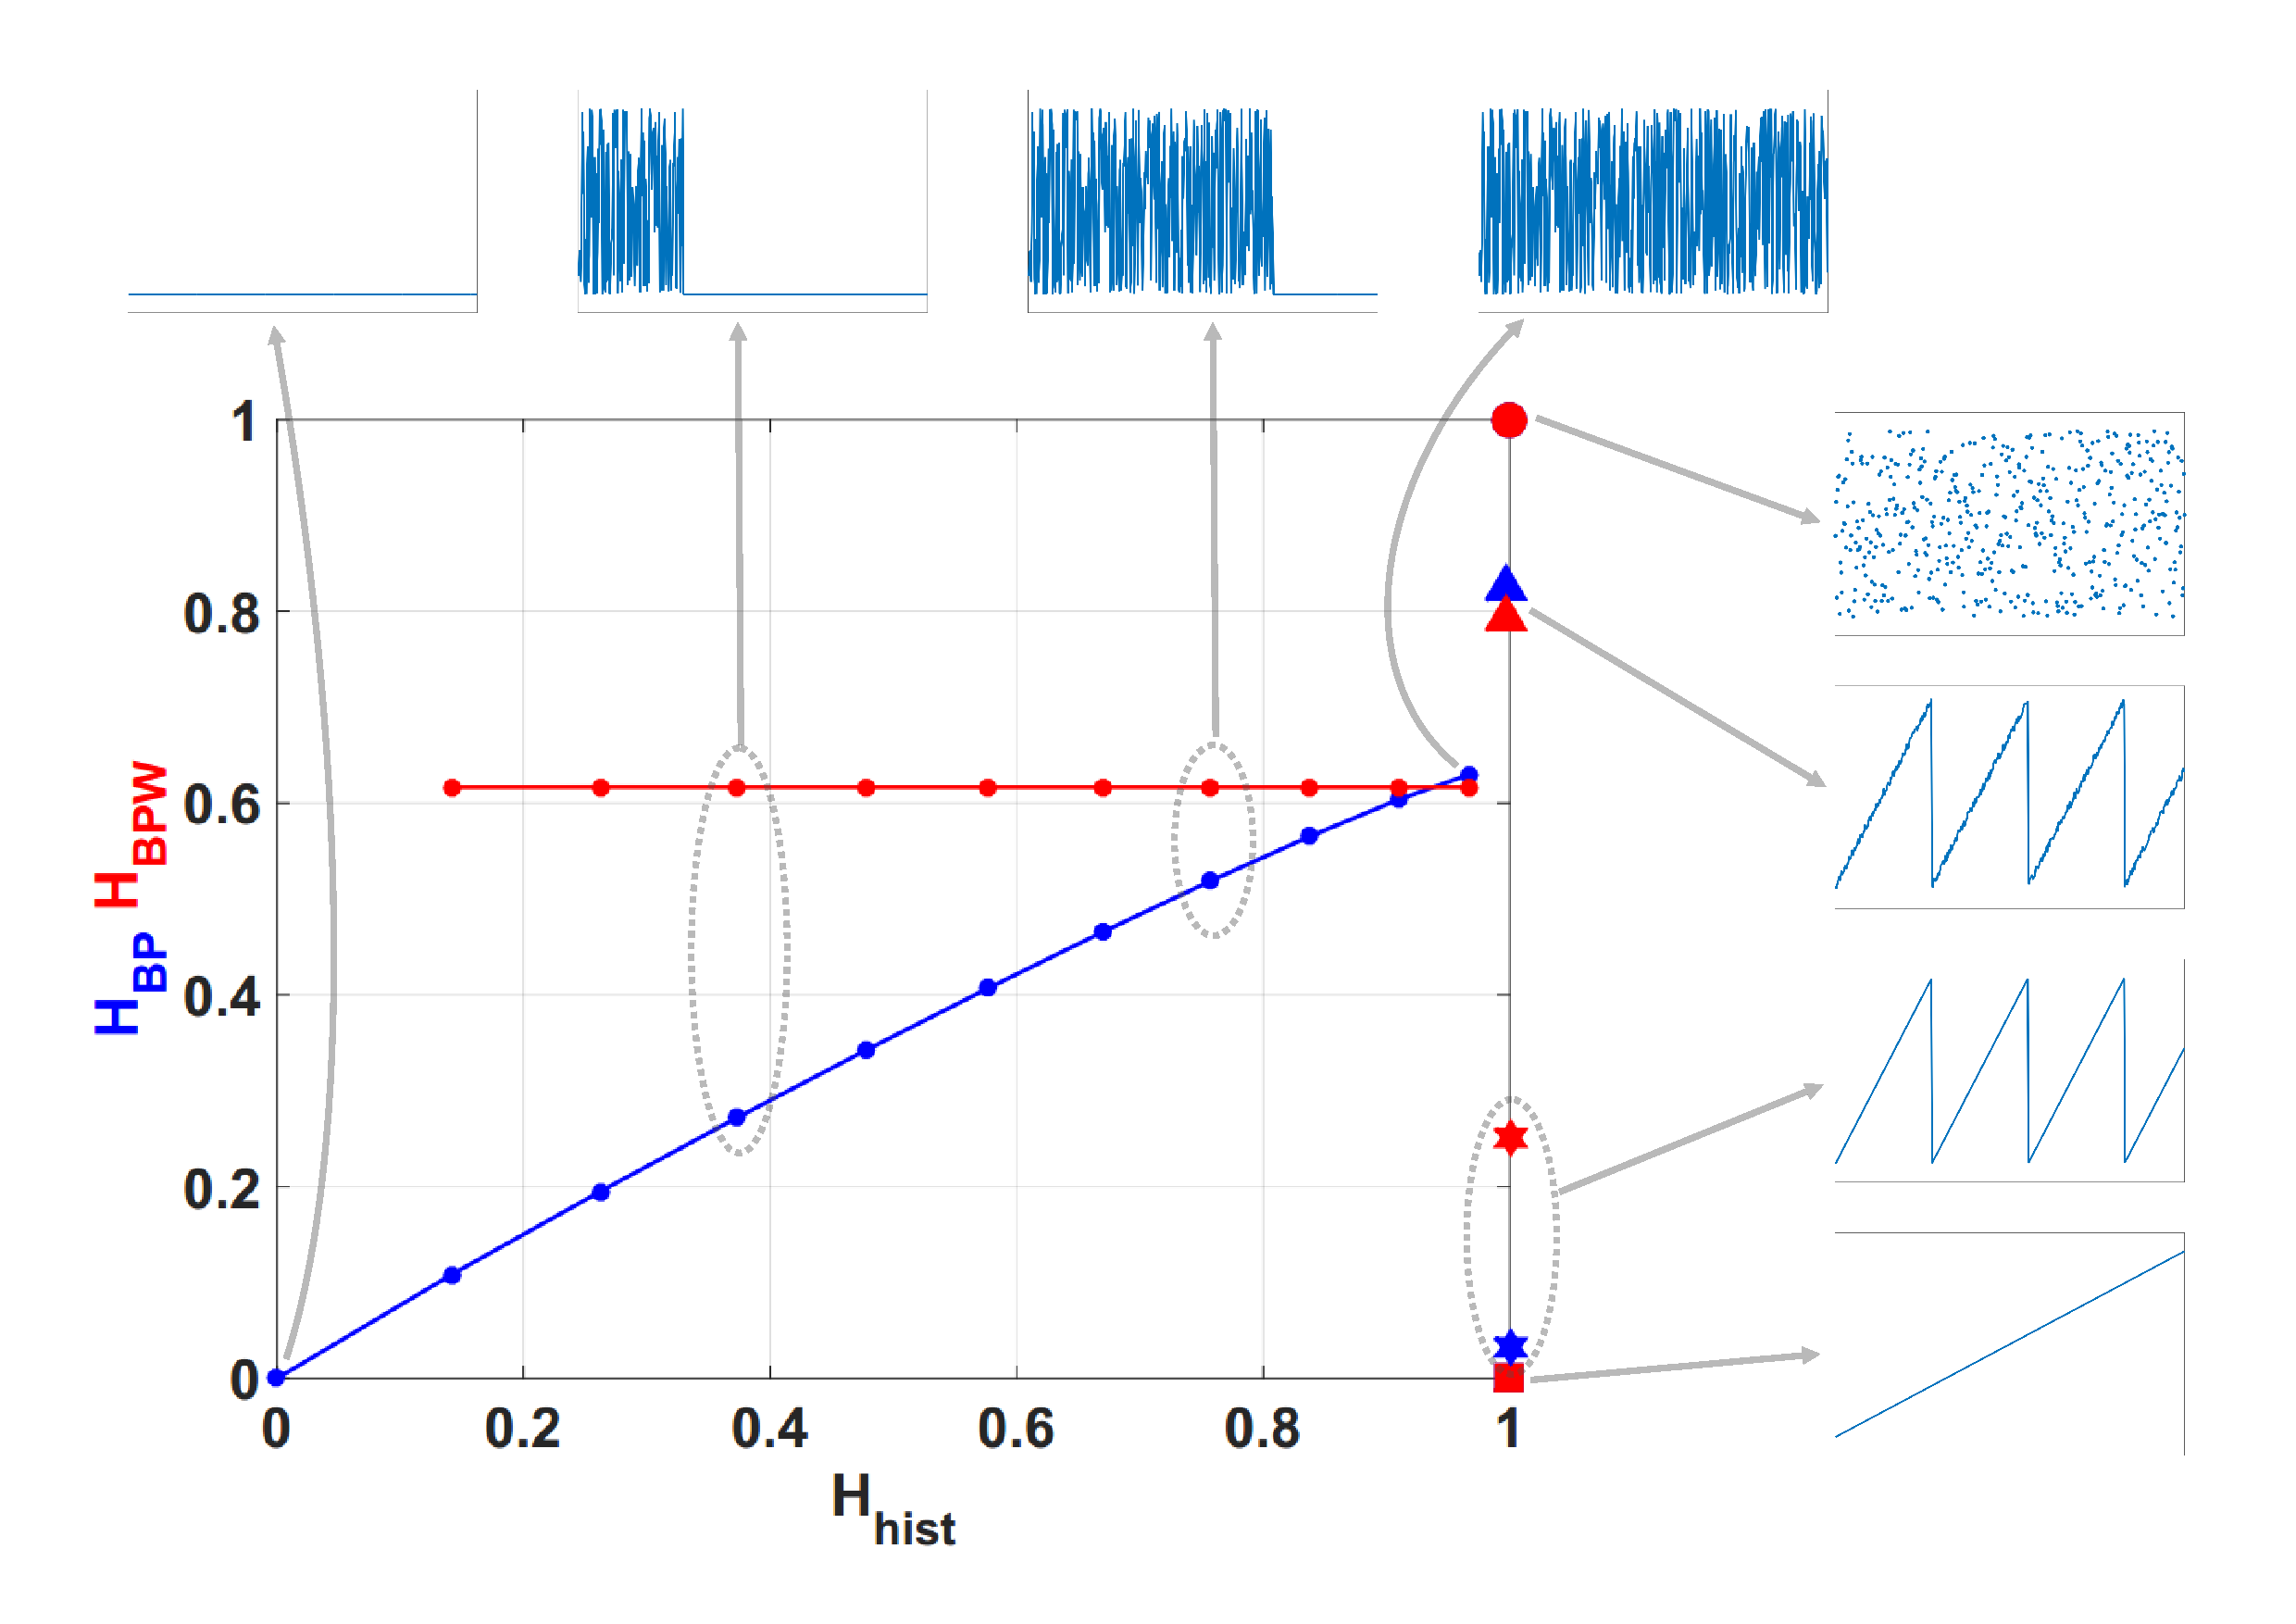
\includegraphics[width= .99\textwidth]{Fig1HHSignals}
	\caption{Causal-Non causal Entropy plane.}
\label{fig:HH}
\end{figure}
	
	
\begin{figure}[htpb]
	\centering		
	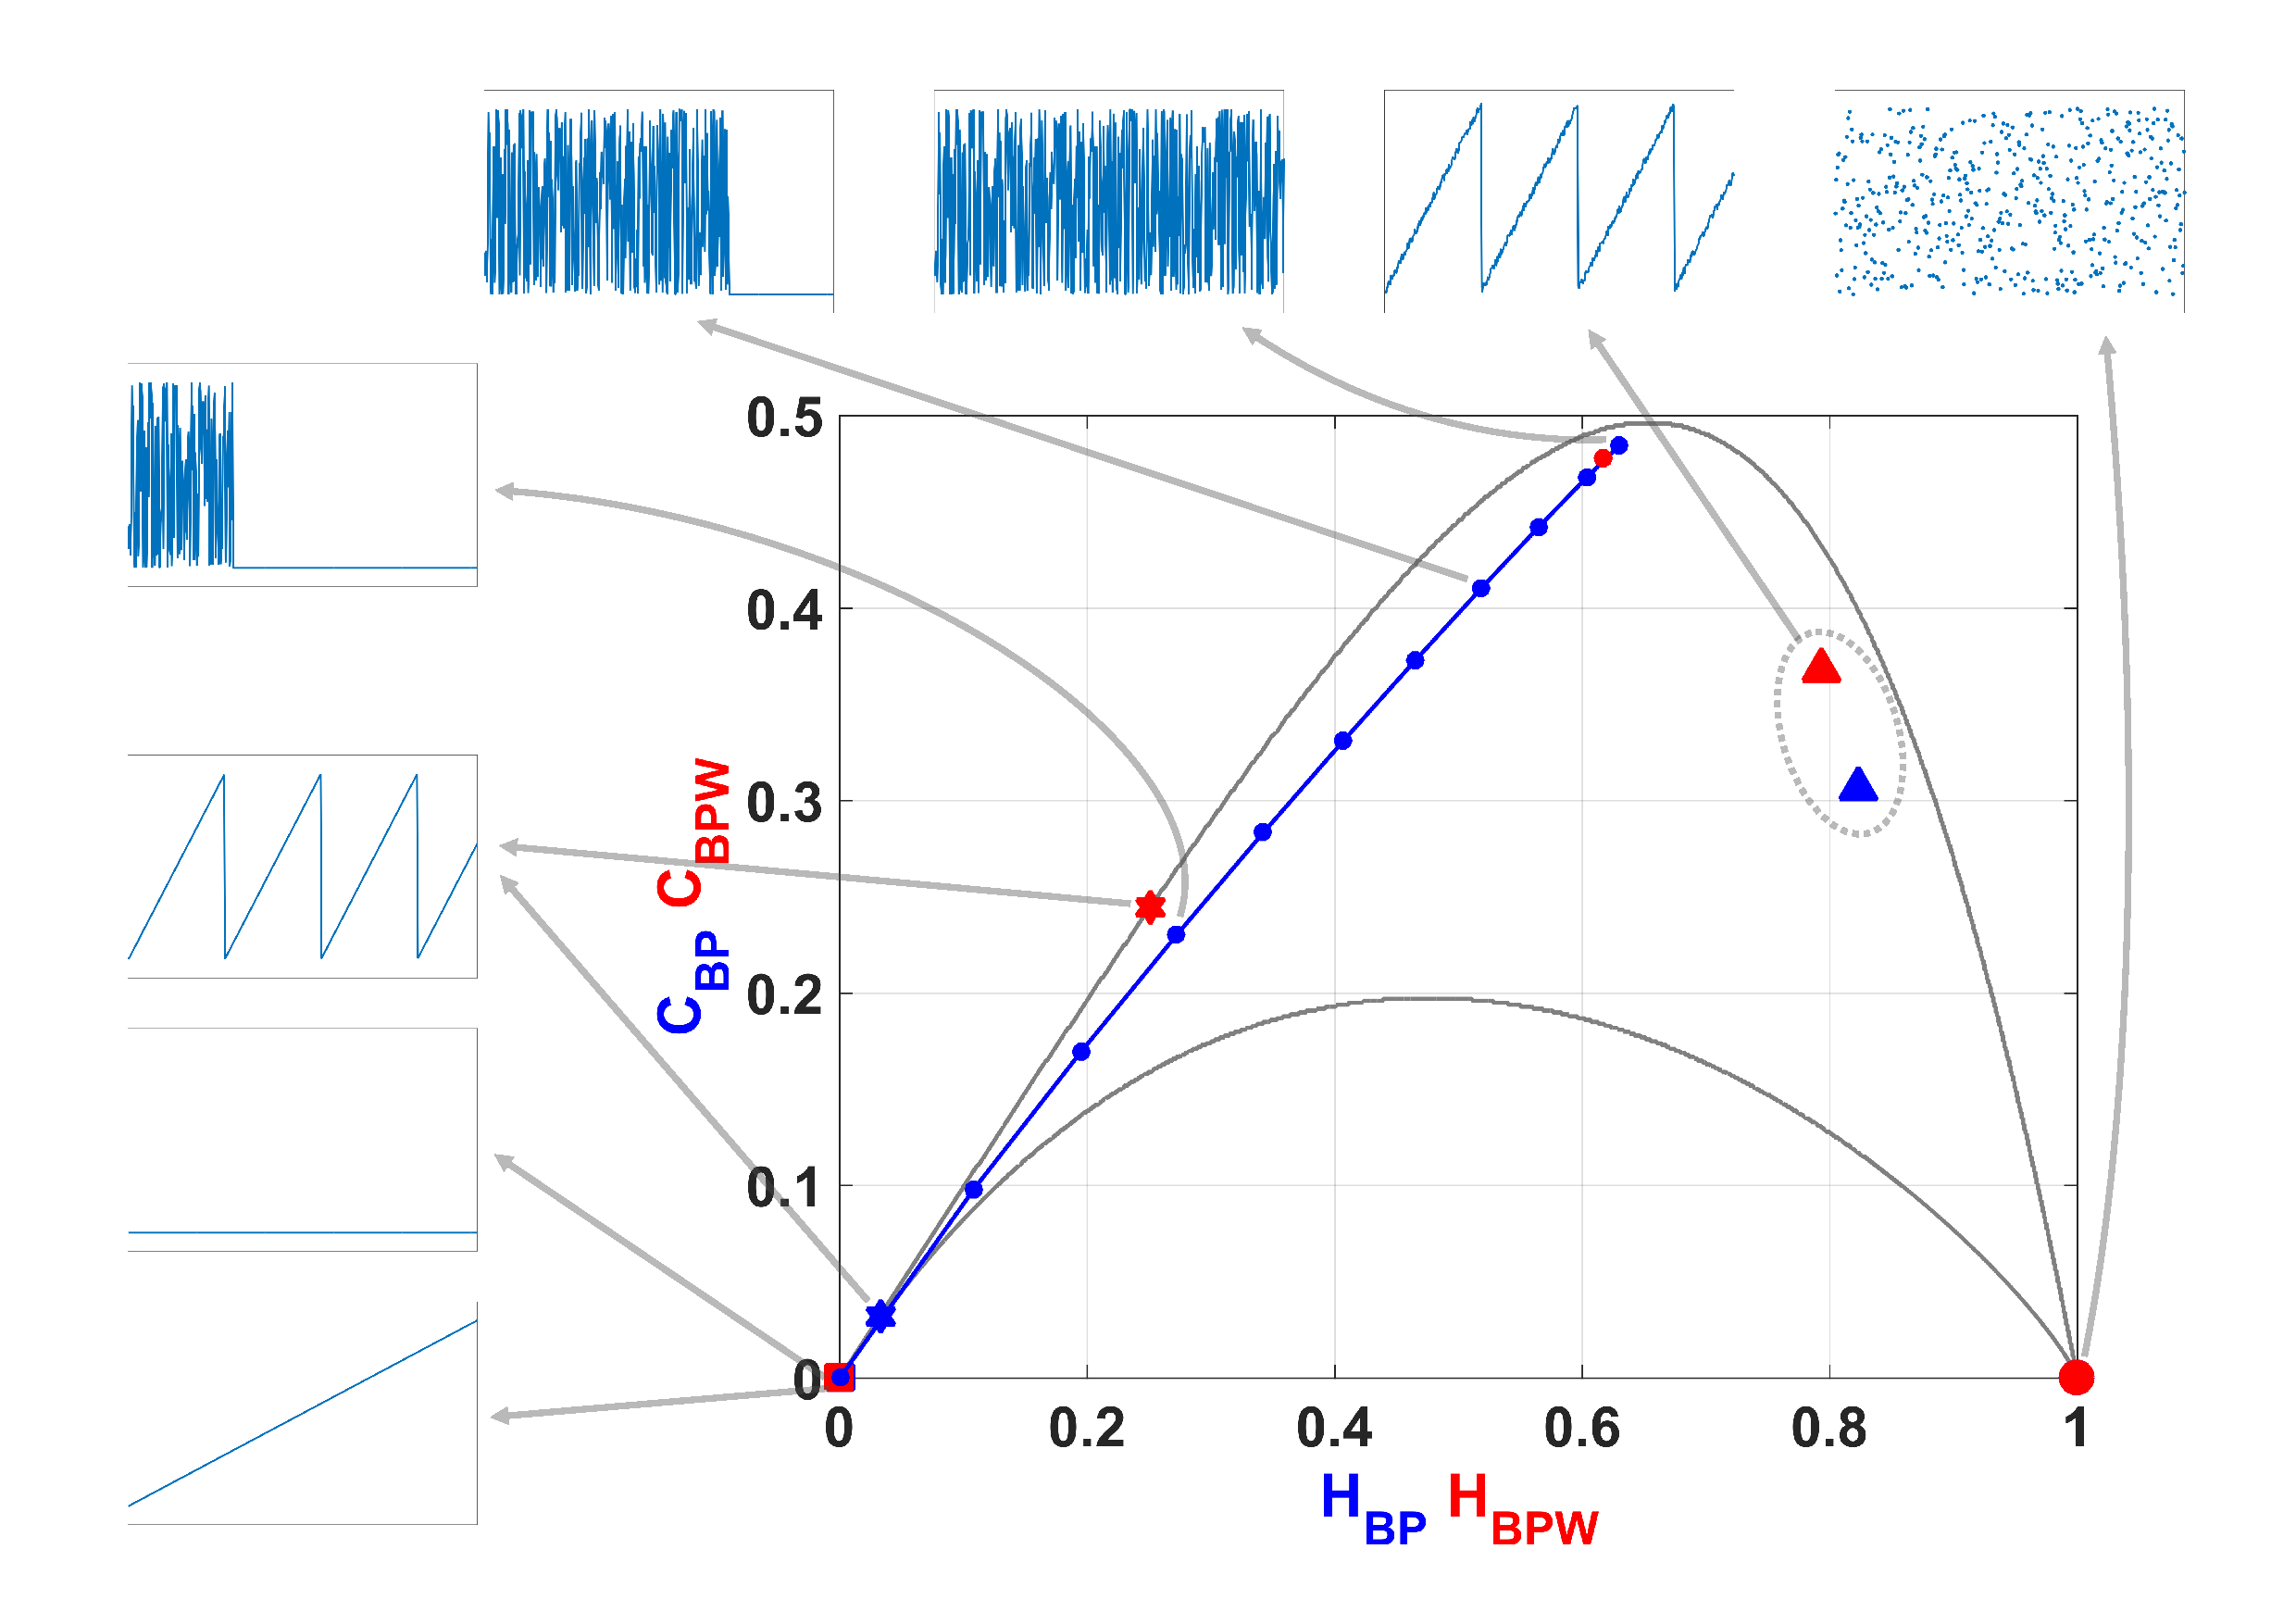
\includegraphics[width= .99\textwidth]{Fig1HCSignals}
	\caption{Causal Entropy-Complexity plane.}
	\label{fig:HC}
\end{figure}

We also used the number of missing patterns MP as a quantifier \cite{Rosso2012}.
As shown recently by Amig\'o {\it et al.} \cite{Amigo2006,Amigo2007,Amigo2008,Amigo2010}, in the case of deterministic maps, not all the possible ordinal patterns can be effectively materialized into orbits, which in a sense makes these patterns missing.
Indeed, the existence of these missing ordinal patterns becomes a persistent fact that can be regarded as a new dynamical property.
Thus, for a fixed pattern-length (embedding dimension $D$) the number of missing patterns of a time series (unobserved patterns) is independent of the series length $N$.
Remark that this independence does not characterize other properties of the series such as proximity and correlation, which die out with time \cite{Amigo2007,Amigo2010}.
A full discussion about the convenience of using these quantifiers is out of the scope of this work.
Nevertheless reliable bibliographic sources do exist \cite{DeMicco2008,Rosso2010,Rosso2012,Lopez-Ruiz1995,Martin2006,Wackerbauer1994,Rosso2007A}.




\section{Results}\label{sec:resultados}

Five pseudo chaotic maps were studied, two simple maps and three combination of them.
For each one using numbers represented by floating-point (80 bits of mantissa) and  fixed-point numbers with $1\leq B \leq 53$, where $B$ is the number of bits that represents the fractional part.
Time series were generated using $100$ randomly chosen initial conditions within their attraction domain (interval $[0,1]$), for each one of these $54$ number precisions.

The studied maps are logistic (LOG), tent (TENT), sequential switching between TENT and LOG (SWITCH) and skipping discarding the values in the odd positions (EVEN) or the values in the even positions (ODD) respectively.

Logistic map is interesting because is representative of the very large family of quadratic maps.
Its expression is:
%
\begin{equation}\label{eq:logimap}
x_{n+1}=4\,x_{n}(1-x_{n}) 
\end{equation}

\noindent with $x_n \in \mathbb{R}$.

Note that to effectively work in a given representation it is necessary to change the expression of the map in order to make all the operations in the chosen representation numbers. For example, in the case of LOG the expression in binary fixed-point numbers is:

\begin{equation}\label{eq:logimapB2}
x_{n+1}=4 \epsilon \,\text{floor}\left\{\frac{x_n(1-x_n)}{\epsilon}\right\}
\end{equation}

\noindent with $\epsilon = 2^B$ where $B$ is the number of bits that represents the fractional part.

The Tent map has been extensively studied in the literature because theoretically it has nice statistical properties that can be analytically obtained.
For example it is easy to proof that it has a uniform histogram and consequently an ideal $H_{hist}=1$.
The Perron-Frobenius operator and its corresponding eigenvalues and eigenfunctions may be also be analytically obtained for this map \cite{Lasota1994}.

This map is represented with the equation:
\begin{equation}\label{eq:tentmap}
x_{n+1}~=~ \left\{ \begin{array}{ll}
2~{x_n} &, \textrm{if ~$0\leq x_n\leq 1/2$}\\
2~(1-{x_n}) &, \textrm{if ~$1/2<x_n\leq 1$} 
\end{array} \right. 
\end{equation}
with $x_n \in \mathbb{R}$.

In base-2 fractional numbers rounding, equation (\ref{eq:tentmap}) becomes:
\begin{equation}\label{eq:tentdecbin}
x_{n+1}~=~ \left\{ \begin{array}{ll}
2~{x_n} &, \textrm{if $0\leq x_n\leq 1/2$}\\
\epsilon \; \text{floor}\{\frac{2~-~2~x_n}{\epsilon}\} &, \textrm{if $1/2<x_n\leq 1$} 
\end{array} \right. 
\end{equation}
with $\epsilon=2^{-B}$.

Switching, even skipping and odd skipping procedures are shown in Fig. \ref{fig:seq}.

\begin{figure}[htpb]
\centering	
	\includegraphics[height=0.4\textheight]{SwitchParImpar}
	\caption{Sequential switching between Tent and Logistic maps. In the figure are also shown even and odd skipping strategies.} \label{fig:seq}
\end{figure}

SWITCH map is expressed as:

\begin{equation}
\begin{cases}
x_{n+1}=
\begin{cases}
2\,x_n, &, \mbox{if } 0\leq x_n\leq 1/2 \\
2\,(1-x_n ) &, \mbox{if } 1/2<x_n\leq 1
\end{cases} \\
x_{n+2}=4\,x_{n+1}\,(1-x_{n+1})
\end{cases}\label{eq:SWITCH}
\end{equation}

\noindent with $x_n \in \mathbb{R}$ and $n$ an even number.

Skipping is a usual randomizing technique that increases the mixing quality of a single map and correspondingly increases the value of $H_{BP}$ and decreases $C_{BP} $ of the time series.
Skipping does not change the values of $H_{hist}$ because it are evaluated using the non causal PDF (normalized histogram of values) \cite{DeMicco2008}.

In the case under consideration we study even and odd skipping of the sequential switching of Tent and Logistic maps:
\begin{enumerate}
	\item Even skipping of the sequential switching of Tent and Logistic maps (EVEN).\\
	If $\{x_n; n=1,\dots,\infty\}$ is the time series generated by eq. \eqref{eq:SWITCH}, discard all the values in odd positions and retain the values in even positions.
	\item Odd skipping of the sequential switching of Tent and Logistic maps.
	If $\{x_n; n=1,\dots,\infty\}$ is the time series generated by eq. \eqref{eq:SWITCH}, discard all the values in even positions and retain all the values in odd positions.
\end{enumerate}

Even skipping may be expressed as the composition function TENT$\circ$LOG while odd skipping may be expressed as LOG$\circ$TENT.
The evolution of period as function of precision was reported in \cite{Nagaraj2008}.

Let us detail our results for each of these maps.

\subsection{Period as a function of binary precision}

Grebogi and coworkers \cite{Grebogi1988} have studied how the period $T$ is related with the precision.
There they saw that the period $T$ scales with roundoff $\epsilon$ as $T\sim\epsilon^{-d/2}$ where $d$ is the correlation dimension of the chaotic attractor.

Nagaraj \textit{et als}. \cite{Nagaraj2008} studied the case of switching between two maps.
They saw that the period $T$ of the compound map obtained by switching between two chaotic maps is higher than the period of each map and they found that a random switching improves the results.
Here we have considered sequential switching to avoid the use of another random variable, because it can include its own statistical properties in the time series.

Fig. \ref{fig:period} shows  $T$ vs. $B$ in semi logarithmic scale.
We run the attractor from $100$ randomly chosen initial conditions
The figure show: $100$ red points for each fixed-point precision ($1\geq B \geq 53$) and in black their average (dashed black line connecting black dots).
The experimental averaged points can be fitted by a straight line (in blue) expressed as $\log_10 T=m B + b$ where $m$ is the slope and $b$ is the $y$-intercept.
Results for the rest of considered maps are summarized in Table \ref{tabla:periodos}.

\begin{figure}[H]
\centering	
	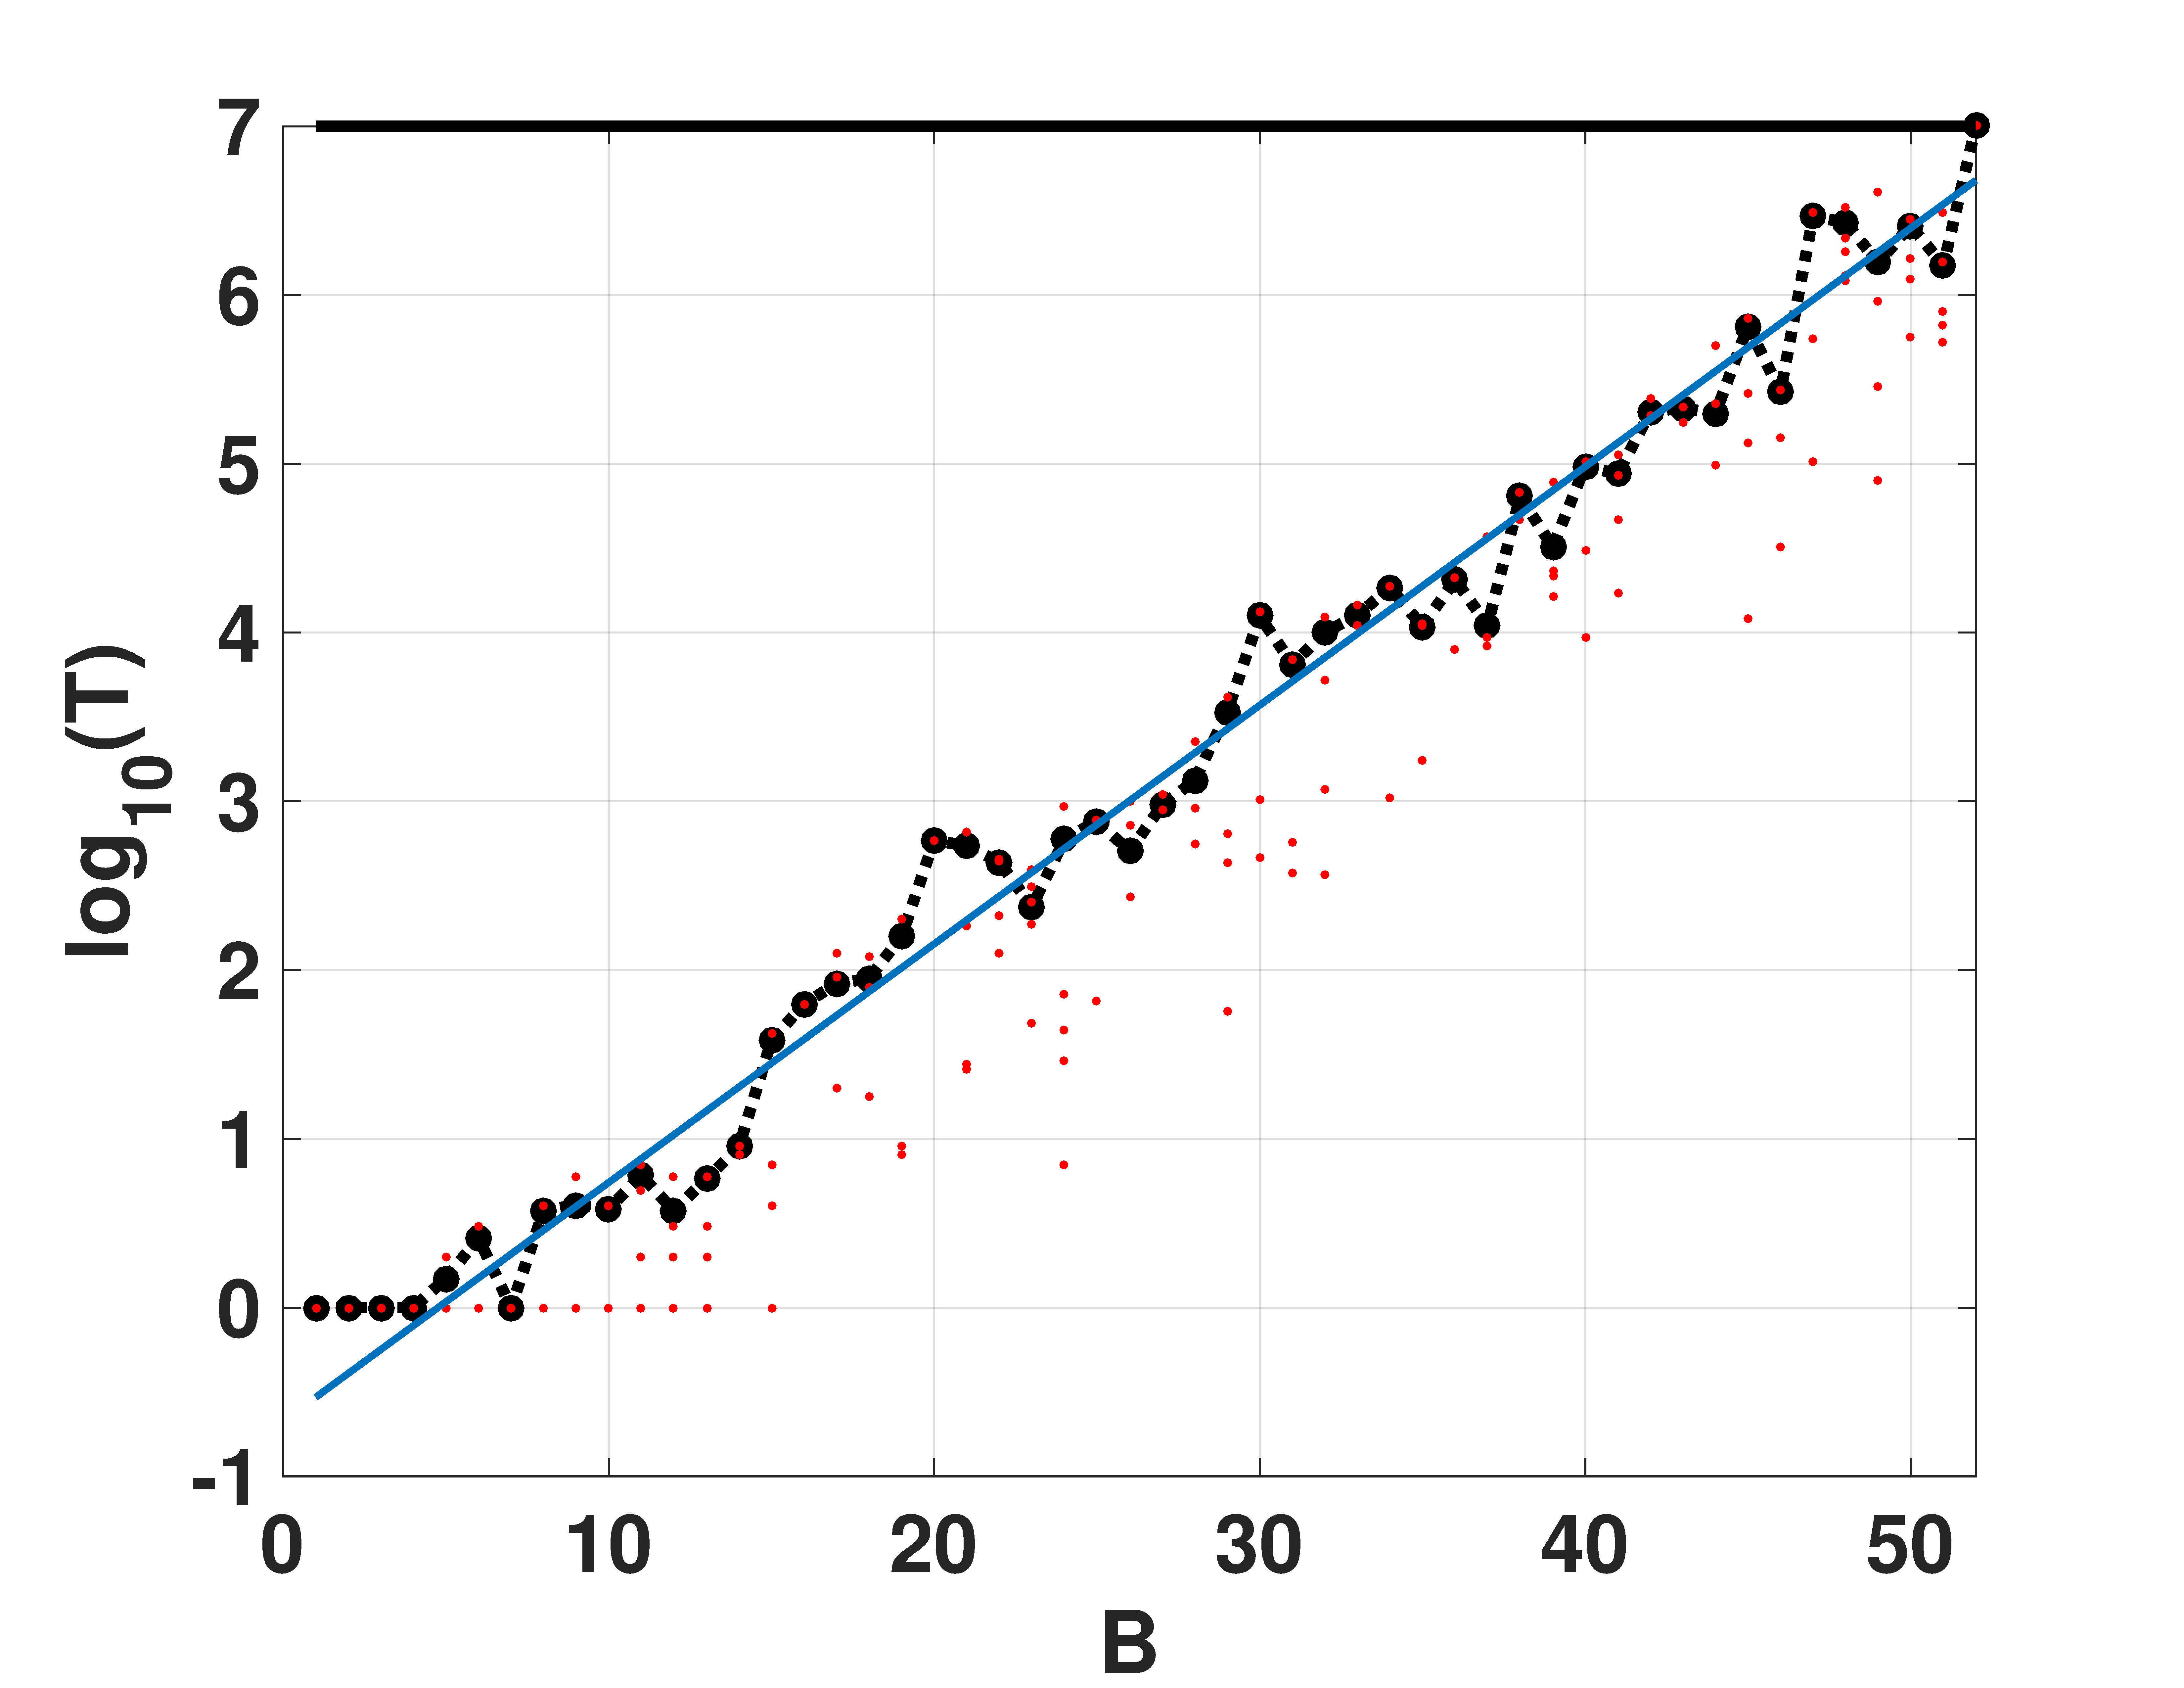
\includegraphics[width=.49\textwidth]{Period_Log}
	\caption{Period as function of precision in binary digits (see text).}
	\label{fig:period}
\end{figure}

\begin{table}[H]
\centering	
	\caption{Period $T$ as a function of $B$ for the maps considered}
	\vspace{1em}
	\begin{tabular}{lll}
		\hline\noalign{\smallskip}
		map 	& m 	& b  \\
		\noalign{\smallskip}\hline\noalign{\smallskip}
		TENT	&0 		& 0 \\
		LOG 	&0.139 	& -0.6188 \\
		SWITCH 	&0.1462 & -0.5115 \\
		EVEN 	&0.1447 & -0.7783 \\
		ODD 	&0.1444 & -0.7683 \\
		\noalign{\smallskip}\hline
	\end{tabular}
	\label{tabla:periodos}	
\end{table}

Results are compatible for those obtained in \cite{Nagaraj2008}.
Switching between maps increases the period $T$ but skipping procedure decreases by almost half.

\subsection {Quantifiers of simple maps}\label{subsec:SimpleMaps}
Here we report our results for both simple maps, LOG and TENT

\subsubsection{Logistic map (LOG)} \label{subsubsec:log}

Logistic map is interesting because is representative of the very large family of quadratic maps.
Its expression is:
\begin{equation}\label{eq:logimap}
 x_{[n+1]}=4x_{[n]}(1-x_{[n]}) \,
\end{equation}
with $x_n\in\mathcal{R}$.

Note that to effectively work in a given representation it is necessary to change the expression of the map in order to make all the operations in the chosen representation numbers. For example, in the case of LOG the expression in binary fixed point numbers is:
\begin{equation}\label{eq:logimapB2}
x_{n+1}=4 \epsilon floor\{\frac{x_n(1-x_n)}{\epsilon}\} \,
\end{equation}
with $\epsilon = 2^B$ where $B$ is the number of bits that represents the fractional part.

According as B grows, statistical properties vary until they stabilize.
Figs. \ref{fig:LOG_QuantiB} (a) to (f) show the statistical properties of LOG map in floating point and fixed point representation.
All these figures show: $100$ red points for each fixed point precision ($B$) and in black their average (dashed black line connecting black dots), $100$ horizontal dashed blue lines that are the results of each run in floating point and a black solid line their average.
In this case, all the lines of the floating point are overlapped.

For $B\geq 30$ the value of $H_{val}$ remains almost identical to the values for the floating point representation whereas $H_{BP}$ and $C_{BP}$ stabilizes at $B>21$.
Their values are: $<H_{val}>=0.9669$; $<H_{BP}>=0.6269$; $<C_{BP}>=0.4843$.
Note that the stable value of missing patterns $MP=645$ makes the optimum $H_{BP} \leq ln(75)/ln(720) \simeq 0.65$.
Then, $B=30$ is the most convenient choice because an increase in the number of fractional digits does not improve the statistical properties.

Some conclusions can be drawn regarding \textit{BP} and \textit{BPW} quantifiers.
For $B=1, 2, 3$ and $4$, the averaged $BP$ quantifiers are almost $0$ while the averaged $BPW$ quantifiers can not be calculated (seein Figs. \ref{fig:LOG_QuantiB} c and e the missing black dashed line).
For those sequences where the initial condition where $0$ all iterations result to be a sequence of $0$s (the fixed point of the map), this happens very likely with small precisions because of the roundoffs.

When $B$ increases, $B=7, 9$ and $12$, the used initial conditions are rounded to zero less frequently.
So the generated sequences start from some value but many of them fall to zero with a short transitory.
This can be seen in Figs. c and e, $BPW$ shows high dispersion unlike $BP$ quantifiers.
This is because $BPW$ procedure takes into account only the transient discarding fixed points, unlike $BP$ procedure that considers all the sequence. 
 
\textcolor{red}{ESTE PÁRRAFO VA A DESAPARECER CON LONG DOUBLE, O NO?, ADEMÁS DISTRAE DEL FOCO DEL TRABAJO. HAY QUE BUSCARLE UN LUGAR EN EL PAPER}
Finally, for $B = 45, 49, 51$ and $52$ some $BP$ quantifiers have a low value, but $BPW$ quantifiers have a more predictible behavior, we can see that these atractors fall to a fixed point with a long transitory.
In this behaviour is due to the employed plataform.
The operation miltiplication needs the double of bits to be represented but the machine has only $64$.
Acá lo que quiero decir es que en las figuras \ref{fig:LOG_QuantiB} a, b y d las corridas con punto fijo tienen alta dispersión y aparecen algunas con valores muy bajos.
Esto es por que la aritmética de punto fijo la estamos queriendo generar artificialmente con una variable de tipo double que tiene una mantisa de 53 bits.
Entonces en la multiplicación (que duplica la cantidad de bits necesarios) se pierden muchos fraccionarios.
Lo mismo pasa si se usa el tipo float, que tiene 27 bits de mantisa pero mucho antes, a partir de B>24+-.
Con long double debería desaparecer.
Entonces hay que tener en cuenta esto cuando se simula punto fijo con la computadora, en los mapas que halla multiplicaciones.

\begin{figure}
	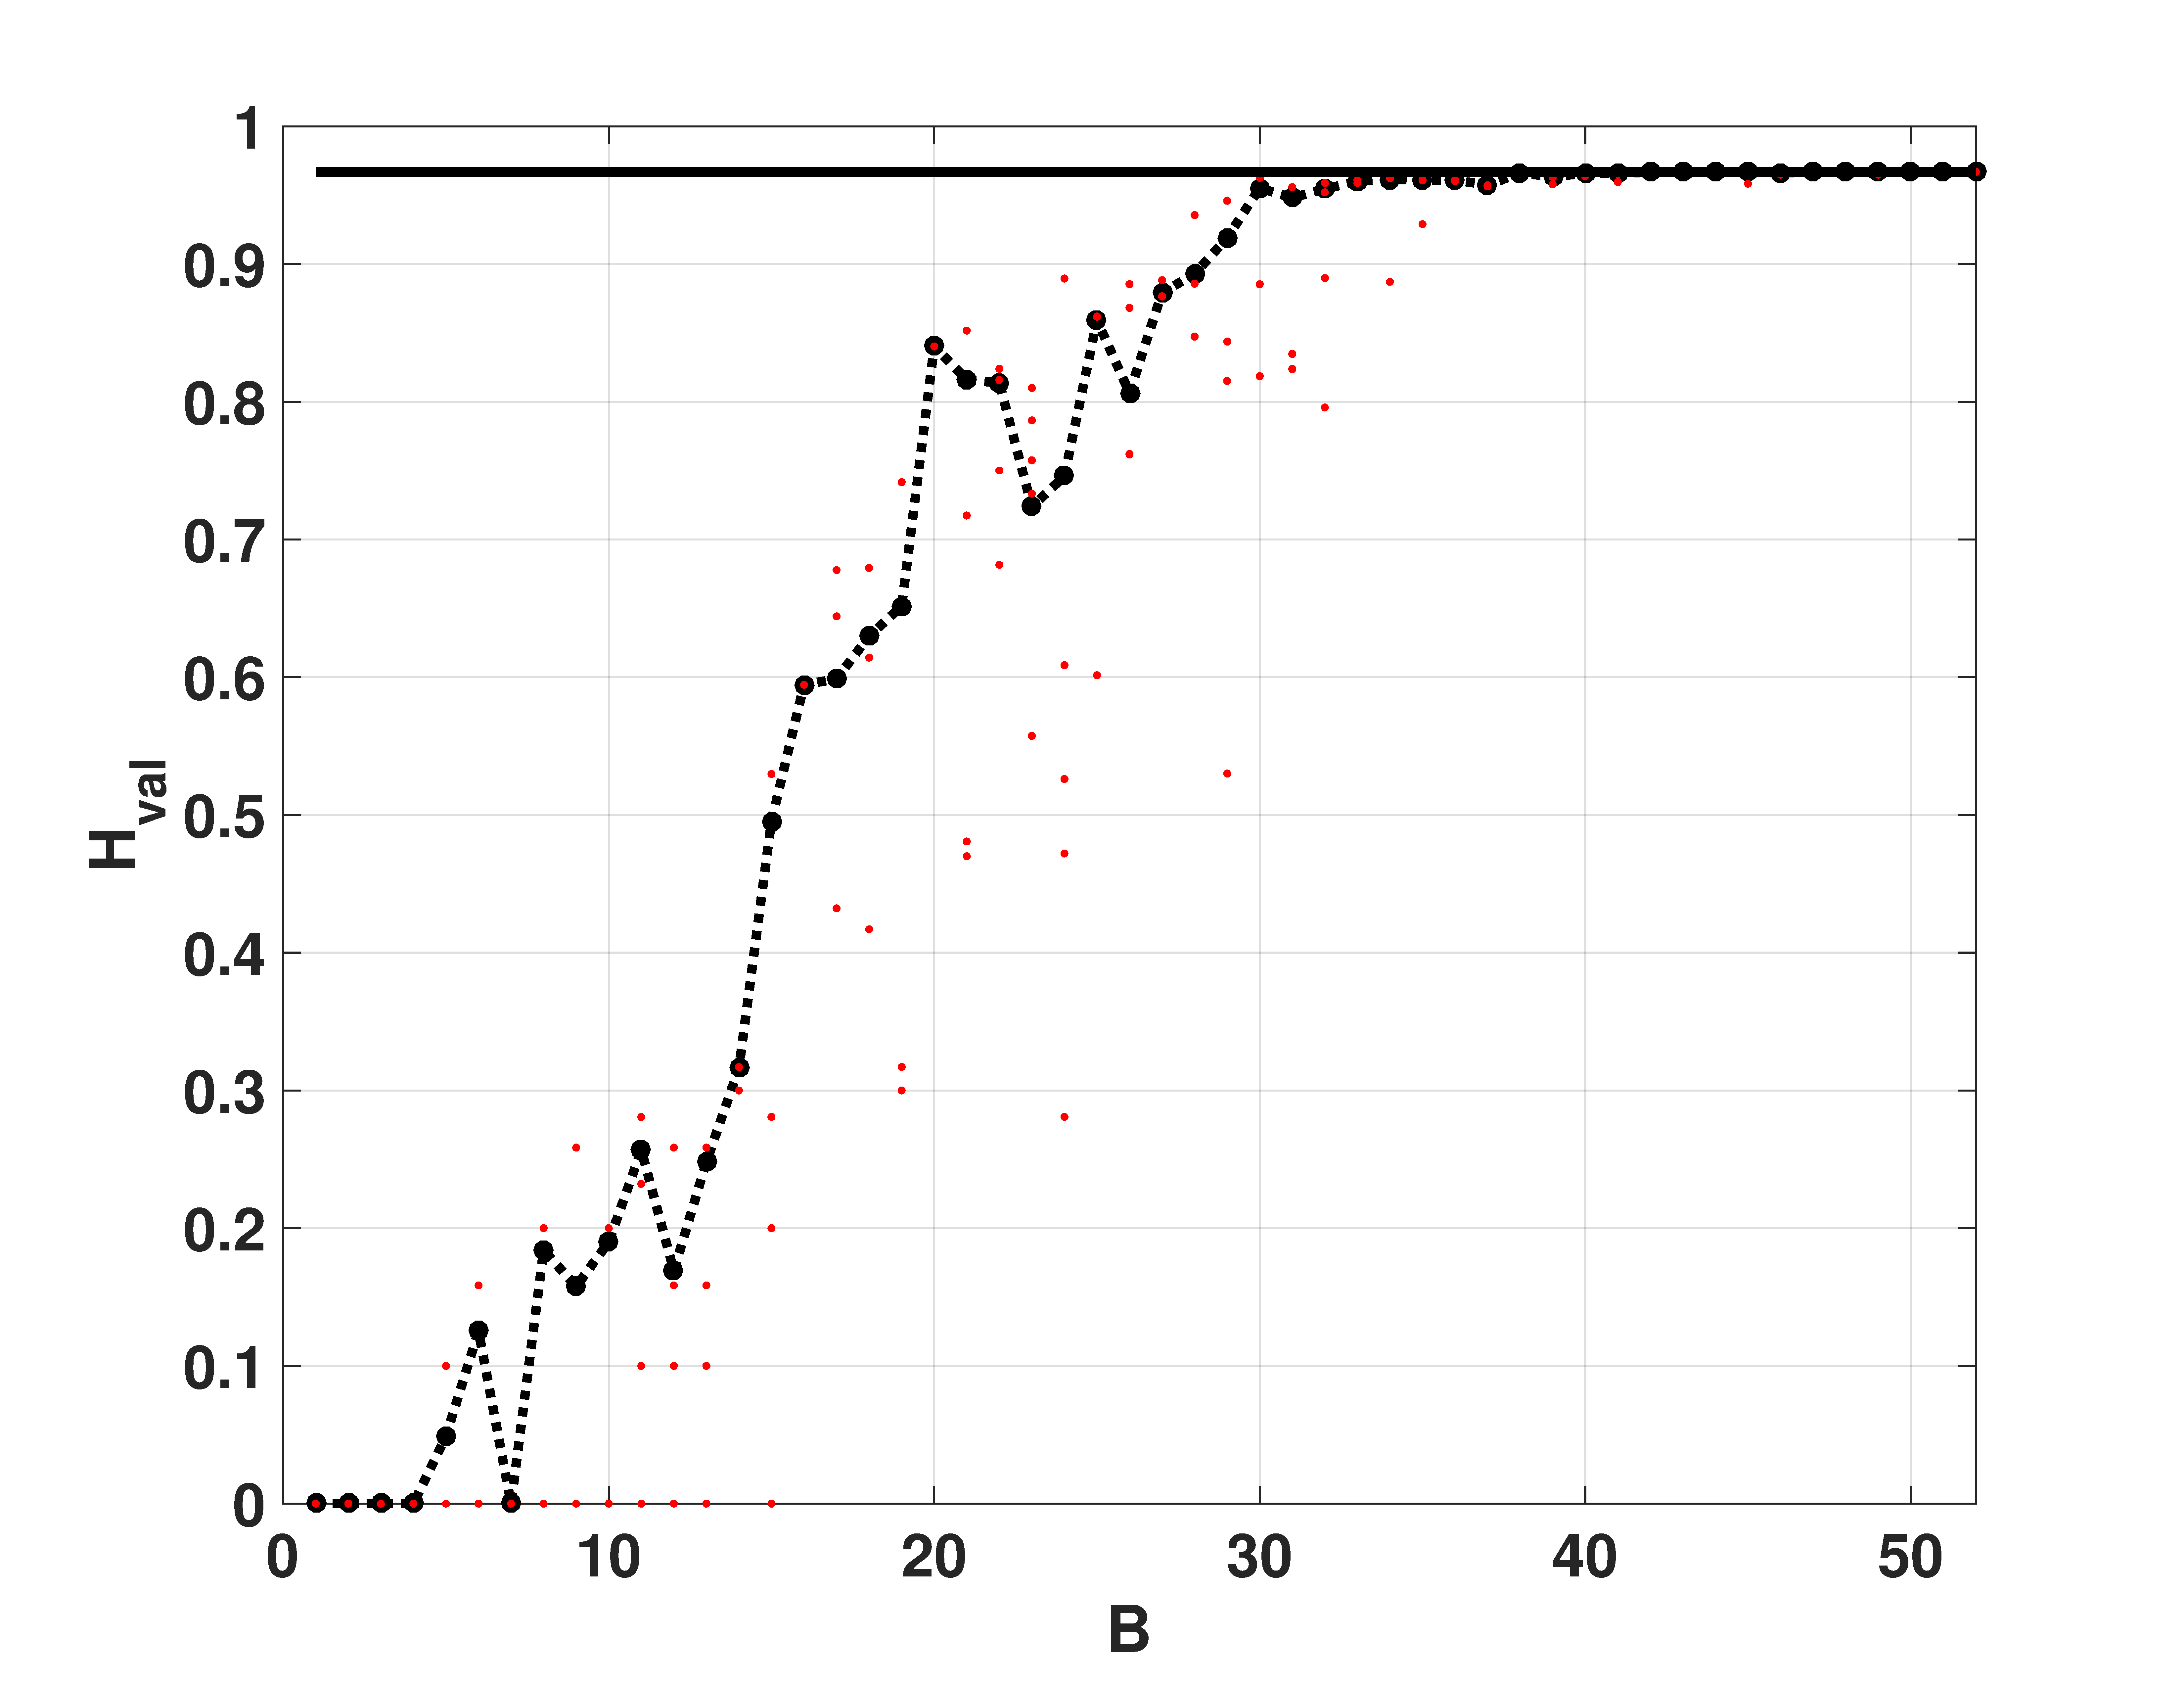
\includegraphics[width= .49\textwidth]{Hval_Log}
	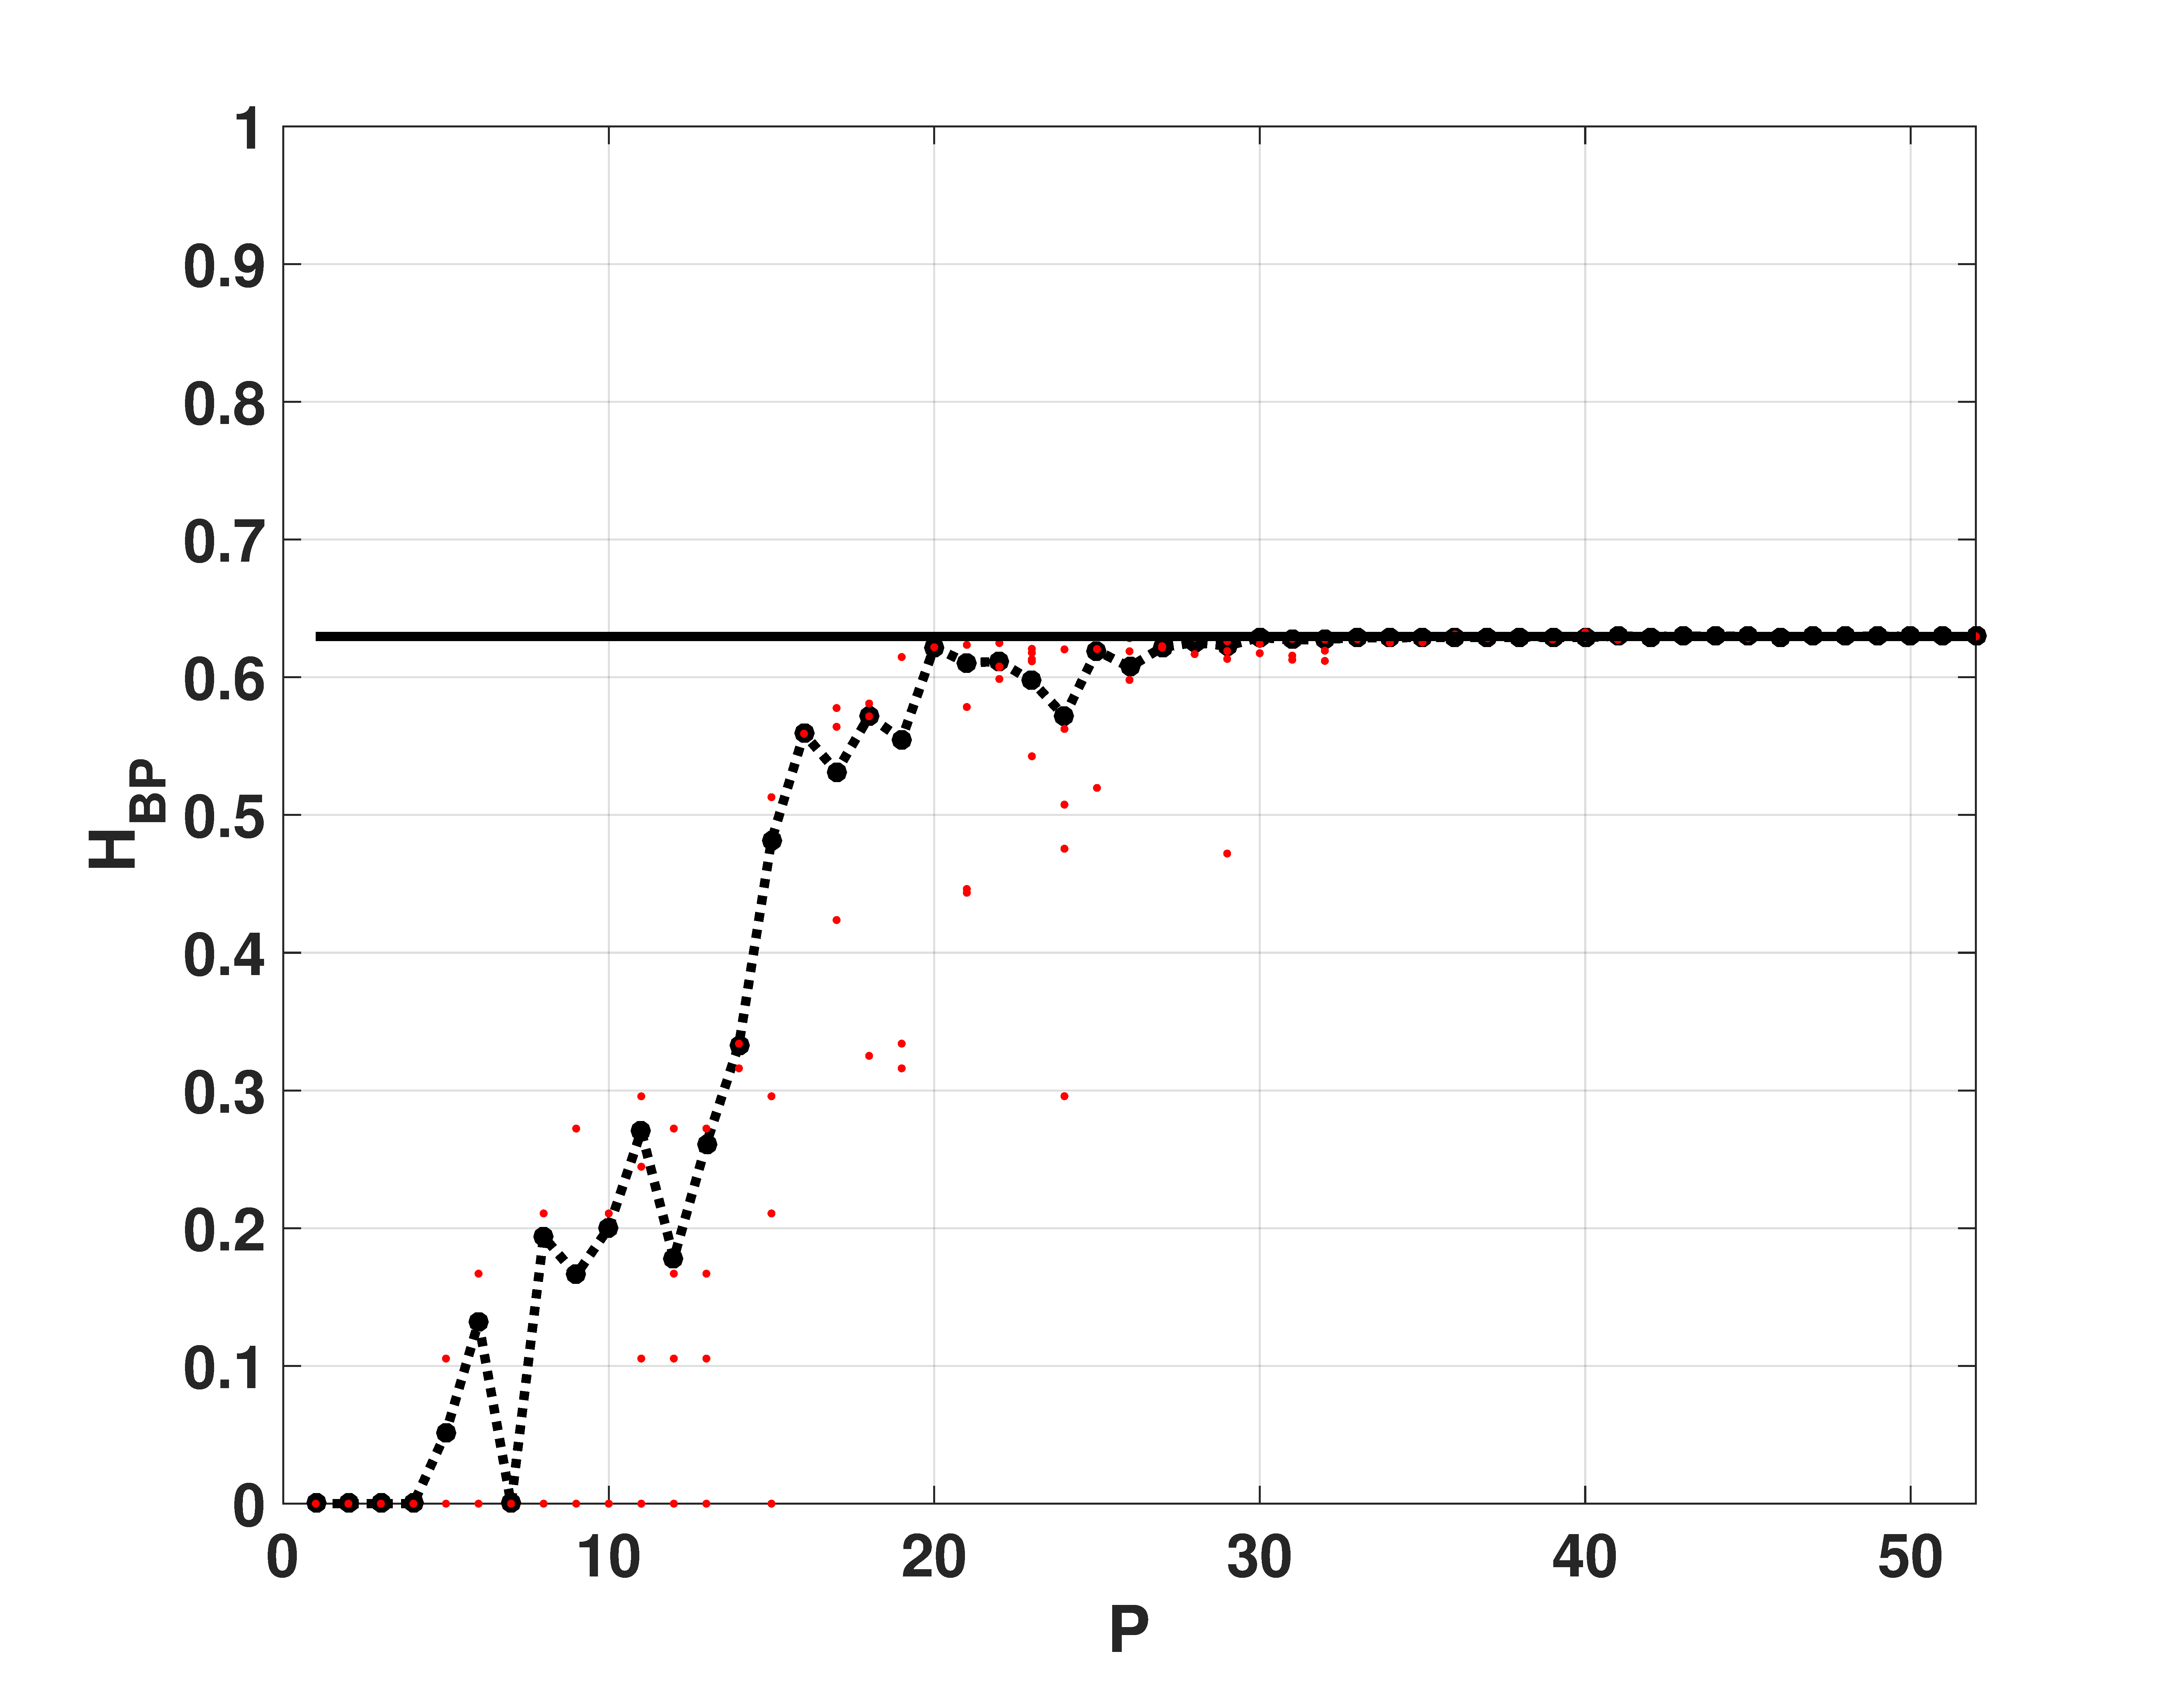
\includegraphics[width= .49\textwidth]{Hbp_Log}
	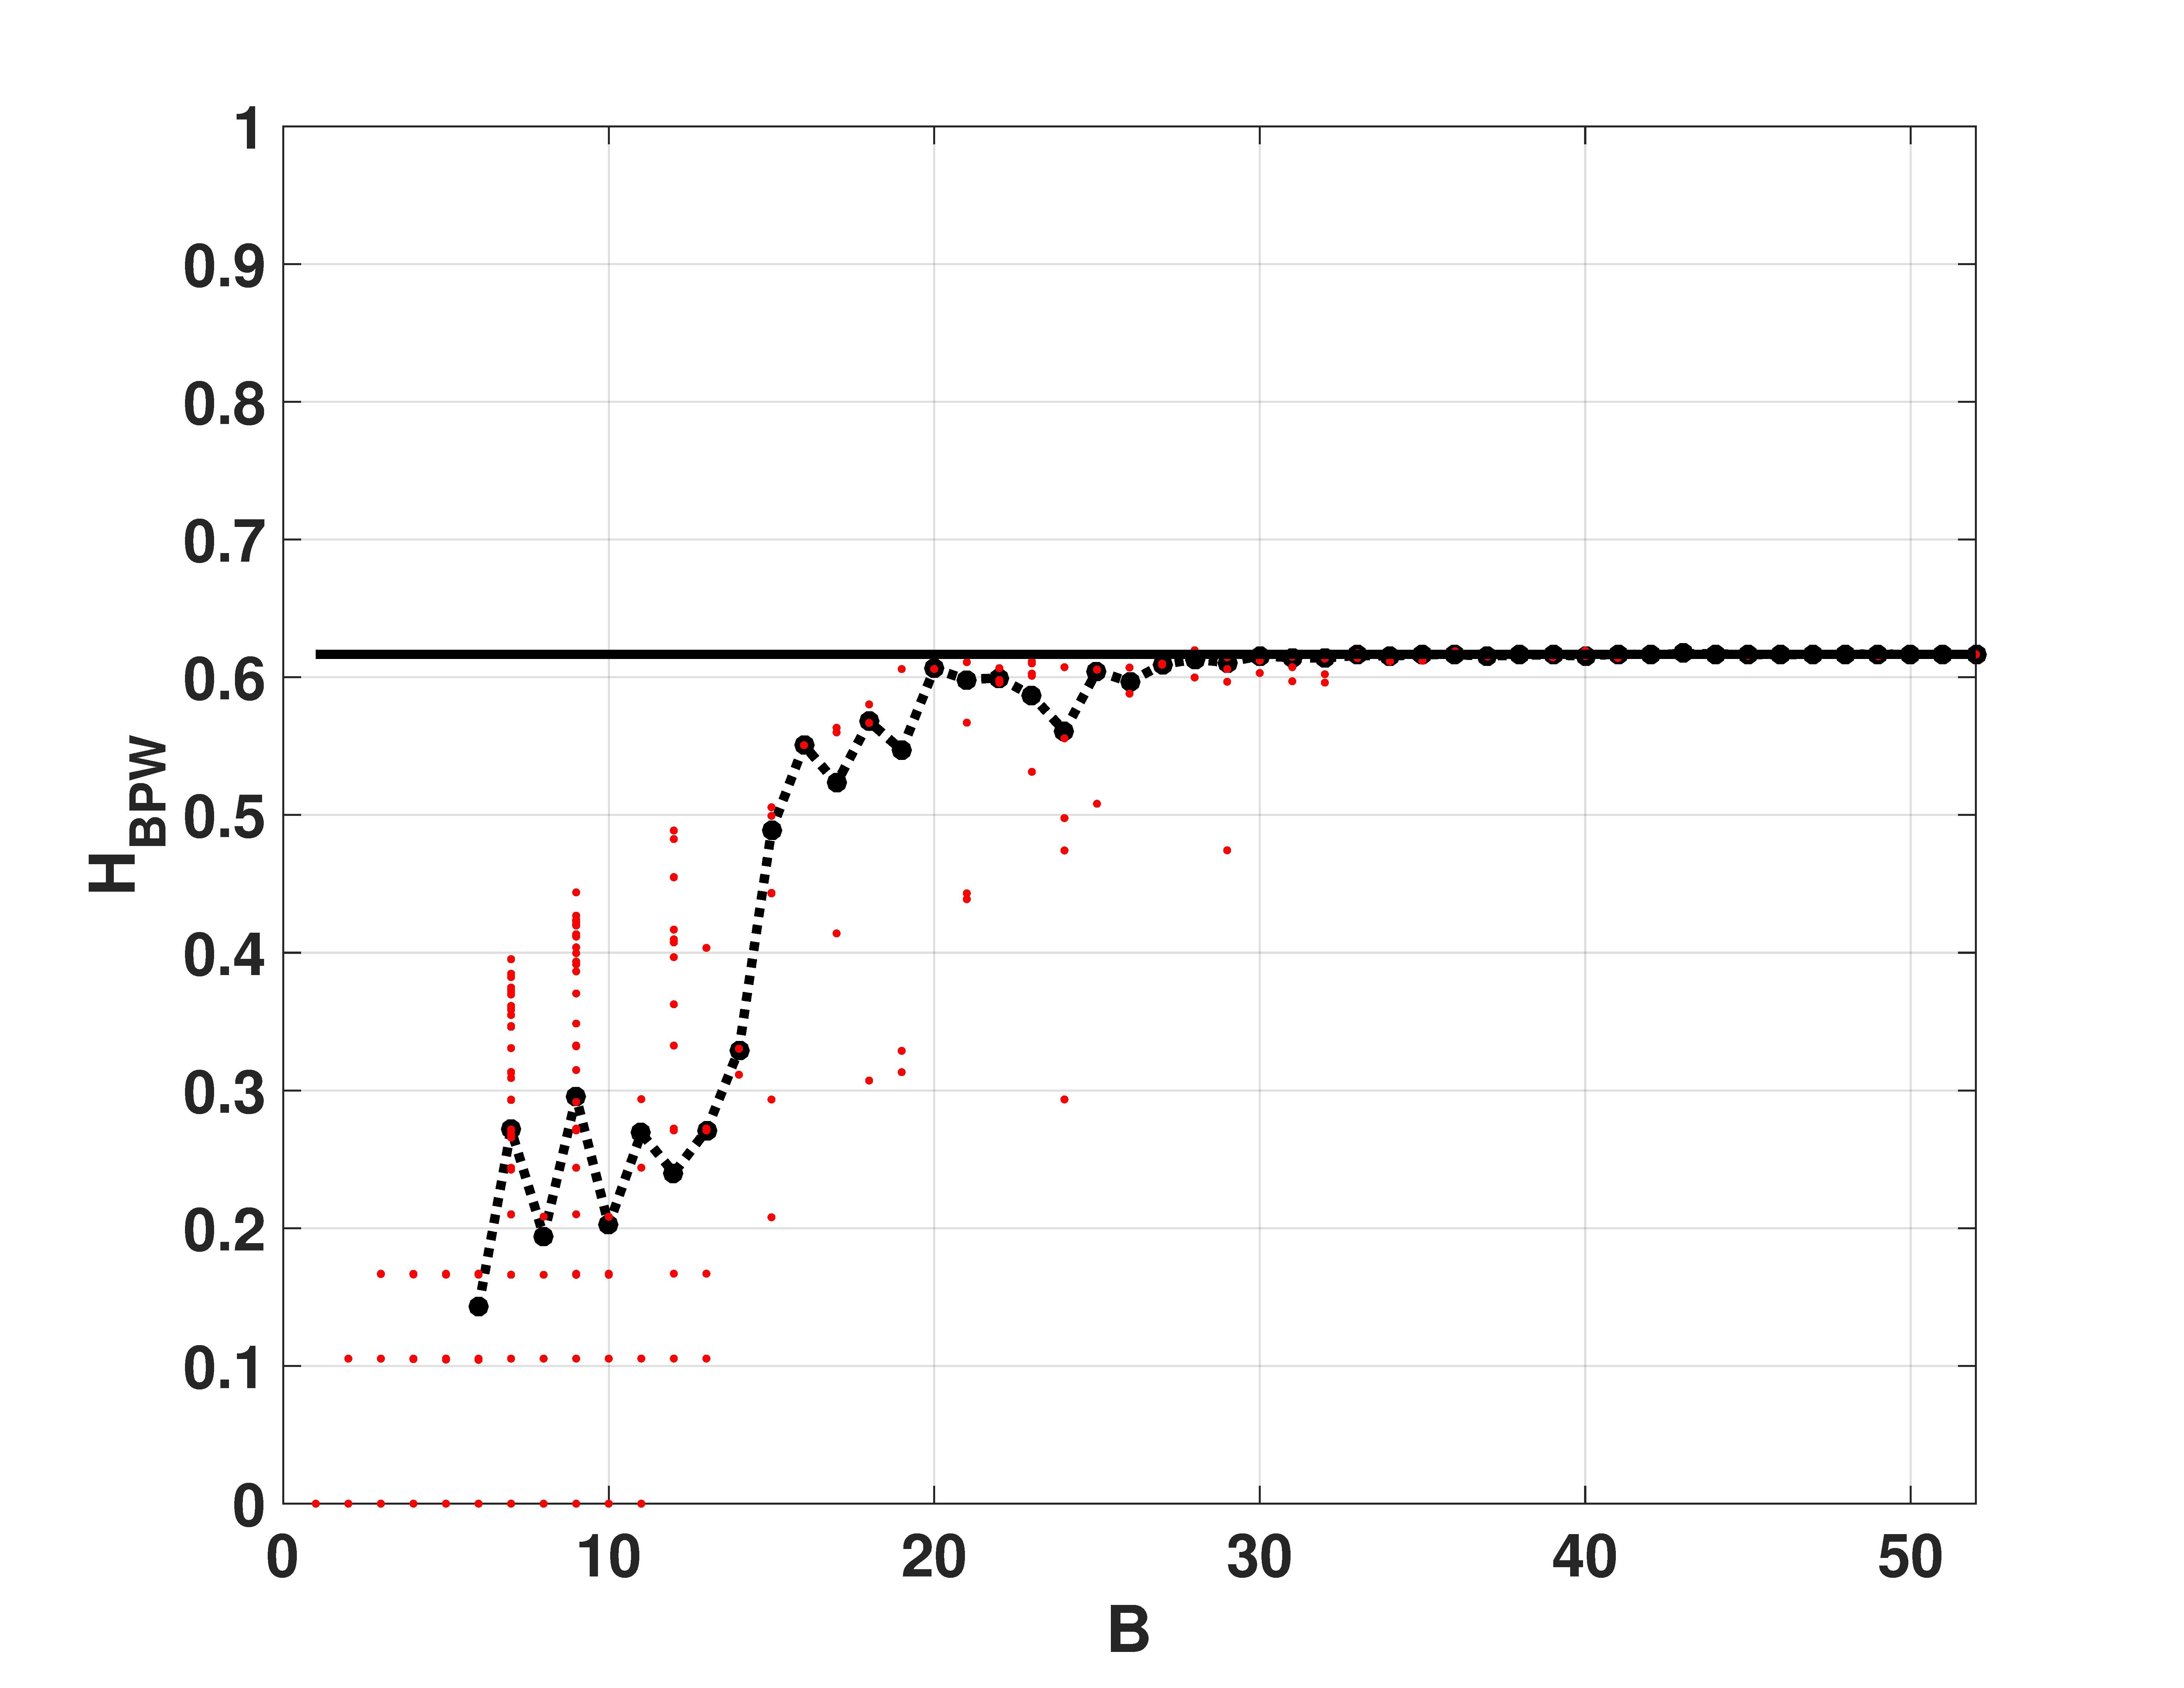
\includegraphics[width= .49\textwidth]{Hbpw_Log}
	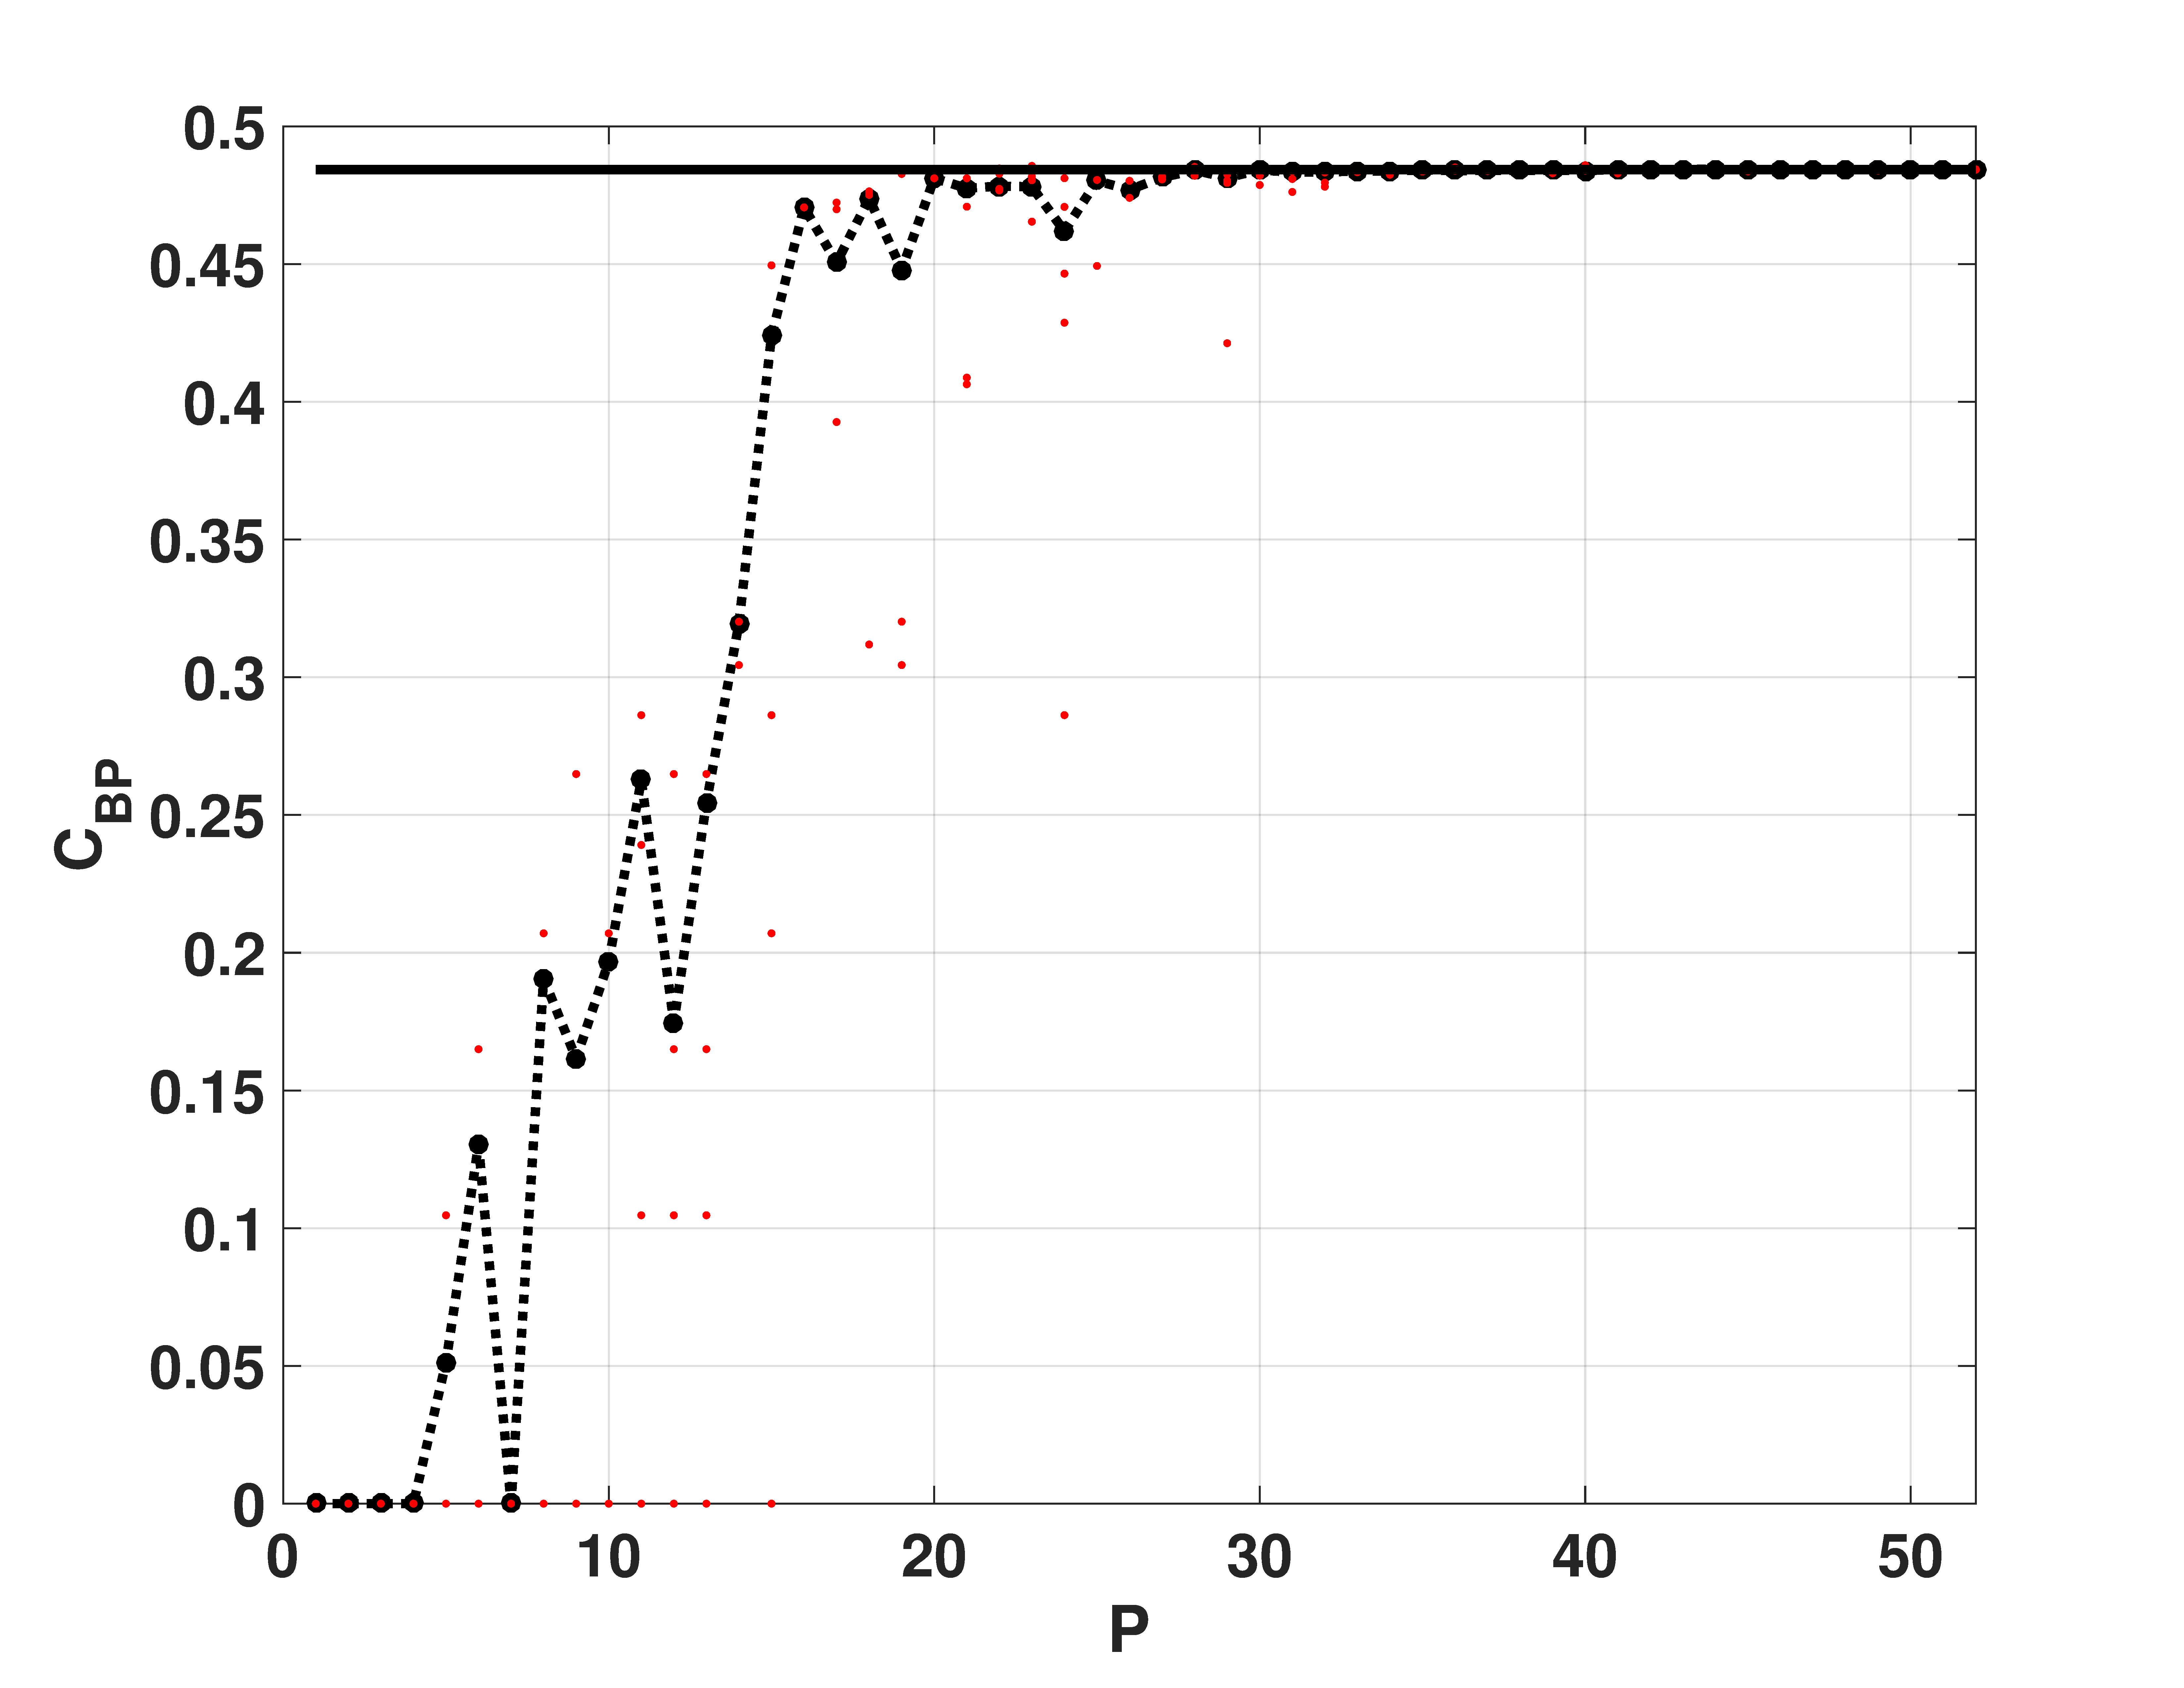
\includegraphics[width= .49\textwidth]{Cbp_Log}
	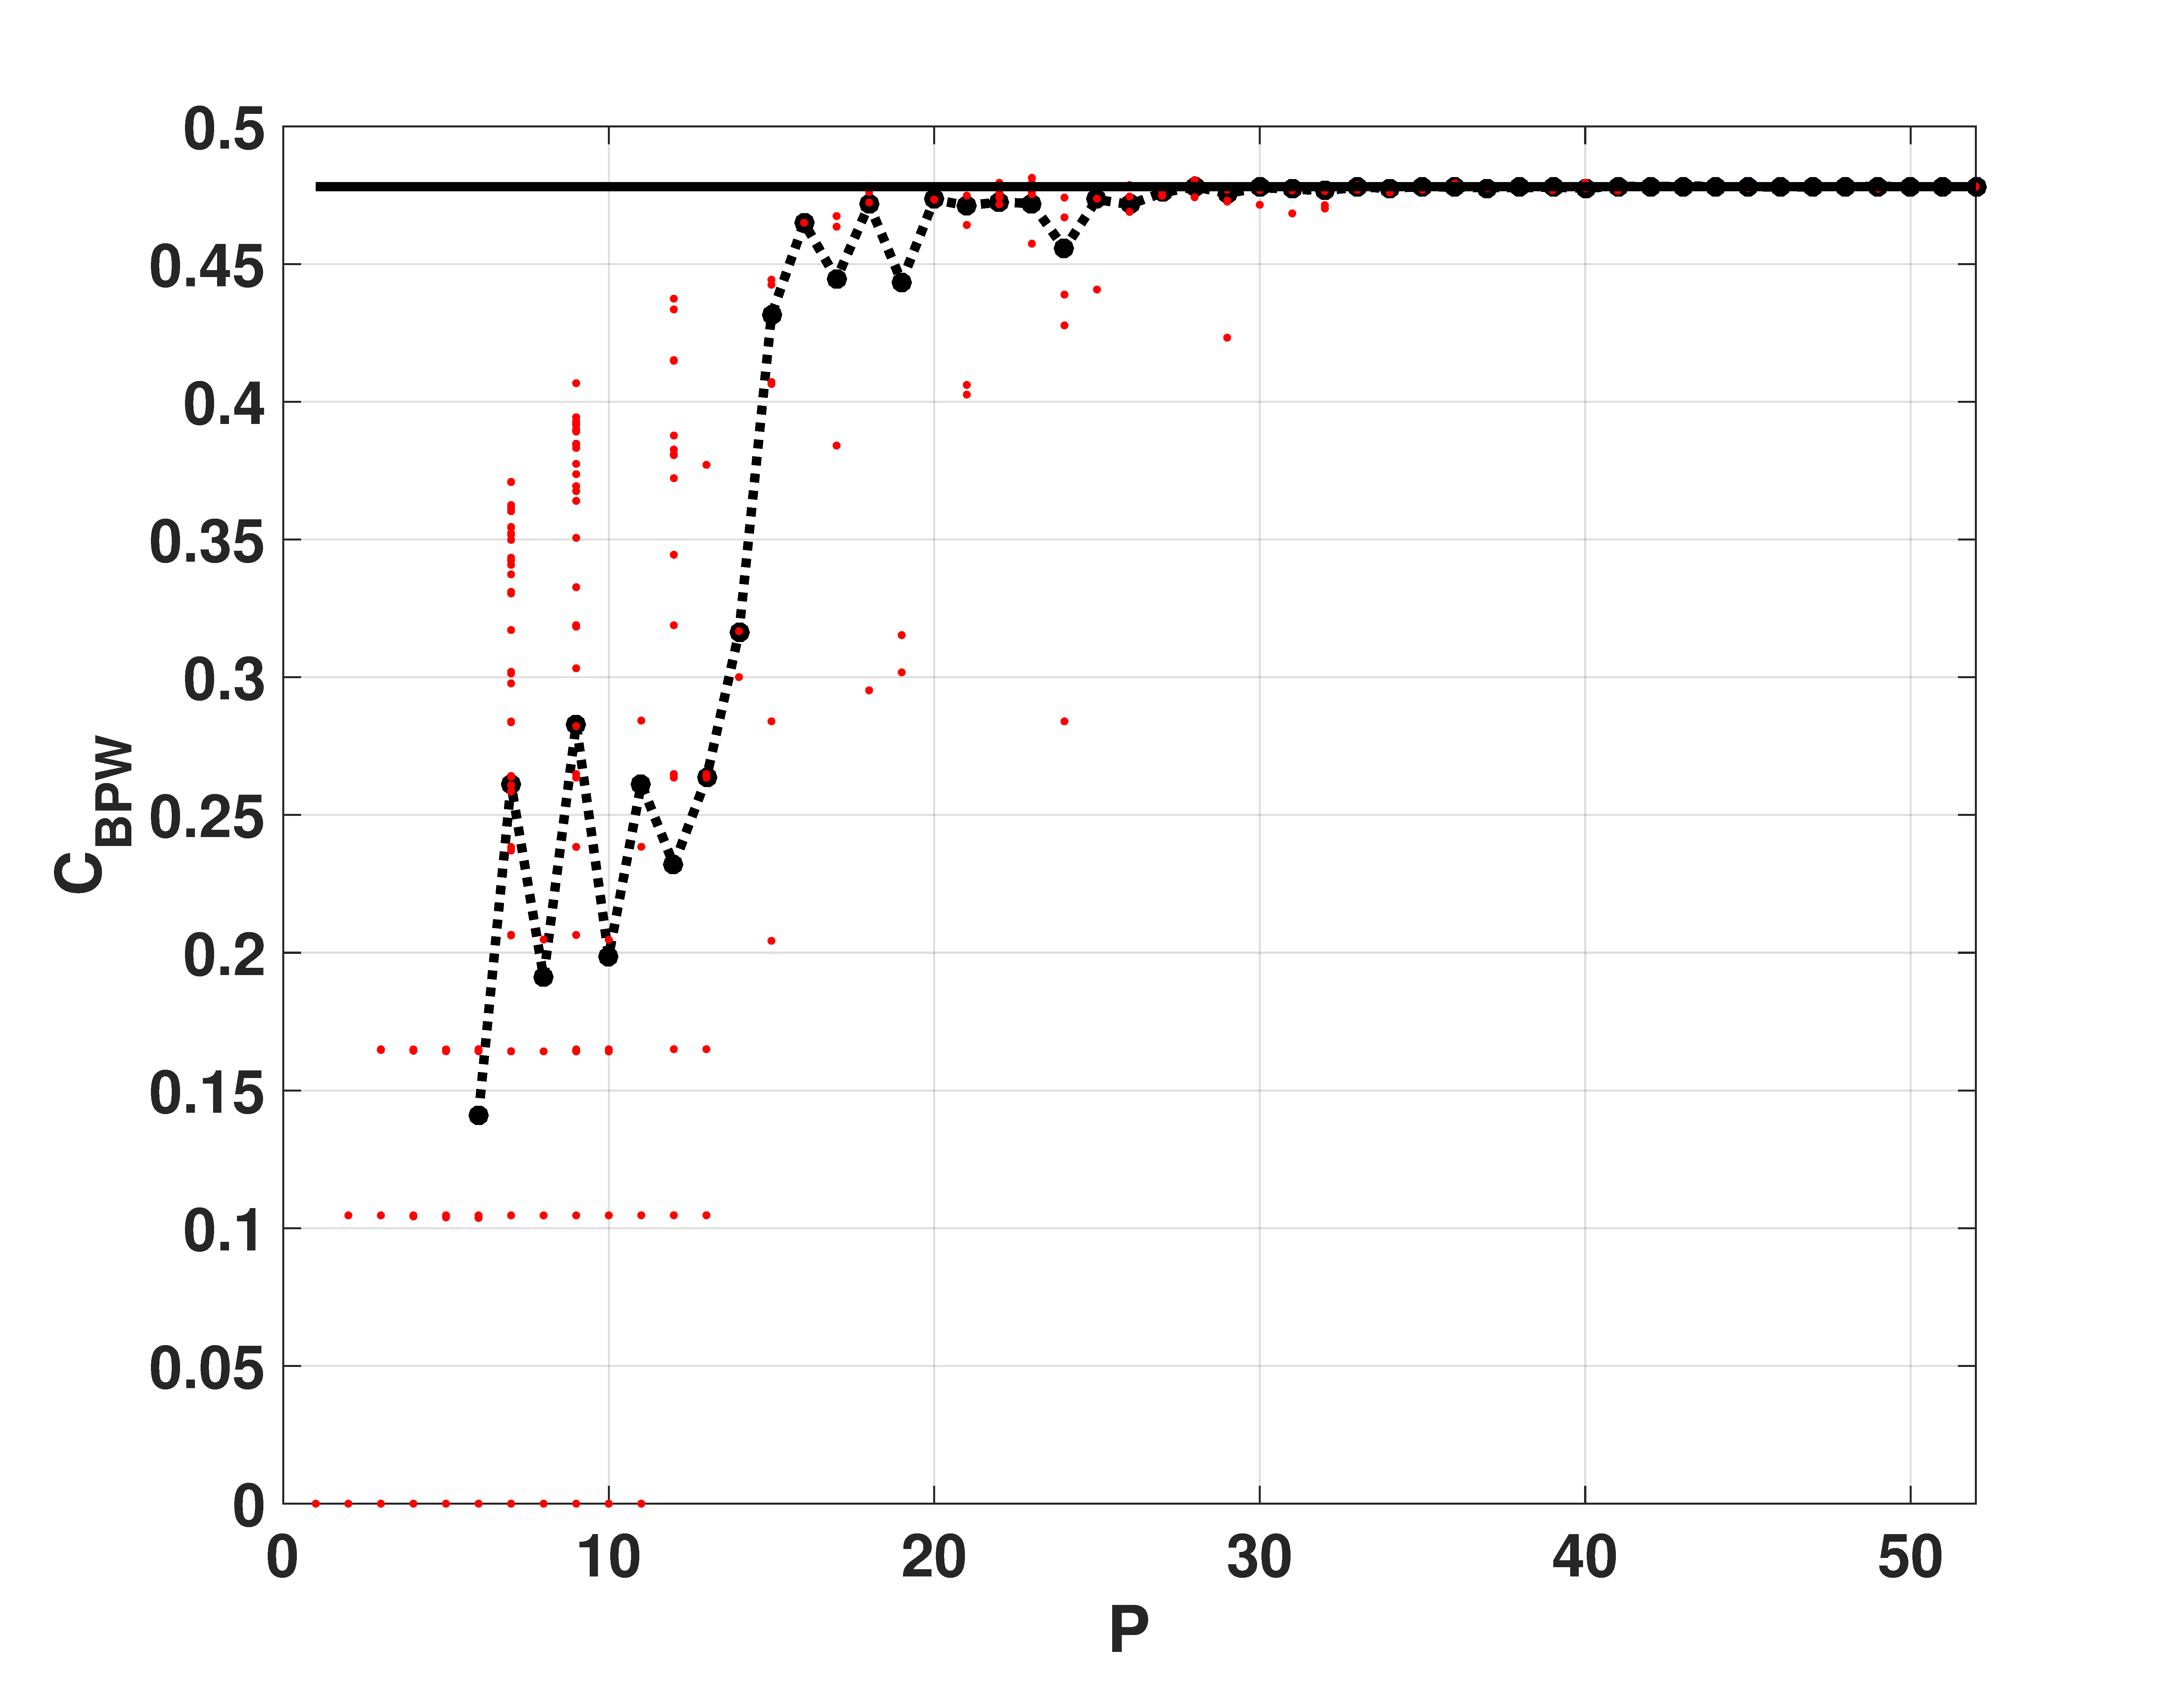
\includegraphics[width= .49\textwidth]{Cbpw_Log}
	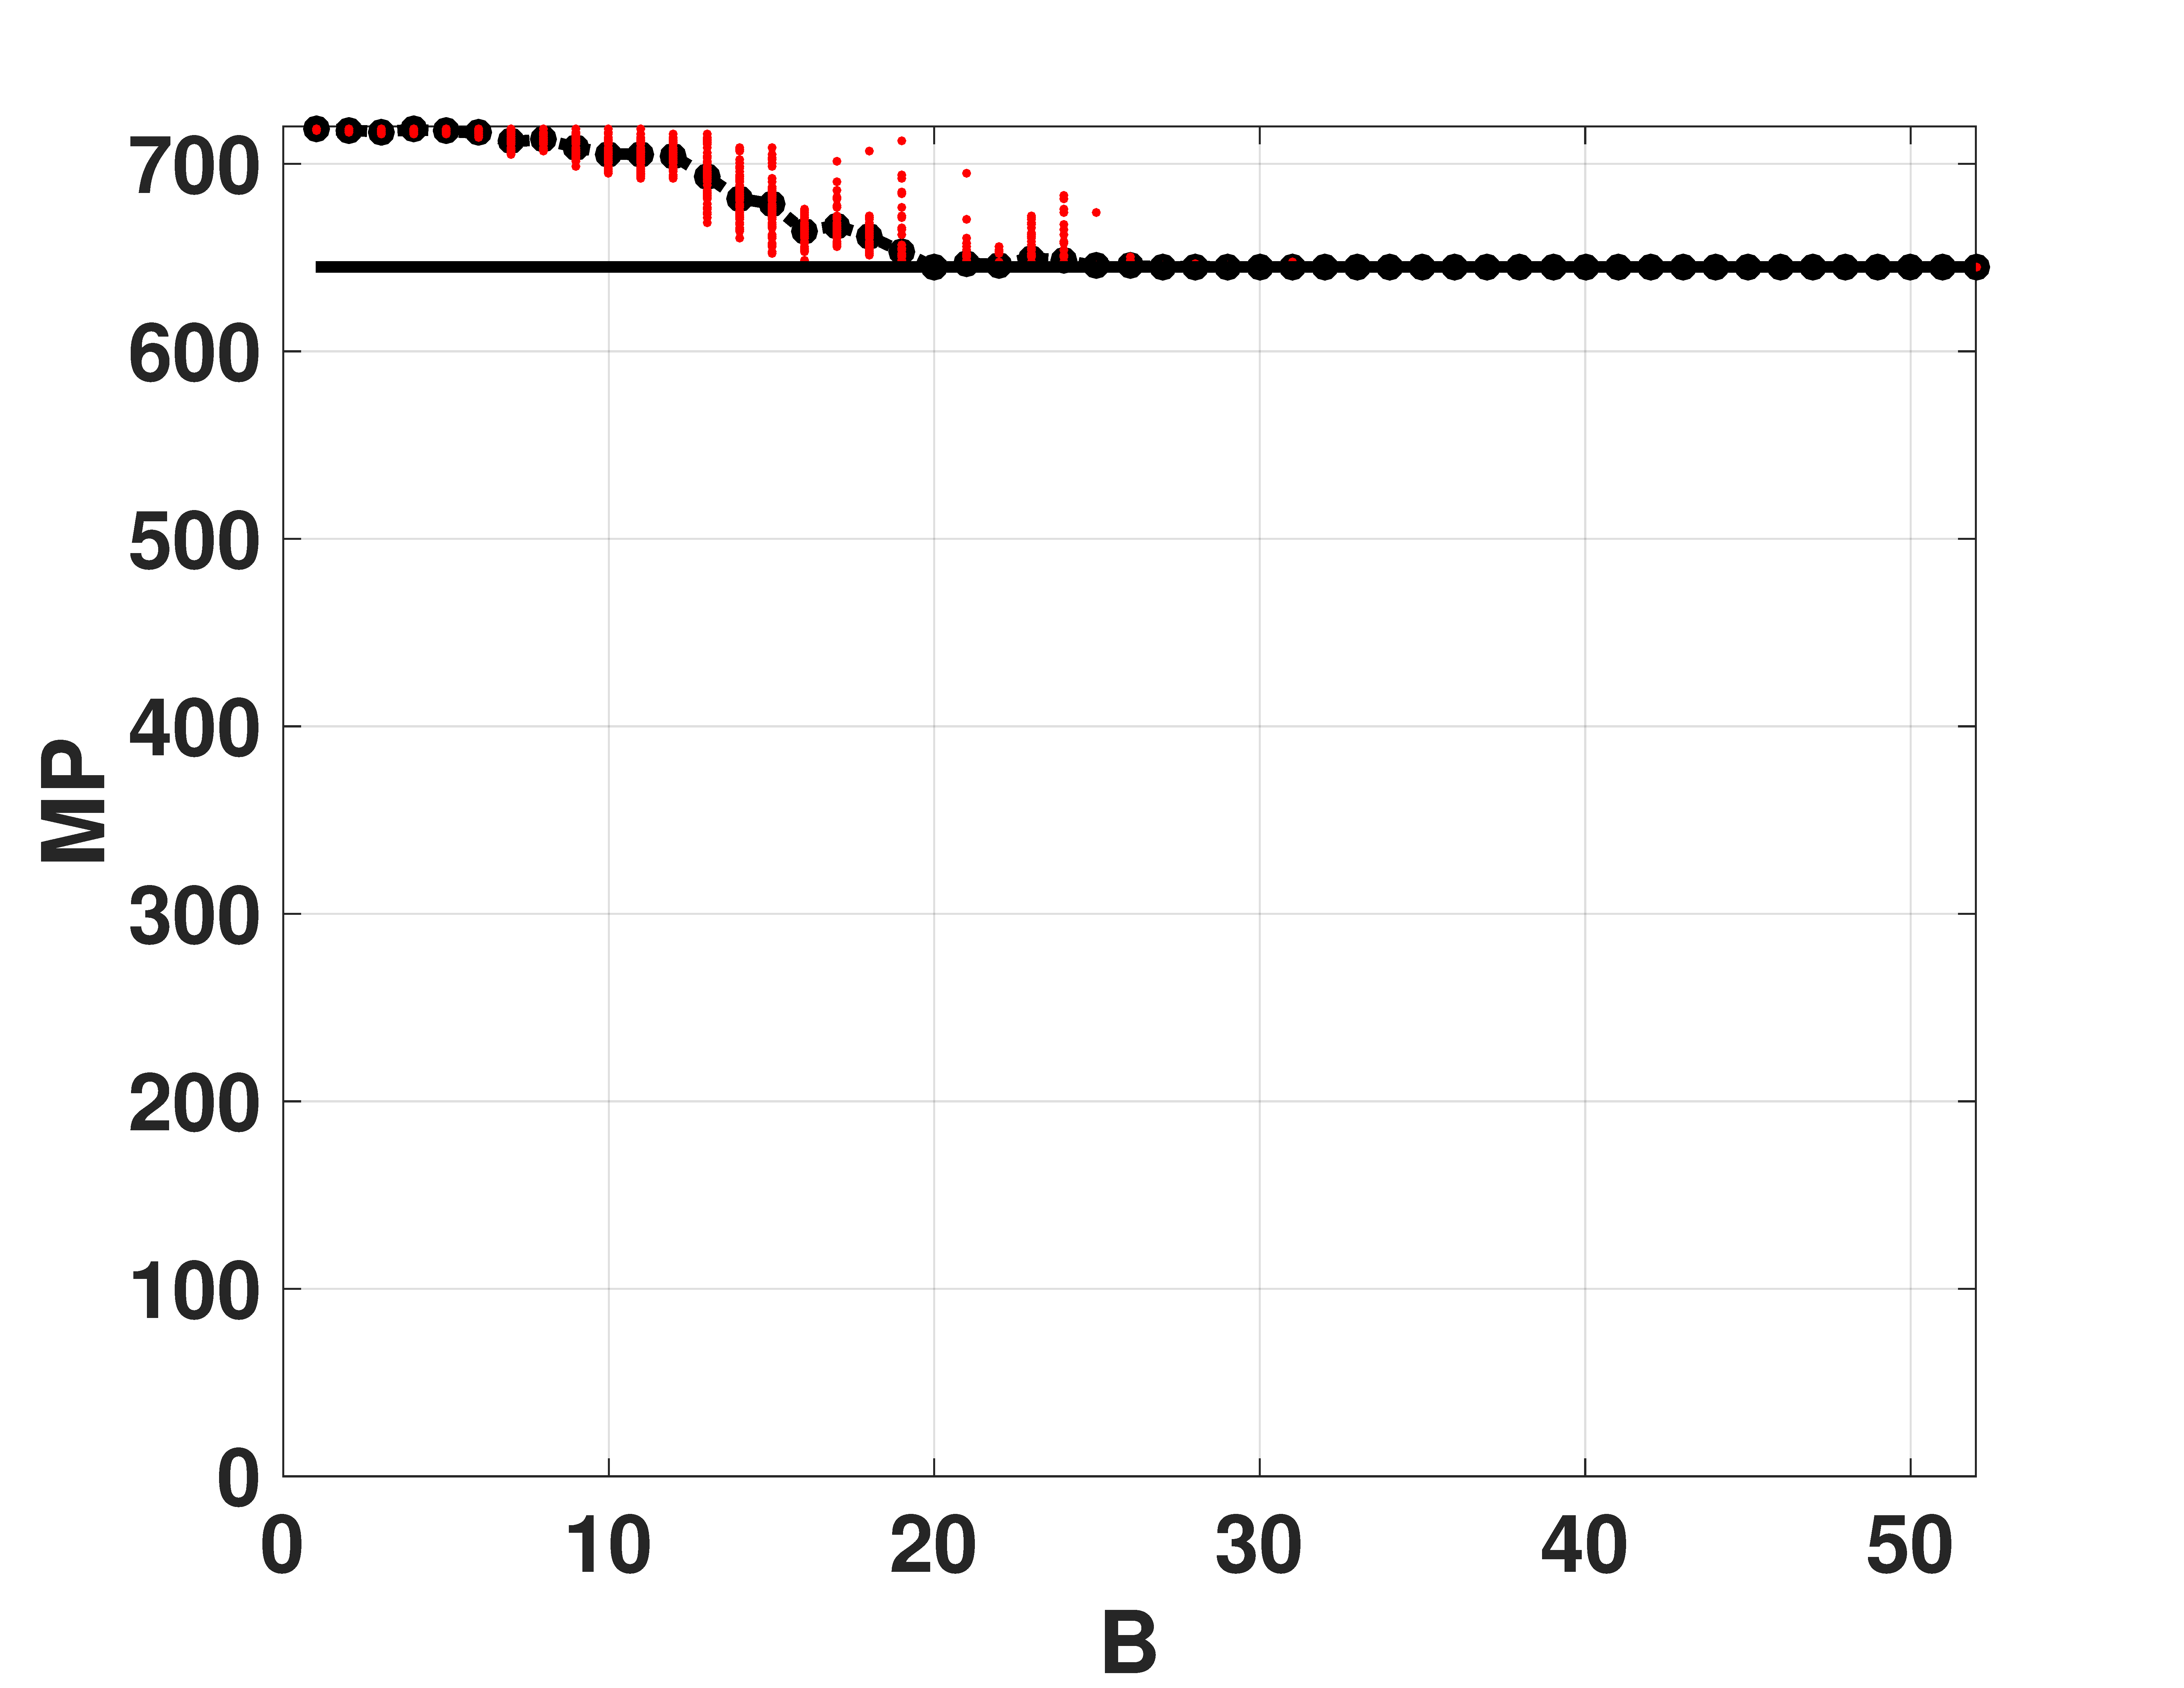
\includegraphics[width= .49\textwidth]{MP_Log}
	\caption{Statistical properties of the LOG map: (a) $H_{val}$ vs $B$ (b) $H_{BP}$ vs $B$ (c) $C_{BP}$ vs $B$ (d) $MP$ vs $B$.}
	\label{fig:LOG_QuantiB}
\end{figure}

The same results are now shown in double entropy planes with the precision as parameter (Fig. \ref{fig:LOG_HH}).
These figures show: $100$ red points for each fixed point precision ($B$) and in black their average (dashed black line connecting black dots), $100$ blue dots that are the results of each run in floating point and a black star their average.
This last $100$ points and their average are overlapped.

As expected, the fixed point architecture implementation converges to the floating point value as $B$ increases.
For both, Hbp-Hval and Hbpw-Hval, from $B=20$, $H_{val}$ improves but $H_{BP}$ remains constant.
It can be seen that the distribution of values reaches high values ($<H_{val}>=0.9669$) but their mixing is poor ($<H_{BP}>=0.6269$).

\begin{figure}
	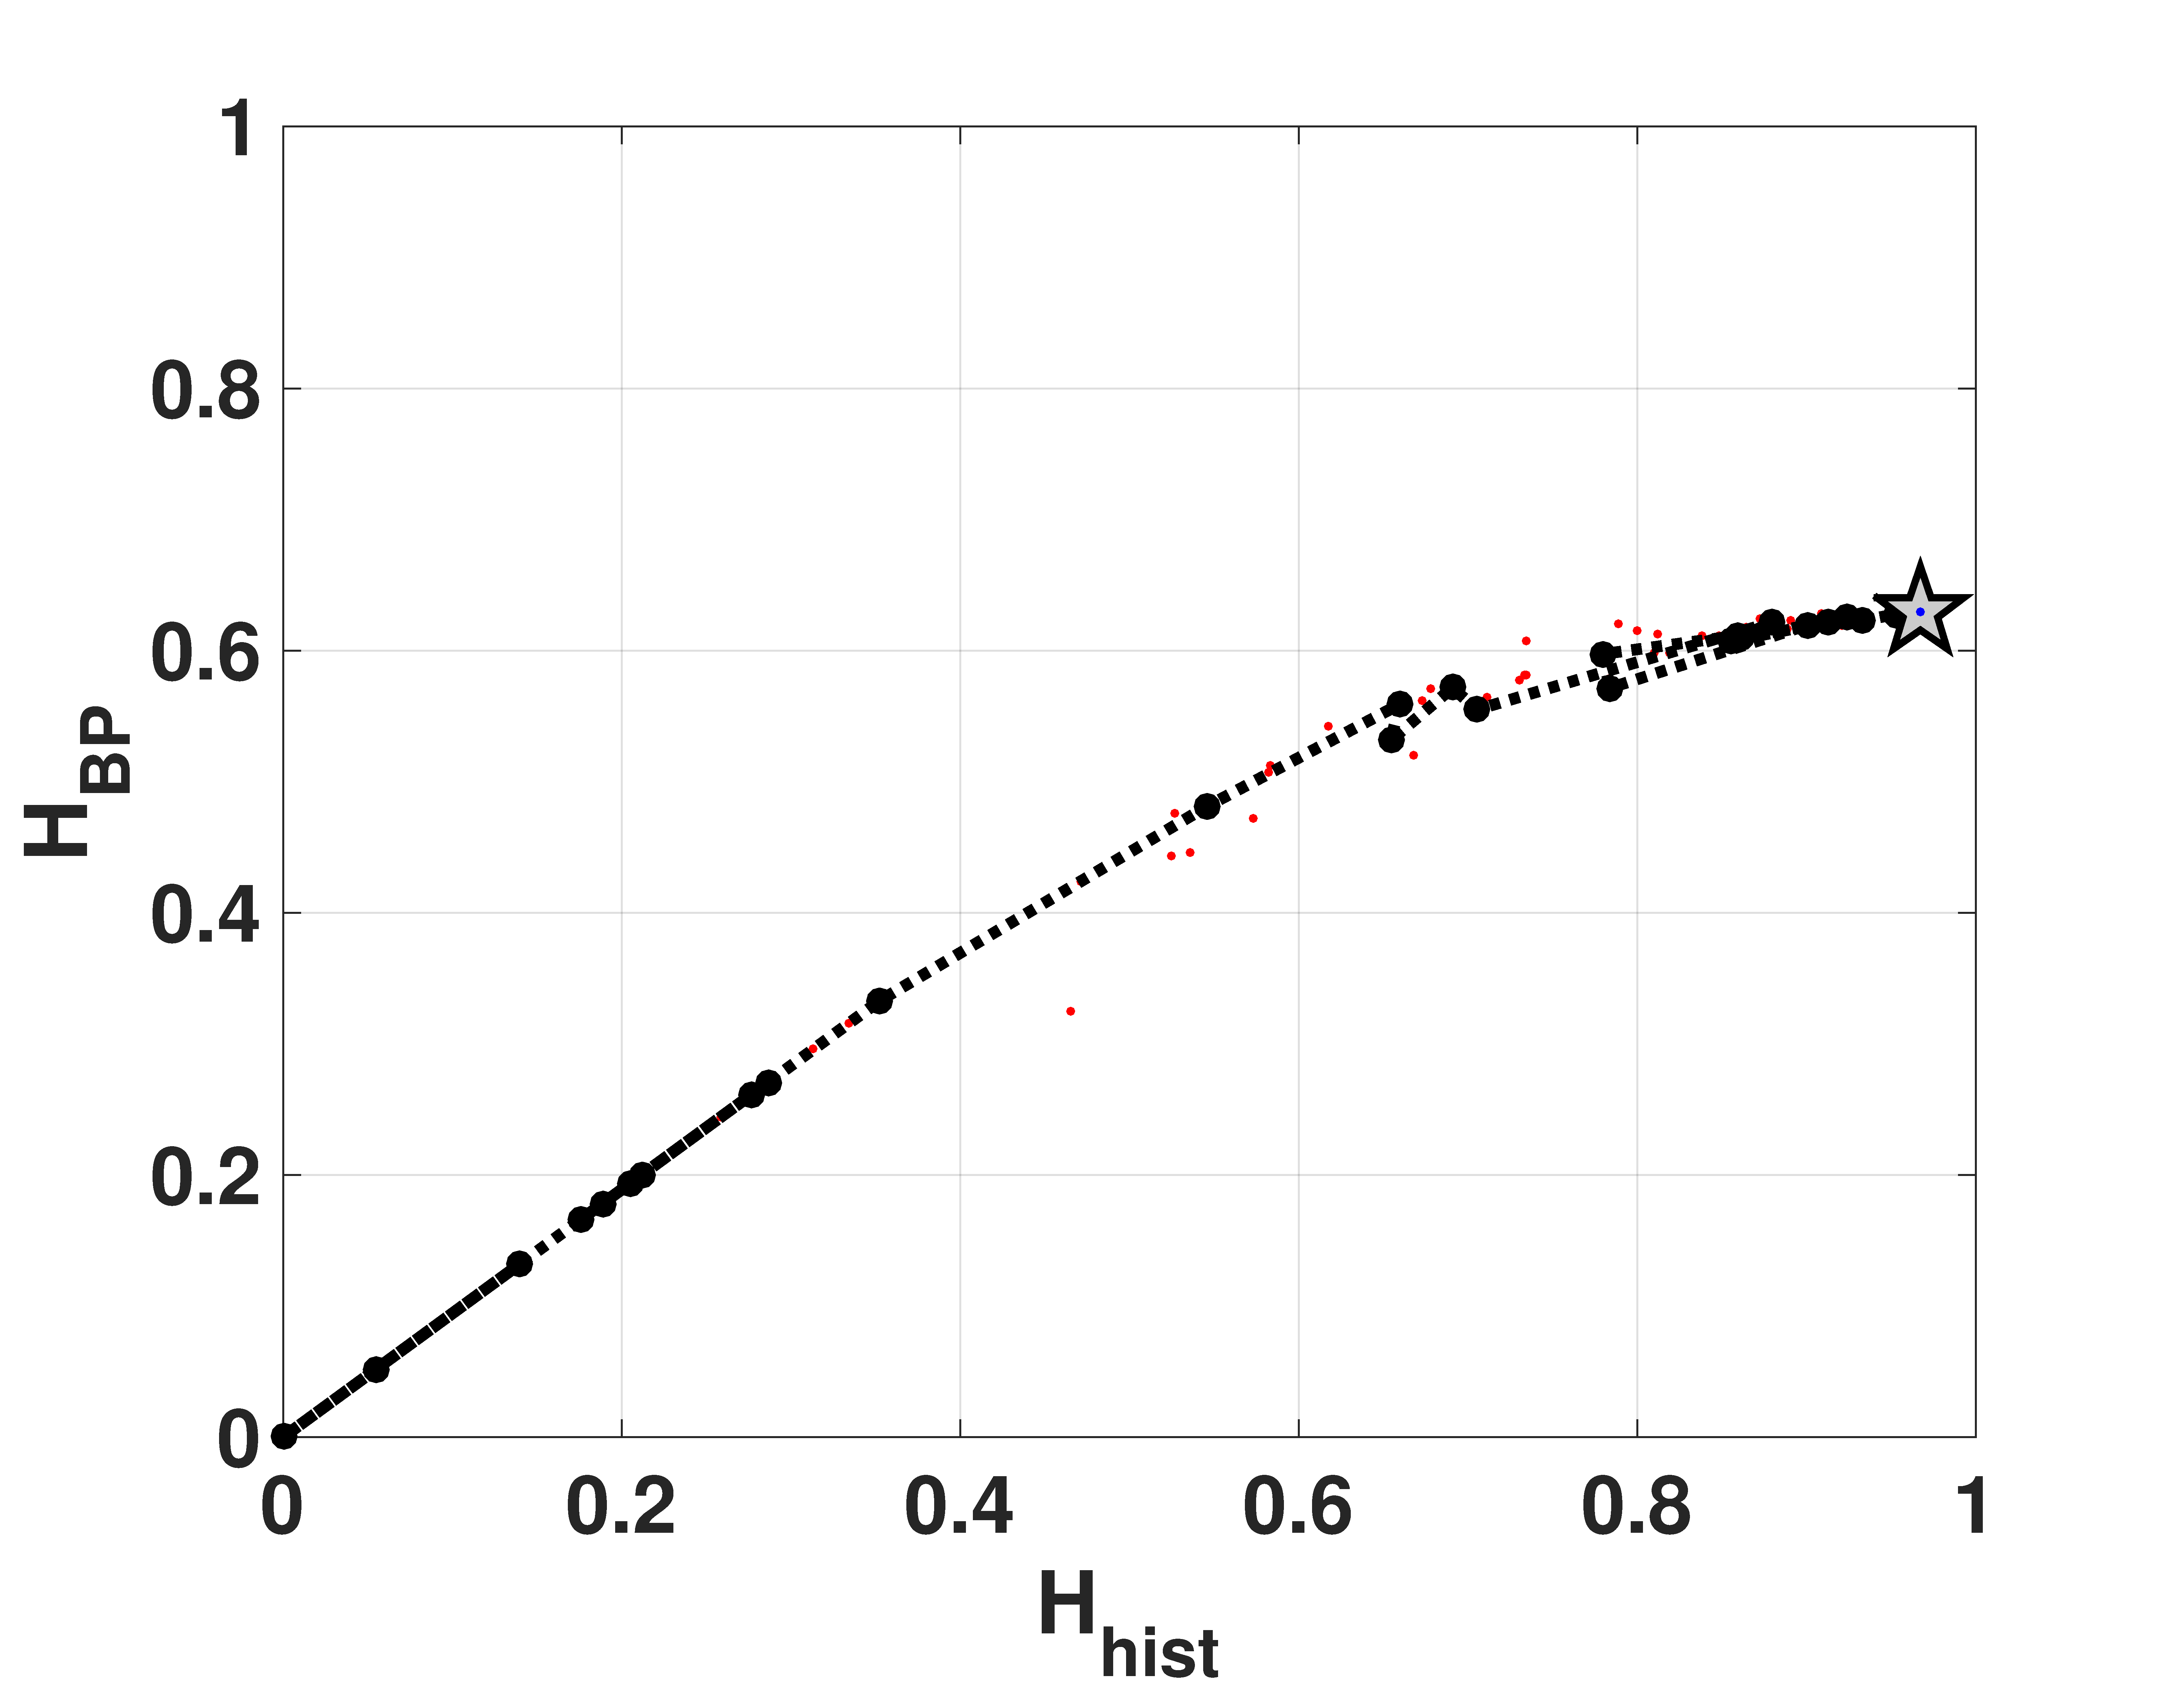
\includegraphics[width= .49\textwidth]{HbpHval_Log}
	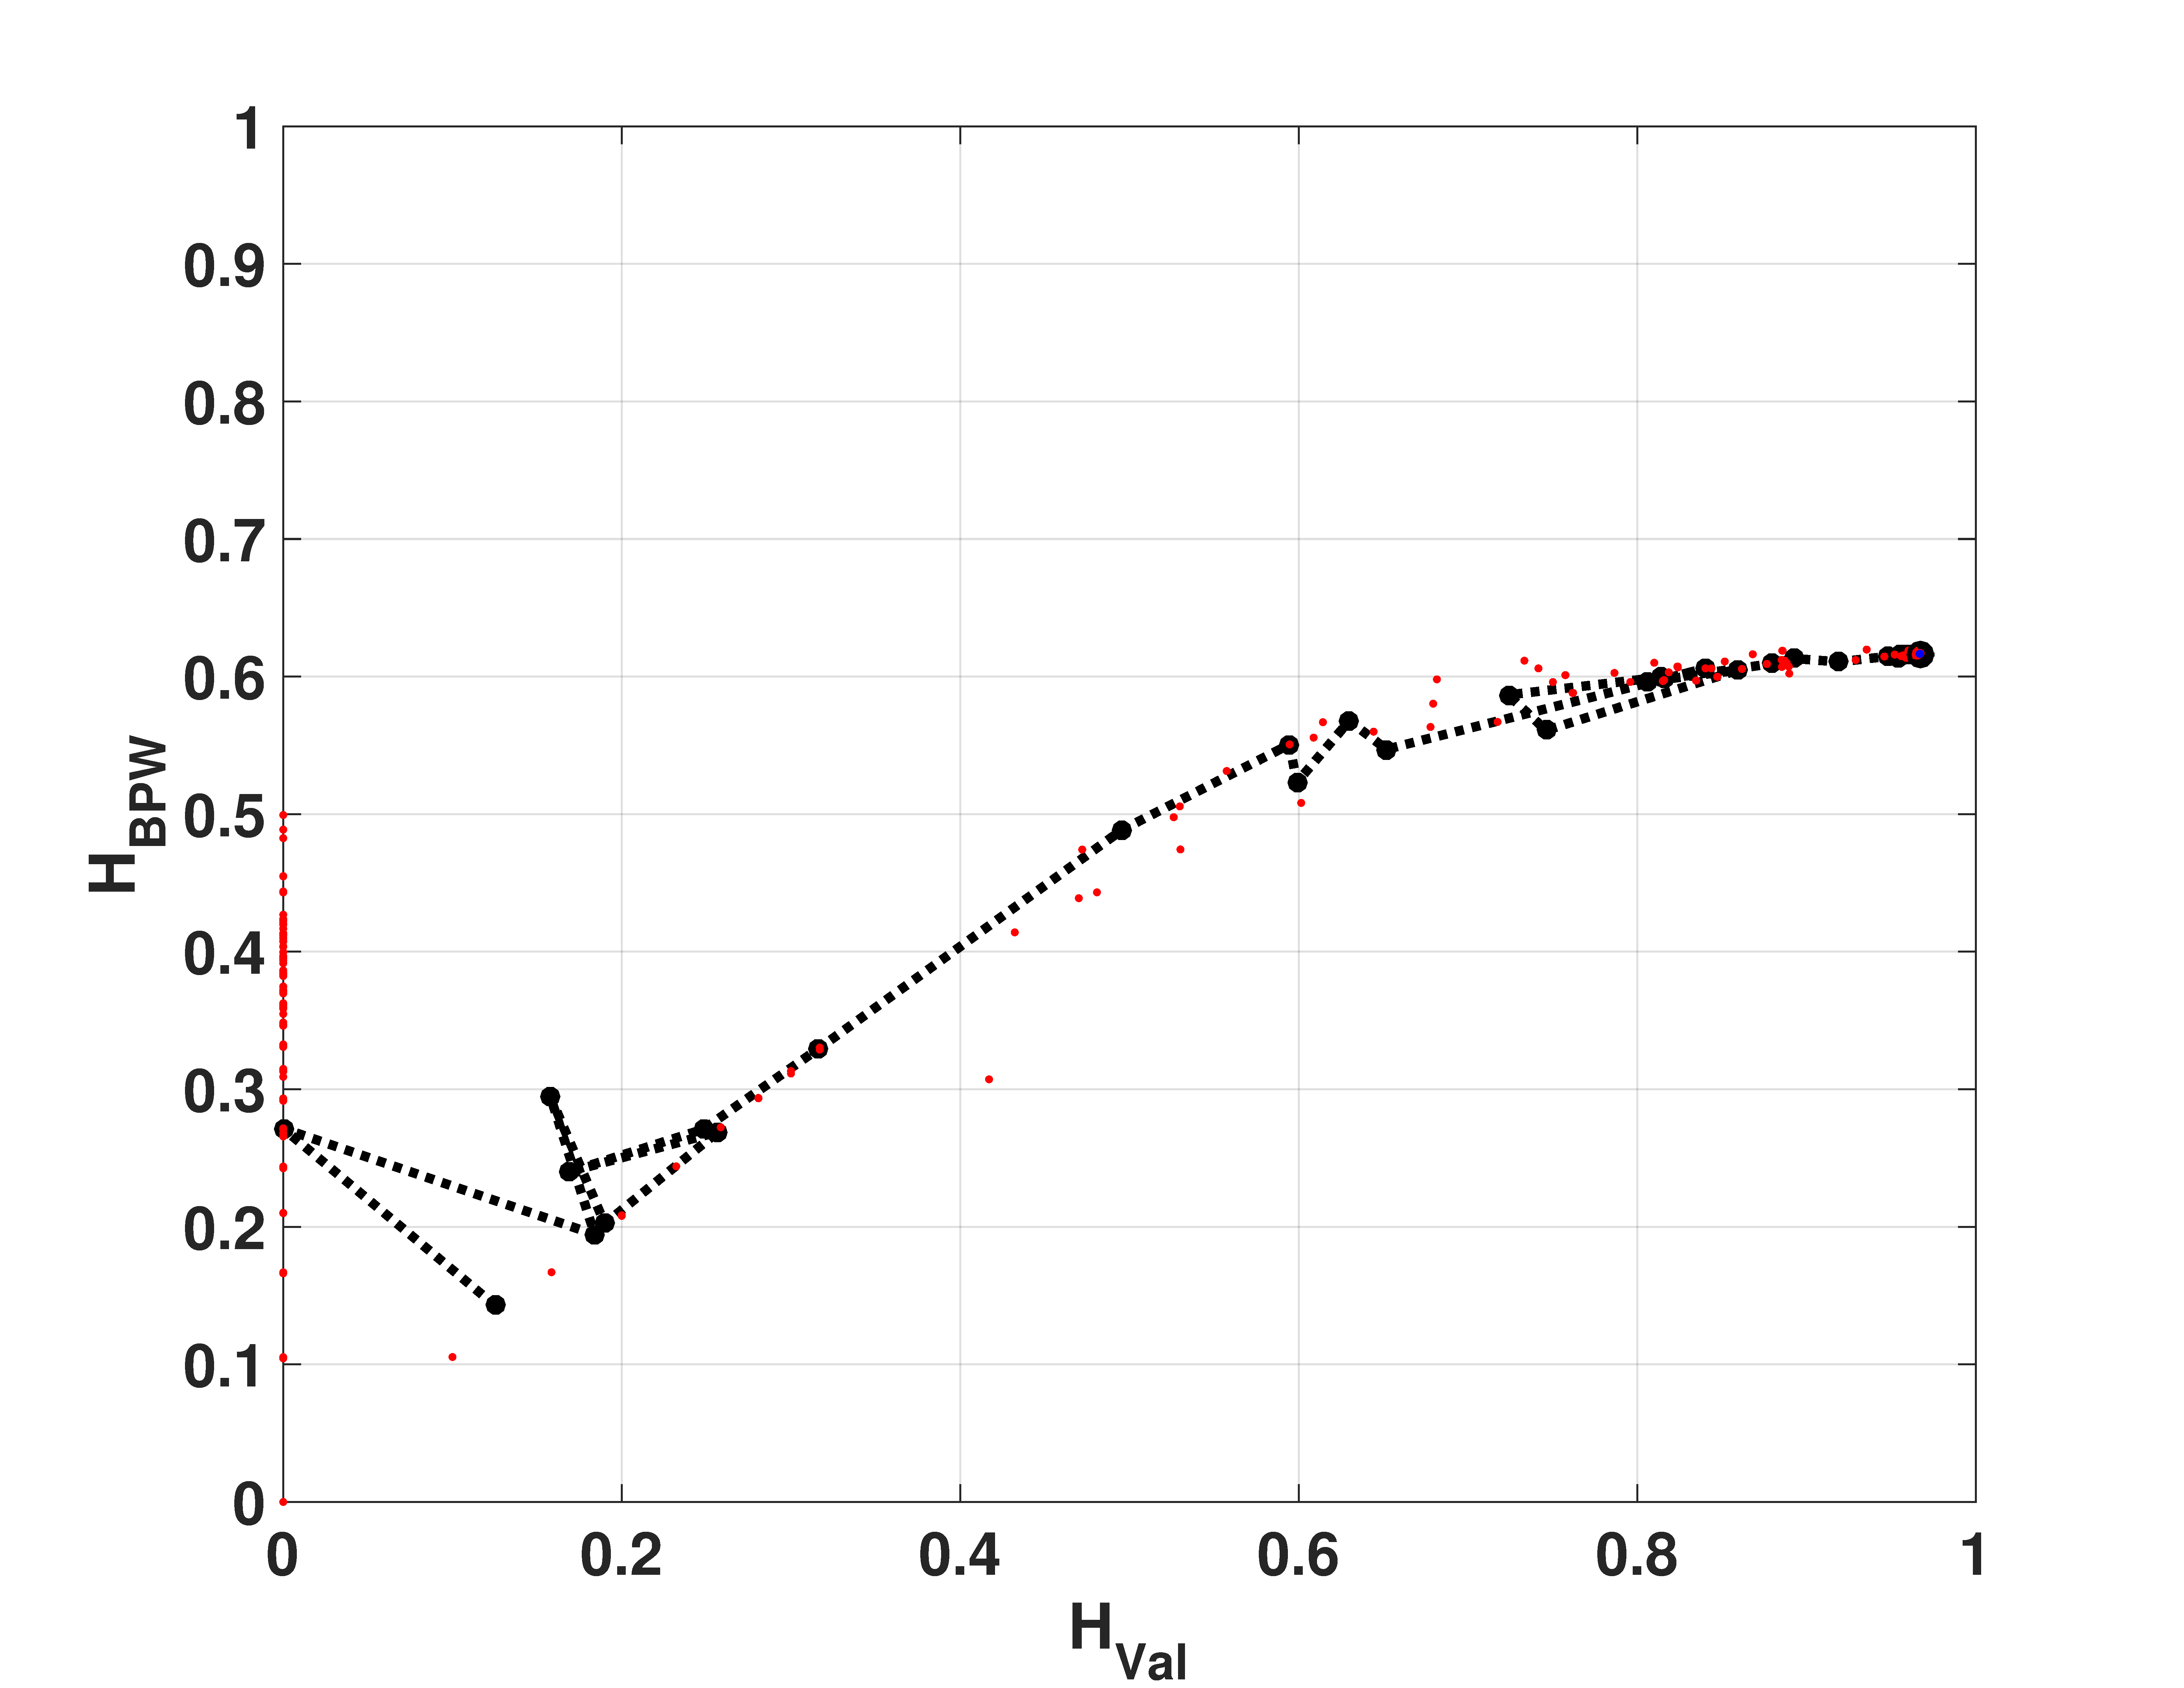
\includegraphics[width= .49\textwidth]{HbpwHval_Log}
	\caption{Evolution of statistical properties in double entropy plane of LOG map: (a) $H_{val}$ vs $H_{BP}$ (b) $H_{val}$ vs $H_{BPW}$.}
	\label{fig:LOG_HH}
\end{figure}

In Fig. \ref{fig:LOG_HC} we show the entropy-complexity planes.
Dotted gray lines are the upper and lower margins, is expected that a chaotic system remains near the upper margin.
These results characterize a chaotic behaviour, in $H_{BP}-C_{BP}$ plane we can see a low entropy and high complexity.

\begin{figure}
	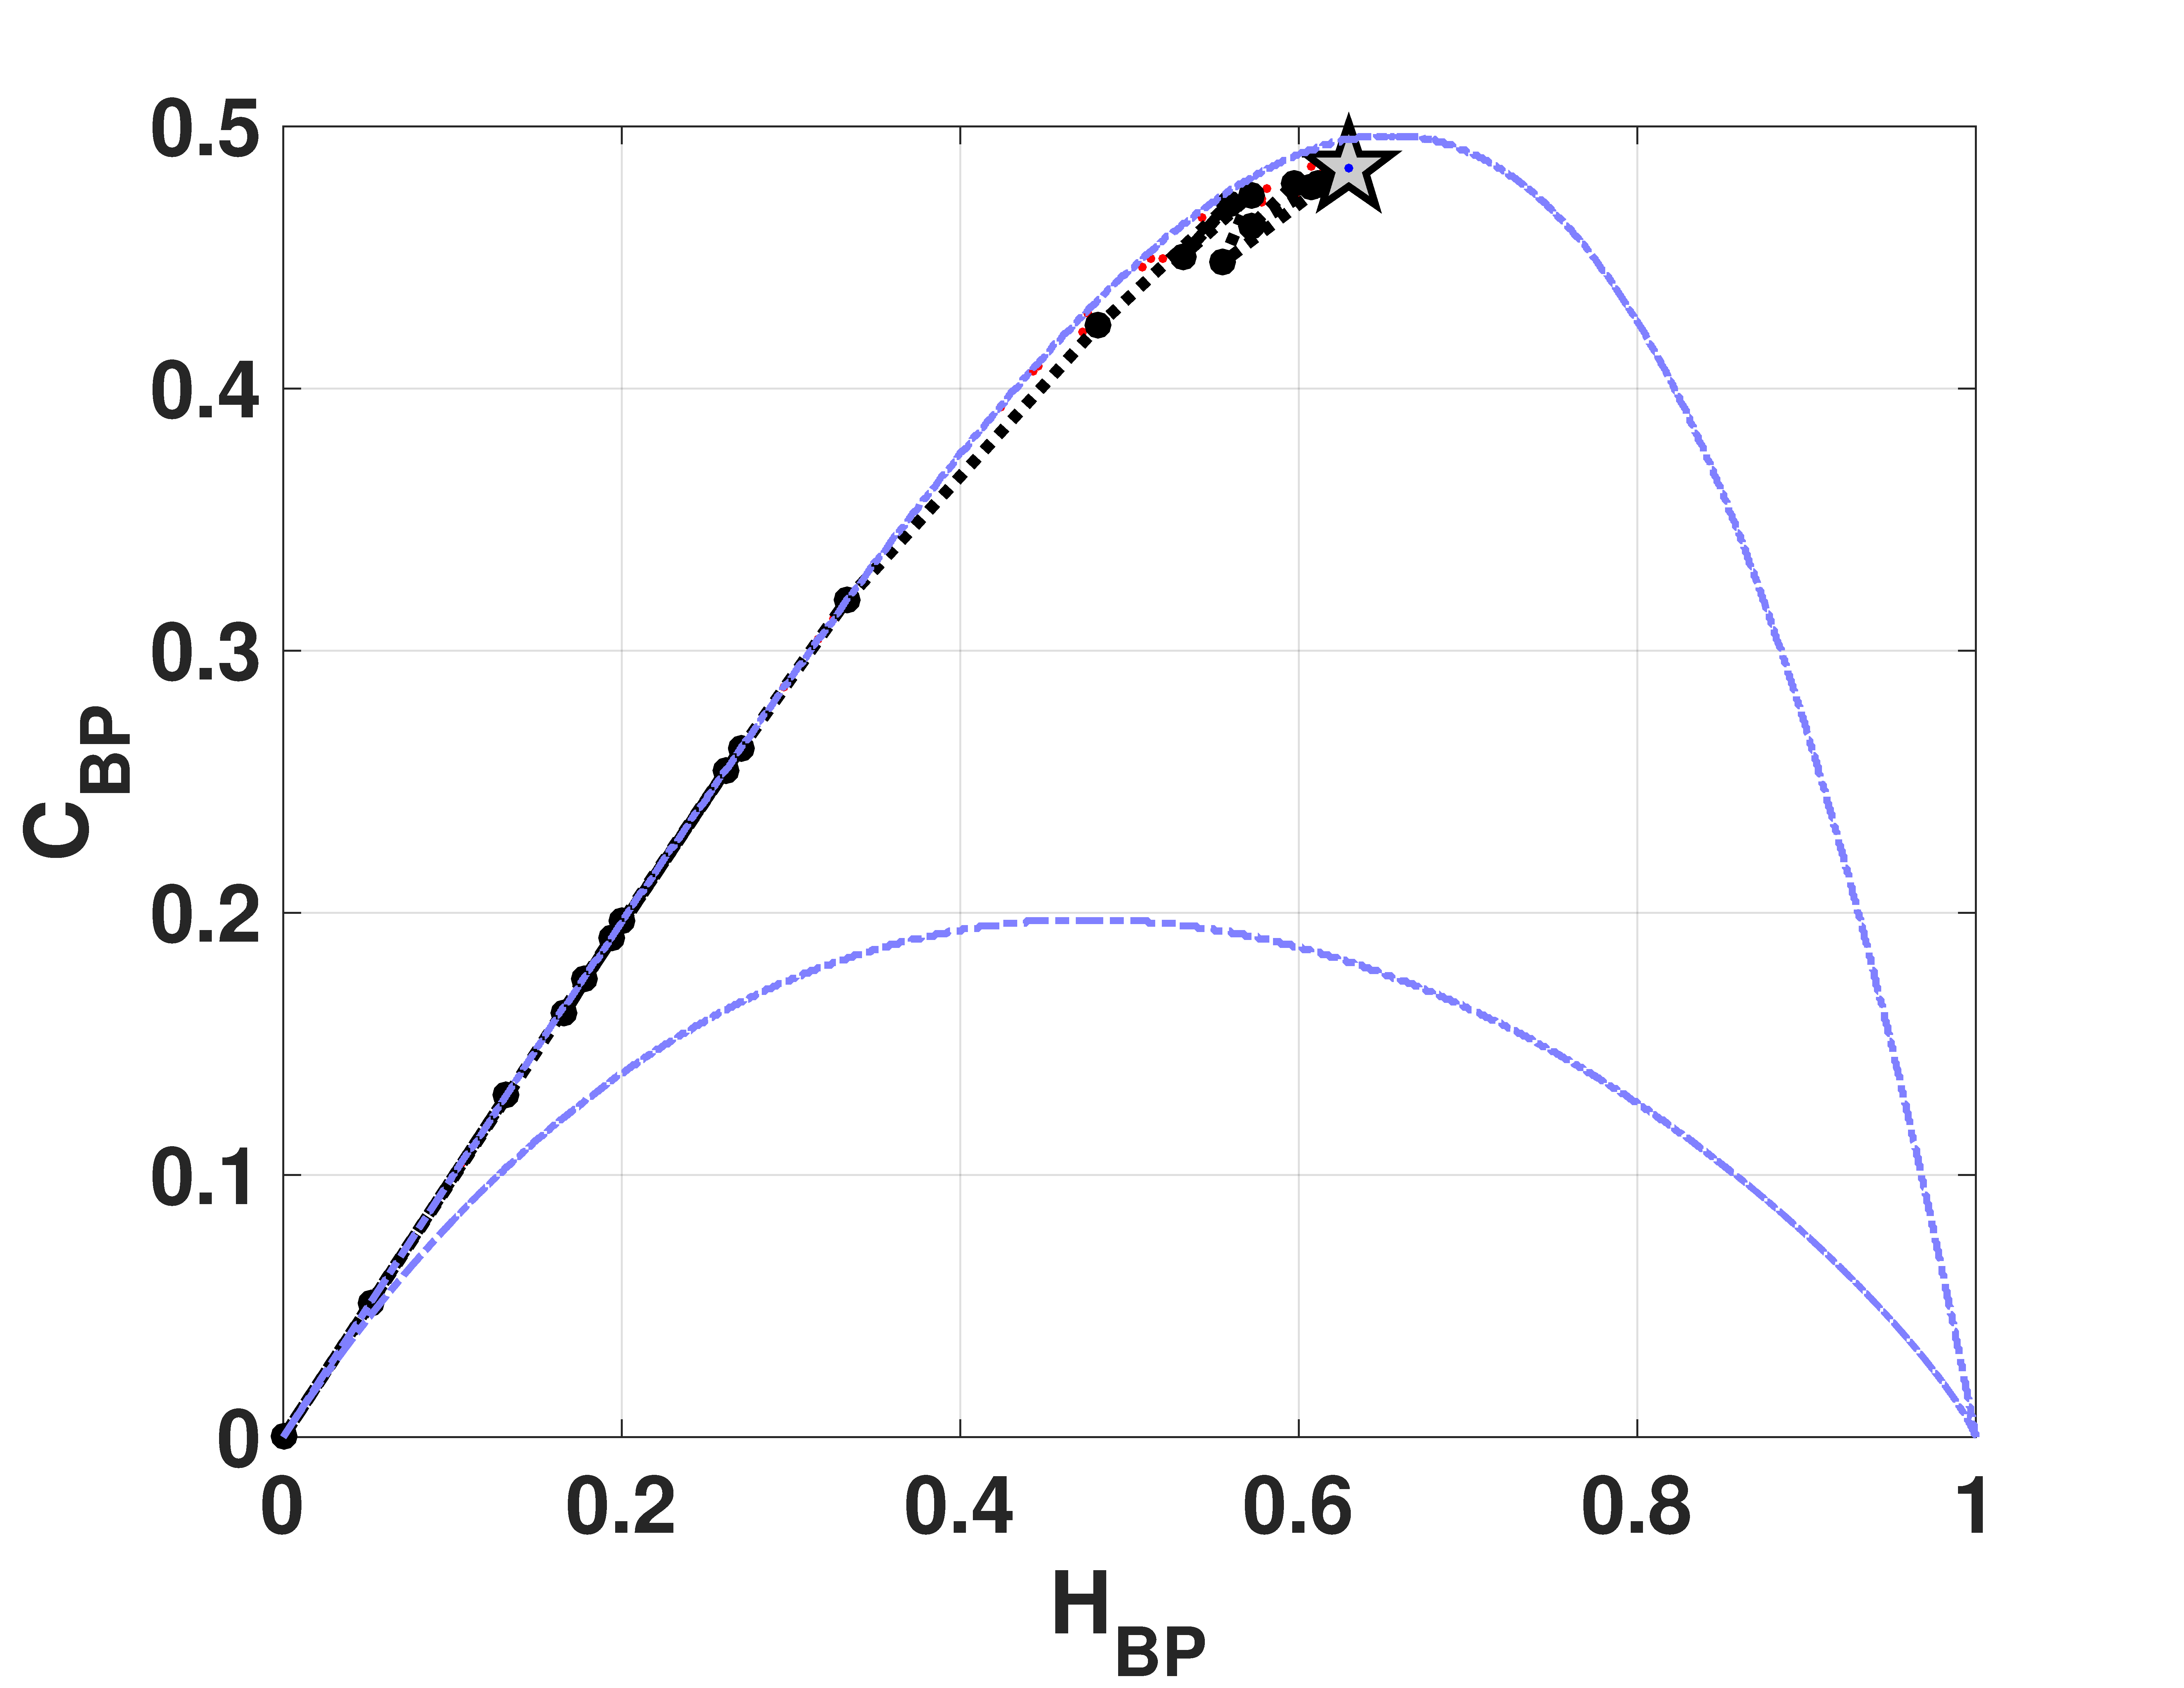
\includegraphics[width= .49\textwidth]{CbpHbp_Log}
	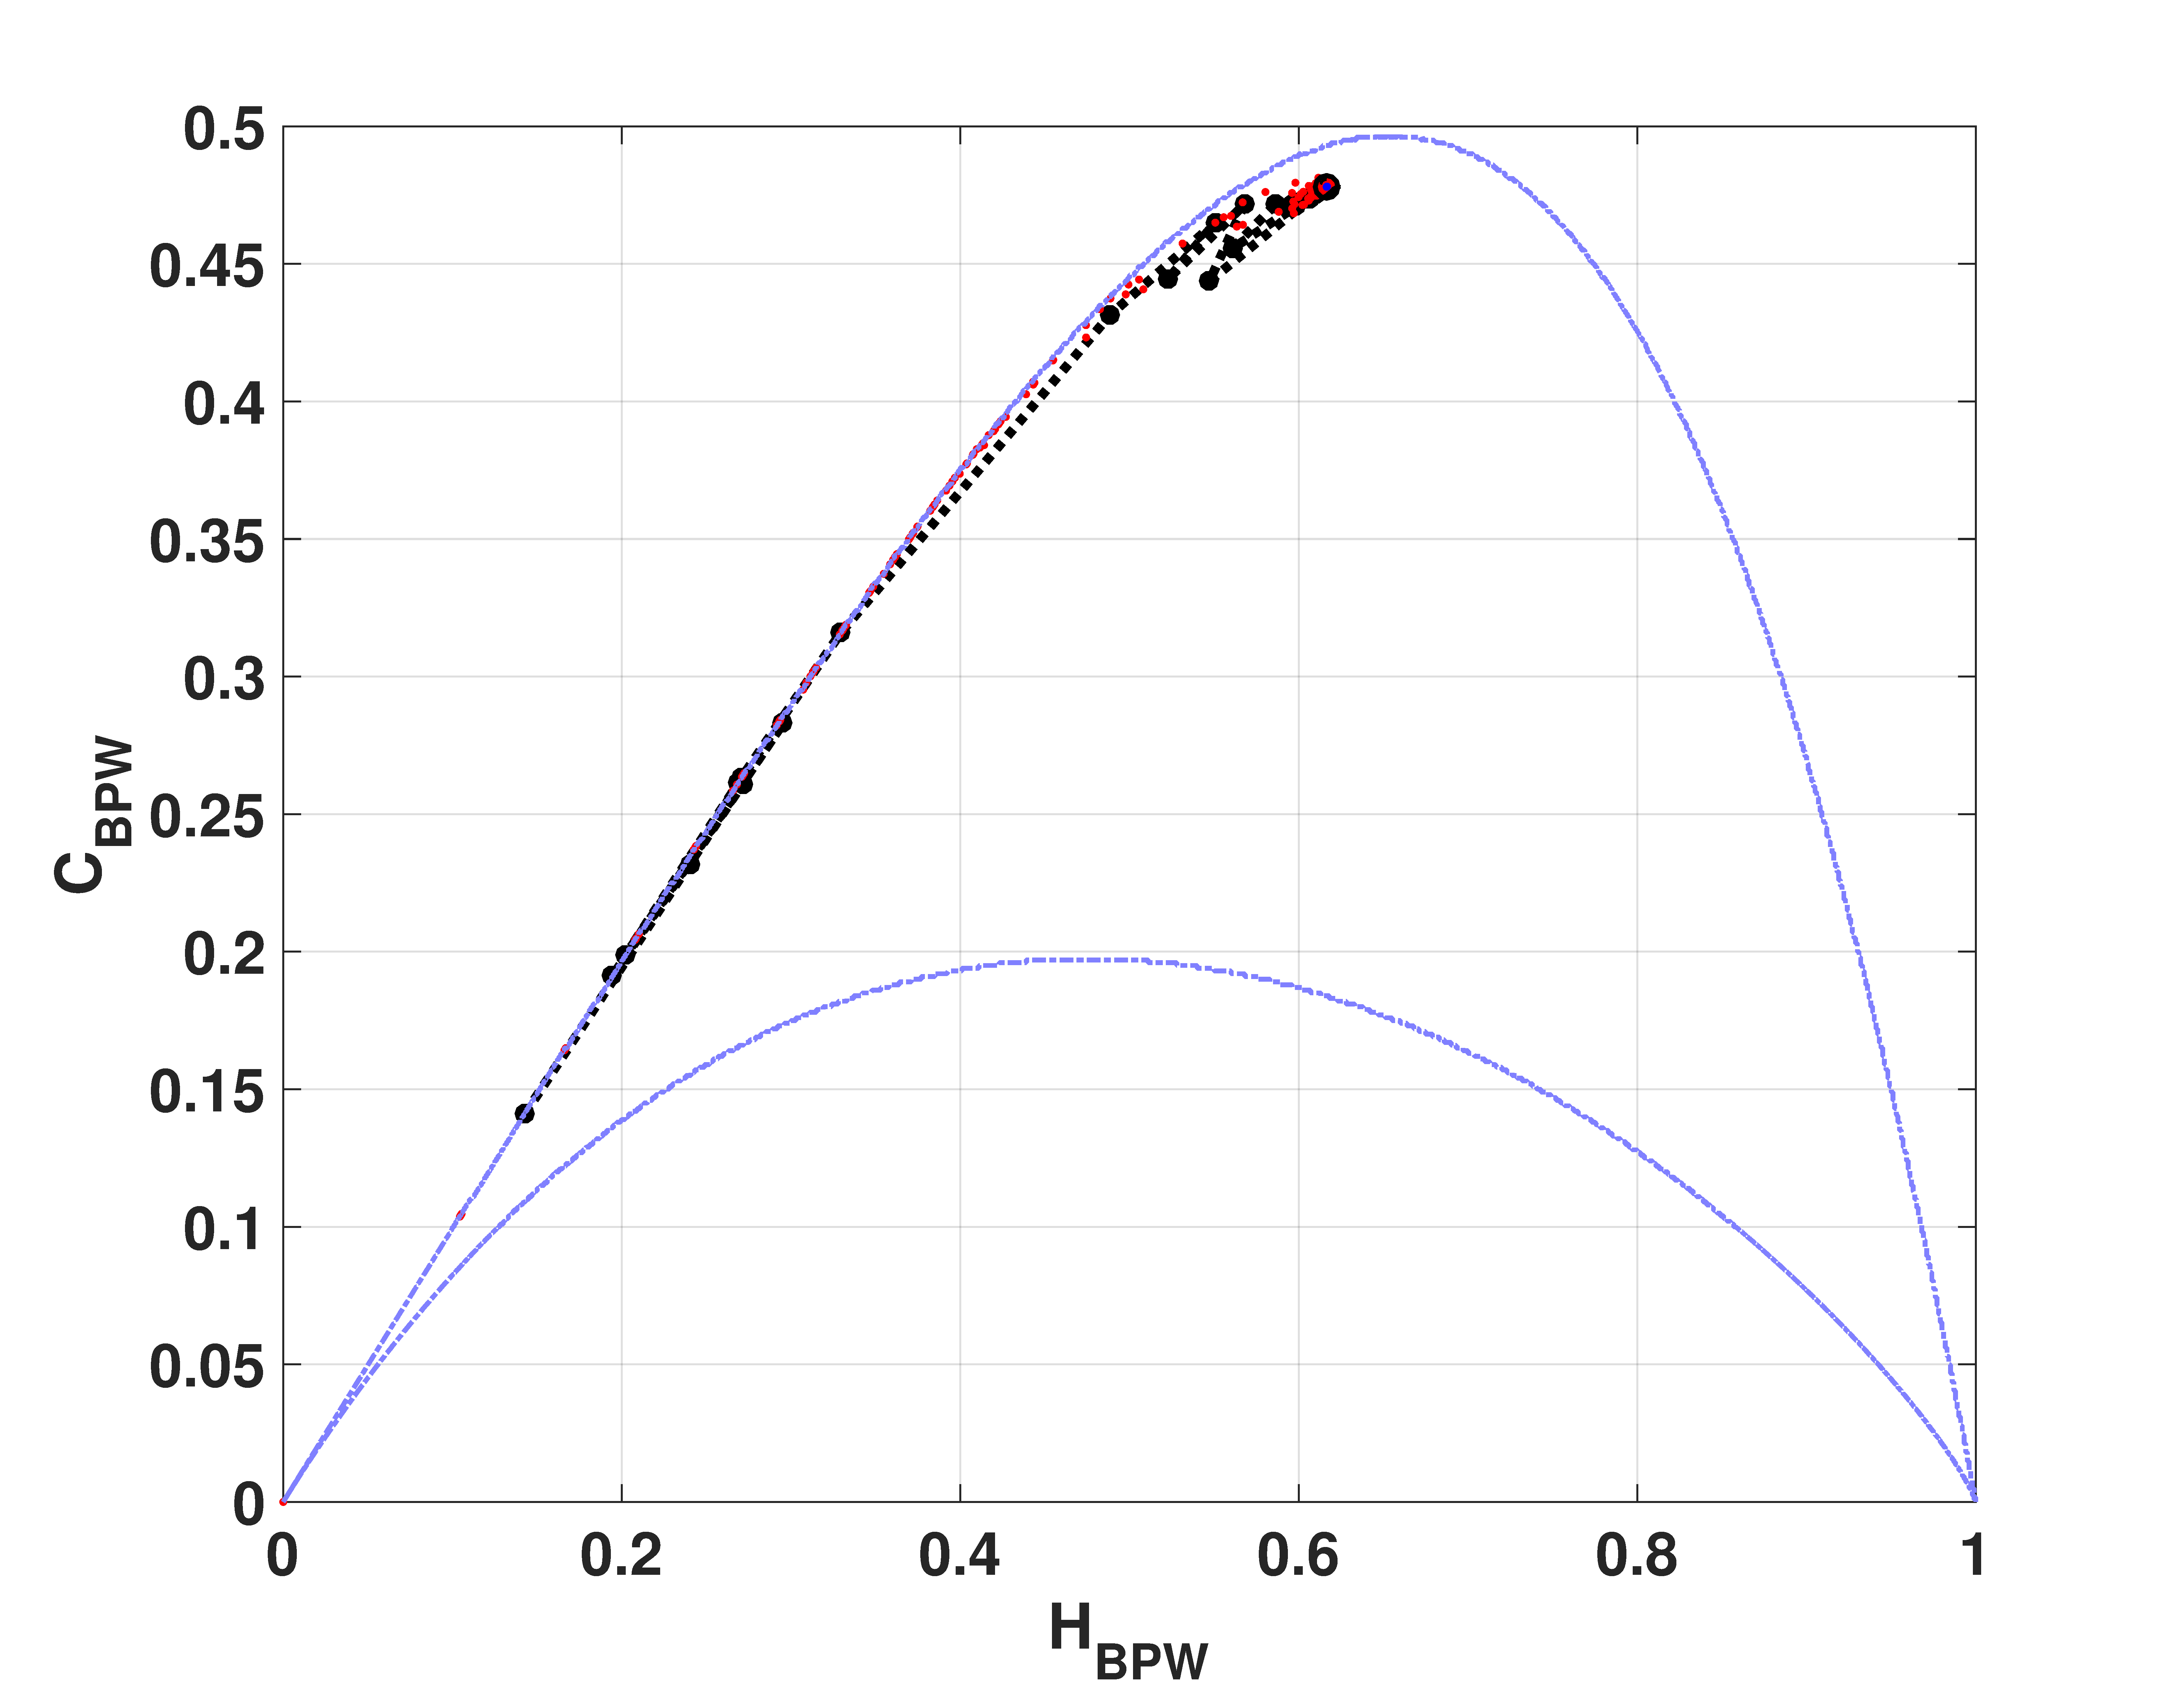
\includegraphics[width= .49\textwidth]{CbpwHbpw_Log}
	\caption{Evolution of statistical properties in entropy-complexity plane of LOG map: (a) $C_{BP}$ vs $H_{BP}$ (b) $C_{BPW}$ vs $H_{BPW}$.}
	\label{fig:LOG_HC}
\end{figure}


\subsubsection{TENT} \label{sssec:tent}

When this map is implemented in a computer using any numerical representation system (even floating-point!) truncation errors rapidly increase and make unstable fixed point in $x^*=0$ to become stable.
The sequences within the attractor domain of this fixed point will have a short transitory of length between $0$ and $B$ followed by an infinite number of $0$'s \cite{Jessa2002,Callegari}.
This issue is easily explained in \cite{Li2004}, the problem appears because all iterations have a left-shift operation that carries the $0$'s from the right side of the number to the most significant positions.

Figs. \ref{fig:Hval_Tent} to \ref{fig:MP_Tent} show the quantifiers for floating- and fixed-point numerical representations.
Quantifiers $H_{hist}$, $H_{BP}$ and $C_{BP}$ are equal to zero for all precisions, this reflects that the series quickly converge toward a fixed point for all sequences.
In the case of $H_{BPW}$ and $C_{BPW}$ quantifiers are different to non-null because BPW procedure discards the elements once they reach the fixed point.
The high dispersions in $H_{BPW}$, $C_{BPW}$ and MP are related to the short length of series transient.
These transients that converge to a fixed point have a maximum length of $B$ iterations for fixed-point arithmetic and $80$ for floating-point (long double precision).

\begin{figure}[htpb]
	\centering
	\begin{subfigure}[b]{0.49\textwidth}
		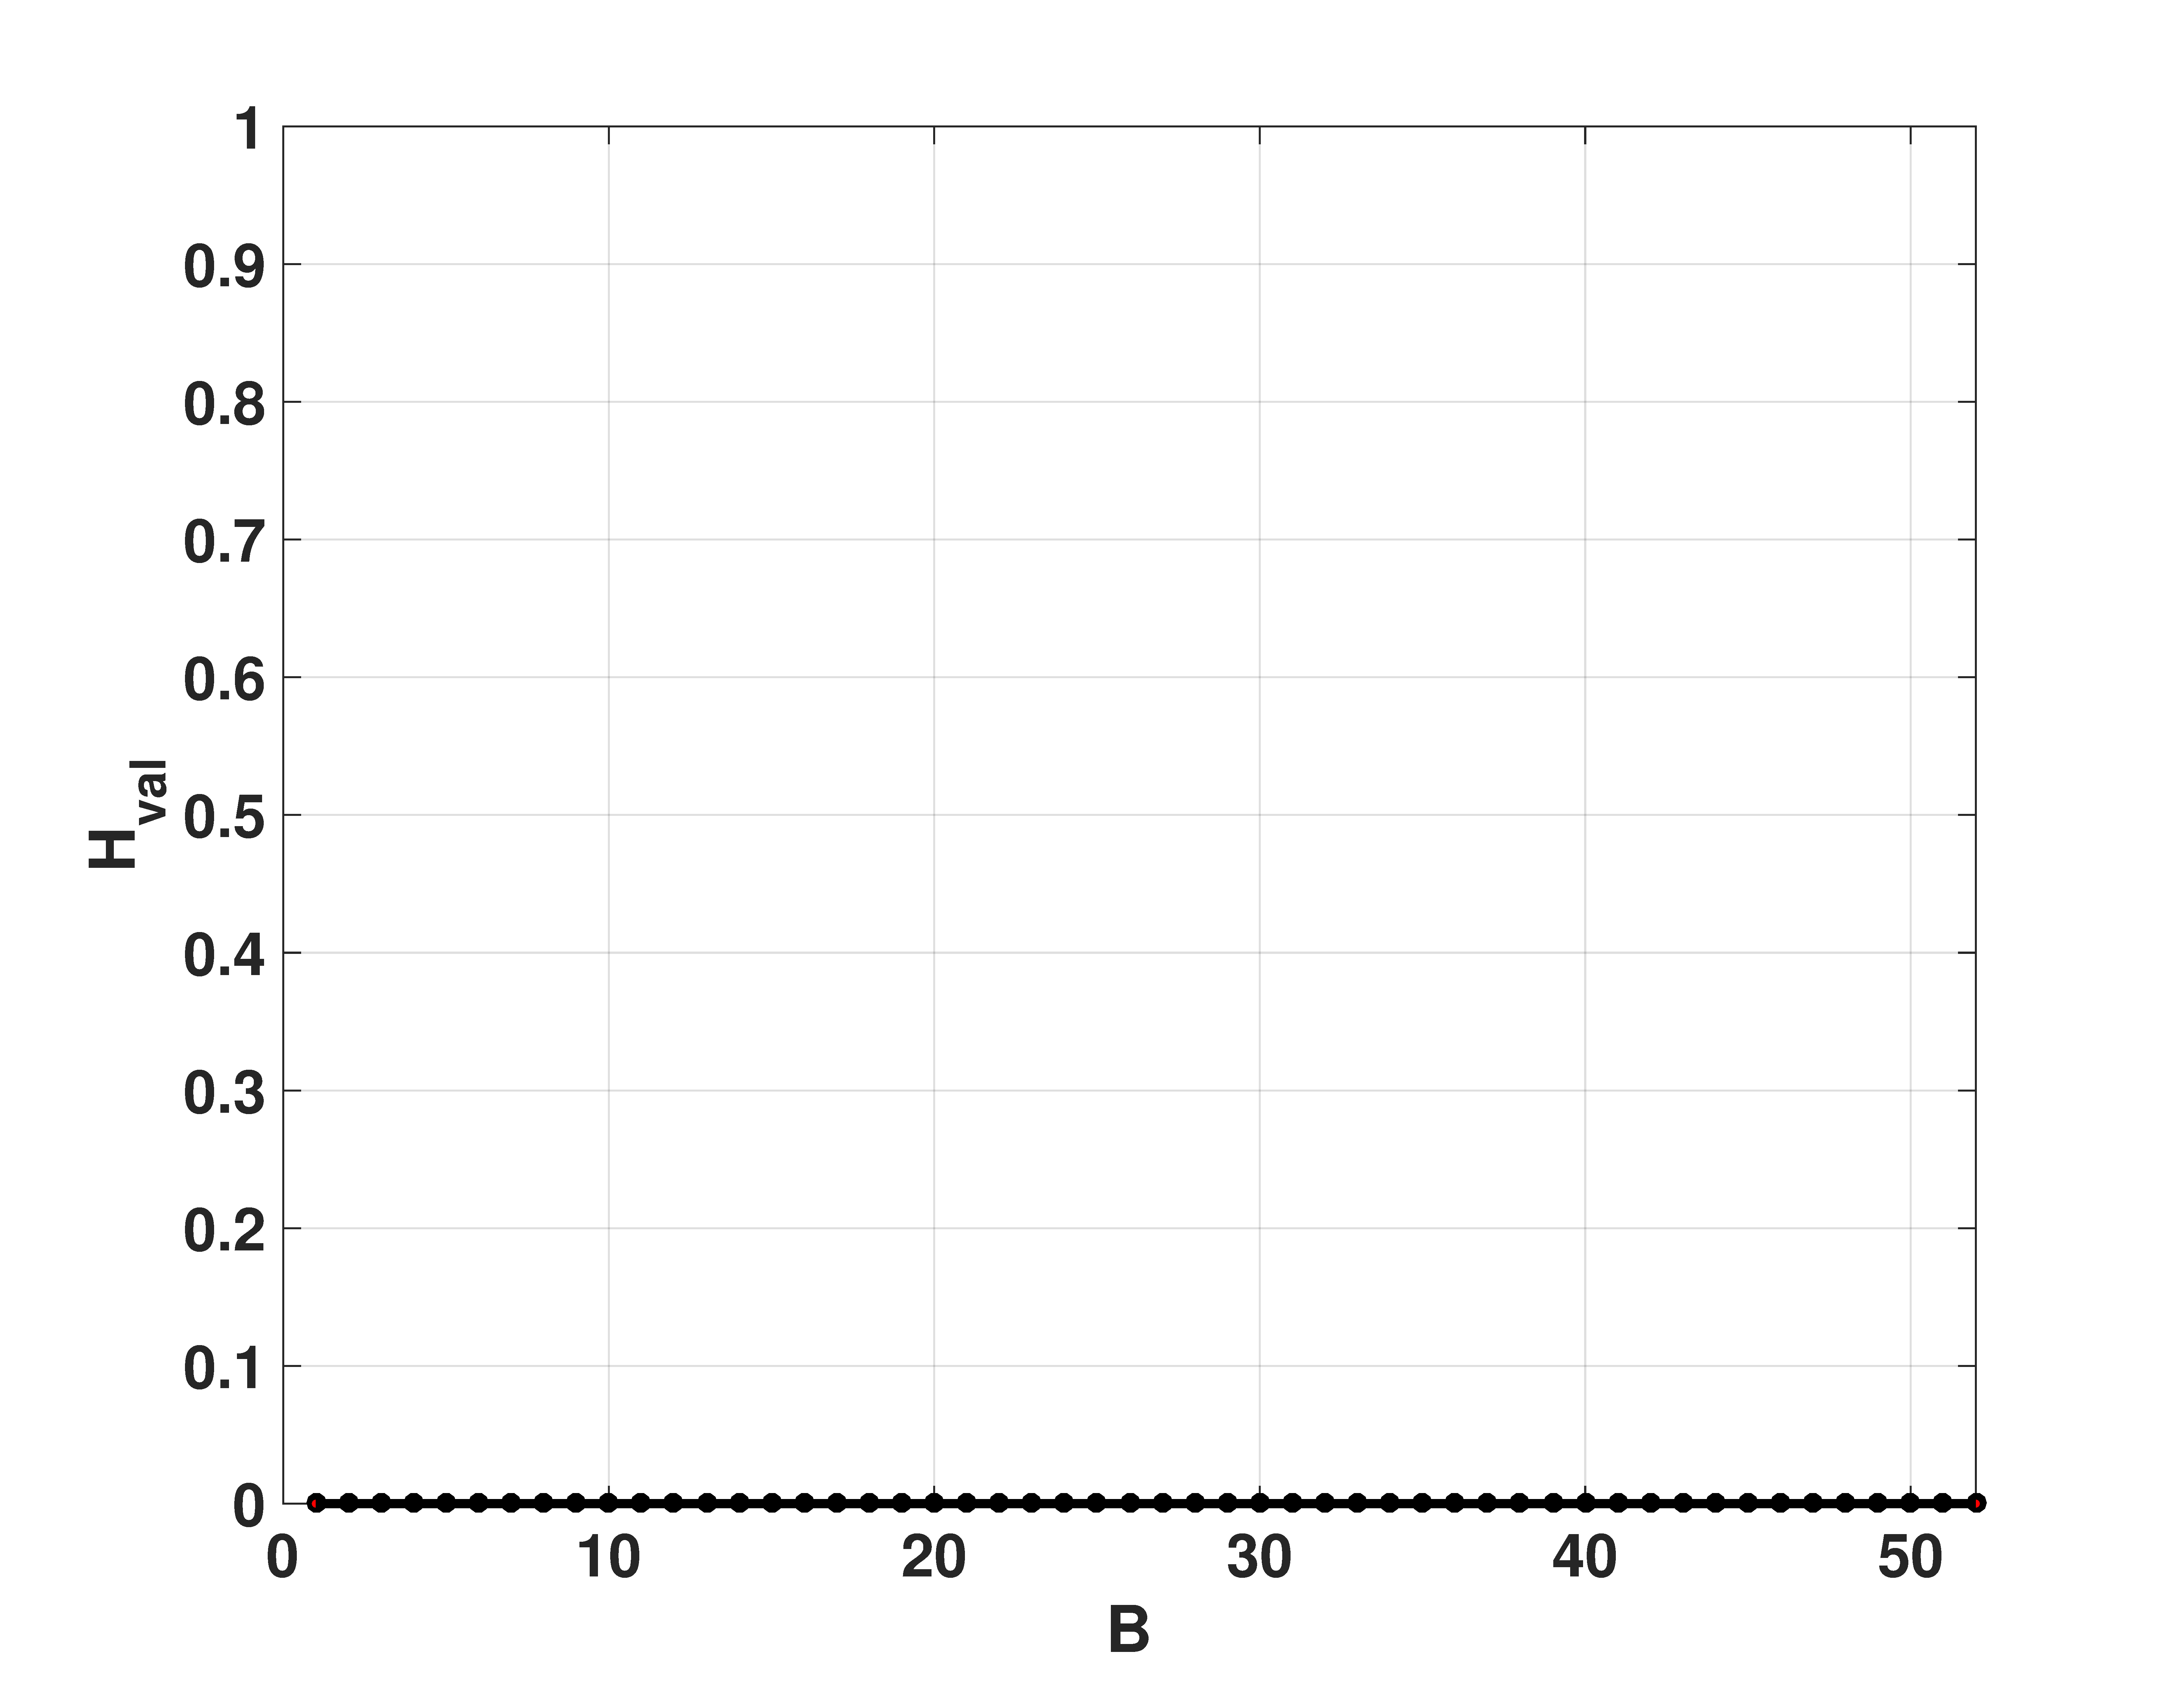
\includegraphics[width=\textwidth]{Hval_Tent}
		\caption{$H_{hist}$ vs. $B$}
		\label{fig:Hval_Tent}
	\end{subfigure}
	\begin{subfigure}[b]{0.49\textwidth}
		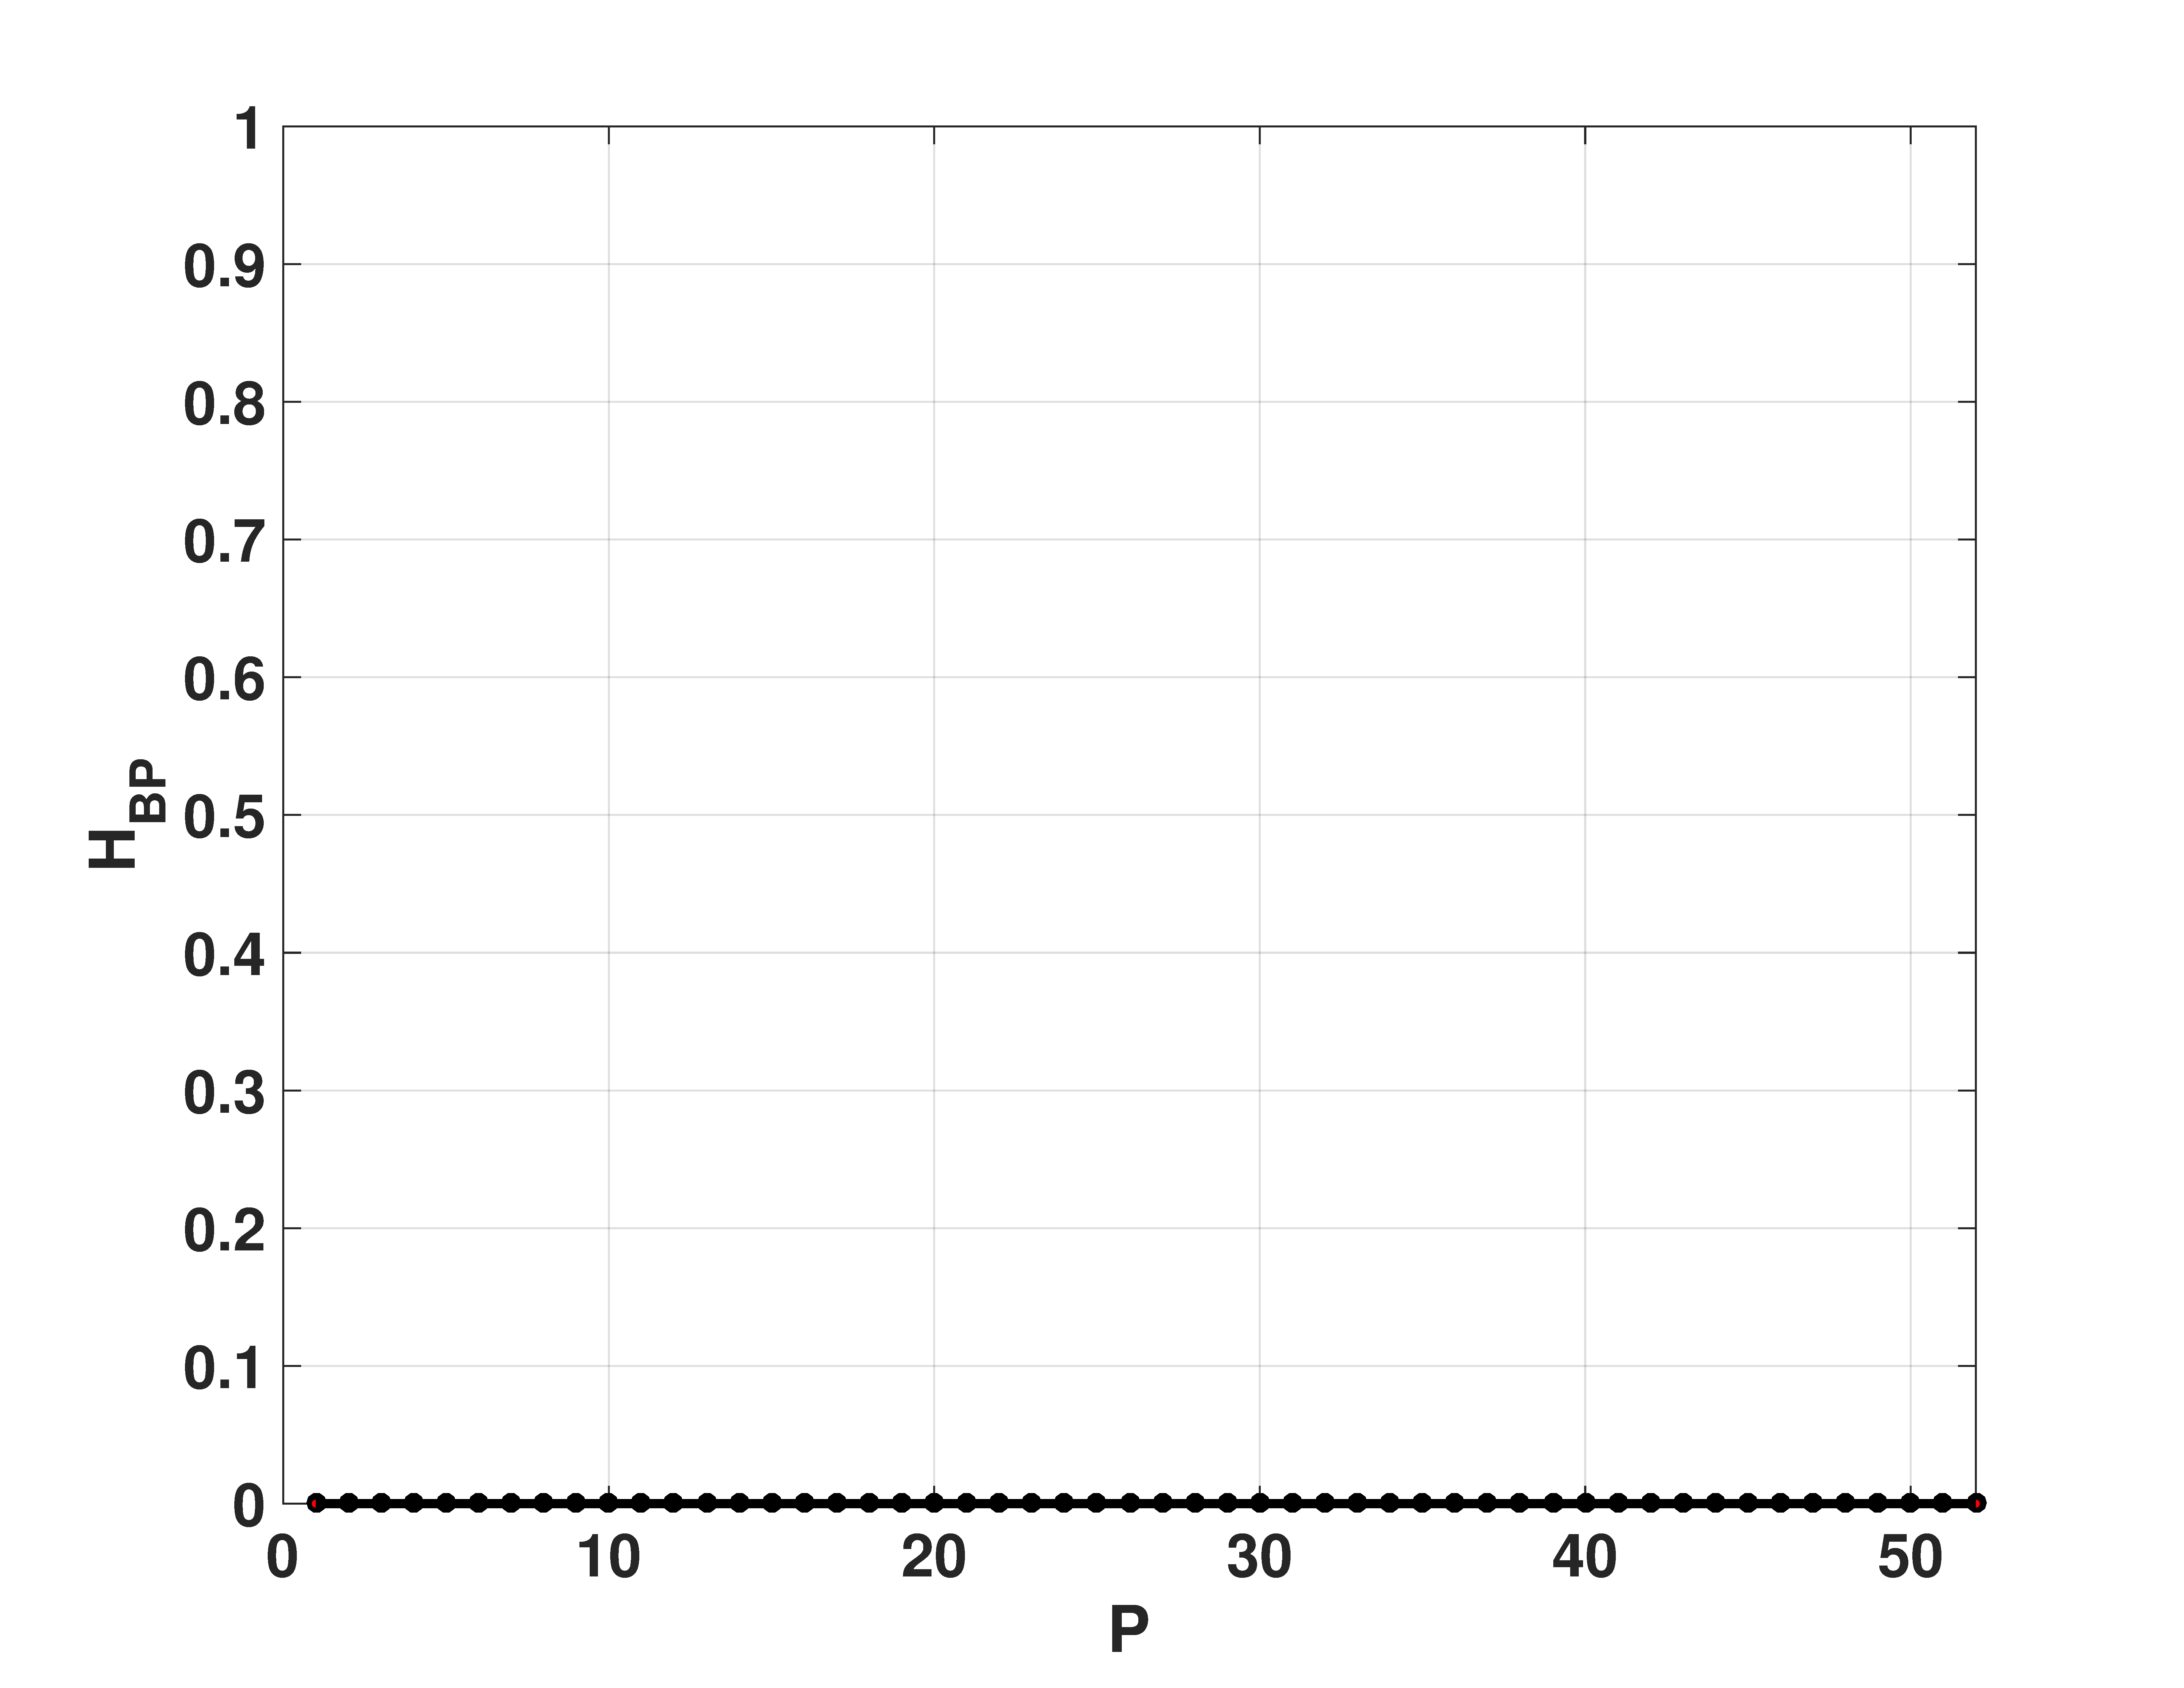
\includegraphics[width=\textwidth]{Hbp_Tent}
		\caption{$H_{BP}$ vs. $B$}
		\label{fig:Hbp_Tent}
	\end{subfigure}
	\begin{subfigure}[b]{0.49\textwidth}
		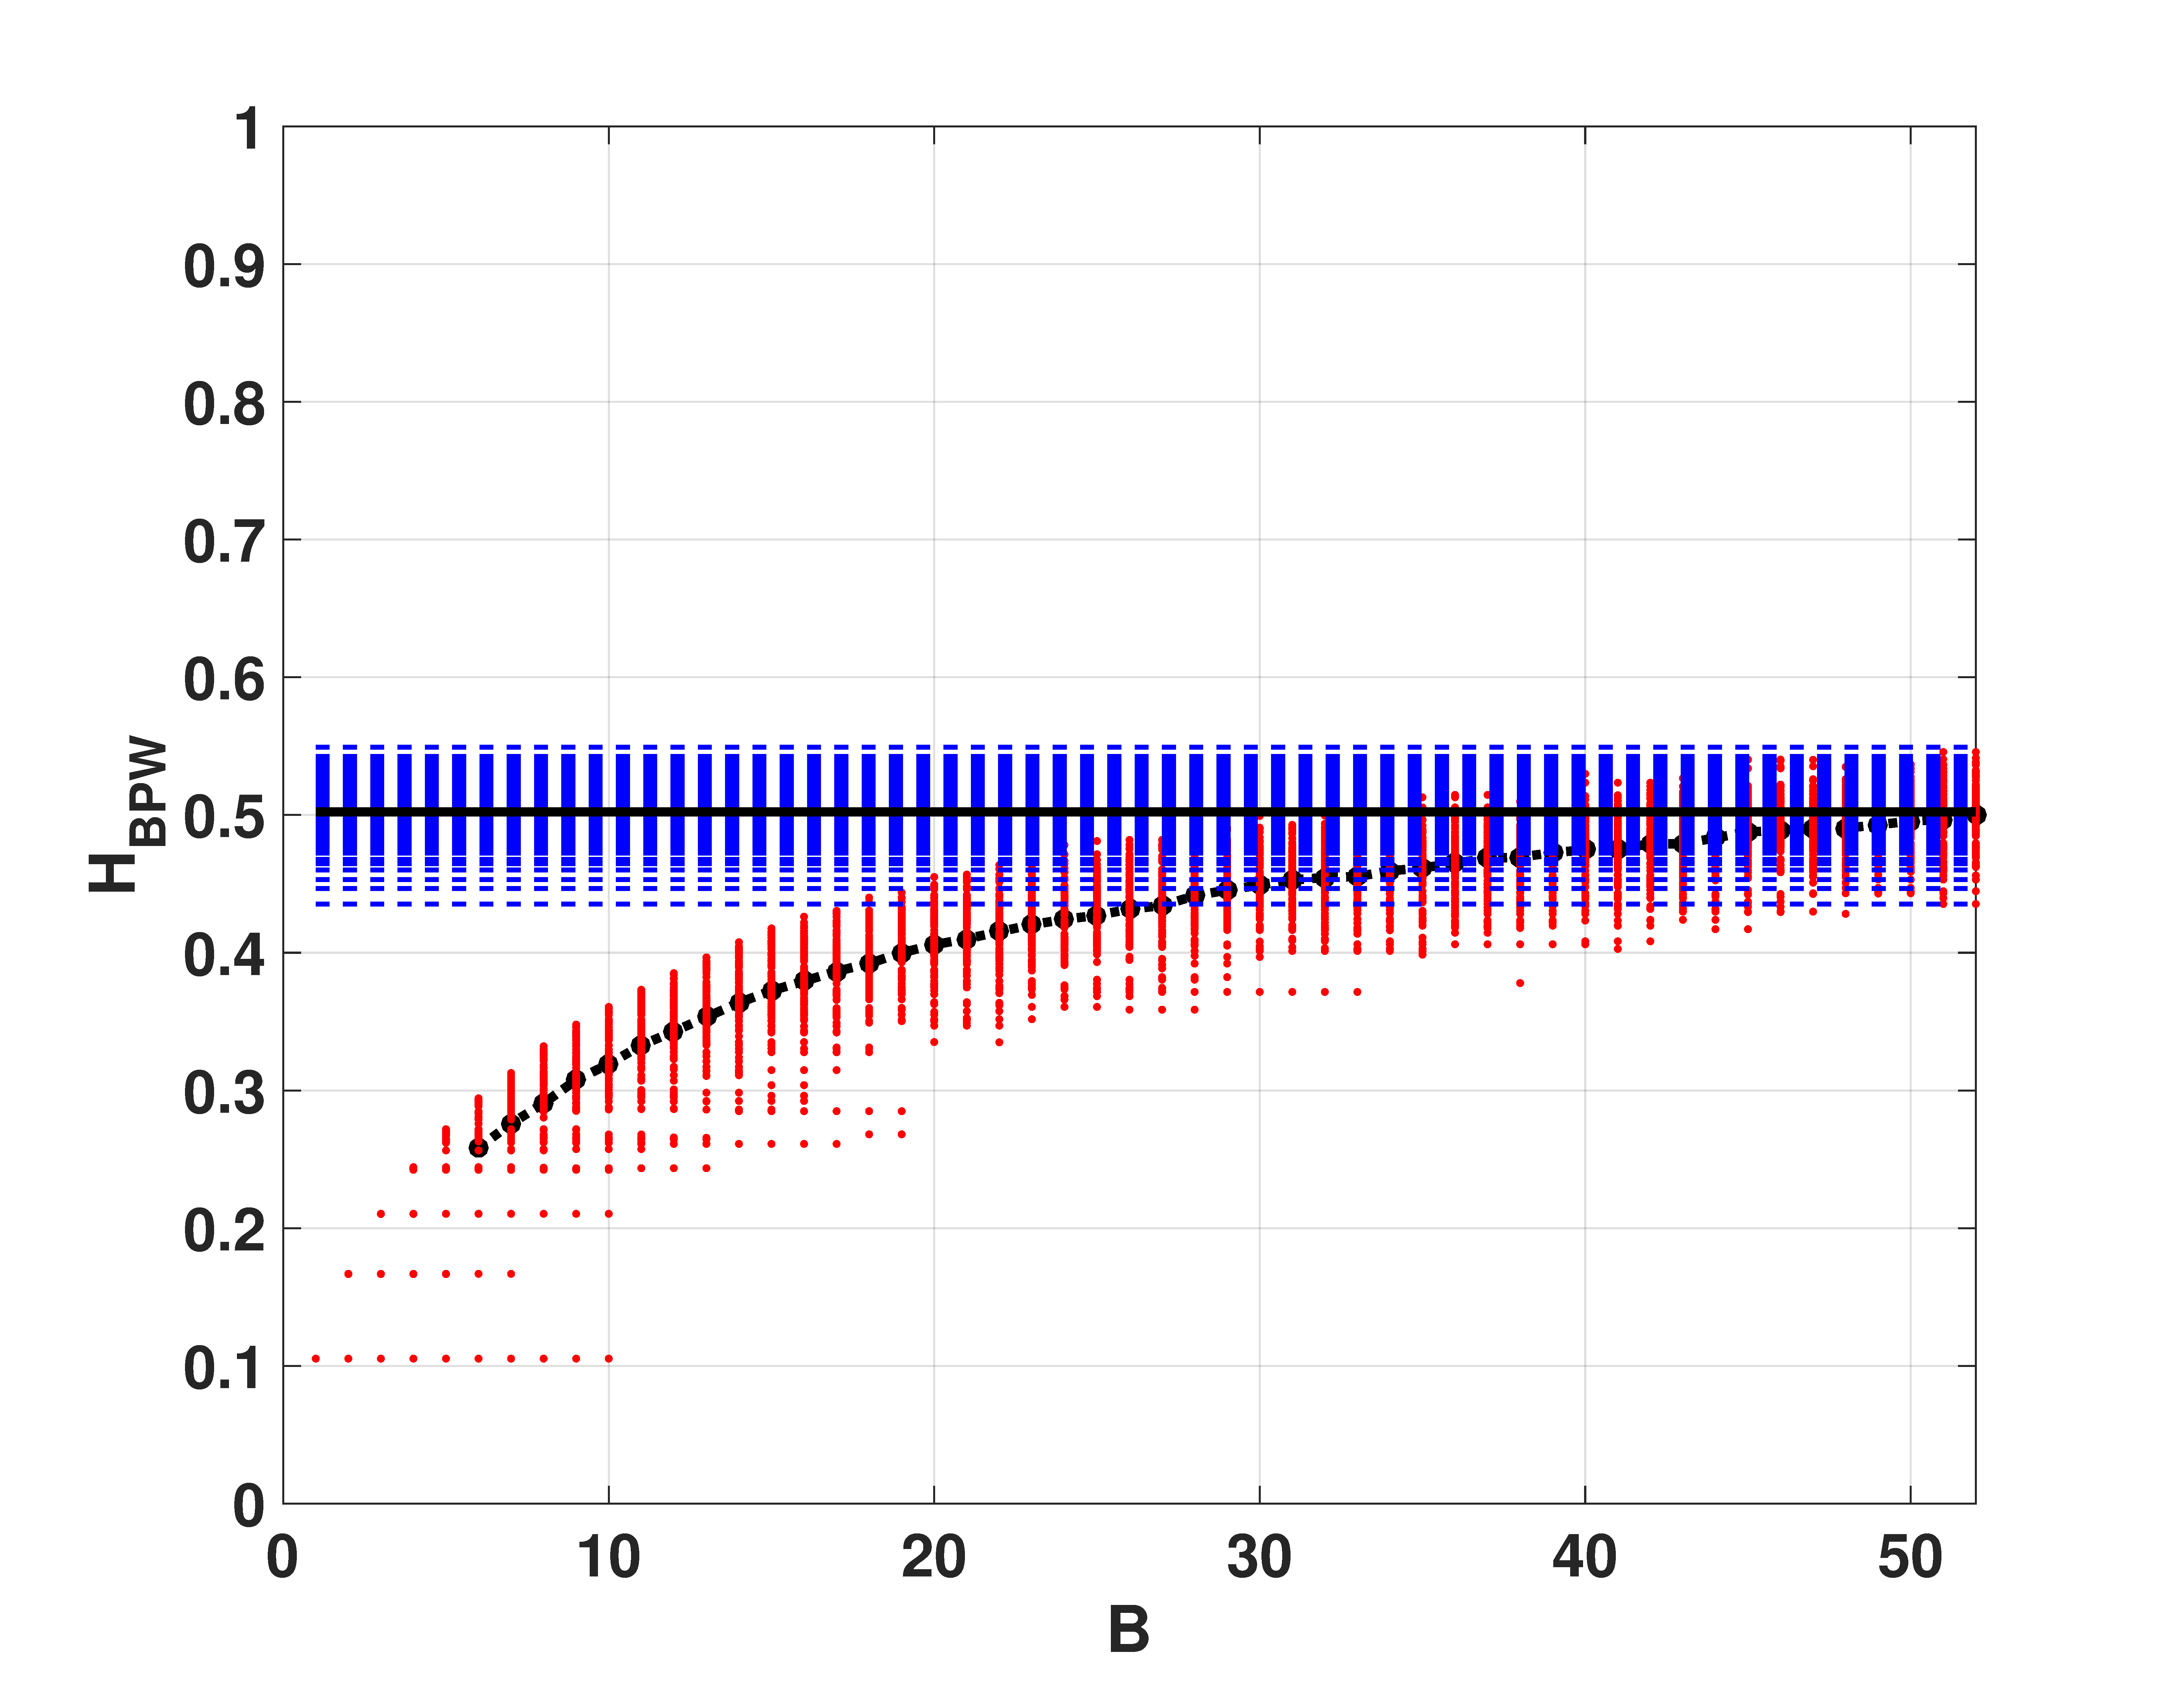
\includegraphics[width=\textwidth]{Hbpw_Tent}
		\caption{$H_{BPW}$ vs. $B$}
		\label{fig:Hbpw_Tent}
	\end{subfigure}
	\begin{subfigure}[b]{0.49\textwidth}
		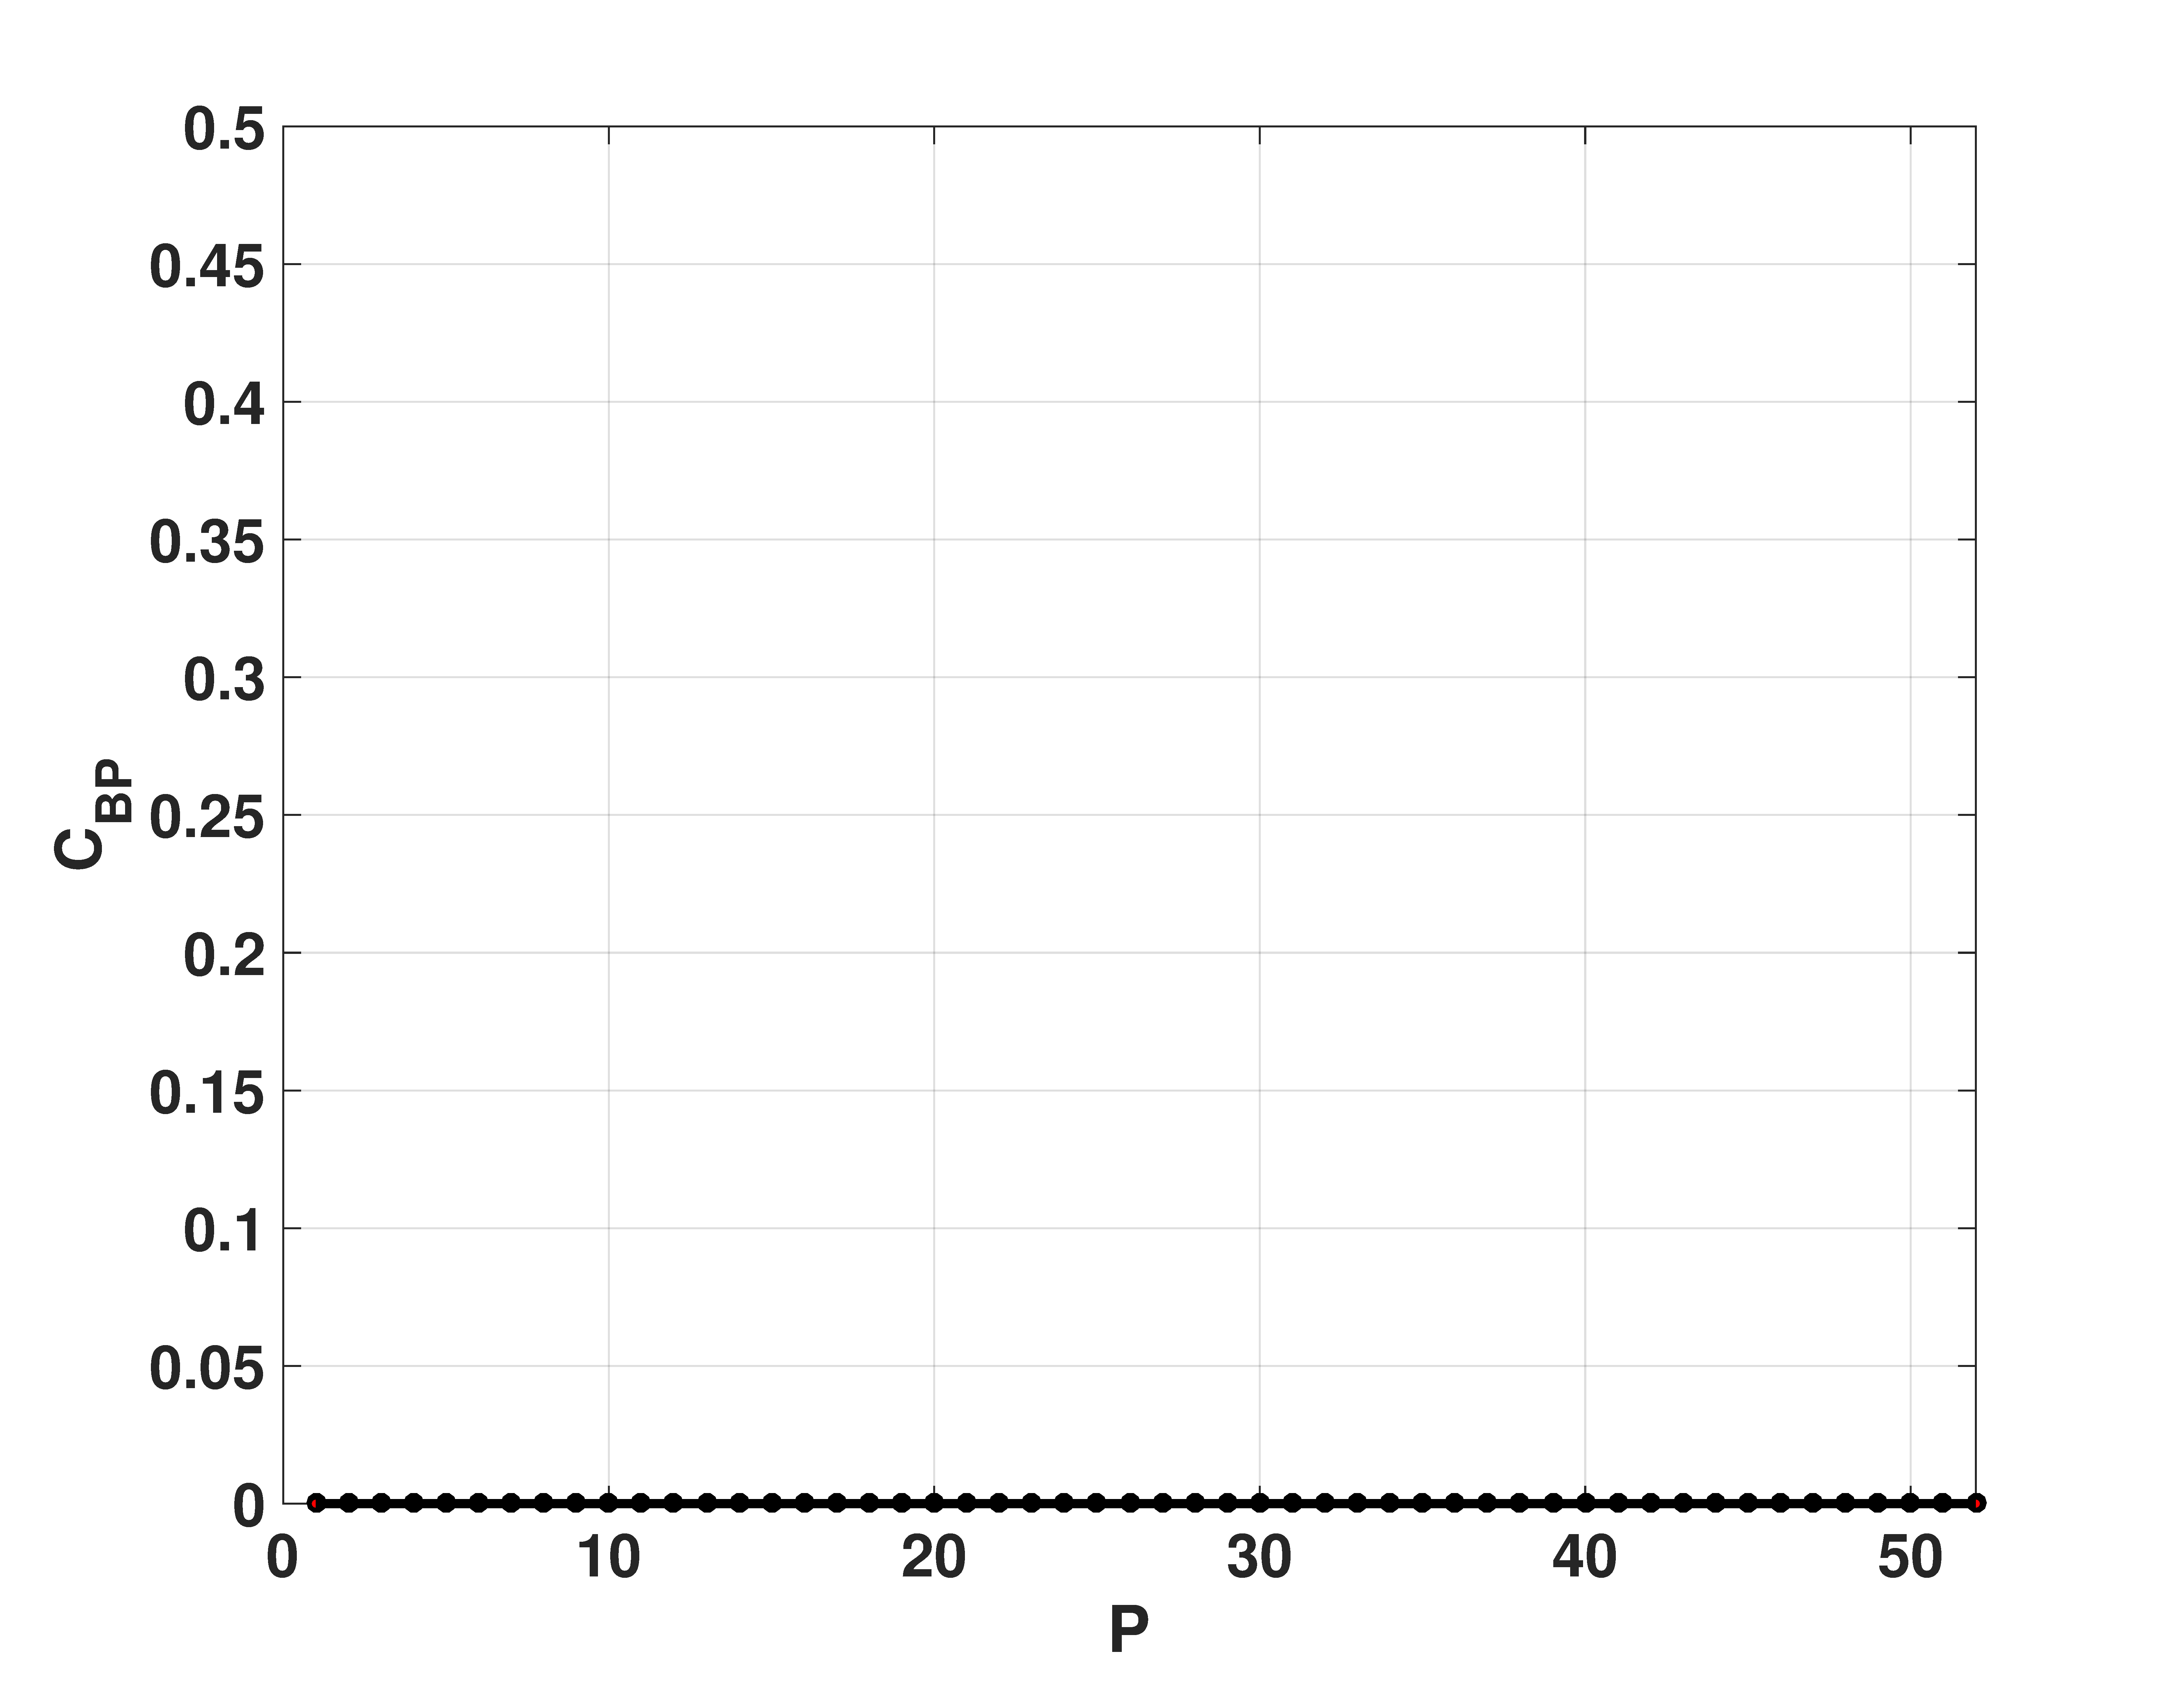
\includegraphics[width=\textwidth]{Cbp_Tent}
		\caption{$C_{BP}$ vs. $B$}
		\label{fig:Cbp_Tent}
	\end{subfigure}
	\begin{subfigure}[b]{0.49\textwidth}
		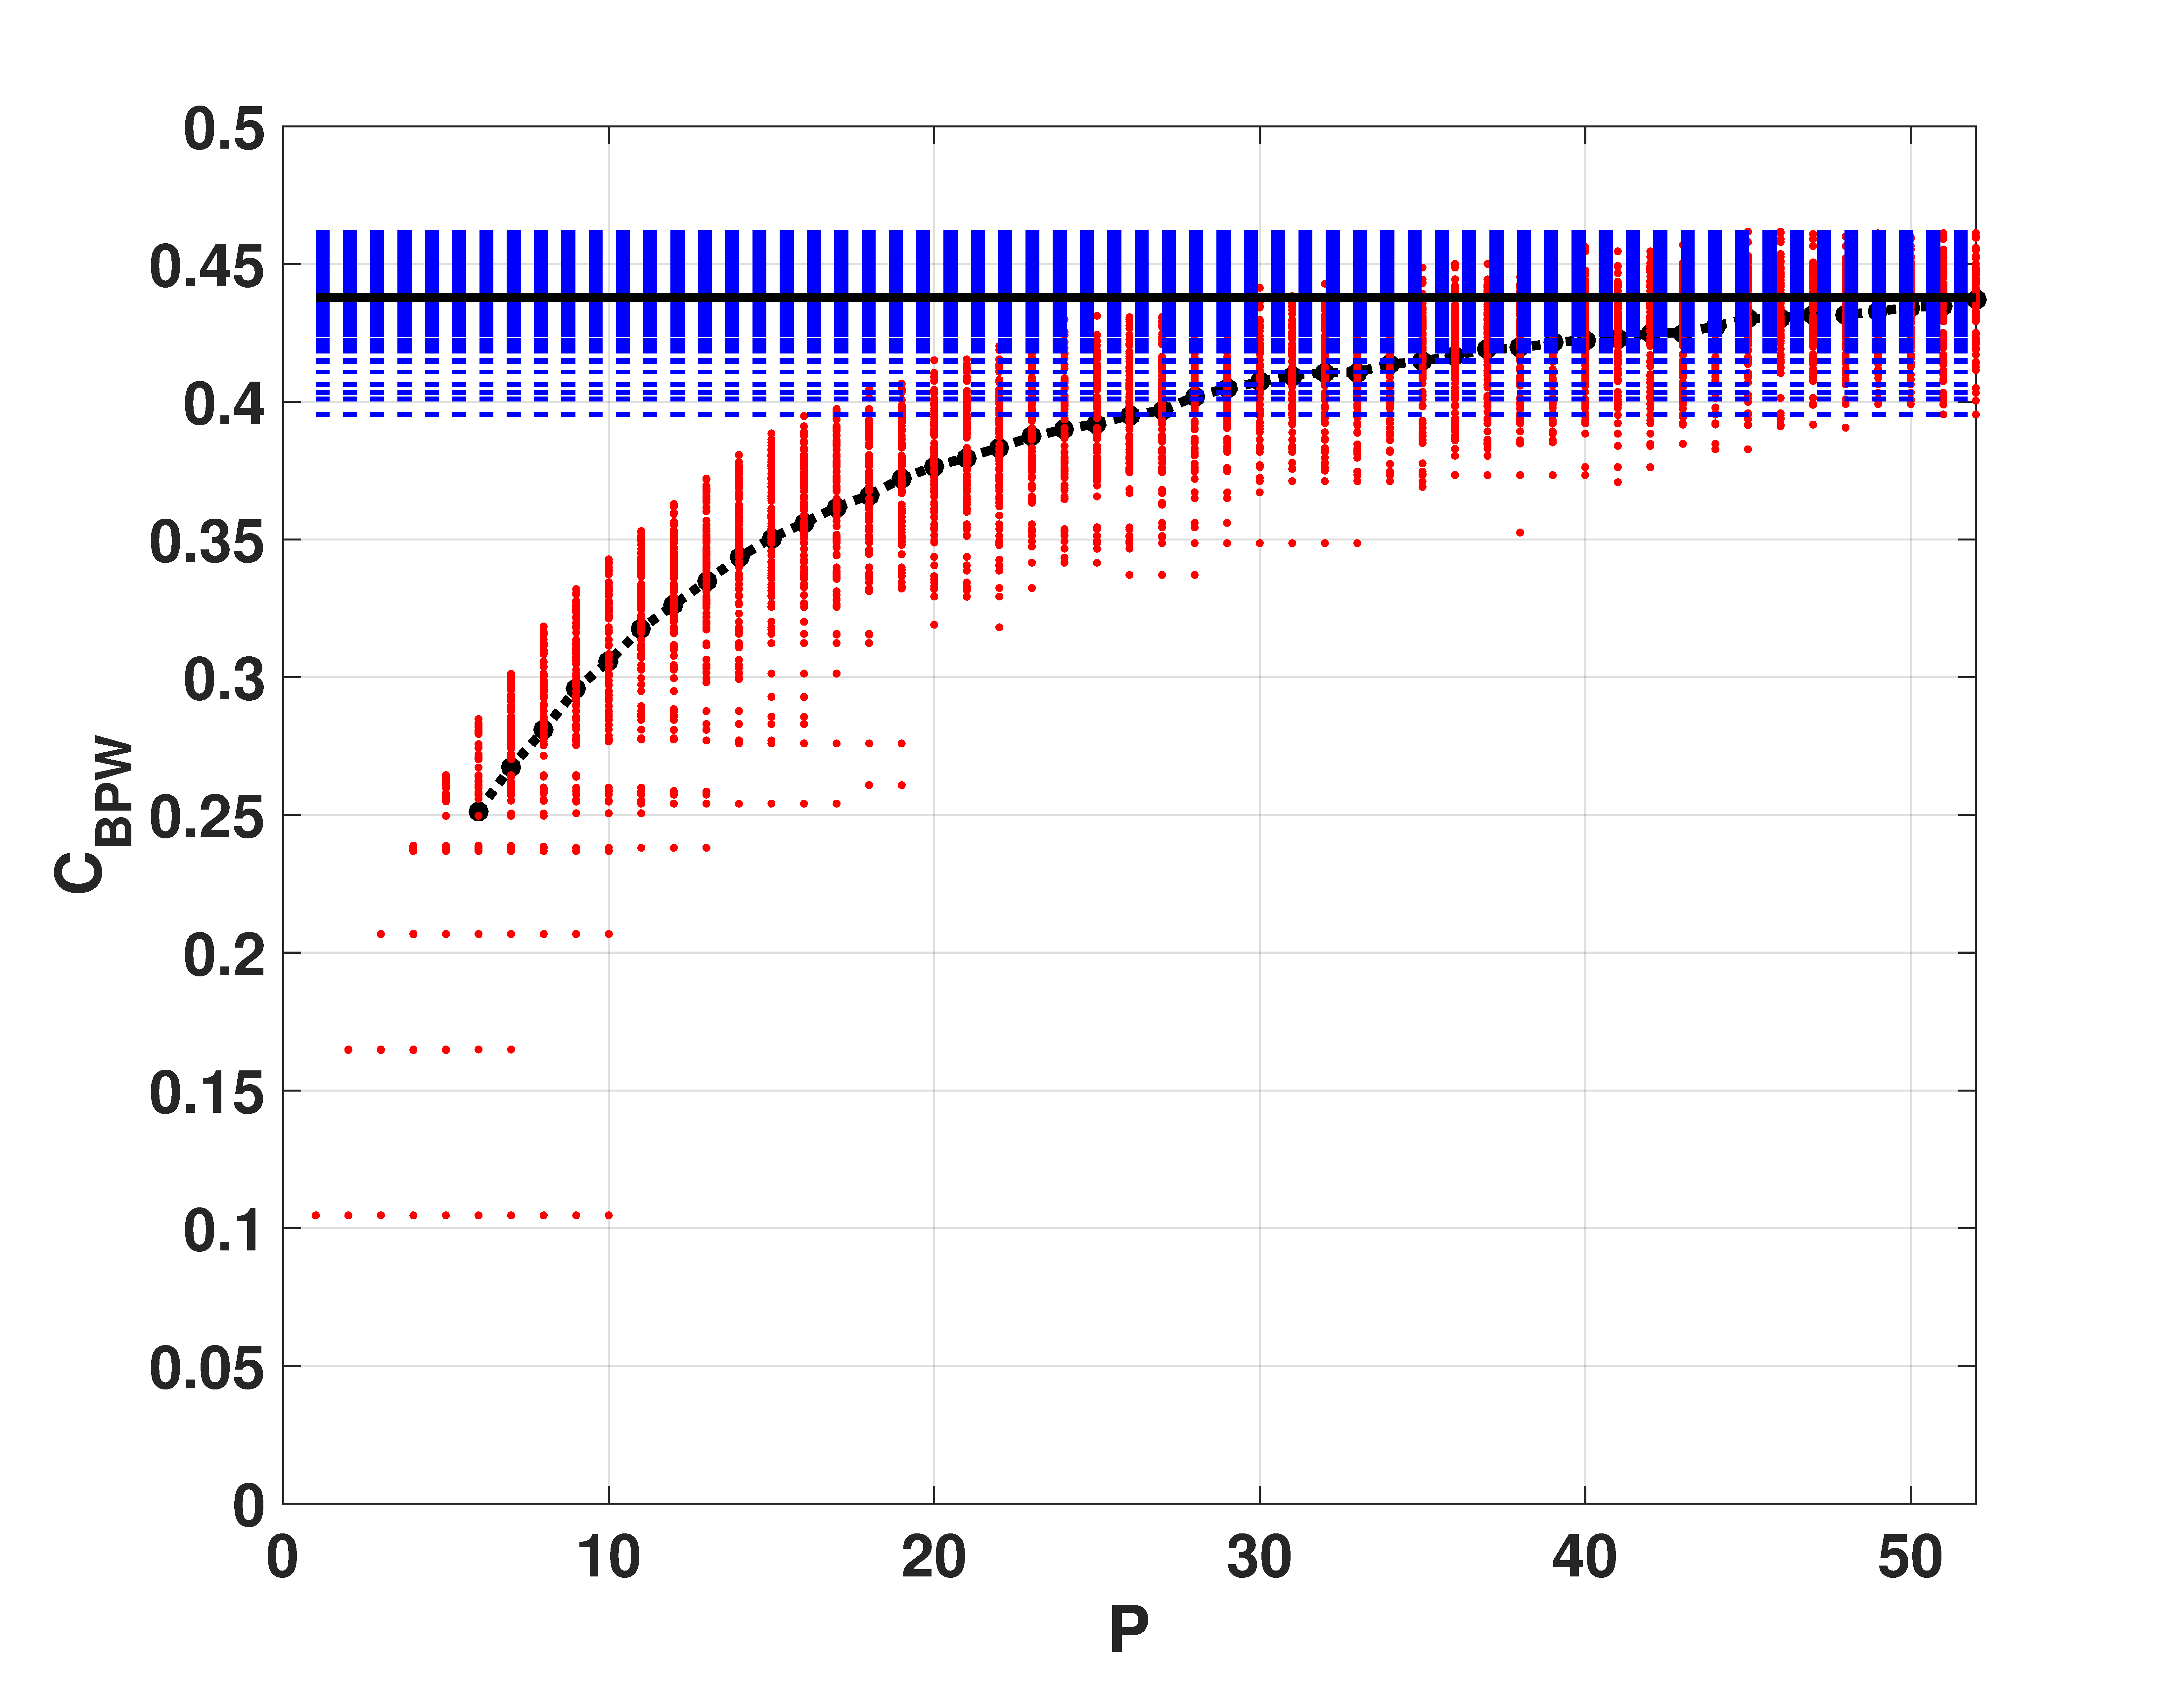
\includegraphics[width=\textwidth]{Cbpw_Tent}
		\caption{$C_{BPW}$ vs. $B$}
		\label{fig:Cbpw_Tent}
	\end{subfigure}
	\begin{subfigure}[b]{0.49\textwidth}
		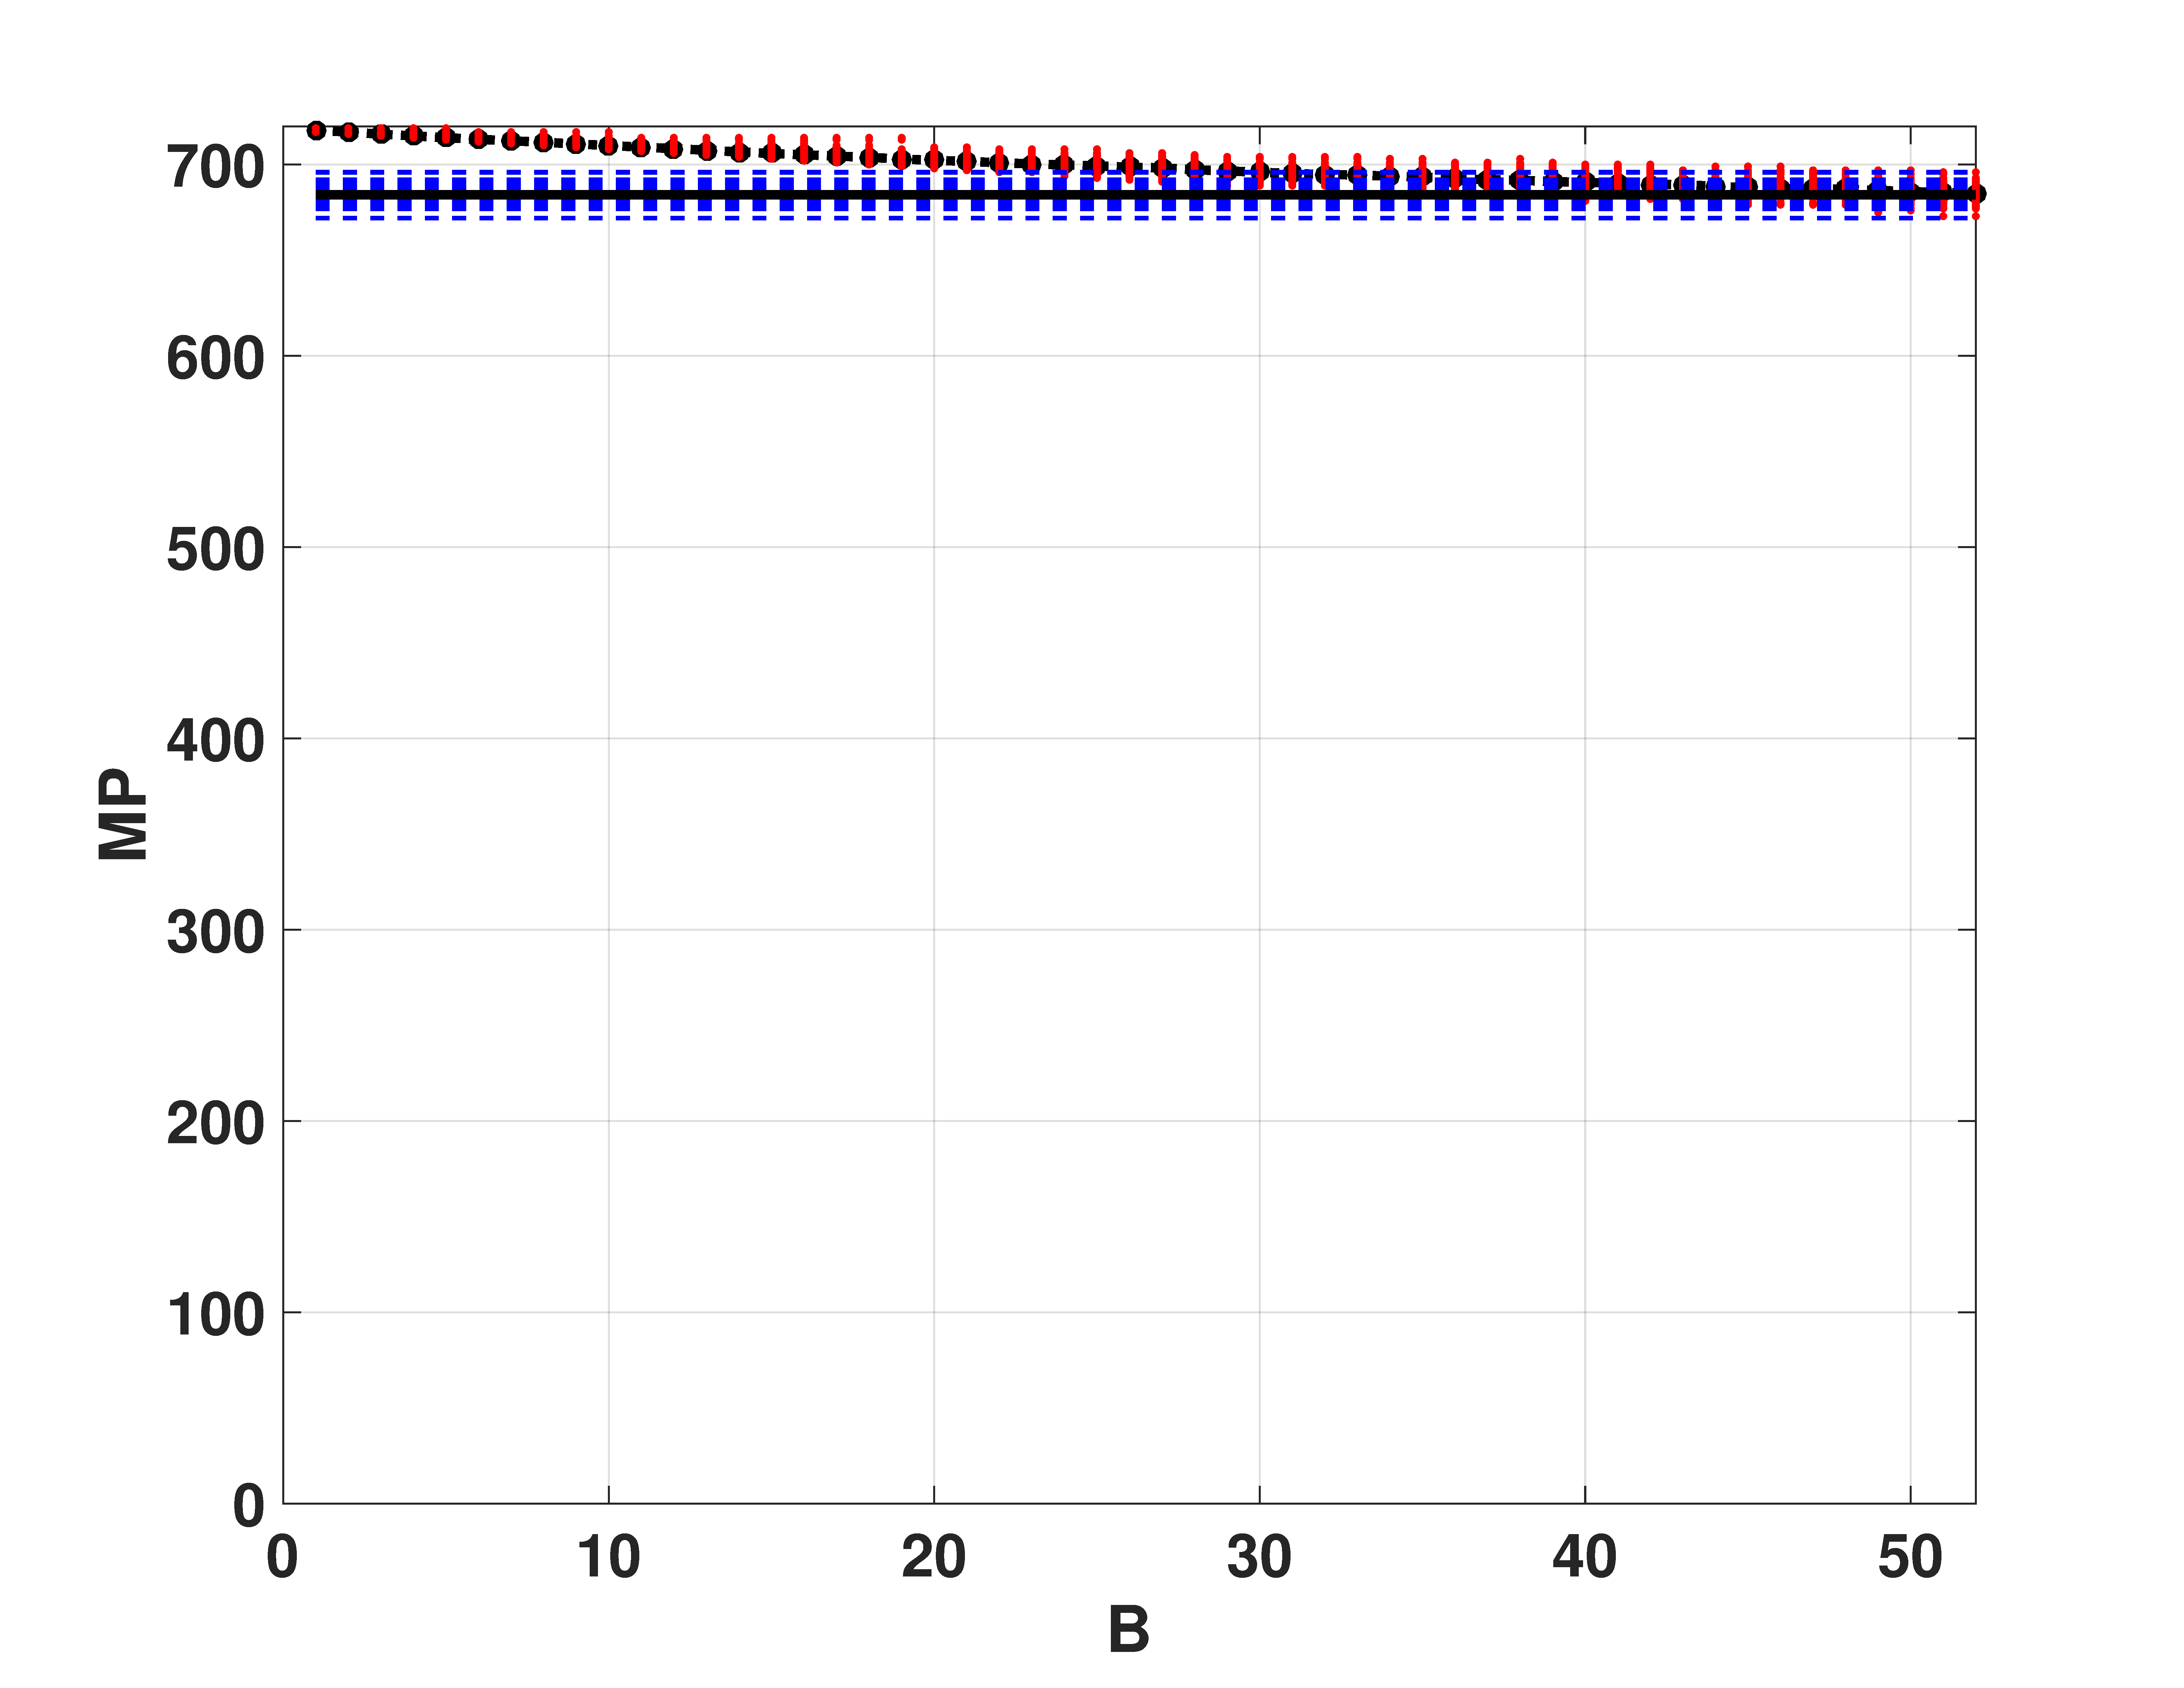
\includegraphics[width=\textwidth]{MP_Tent}
		\caption{MP vs. $B$}
		\label{fig:MP_Tent}
	\end{subfigure}
	\caption{Statistical properties of TENT map}
	\label{fig:TENT_QuantiB}
\end{figure}

Summarizing, in spite of using a high number of bits (with any 2-based numerical representation) to represent the digitalized TENT map it always loses the chaotic behaviour.
 

\subsection{Quantifiers of combined Maps}\label{subsec:SecSwitch}
Here we report our results for the three combinations of the simple maps, SWITCH, EVEN and ODD.

\subsubsection{Sequential switching between Tent and Logistic maps (SWITCH)} \label{sssec:switch}

SWITCH map is expressed as:

\begin{equation}
\begin{cases}
	x_{n+1}=
	\begin{cases}
		2x_n, & \mbox{if } 0\leq x_n\leq 1/2 \\
		2(1-x_n ), & \mbox{if } 1/2<x_n\leq 1
	\end{cases} \\
	x_{n+2}=4x_{n+1}(1-x_{n+1})
\end{cases}\label{eq:SWITCH}
\end{equation}
with $x_n\in\mathcal{R}$ and $n$ an even number.

Results with sequential switching are shown in Figs. \ref{fig:SWITCH_QuantiB} (a) to (f).
The entropy value calculated in floating point is $H_{val}=0.9722$, this value is slightly higher than the one obtained for the LOG map. 
For fixed point arithmetic this value is reached in $B=24$, but it stabilizes from $B=28$.
Regarding the ordering patterns the number of MP decreases to $586$, this value lower than the one obtained for LOG map.
It means the entropy $H_{BP}$ may increase up to $ln(134)/ln(720)\simeq 0.74$.
$BP$ and $BPW$ quantifiers reach their maximum of $H_{BP}=0.6546$ and $H_{BPW}=0.6313$ at $B=16$, but they stabilize from $B=24$.
Complexities are lower than for LOG, $C_{BP}=0.4580$ and $C_{BPW}=0.4578$, these values are reached for $B \geq 15$ but they are stable from $B \geq 23$.
Compared with LOG, statistical properties are better with less amount of bits, for $B \geq 24$ this map reaches optimal characteristics in the sense of random source.

\textcolor{red}{ESTO NO SE SI VA A IR EN LONG DOUBLE}
We can see some points with anomalies from $B \geq 49$ due to the same problem of LOG map, an multiplication needs double of precision to be done.
Furthermore, we encountred one initial condition in fixed point with an anomalous behaviour.

\begin{figure}
	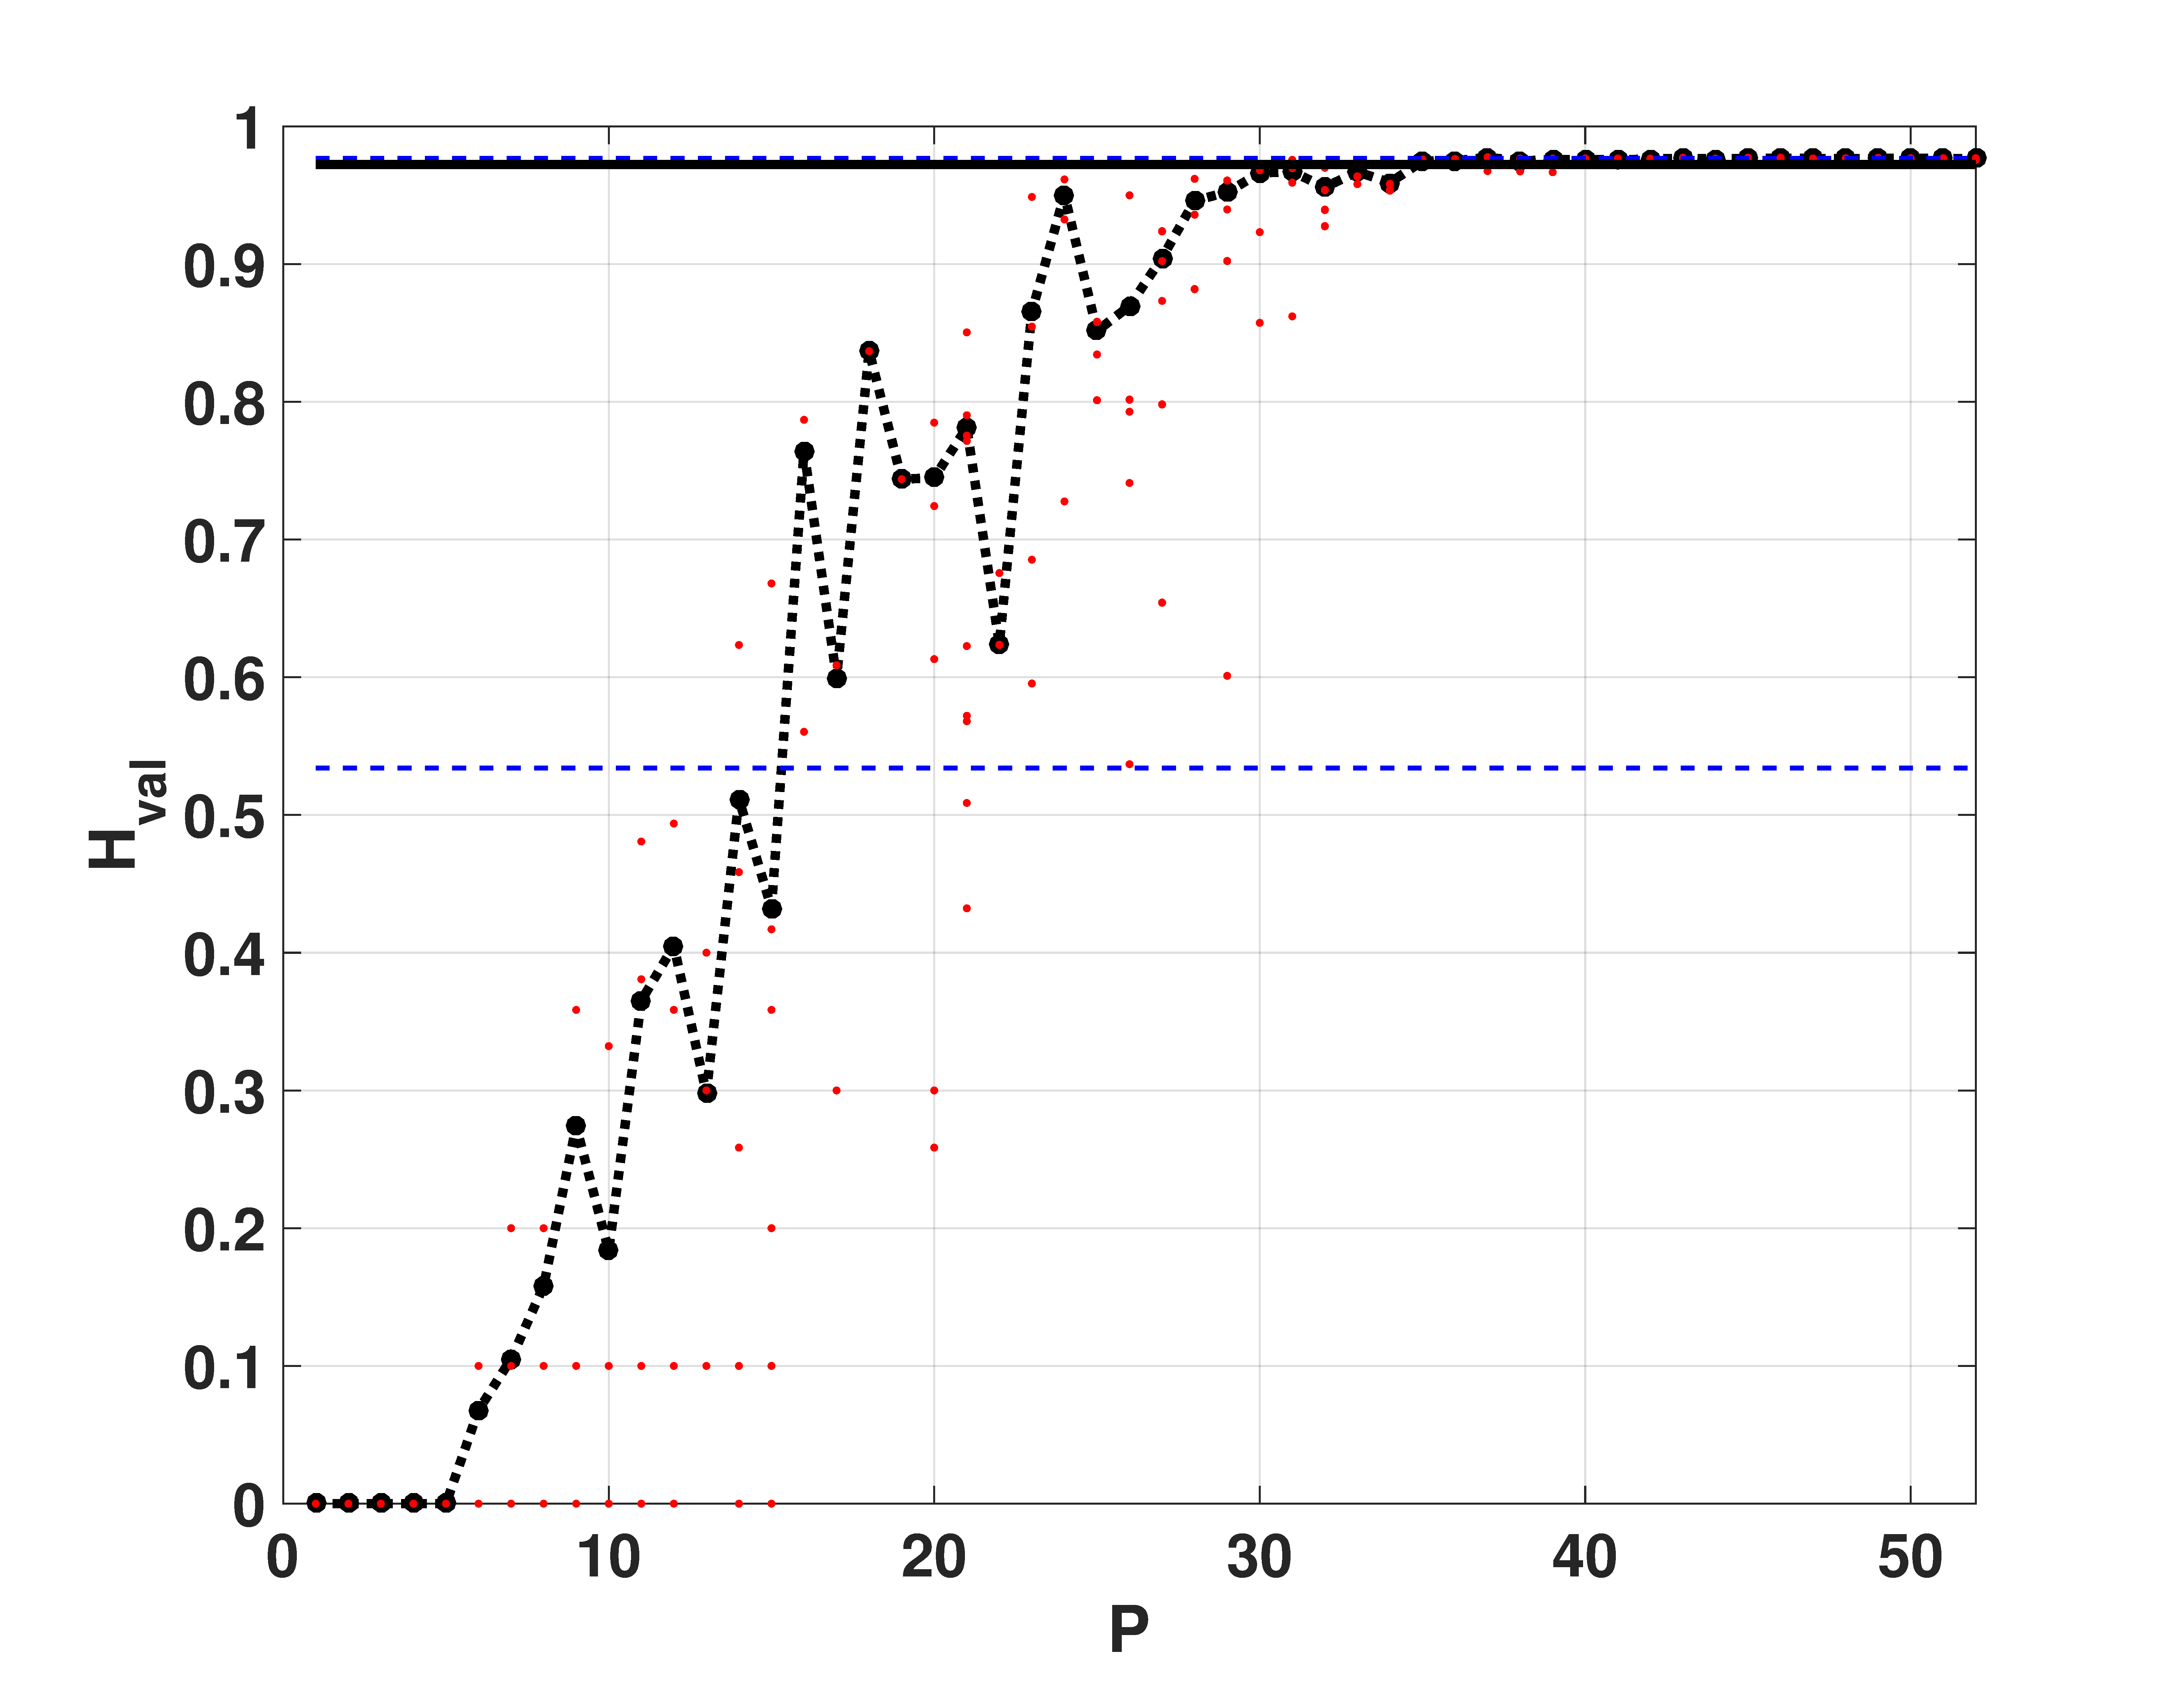
\includegraphics[width=.49\textwidth]{Hval_Switch}
	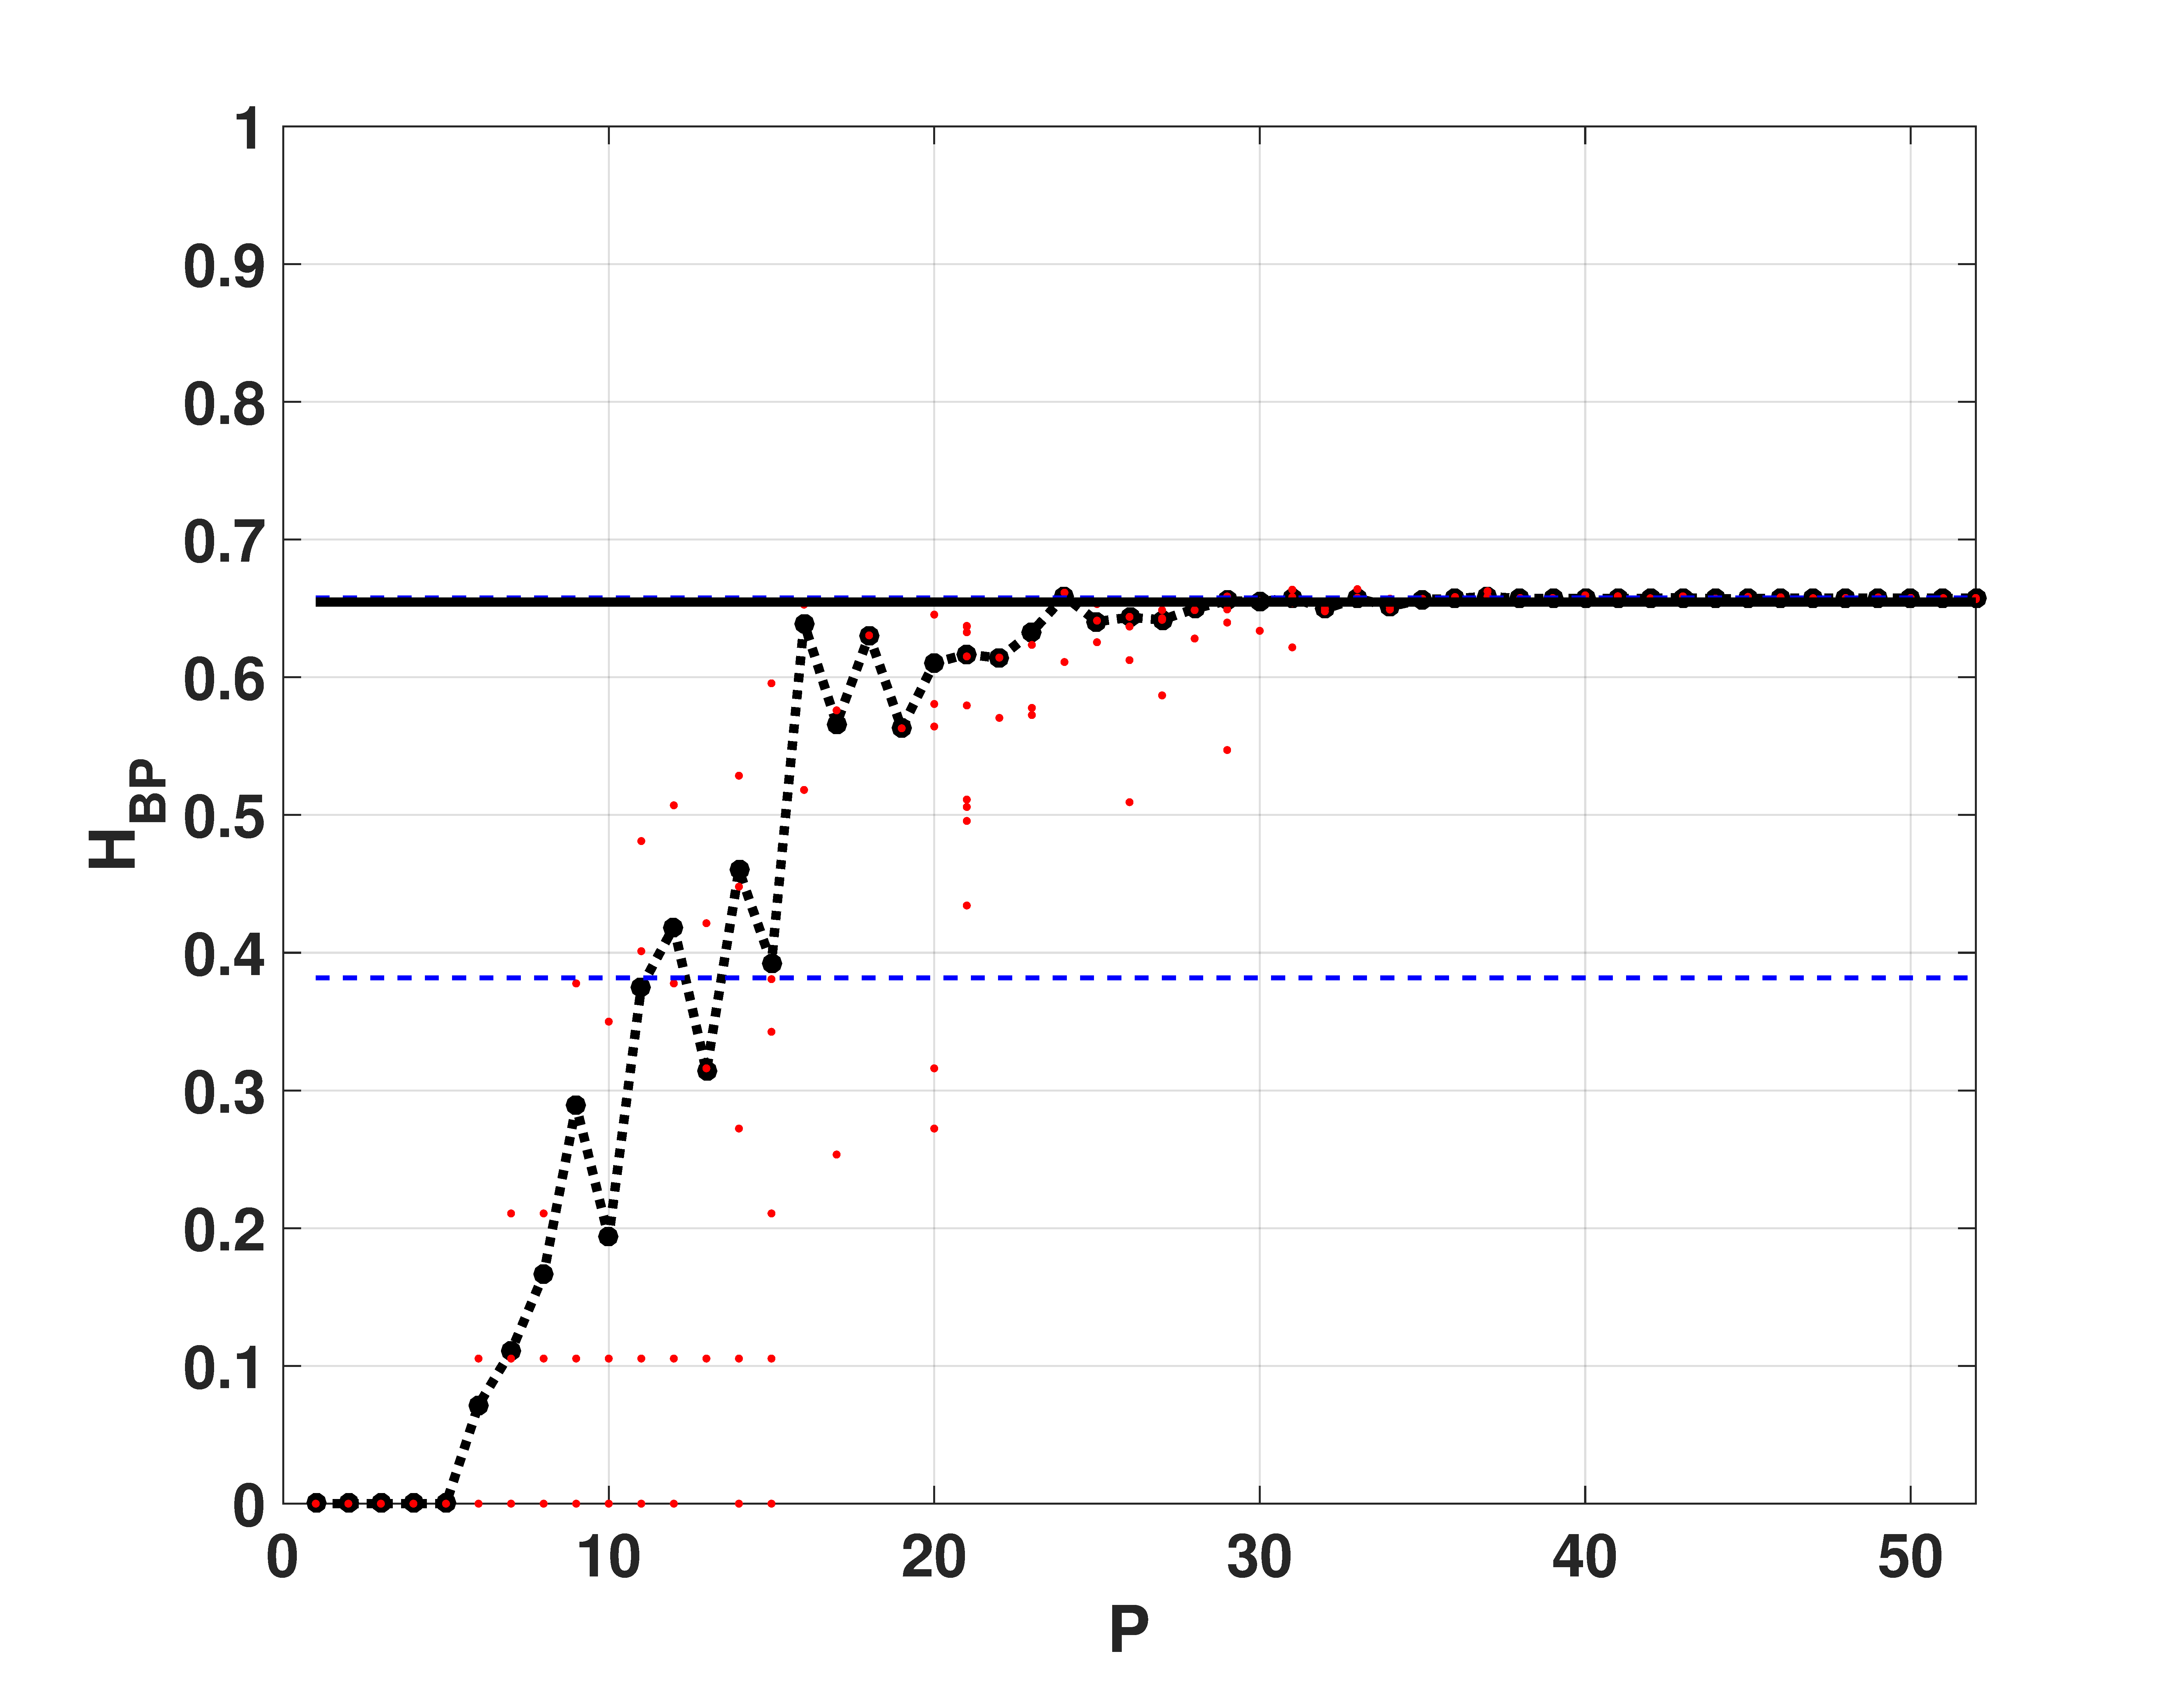
\includegraphics[width=.49\textwidth]{Hbp_Switch}
	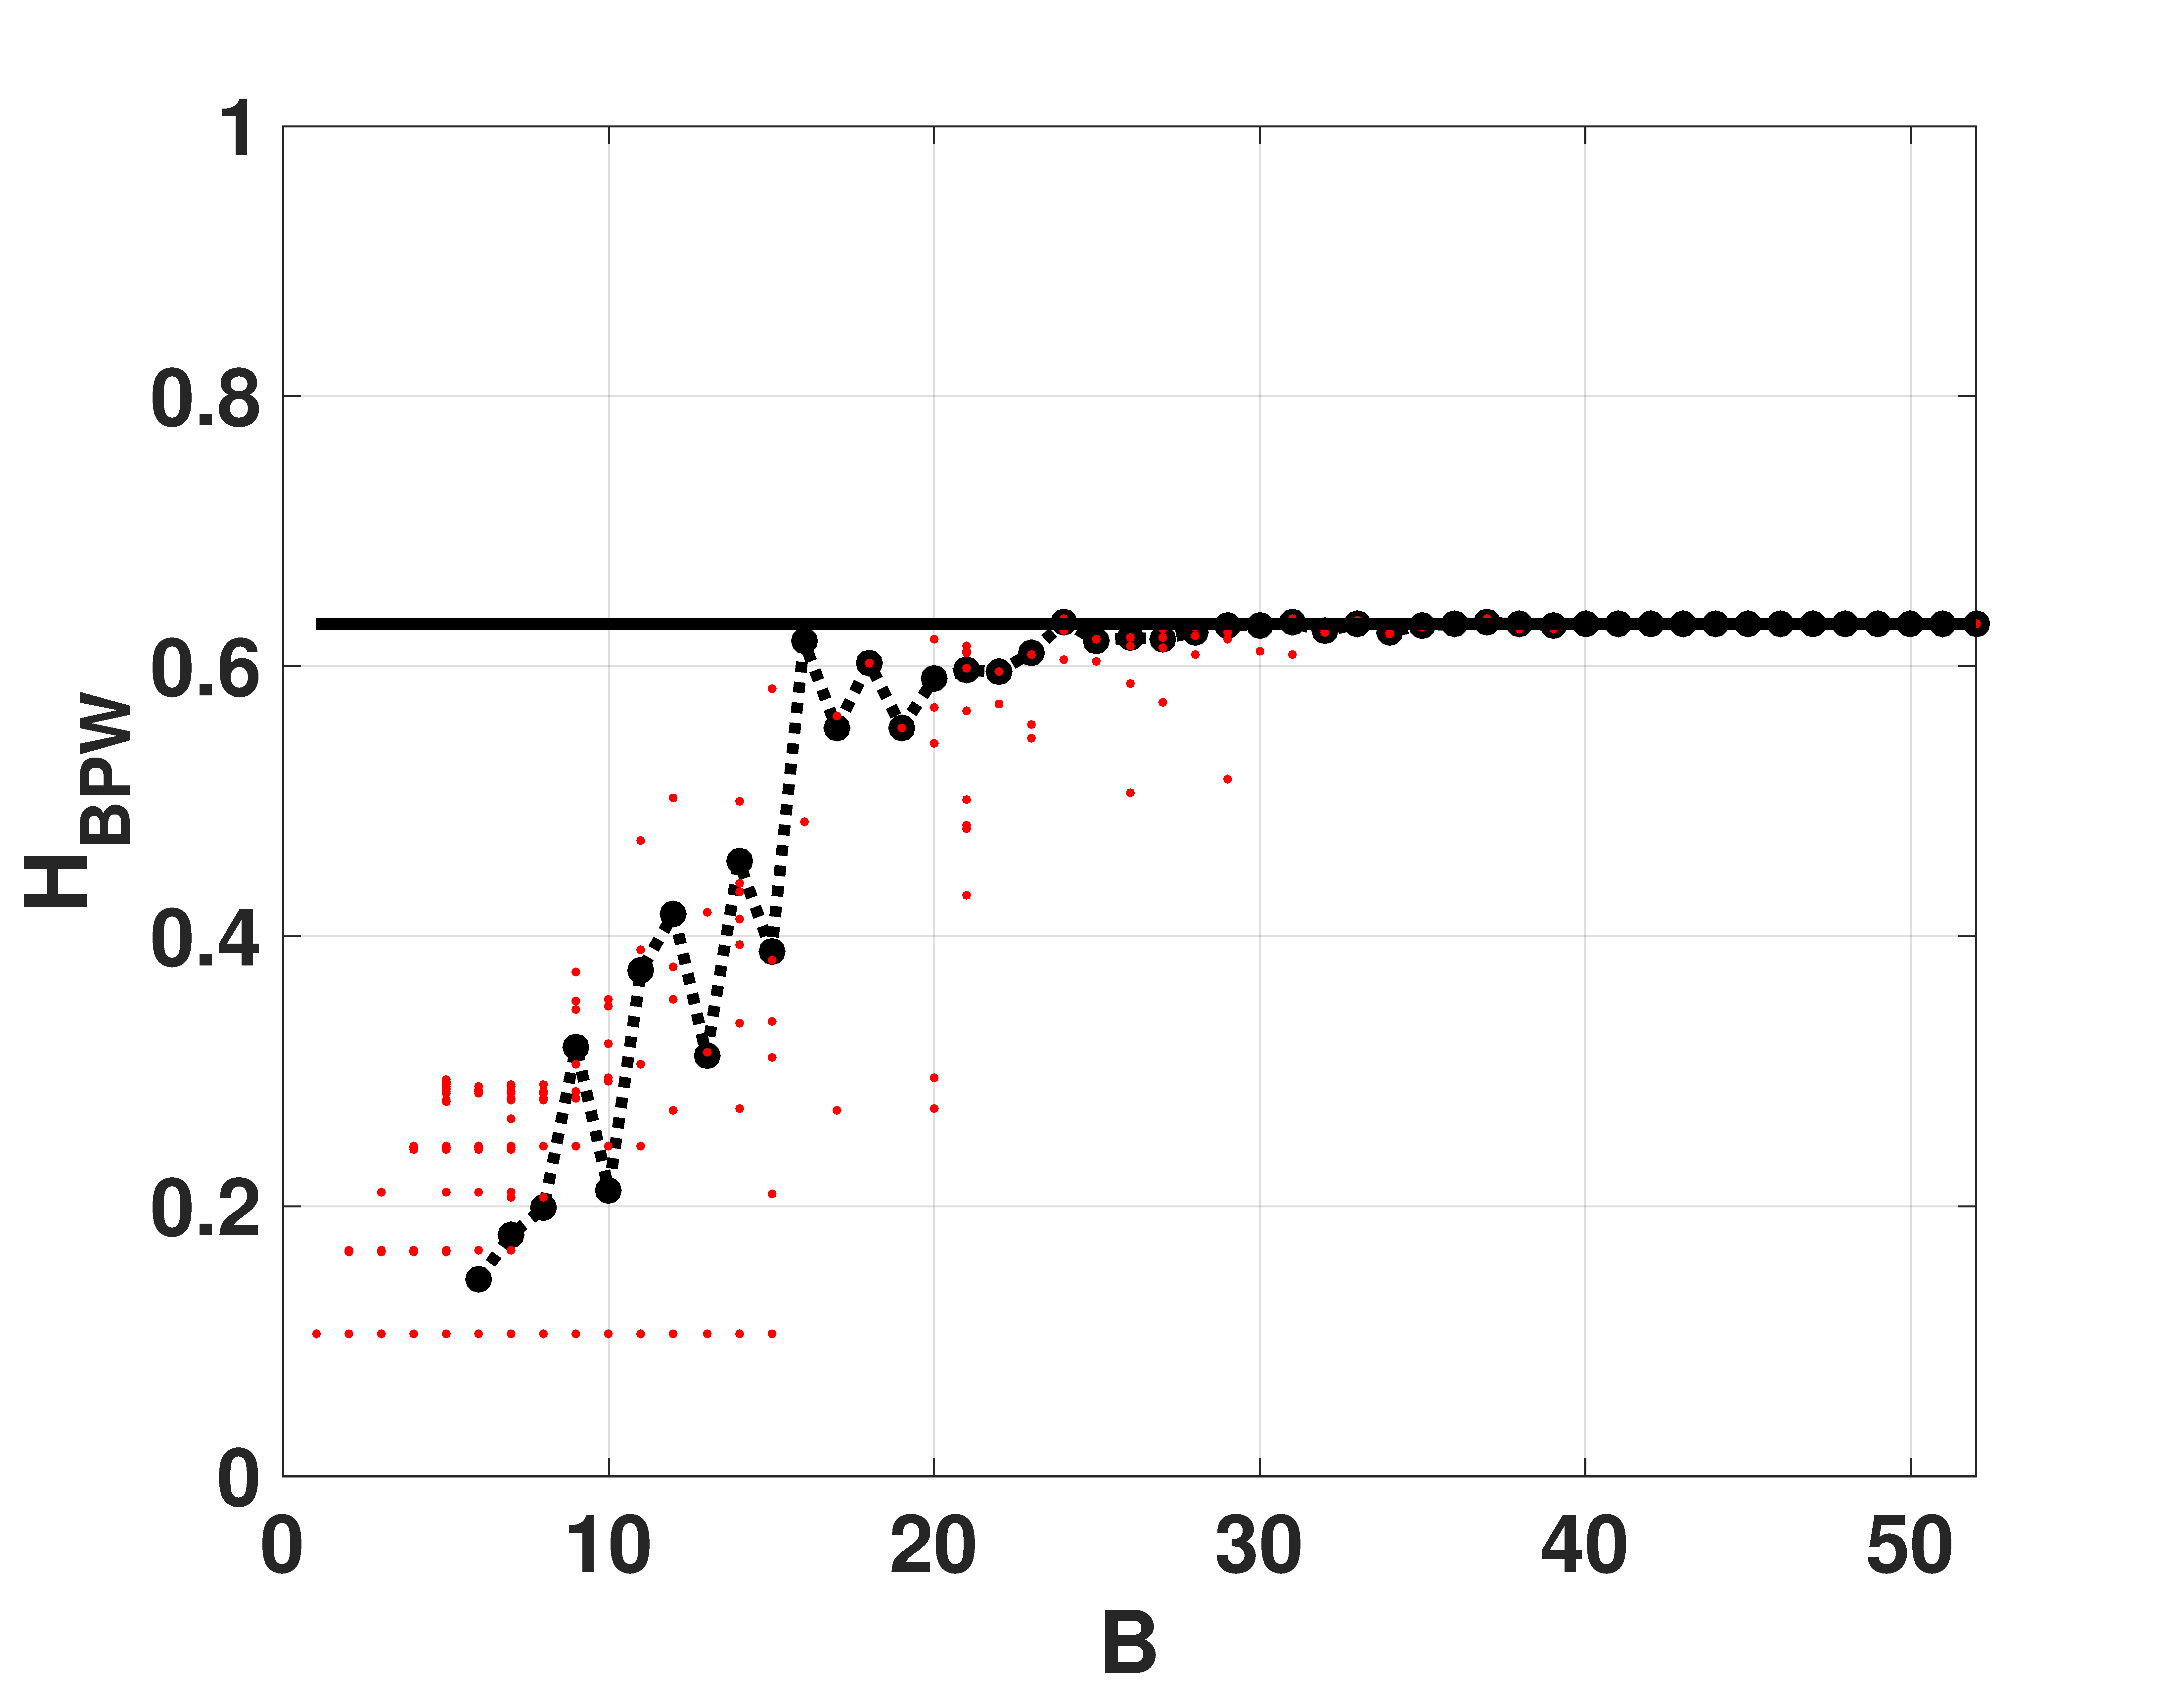
\includegraphics[width=.49\textwidth]{Hbpw_Switch}
	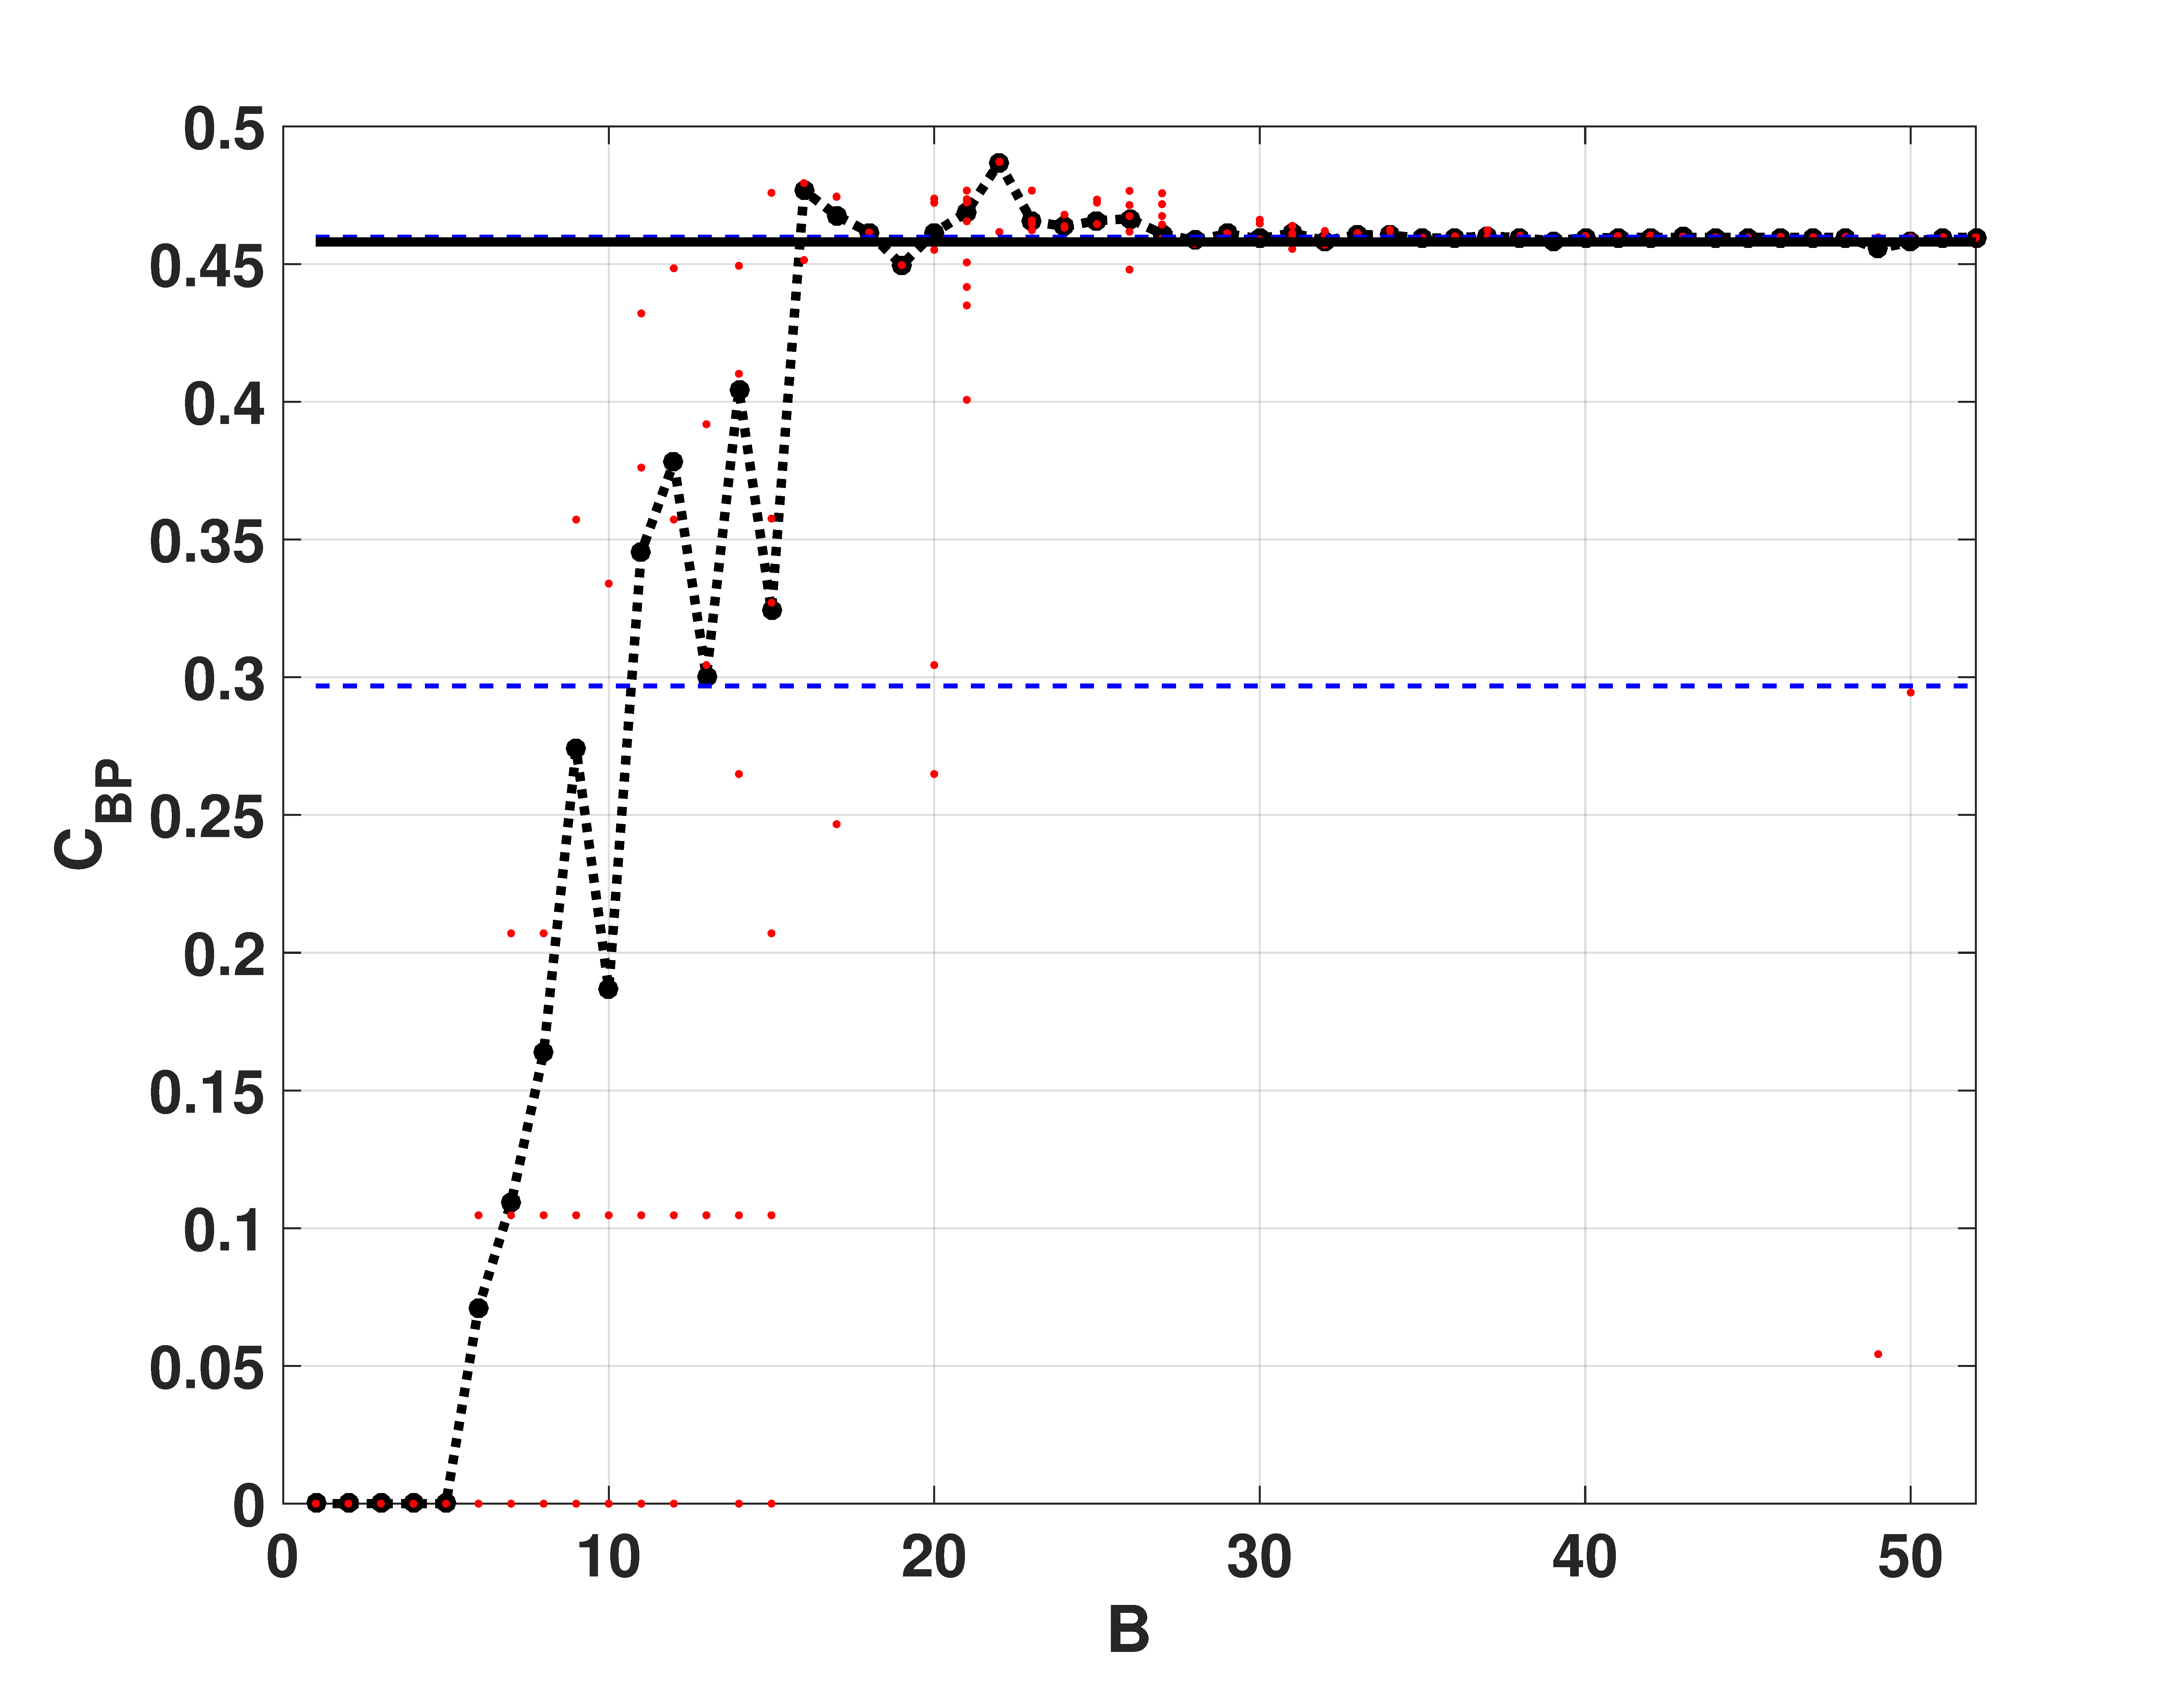
\includegraphics[width=.49\textwidth]{Cbp_Switch}
	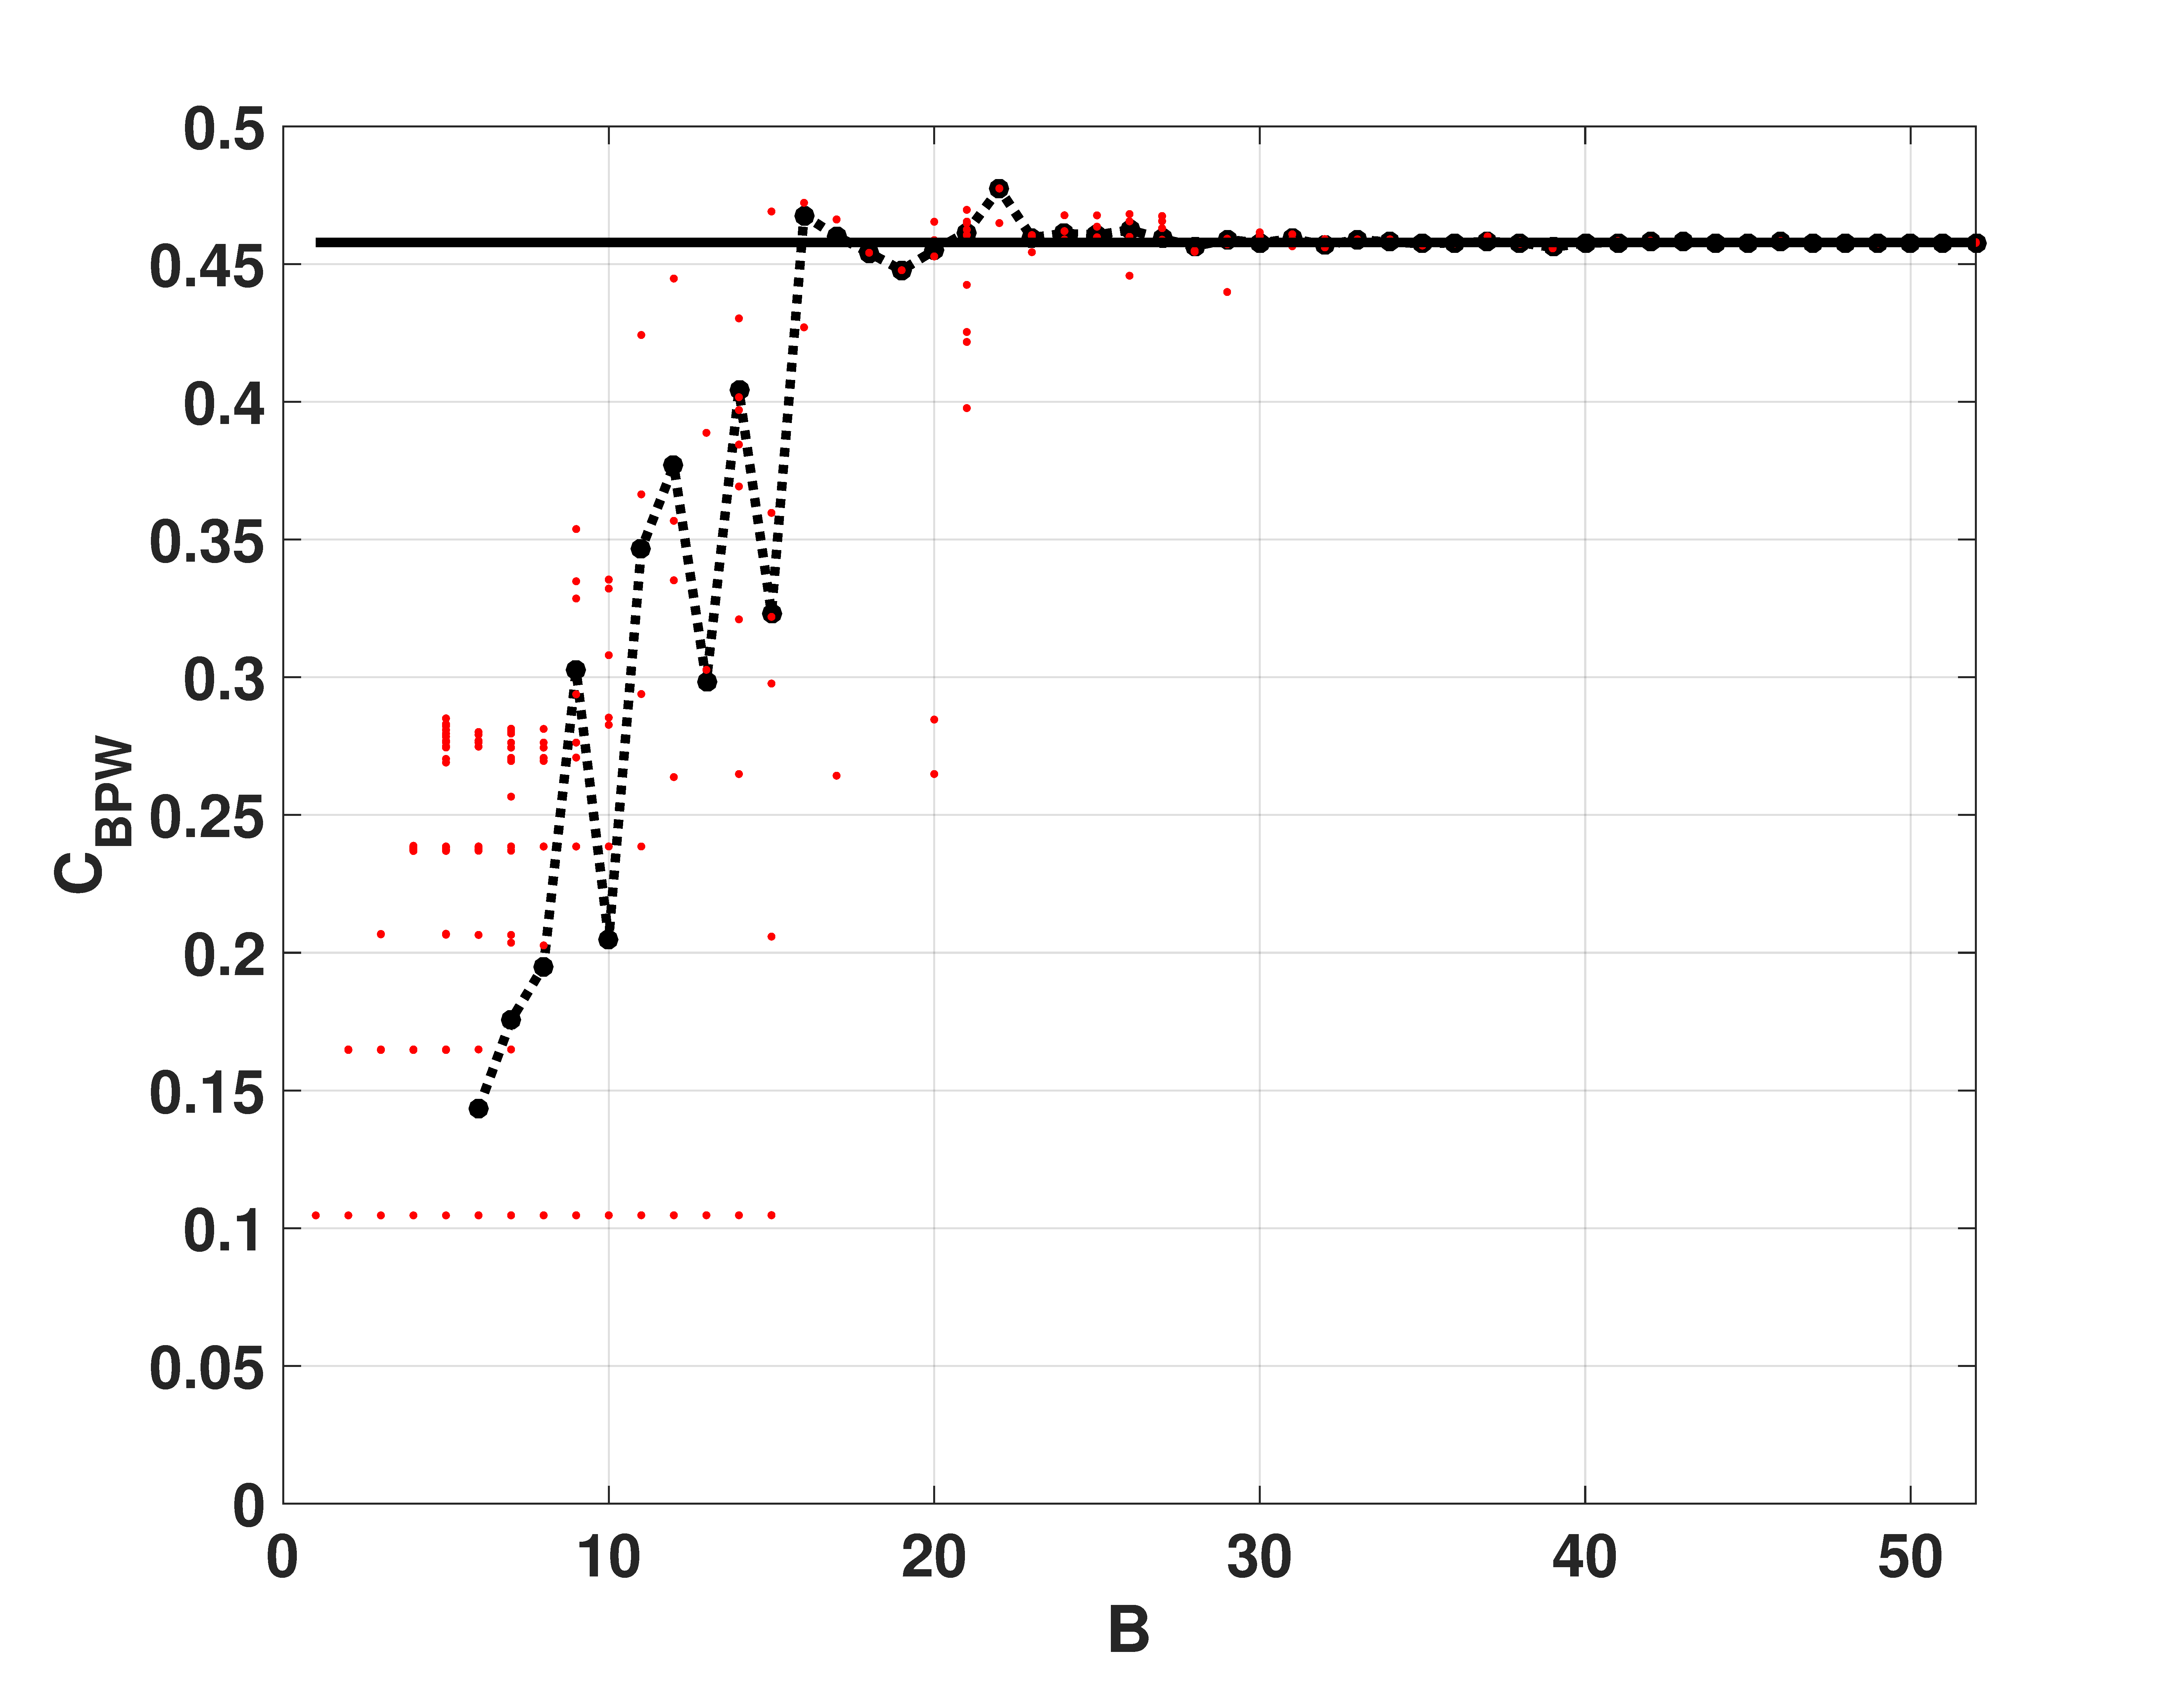
\includegraphics[width=.49\textwidth]{Cbpw_Switch}
	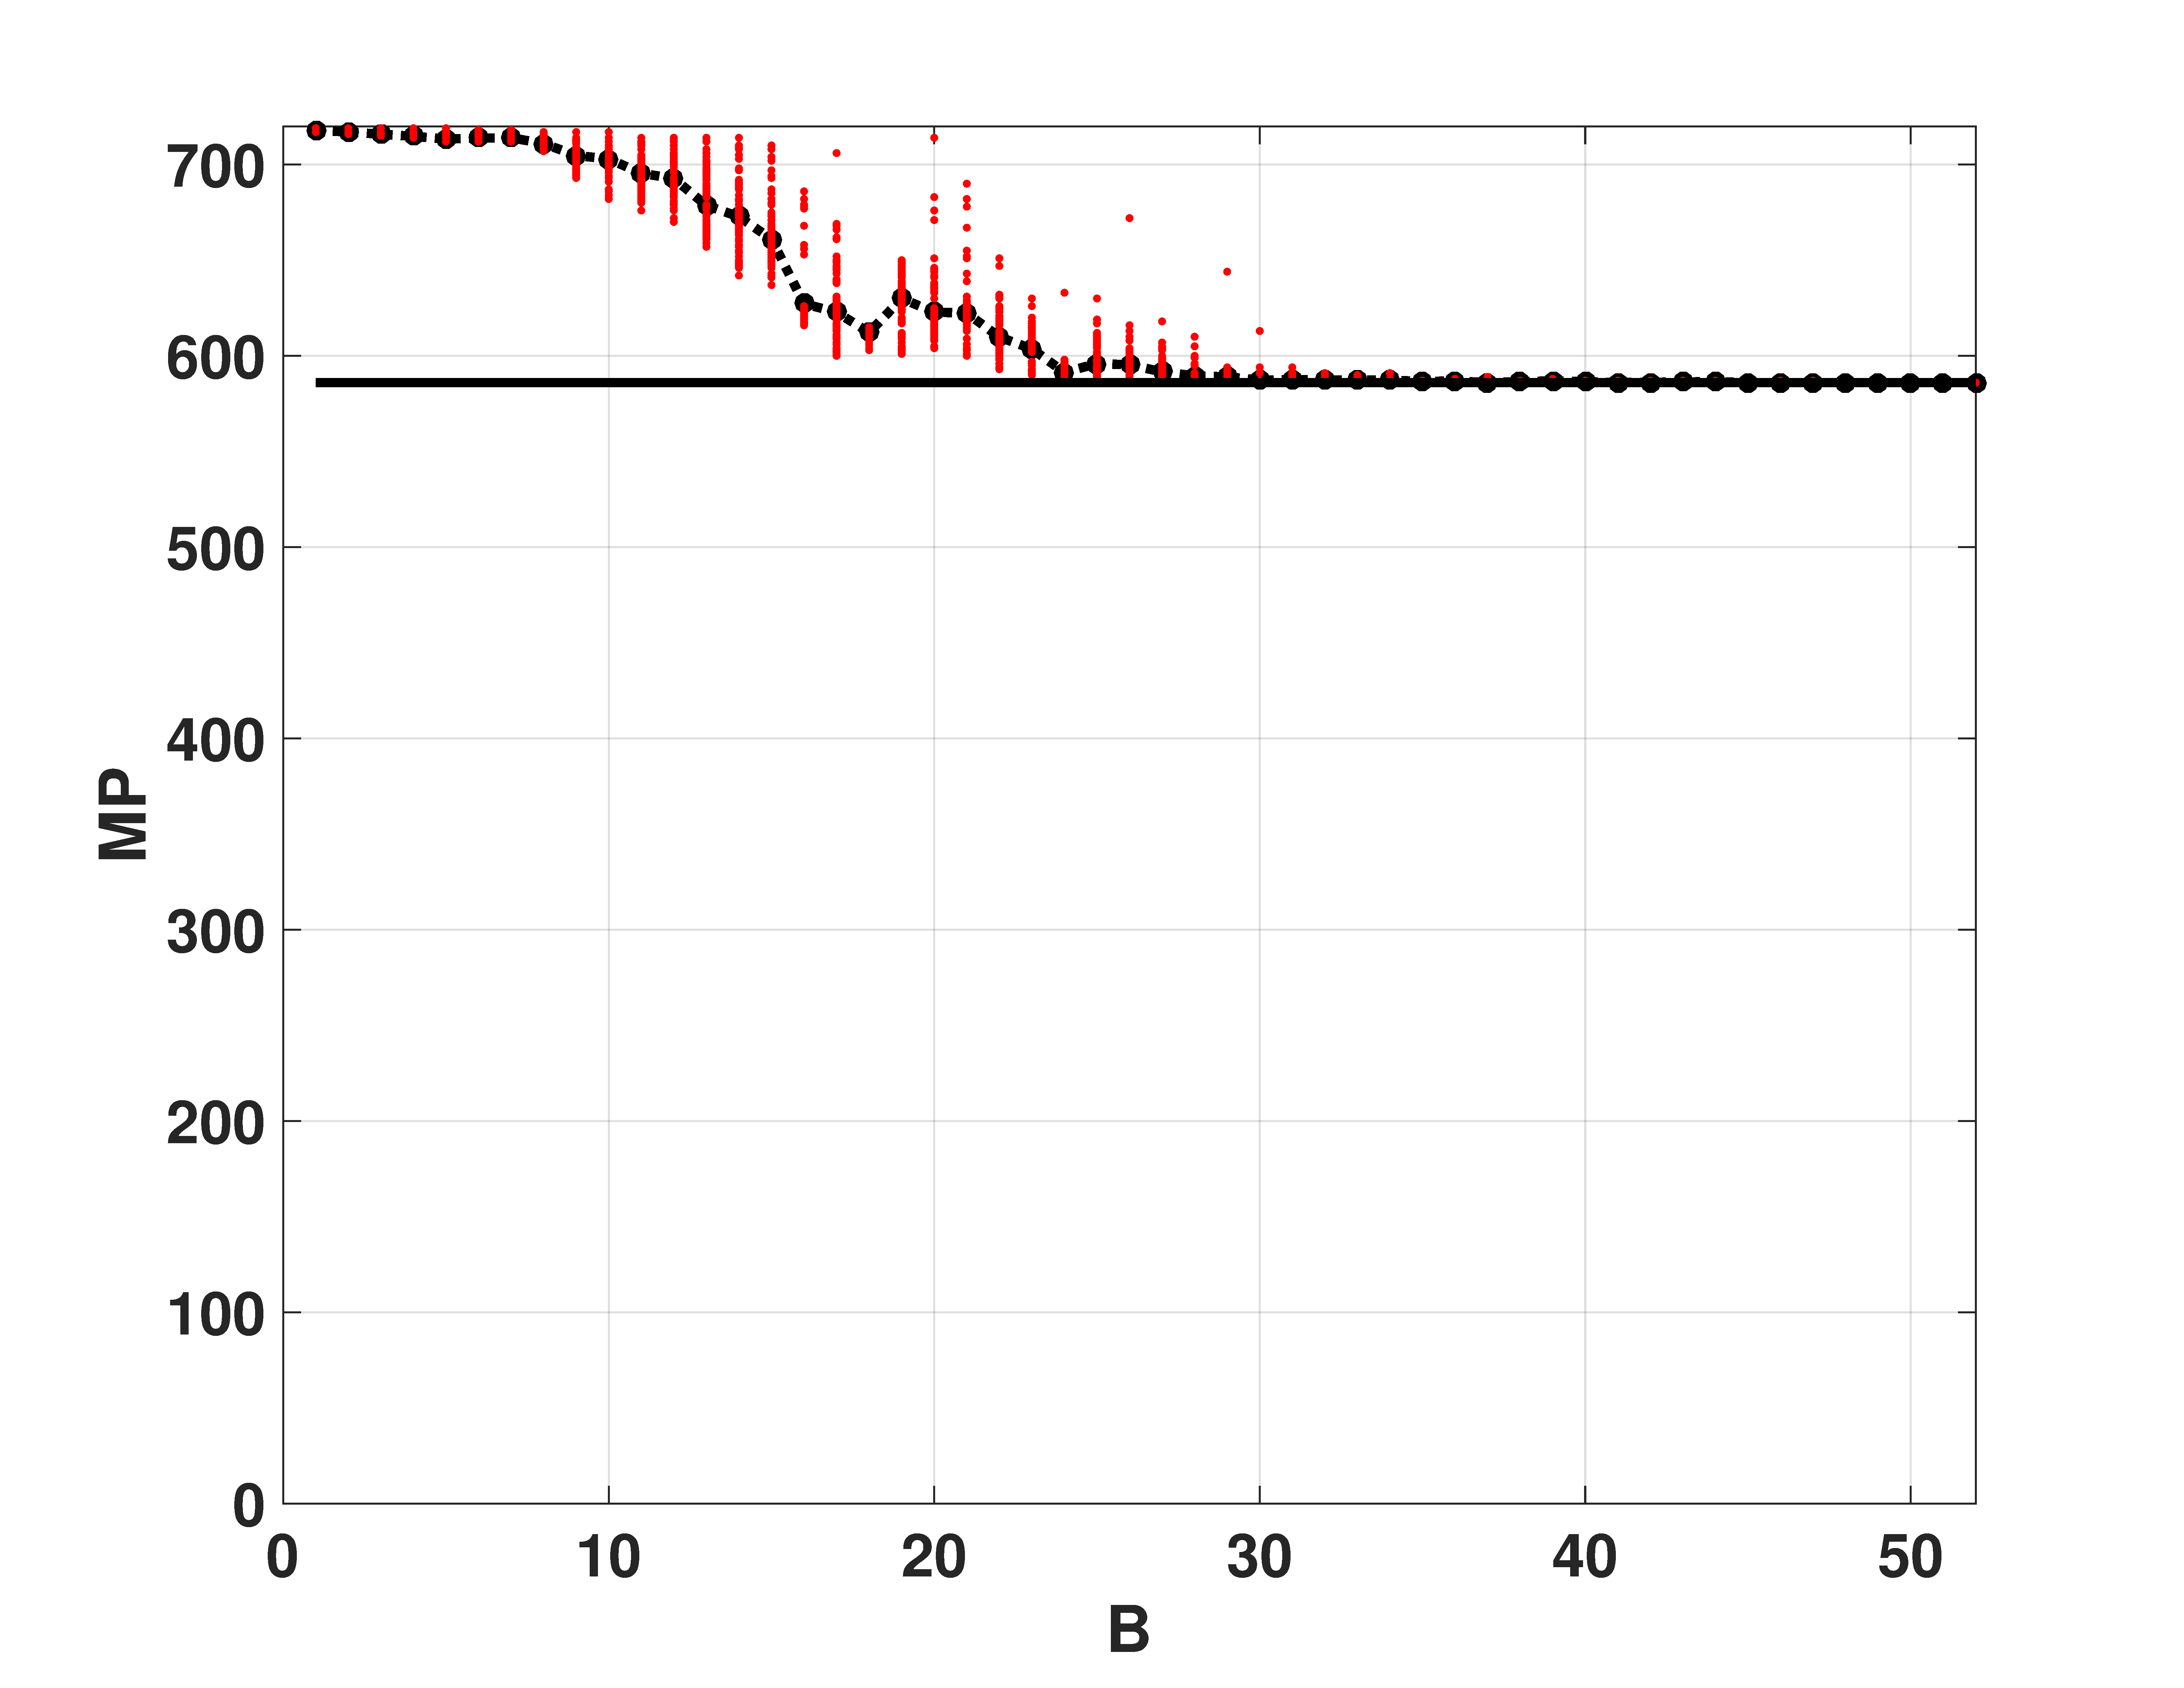
\includegraphics[width=.49\textwidth]{MP_Switch}
	\caption{Statistical properties of the SWITCH map (a) $H_{val}$ vs $B$ (b) $H_{BP}$ vs $B$ (c) $C_{BP}$ vs $B$ (d) $MP$ vs $B$.}
	\label{fig:SWITCH_QuantiB}
\end{figure}

Double entropy plane $H_{val}$ vs $H_{BP}$ is showed in Fig. \ref{fig:SWITCH_HH}.
The point reached in this plane for SWITCH map is similar to that reached for LOG map.
The mixing is slight better in this case.

\textcolor{red}{TENDRÍA QUE SACAR MAS CONCLUSIONES DE LOS PLANOS TENDRÍA QUE VERLAS EN LAS SERIES DE DATOS, ESPECIALMENTE EL PUNTO ESE QUE DA CORRIDO}

\begin{figure}
	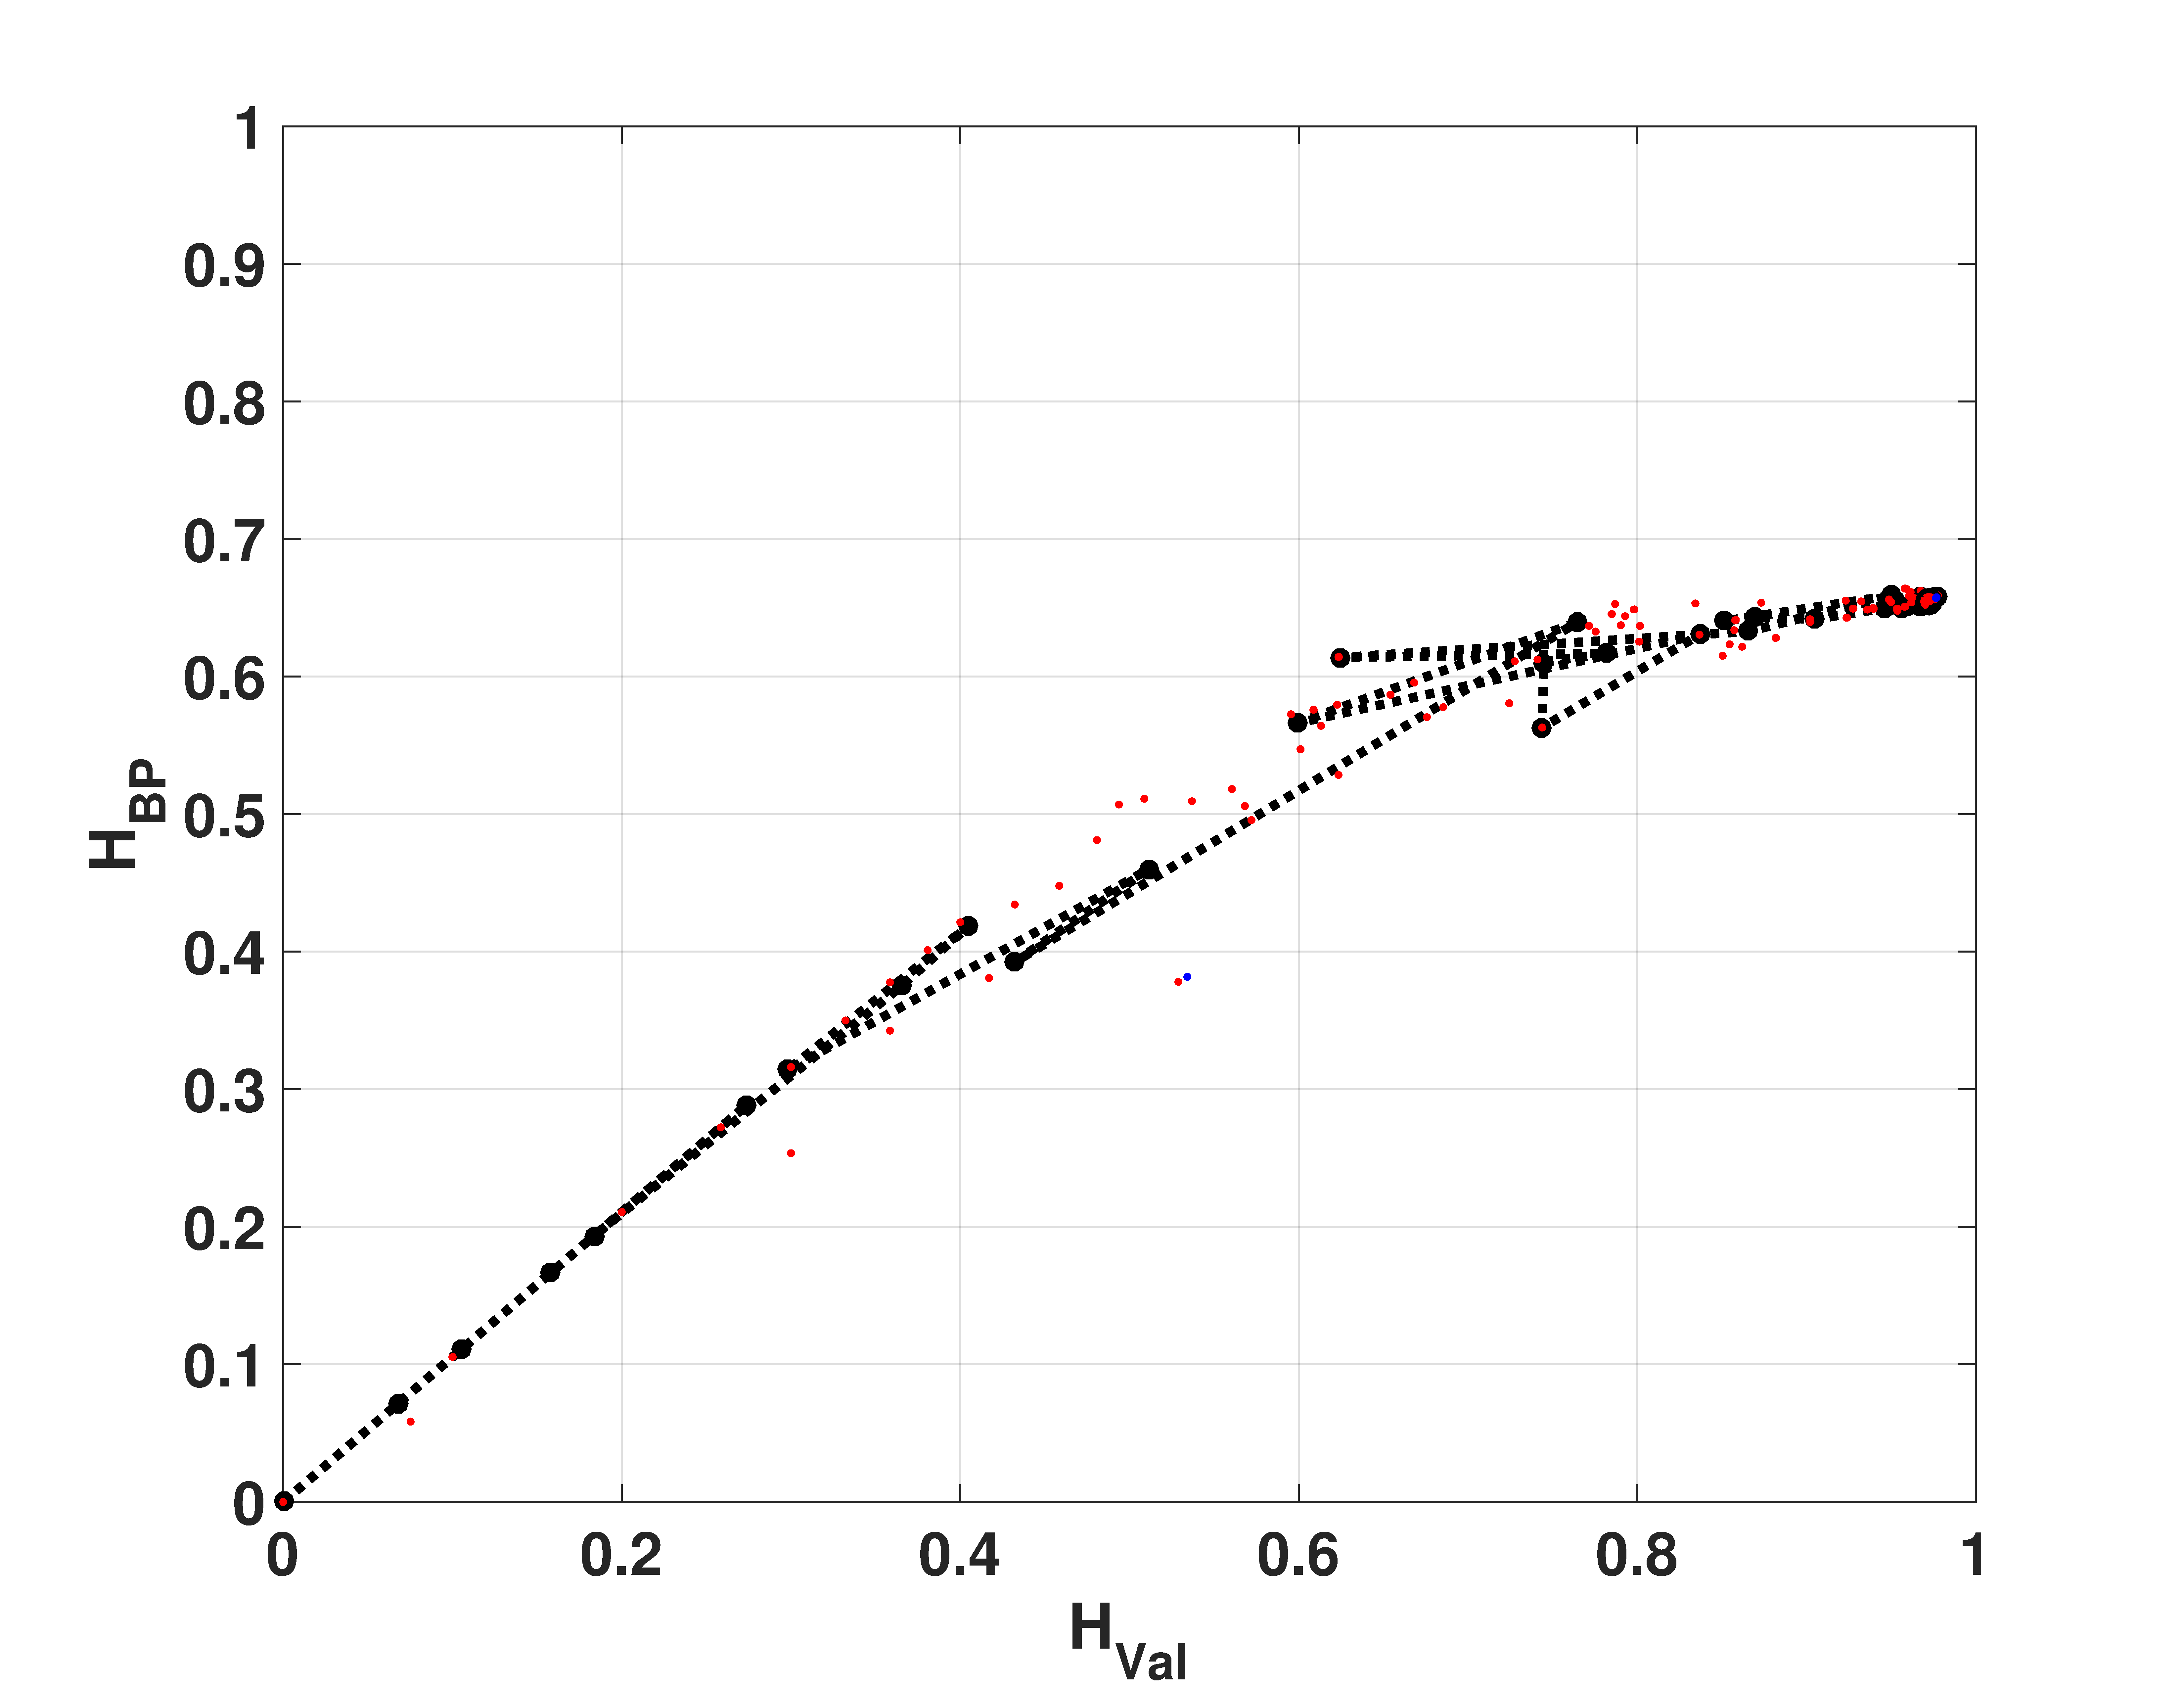
\includegraphics[width=.49\textwidth]{HbpHval_Switch}
	\caption{Evolution of statistical properties in double entropy plane of SWITCH map using binary representation: (a) $H_{val}$ vs $H_{BP}$ (b) $H_{val}$ vs $H_{BPW}$.}
	\label{fig:SWITCH_HH}
\end{figure}

Entropy-complexity plane $C_{BP}$ vs $H_{BP}$ is showed in Fig. \ref{fig:SWITCH_HC}.
If we compare with the same plane in the case of LOG (Fig. \ref{fig:LOG_HC}. a.), $C_{BP}$ is lower for SWITCH, this fact shows a more random behaviour.

\begin{figure}
	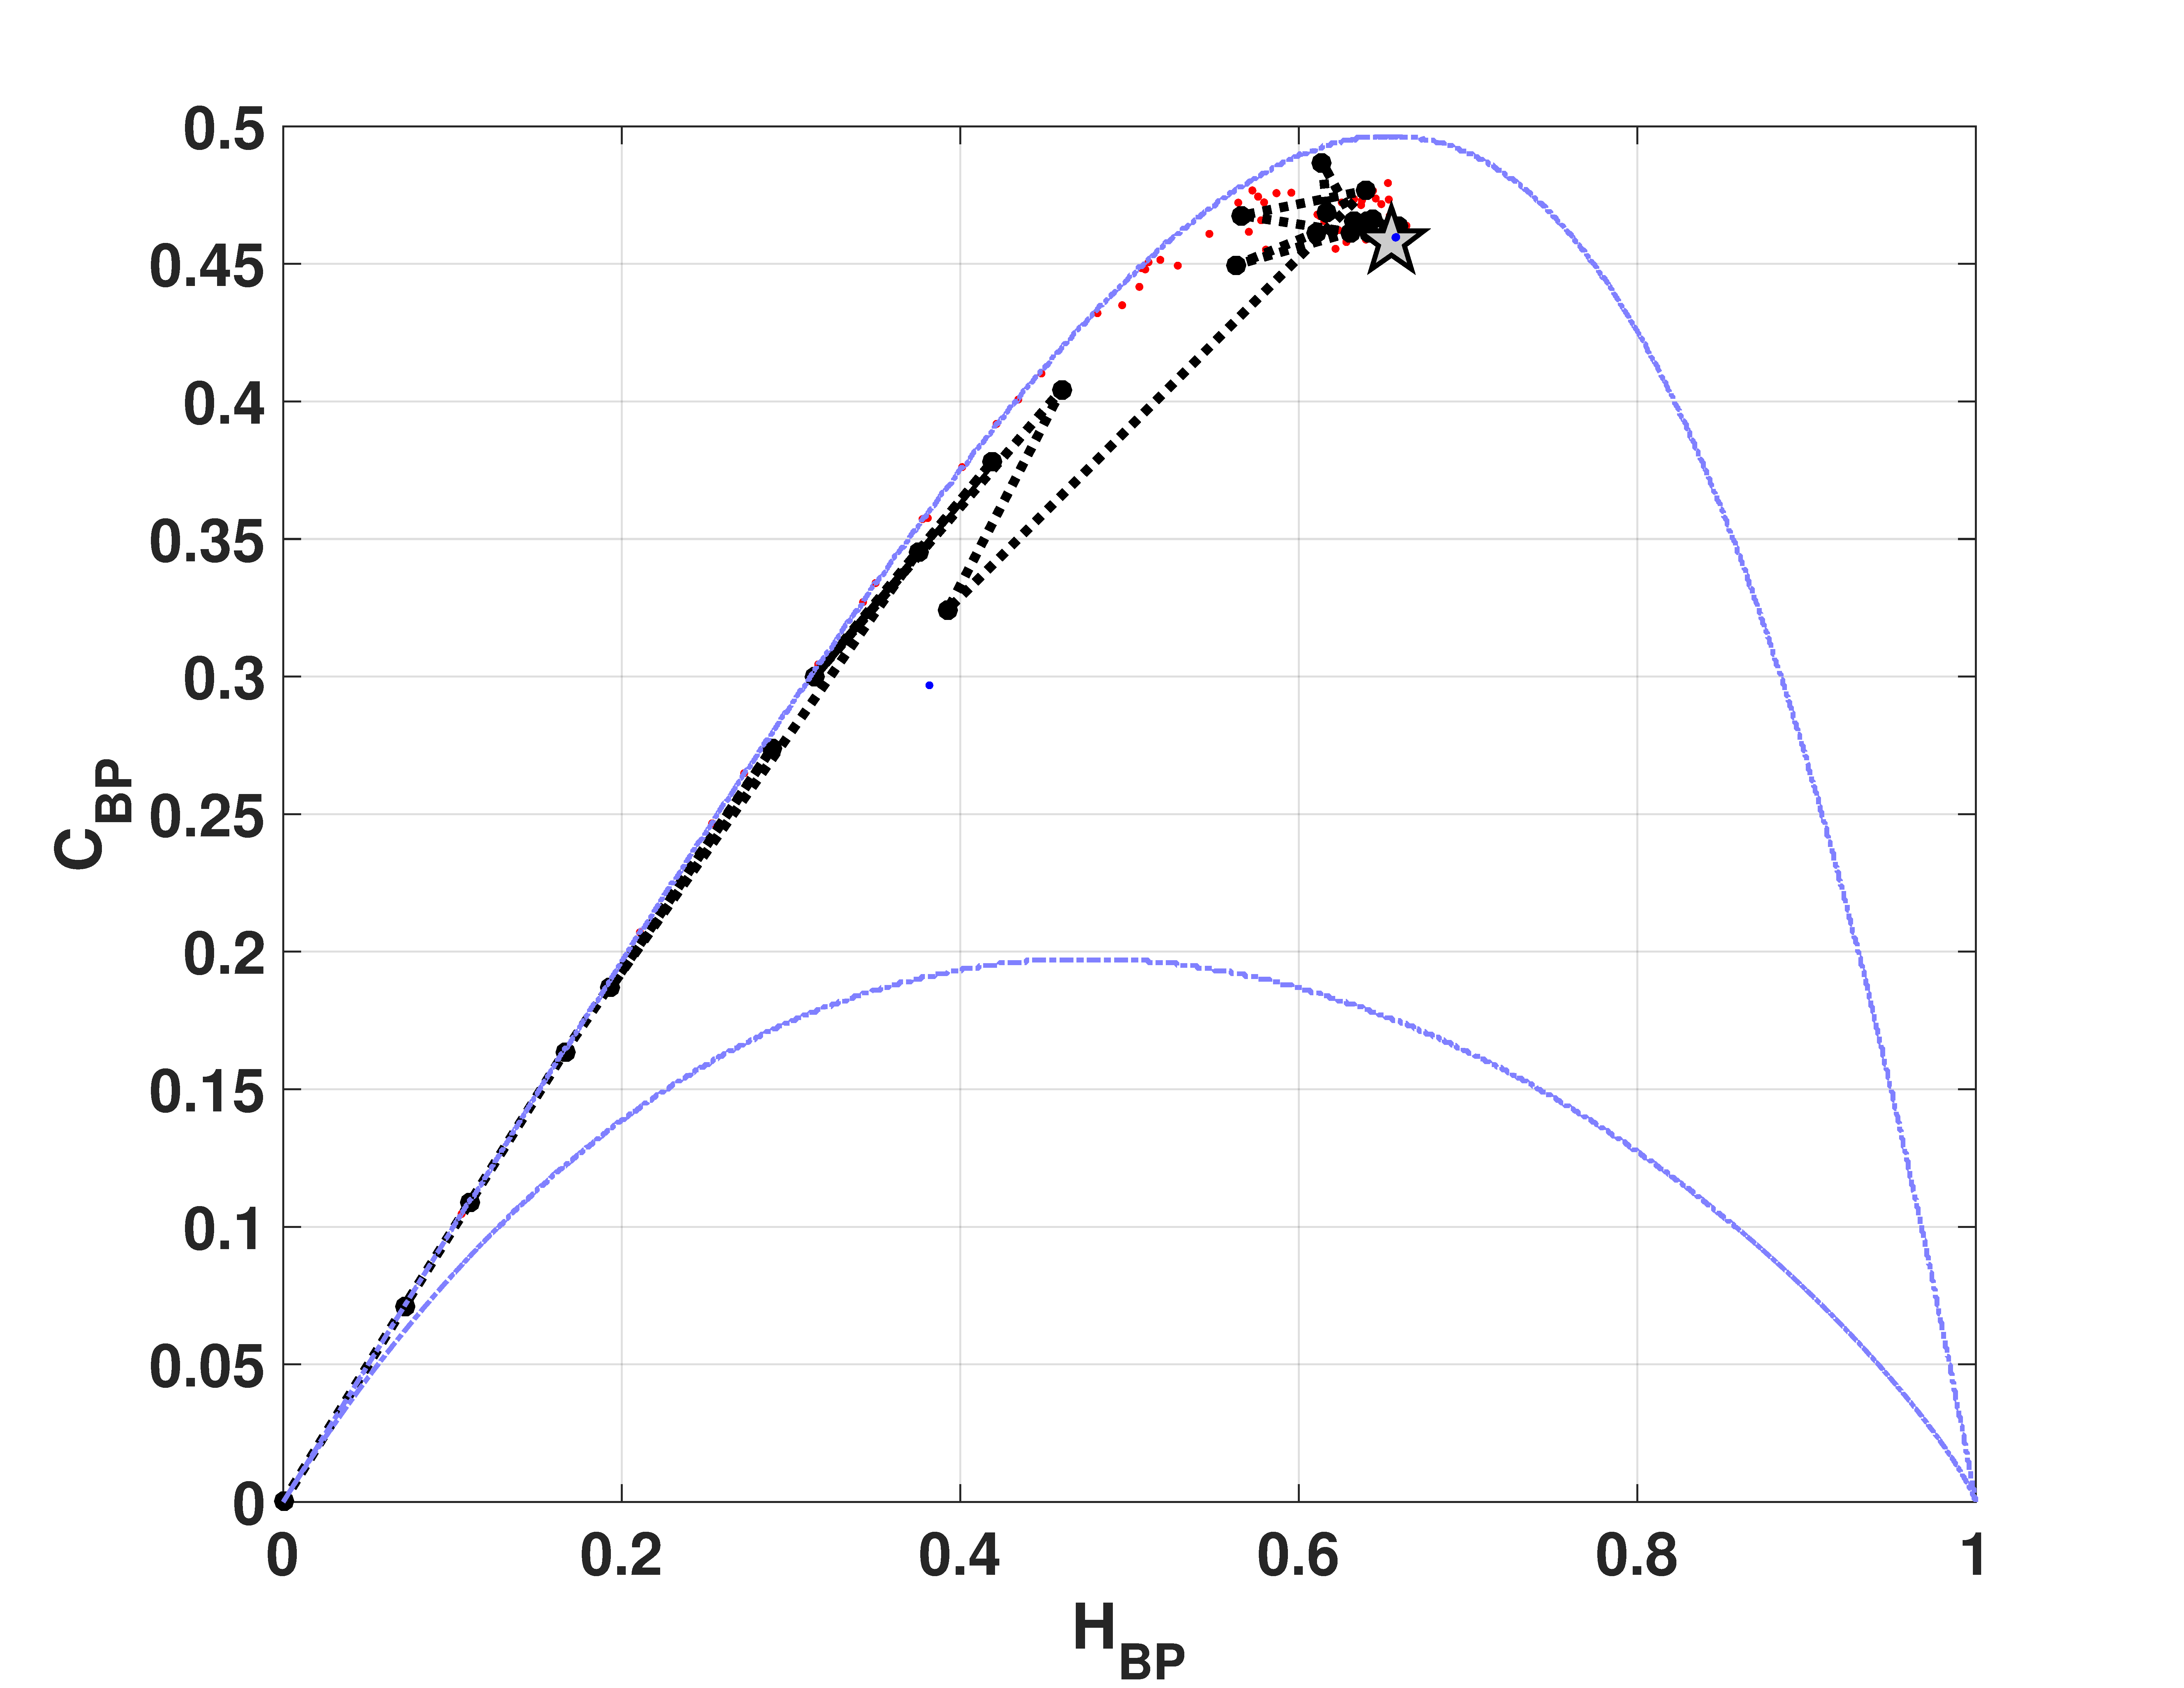
\includegraphics[width=.49\textwidth]{CbpHbp_Switch}
	\caption{Evolution of statistical properties in entropy-complexity plane of SWITCH map: $C_{BP}$ vs $H_{BP}$.}
	\label{fig:SWITCH_HC}
\end{figure}

\subsubsection{EVEN and ODD} \label{sssec:skipp}

In Figures \ref{fig:Hval_Even} and \ref{fig:Hval_Odd} we can see that quantifiers related to the normalized histogram of values slightly degrades with the skipping procedure.
For example $\left\langle H_{hist}\right\rangle $ reduces from $0.9722$ without skipping to $0.9459$ for EVEN and $0.9706$ for ODD. 
This difference between EVEN and ODD in floating point is because a high dispersion was obtained for $H_{hist}$, $H_{BP}$ and $C_{BP}$ but not for $H_{BPW}$ or $C_{BPW}$.

Figures \ref{fig:Hbp_Even} to \ref{fig:MP_Even} and Figures \ref{fig:Hbp_Odd} to \ref{fig:MP_Odd} show the results of BP and BPW quantifiers for EVEN and ODD respectively.
Higher accuracy is required to achieve lower complexity than without using skipping.
From the MP point of view a great improvement is obtained using any of the skipping strategies but ODD is slightly better than EVEN.
Missing patterns are reduced to $MP = 118$ for EVEN and ODD, increasing the maximum allowed Bandt \& Pompe entropy that reaches the mean value $\left\langle H_{BP}\right\rangle  = 0.8381$ for EVEN, and $\left\langle H_{BP}\right\rangle  = 0.9094$.
The complexity is reduced to $\left\langle C_{BP}\right\rangle = 0.224$ for EVEN and $\left\langle C_{BP}\right\rangle = 0.282$ for ODD.
The minimum number of bits to converge to this value is $B>40$ for both EVEN and ODD maps.
%
\begin{figure}[H]
	\centering
	\begin{subfigure}[b]{0.49\textwidth}
		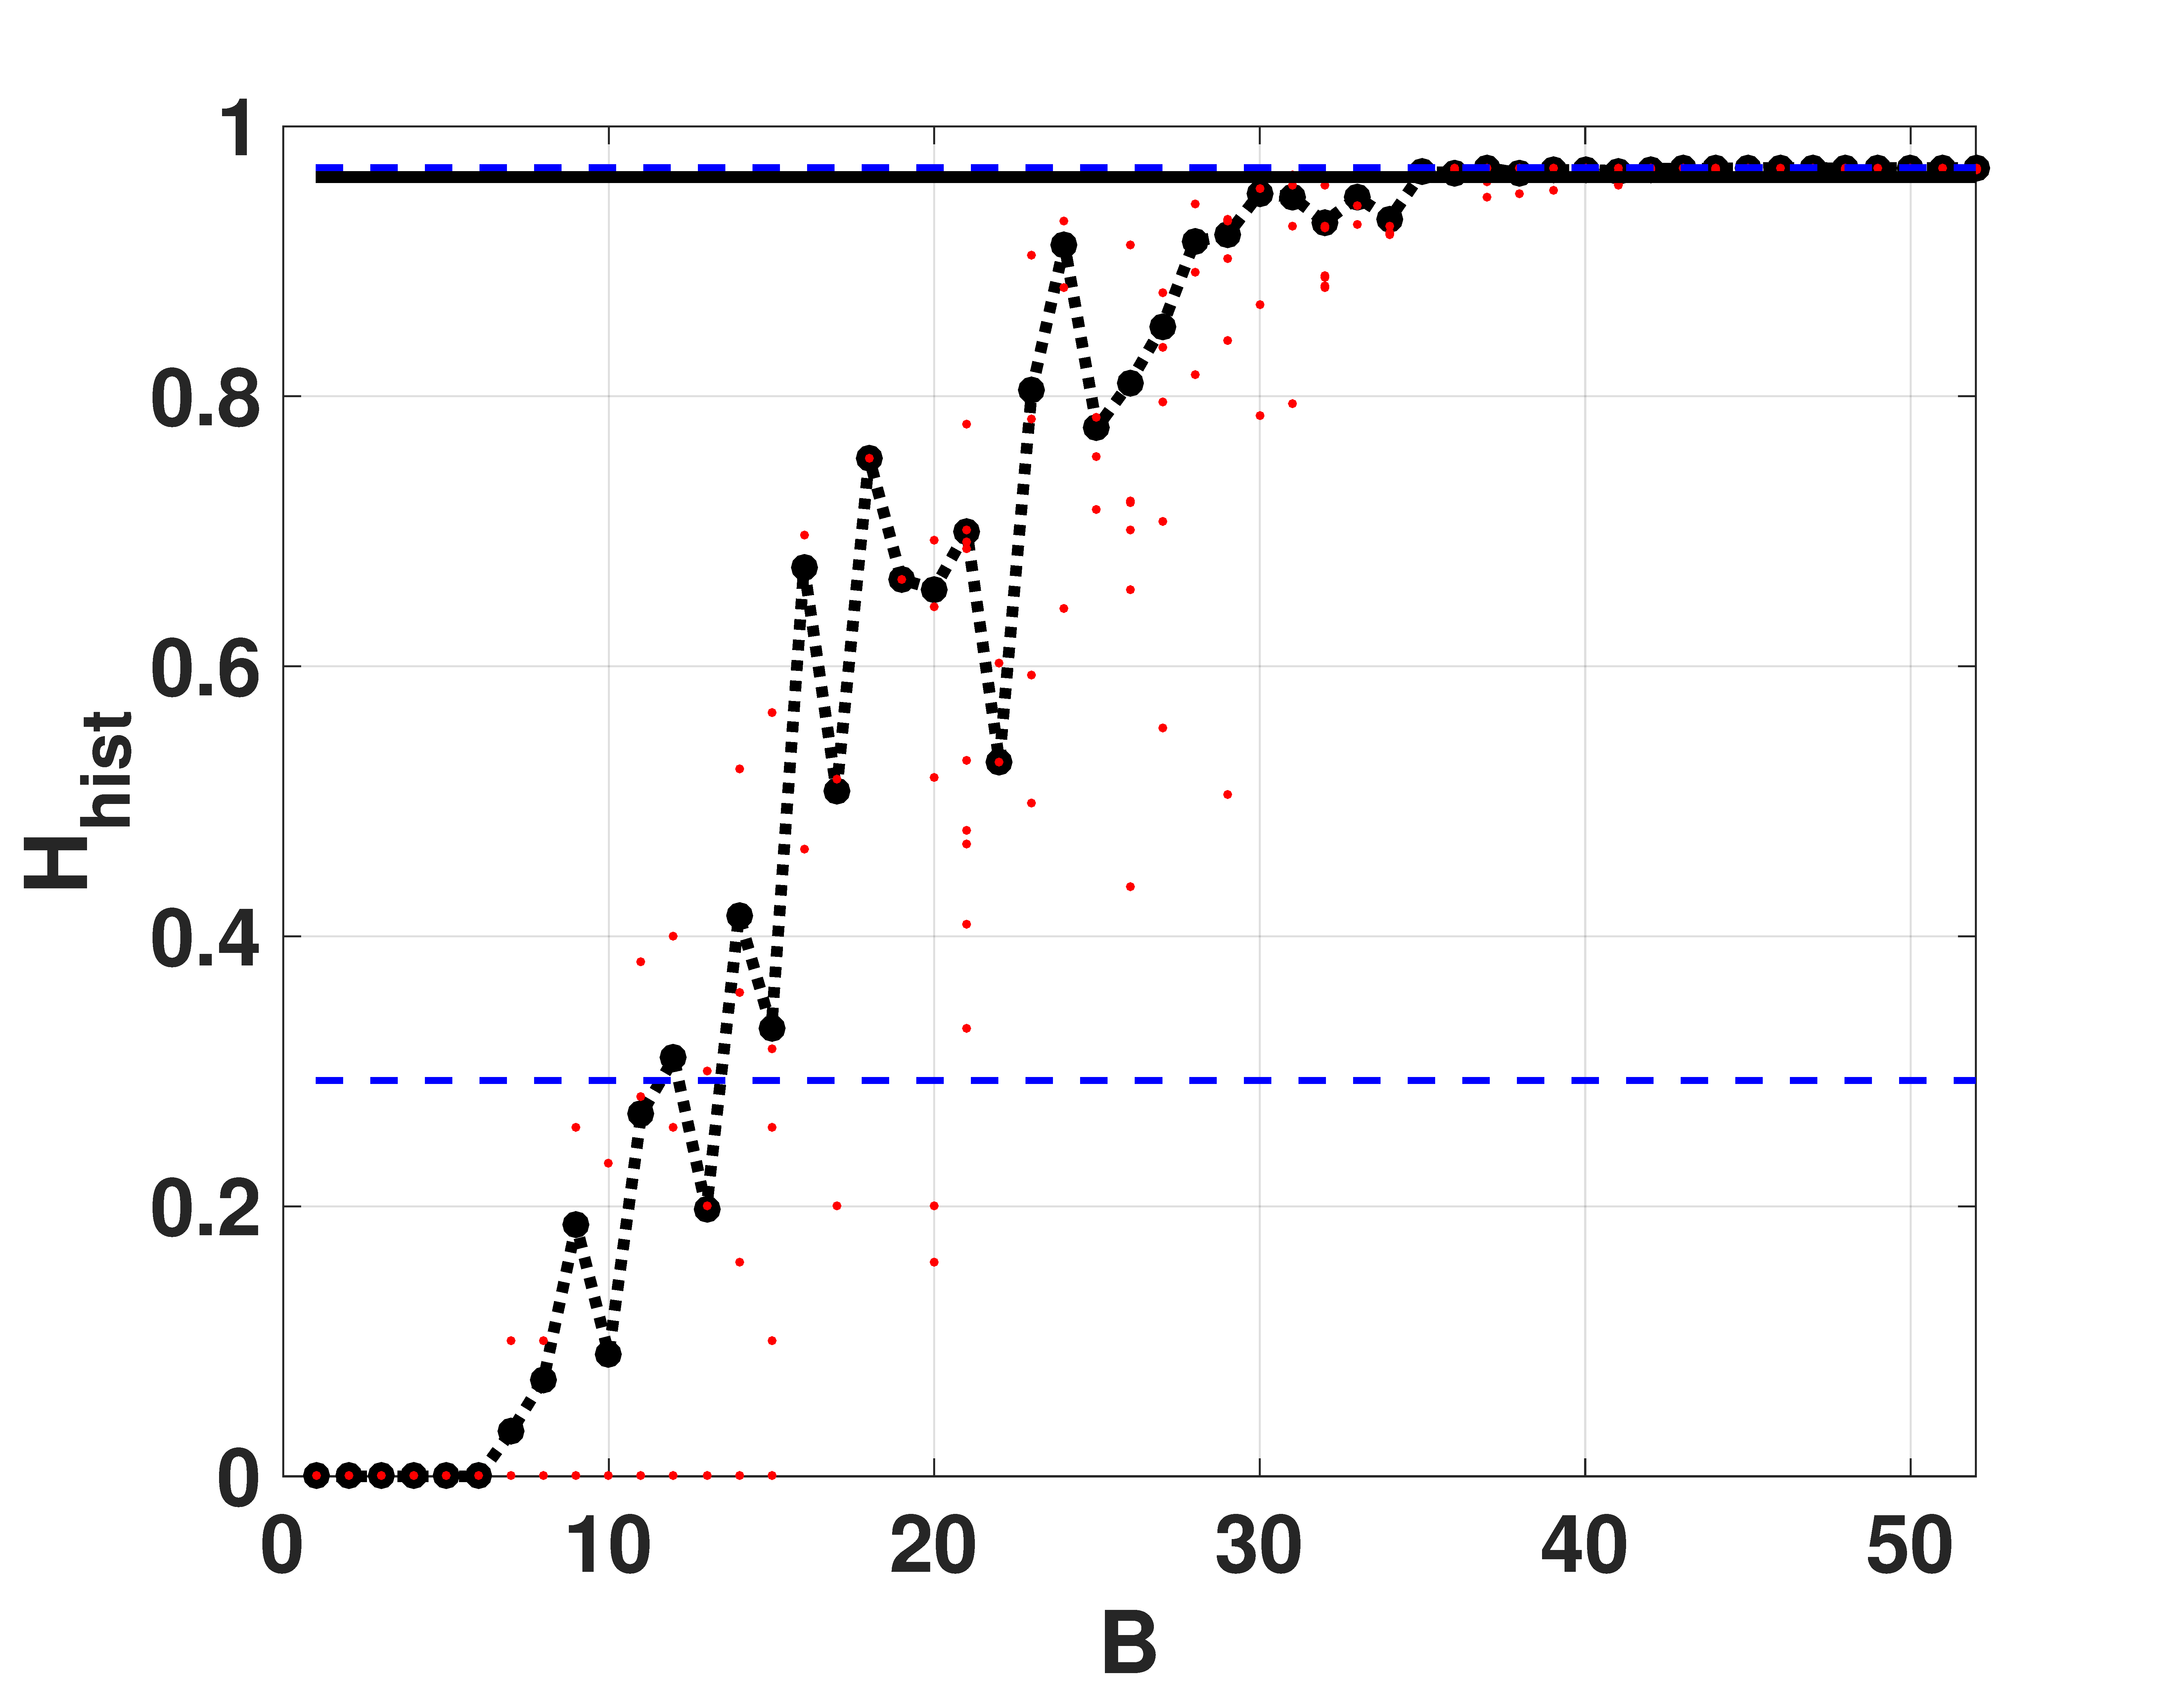
\includegraphics[width=\textwidth]{Hval_Even}
		\caption{$H_{hist}$ vs. $B$}
		\label{fig:Hval_Even}
	\end{subfigure}
	\begin{subfigure}[b]{0.49\textwidth}
		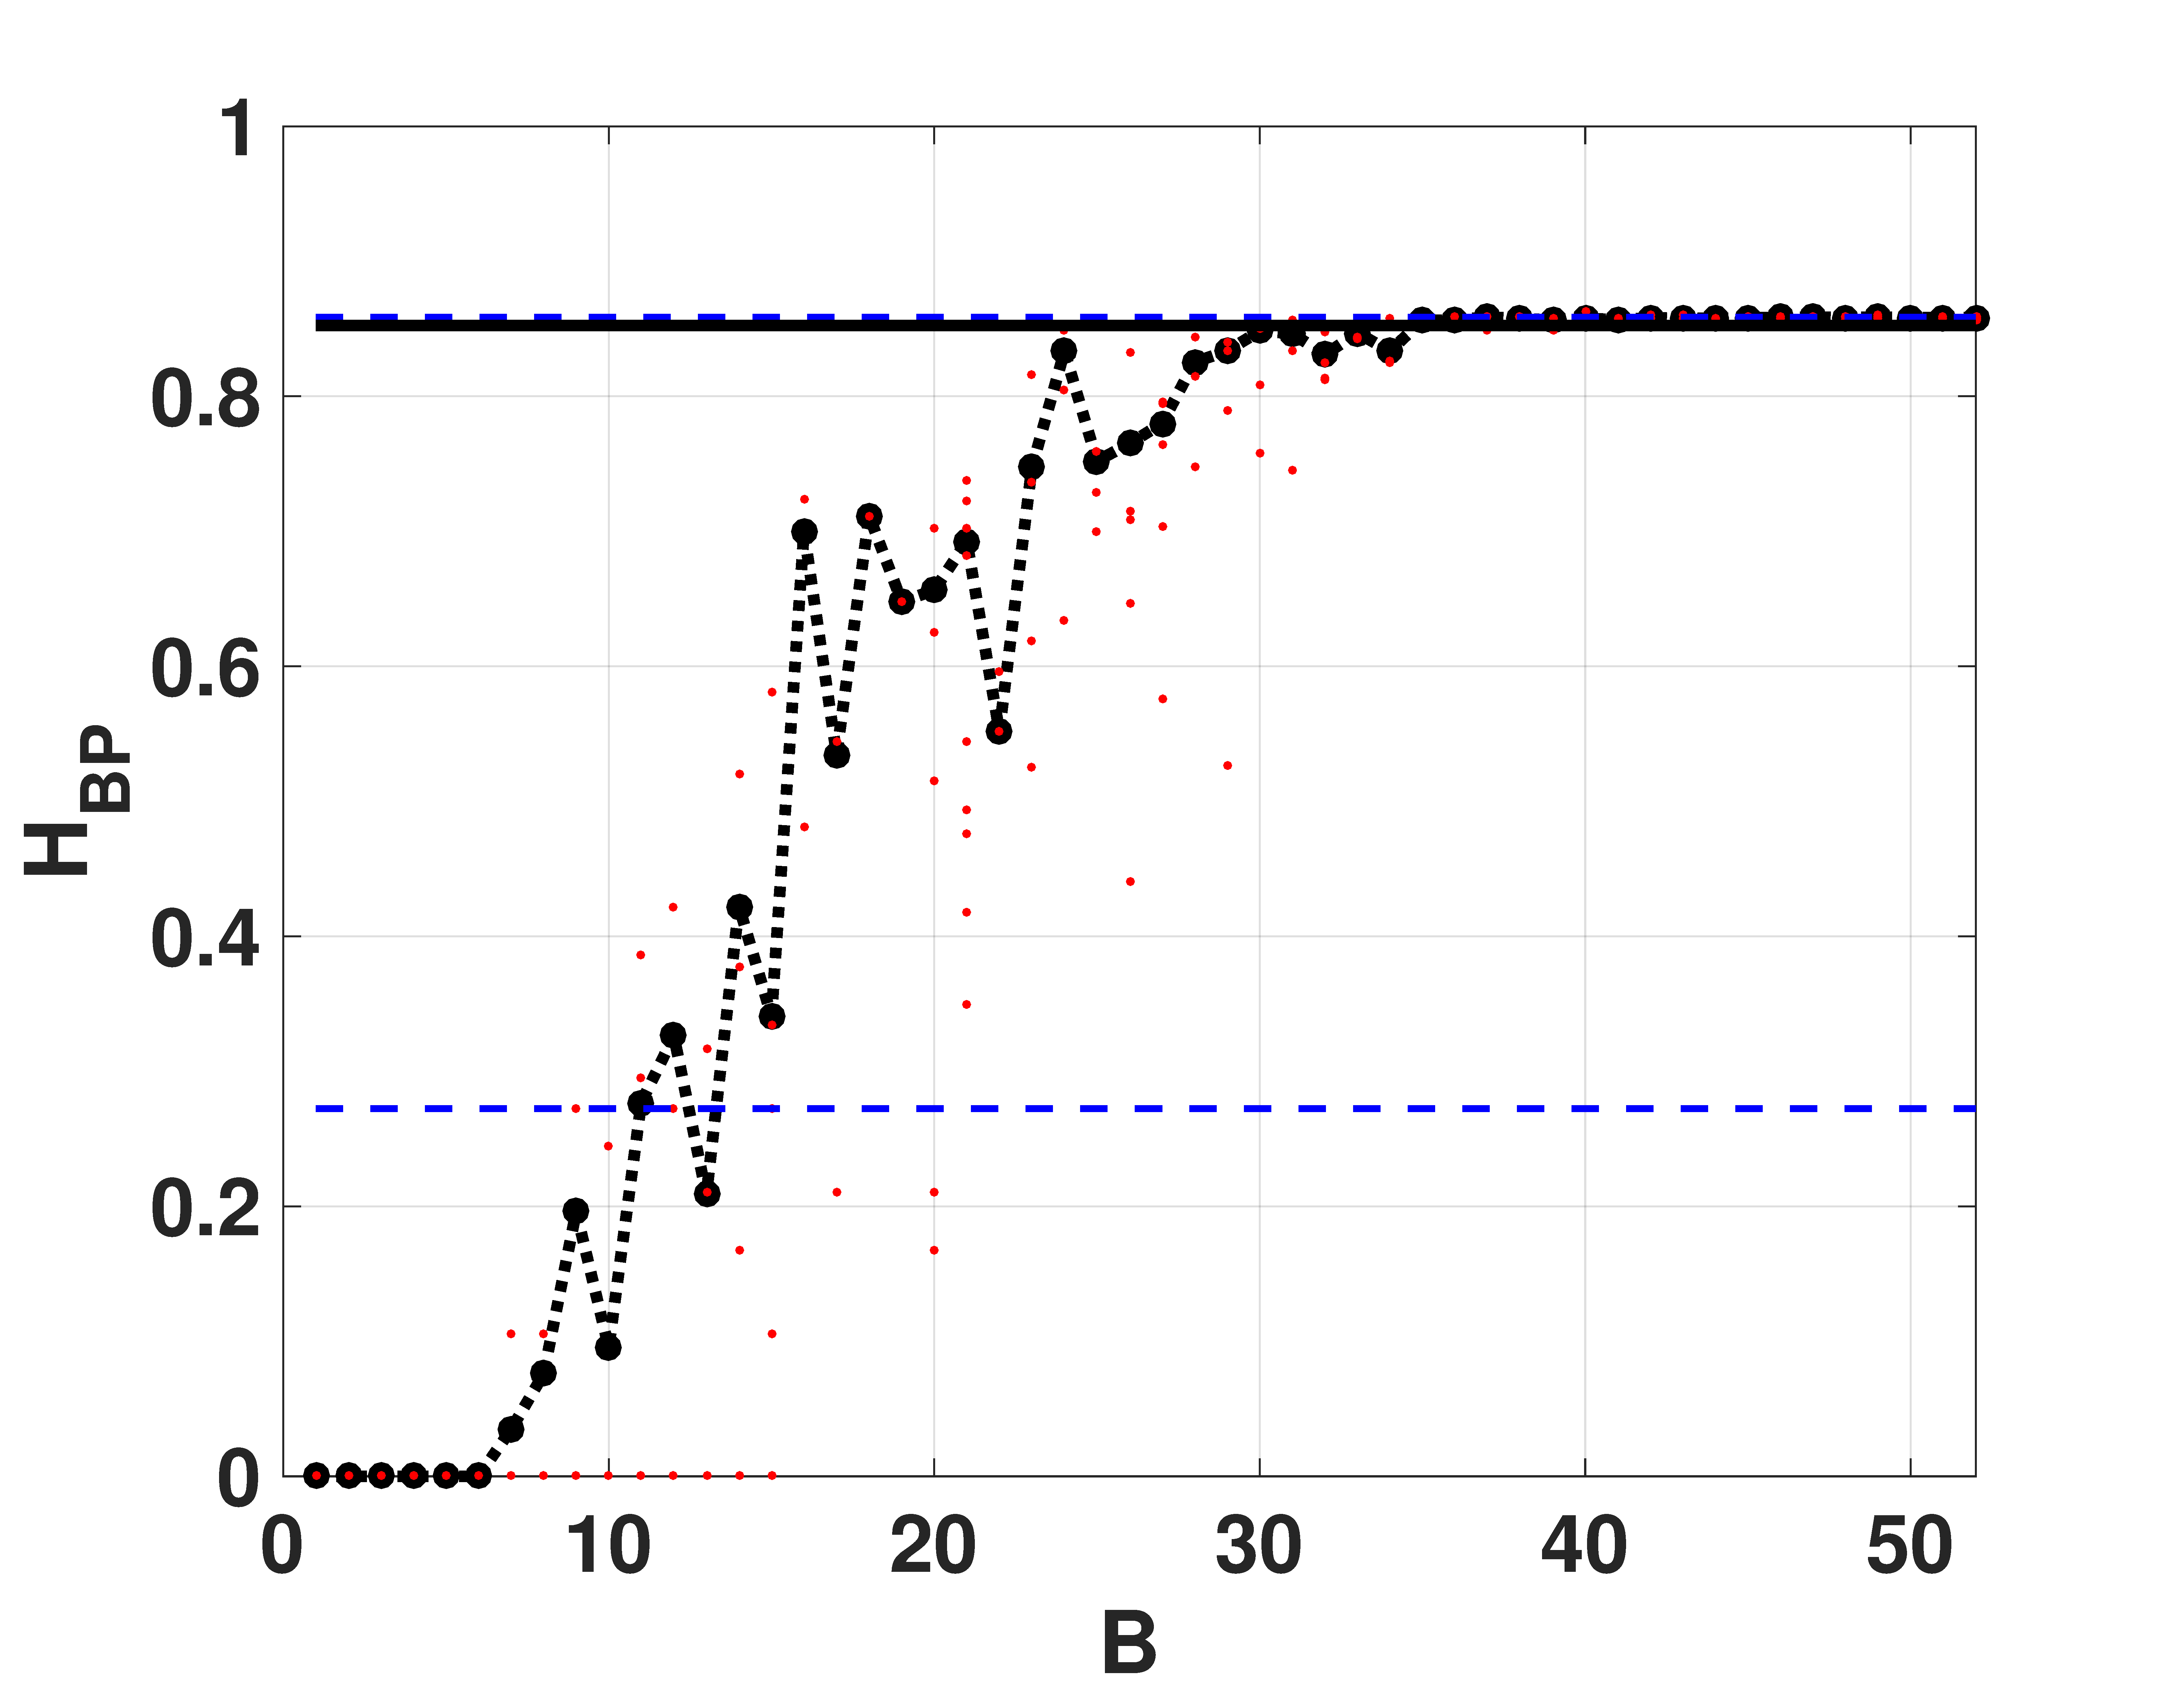
\includegraphics[width=\textwidth]{Hbp_Even}
		\caption{$H_{BP}$ vs. $B$}
		\label{fig:Hbp_Even}
	\end{subfigure}
	\begin{subfigure}[b]{0.49\textwidth}
		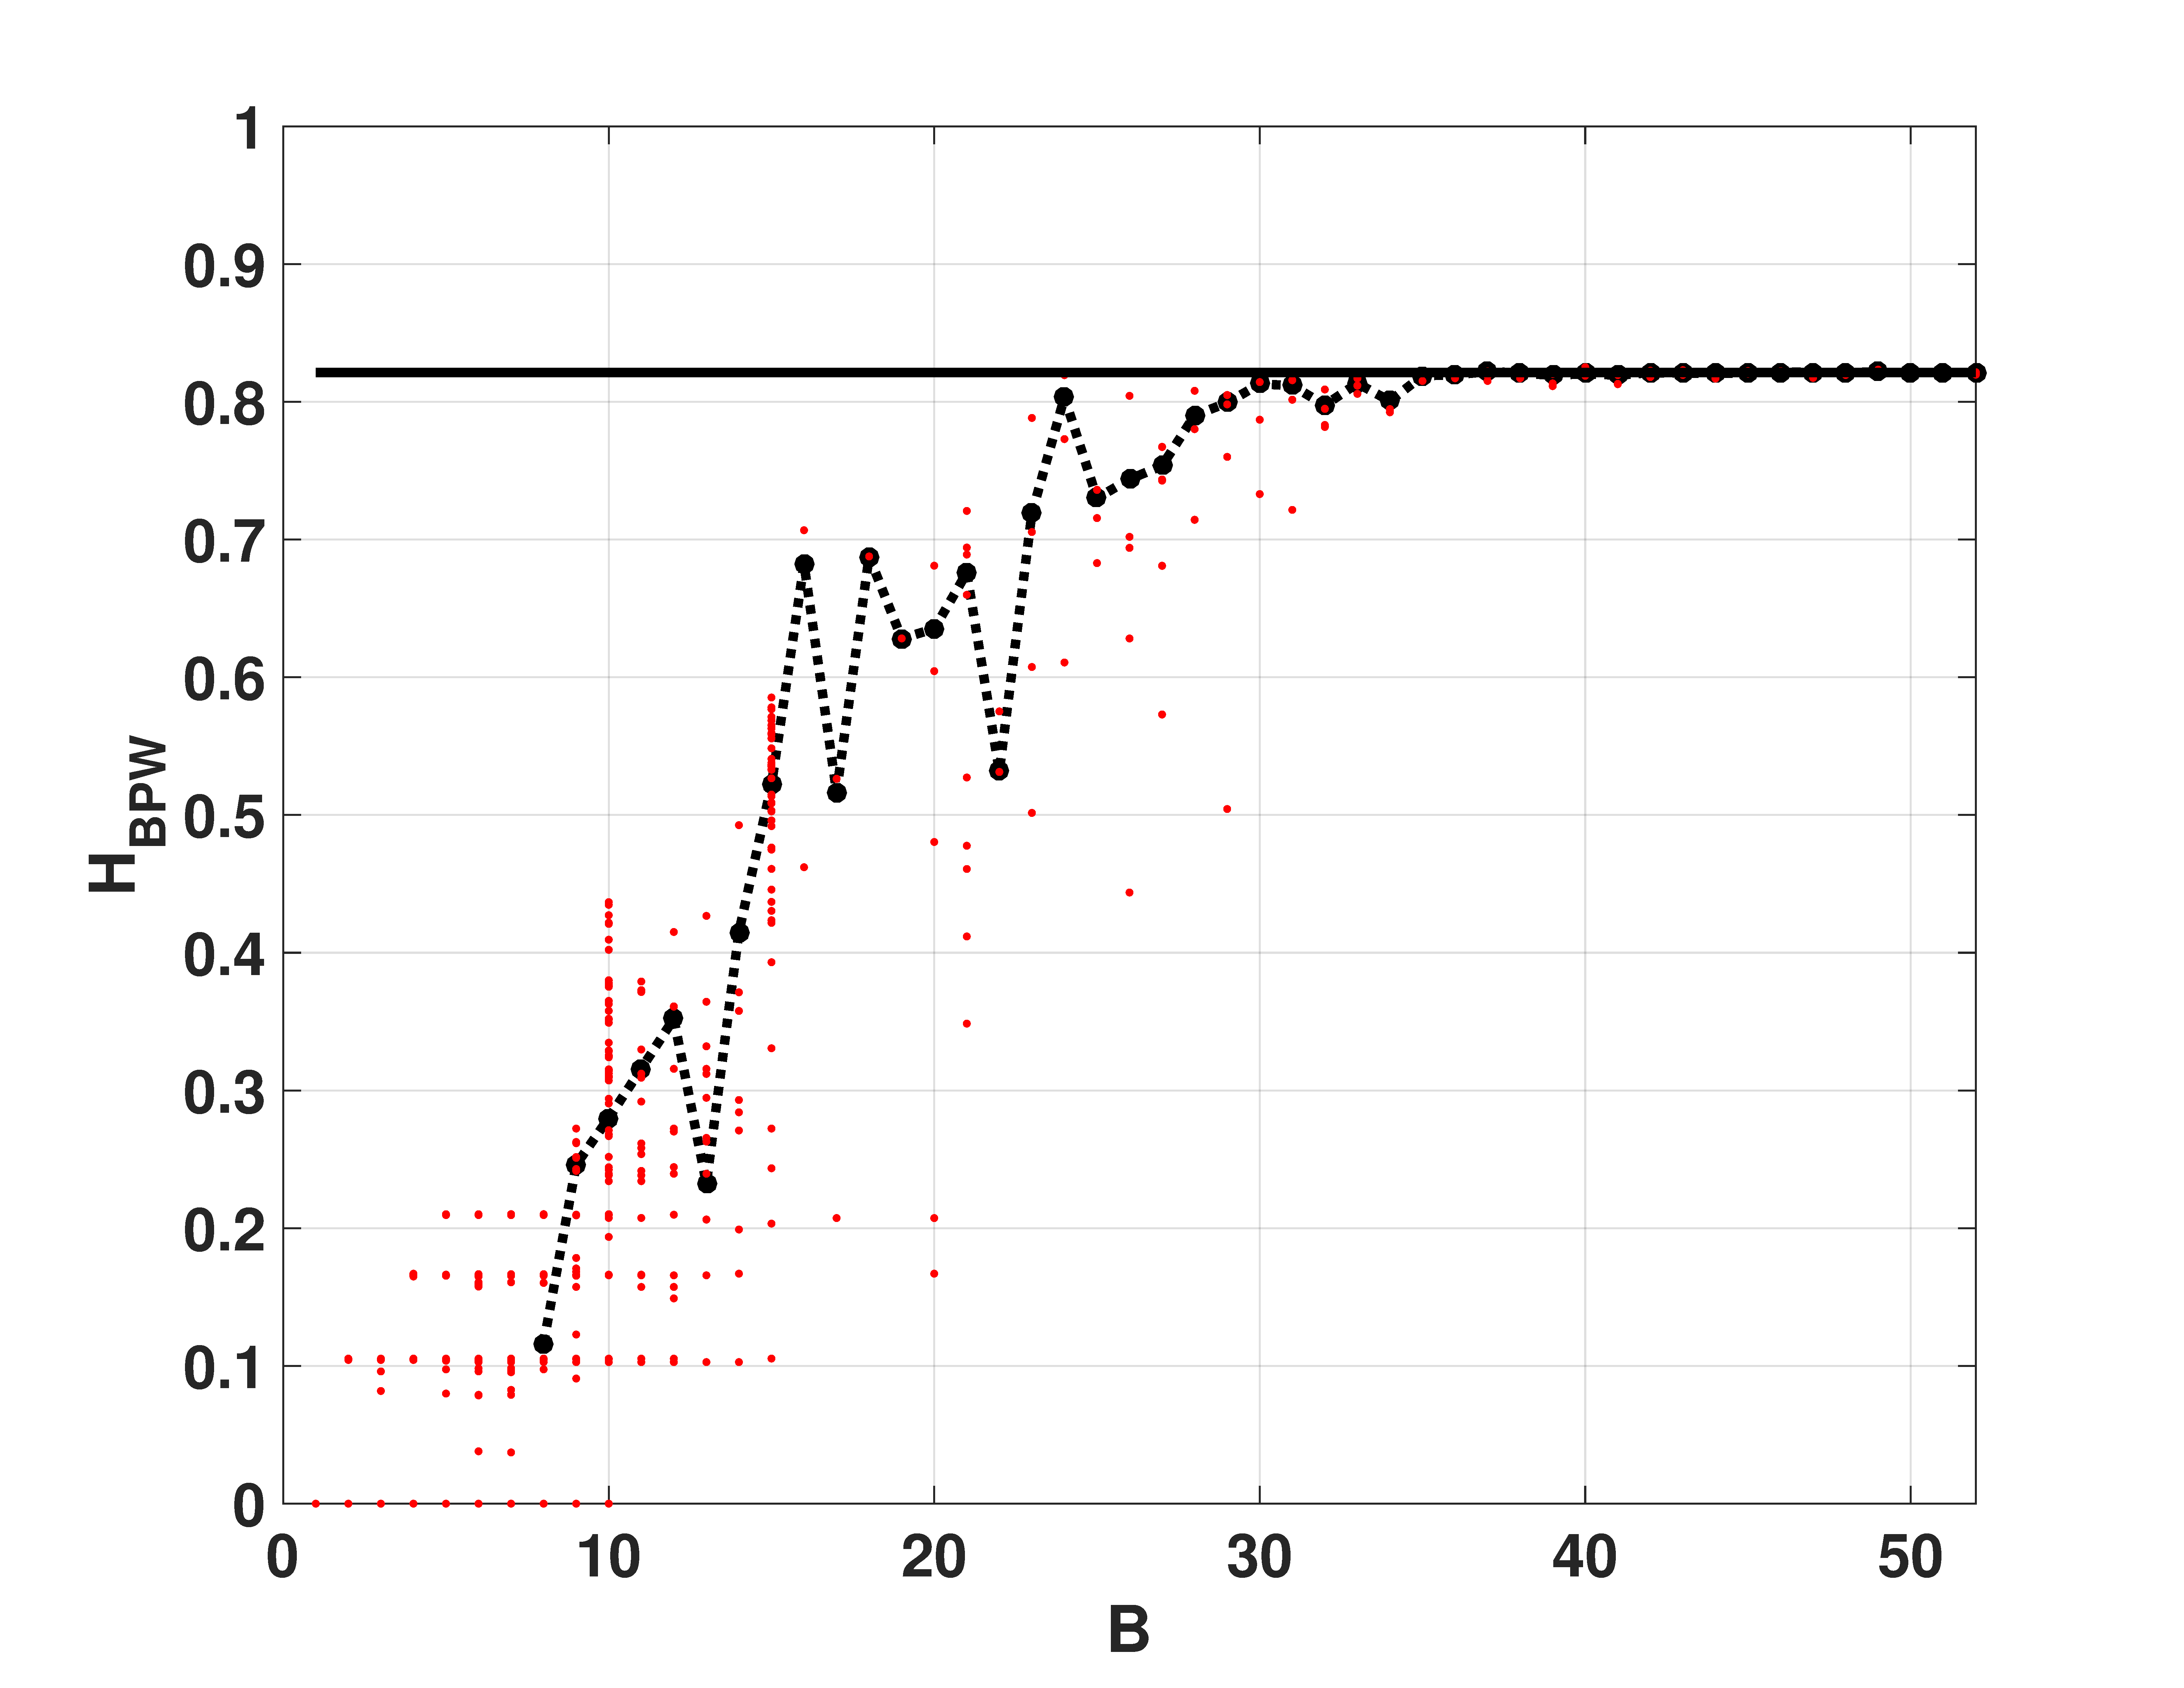
\includegraphics[width=\textwidth]{Hbpw_Even}
		\caption{$H_{BPW}$ vs. $B$}
		\label{fig:Hbpw_Even}
	\end{subfigure}
	\begin{subfigure}[b]{0.49\textwidth}
		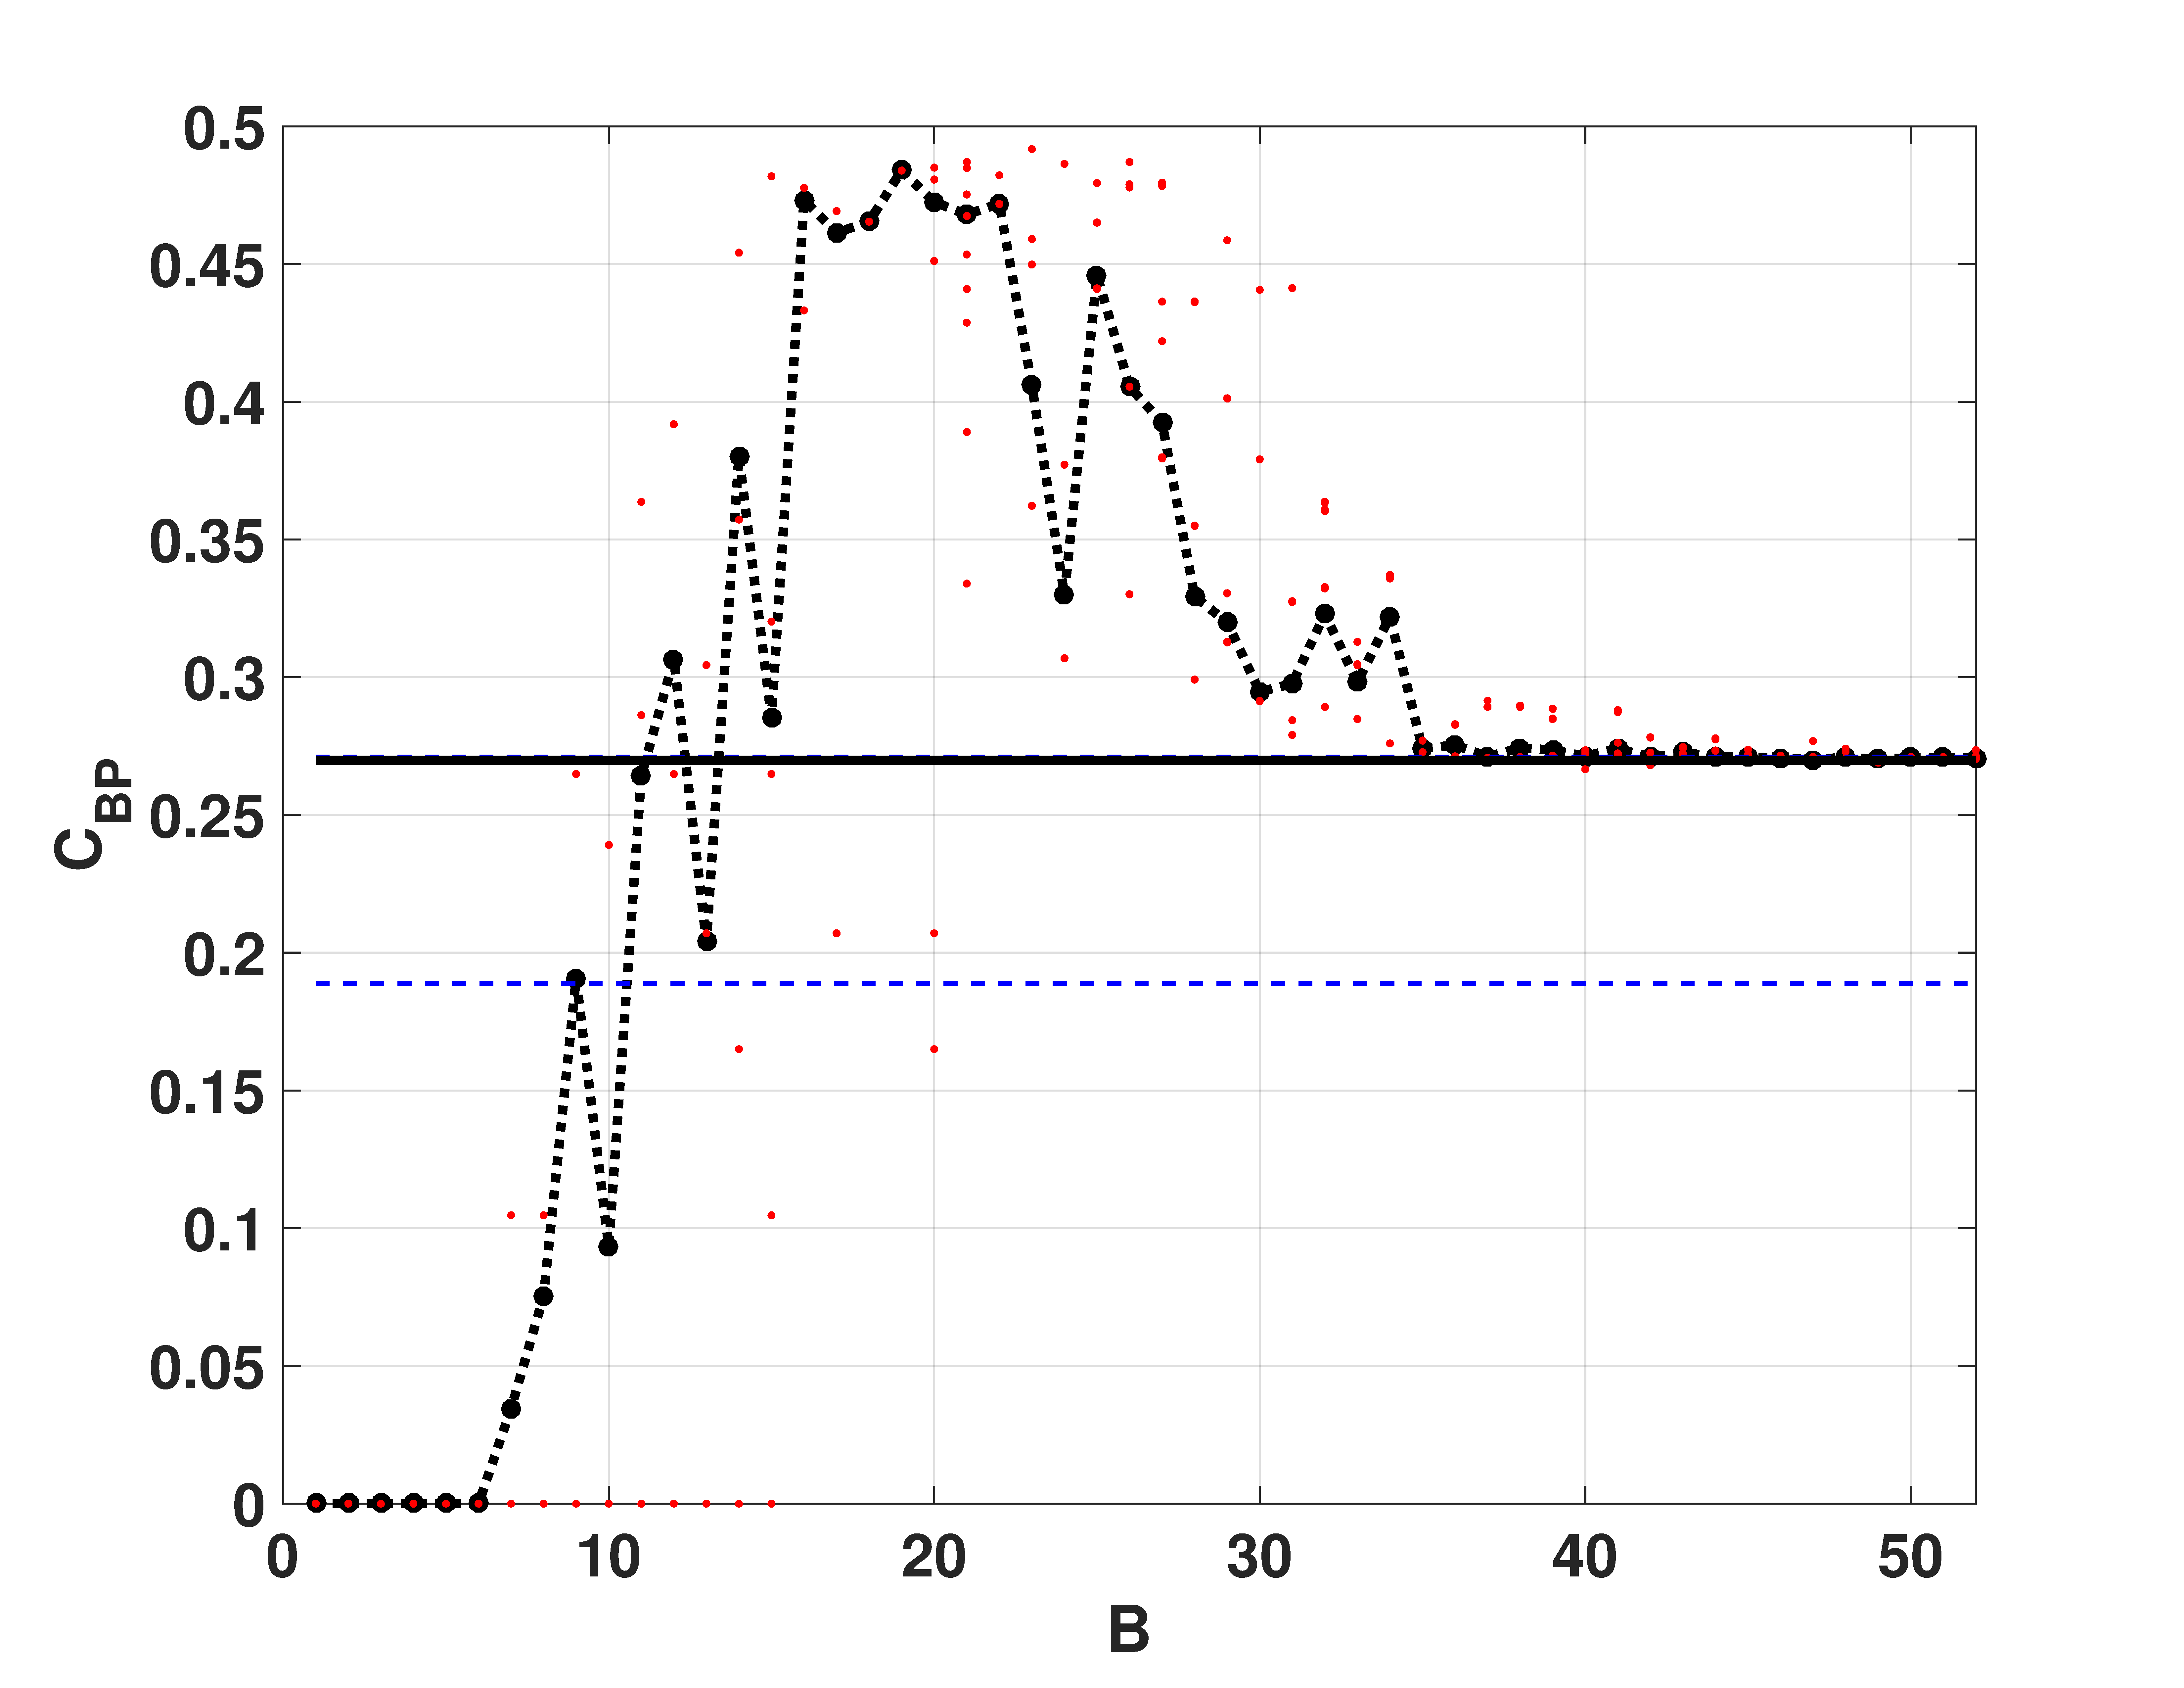
\includegraphics[width=\textwidth]{Cbp_Even}
		\caption{$C_{BP}$ vs. $B$}
		\label{fig:Cbp_Even}
	\end{subfigure}
	\begin{subfigure}[b]{0.49\textwidth}
		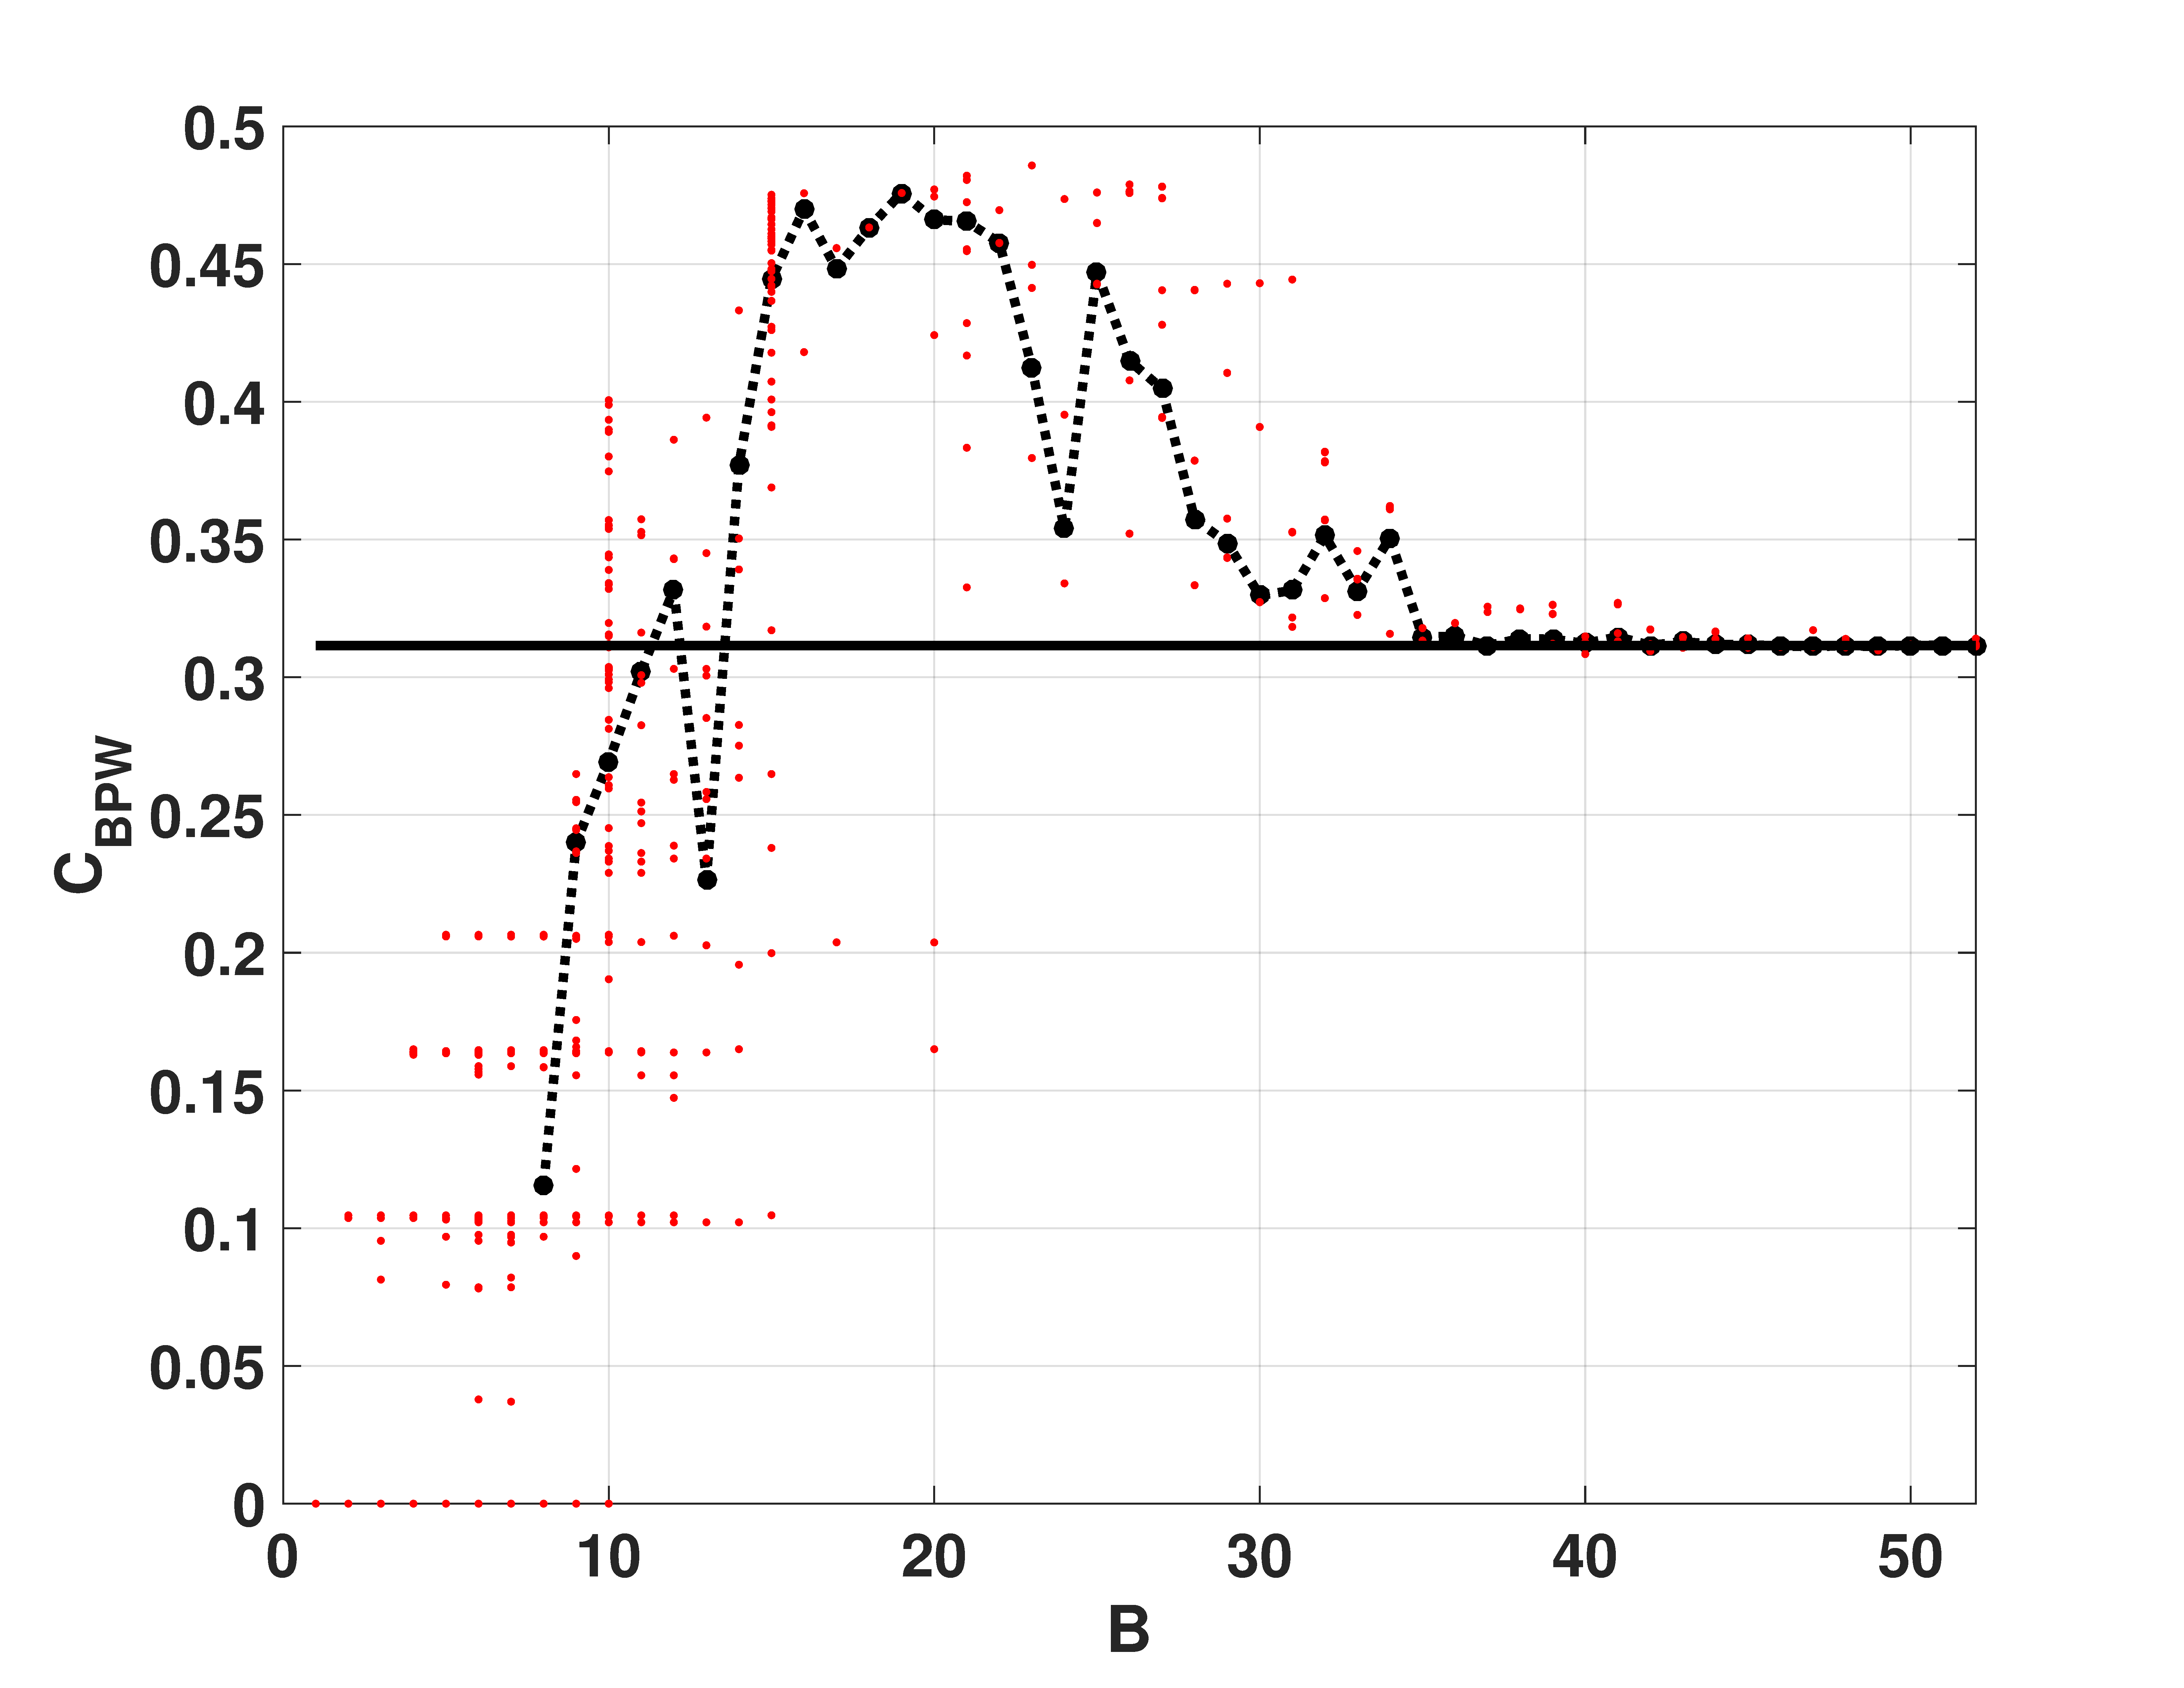
\includegraphics[width=\textwidth]{Cbpw_Even}
		\caption{$C_{BPW}$ vs. $B$}
		\label{fig:Cbpw_Even}
	\end{subfigure}
	\begin{subfigure}[b]{0.49\textwidth}
		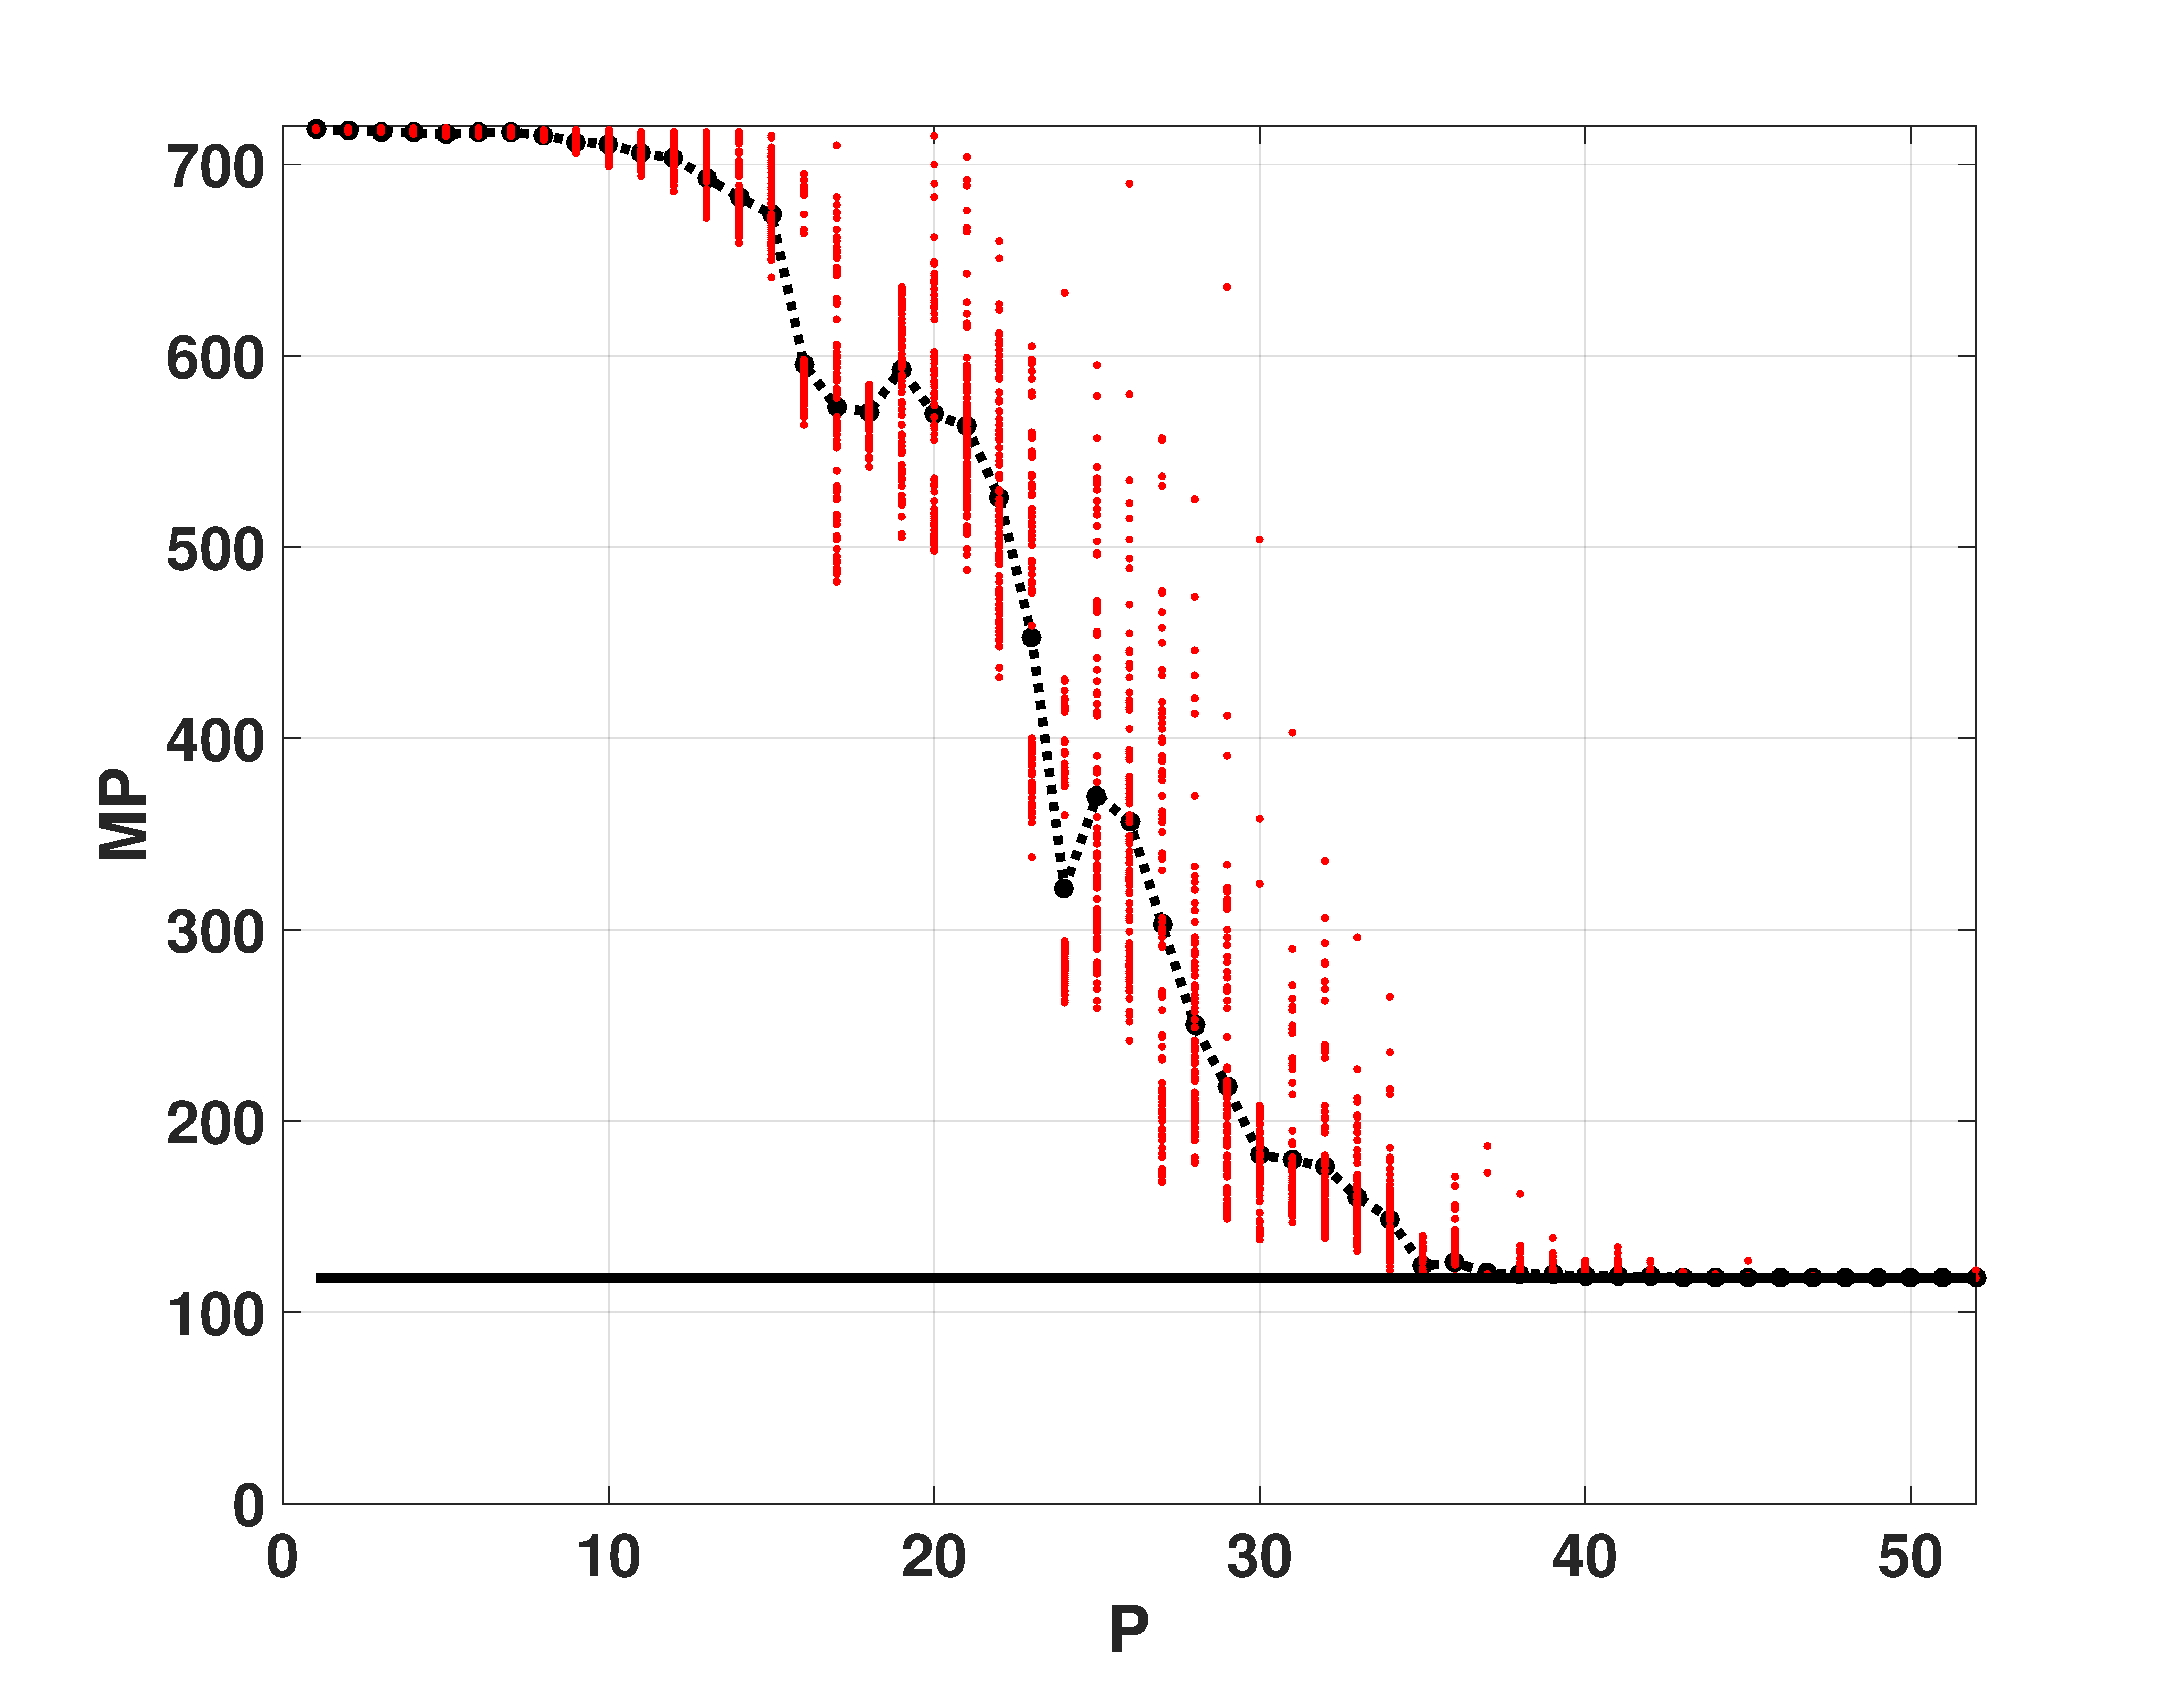
\includegraphics[width=\textwidth]{MP_Even}
		\caption{MP vs. $B$}
		\label{fig:MP_Even}
	\end{subfigure}
	\caption{Statistical properties of EVEN map.}
	\label{fig:EVEN_QuantiB}
\end{figure}
%
\begin{figure}[H]
	\centering
	\begin{subfigure}[b]{0.49\textwidth}
		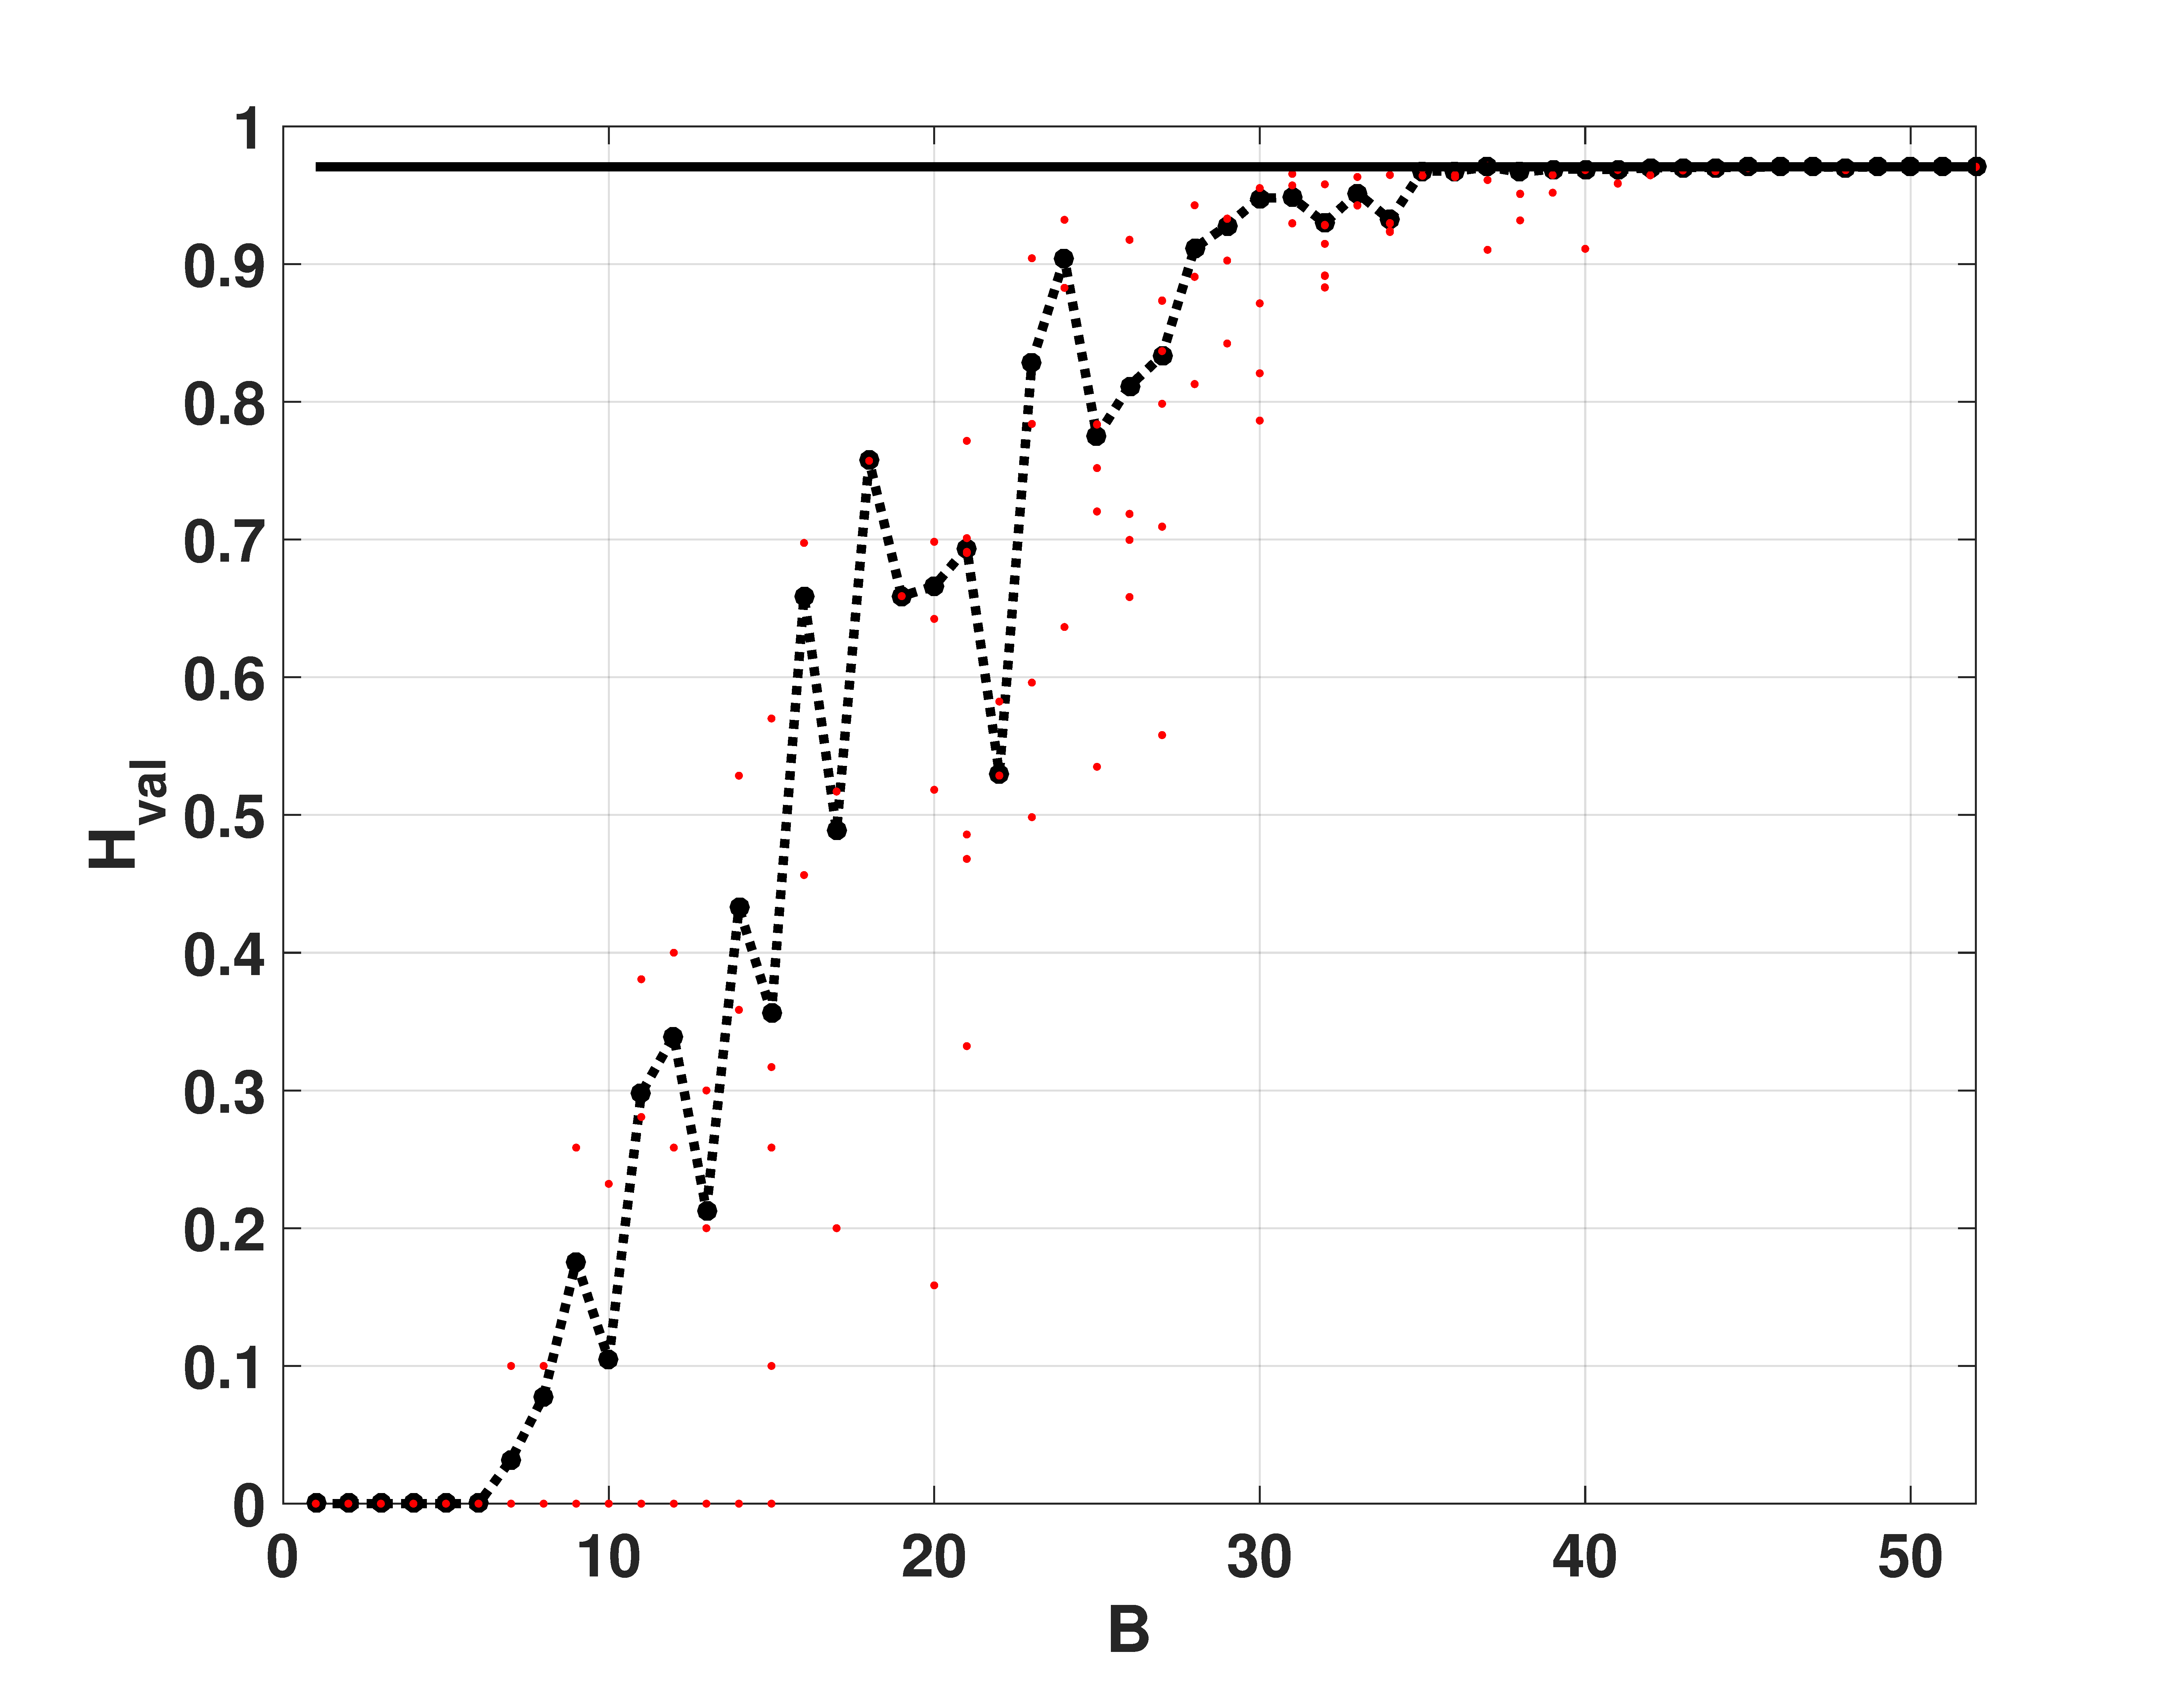
\includegraphics[width=\textwidth]{Hval_Odd}
		\caption{$H_{hist}$ vs. $B$}
		\label{fig:Hval_Odd}
	\end{subfigure}
	\begin{subfigure}[b]{0.49\textwidth}
		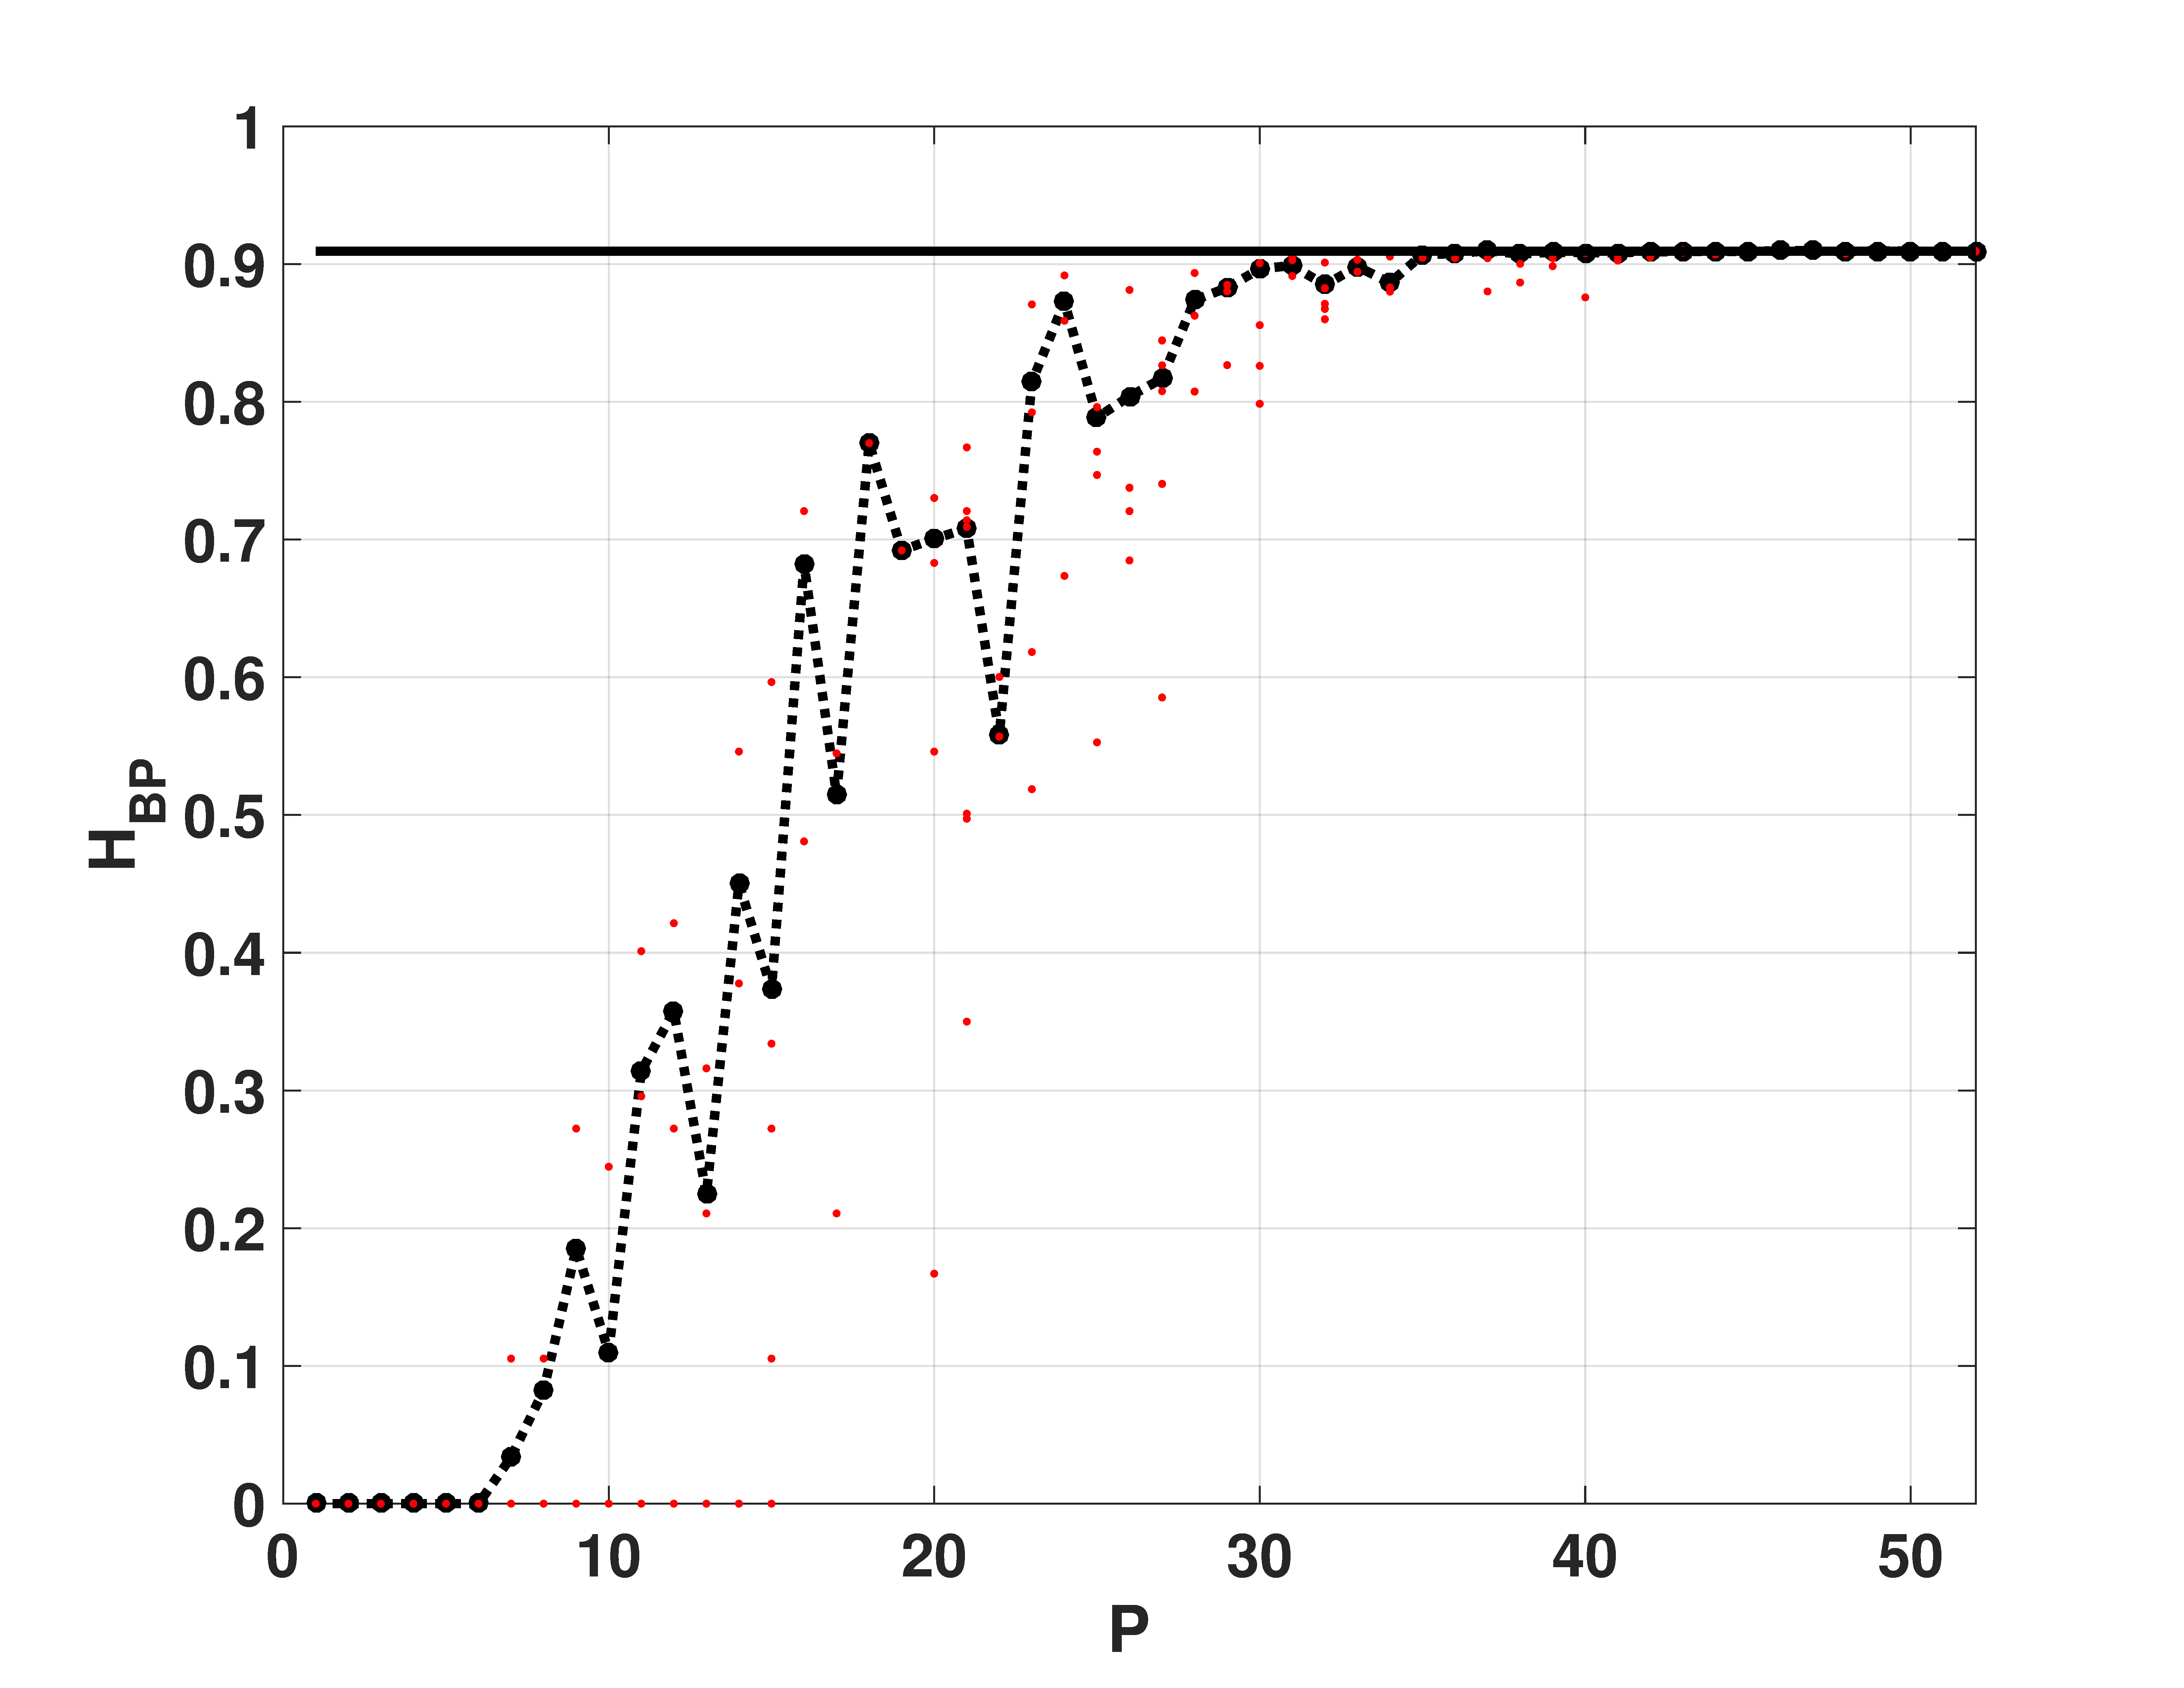
\includegraphics[width=\textwidth]{Hbp_Odd}
		\caption{$H_{BP}$ vs. $B$}
		\label{fig:Hbp_Odd}
	\end{subfigure}
	\begin{subfigure}[b]{0.49\textwidth}
		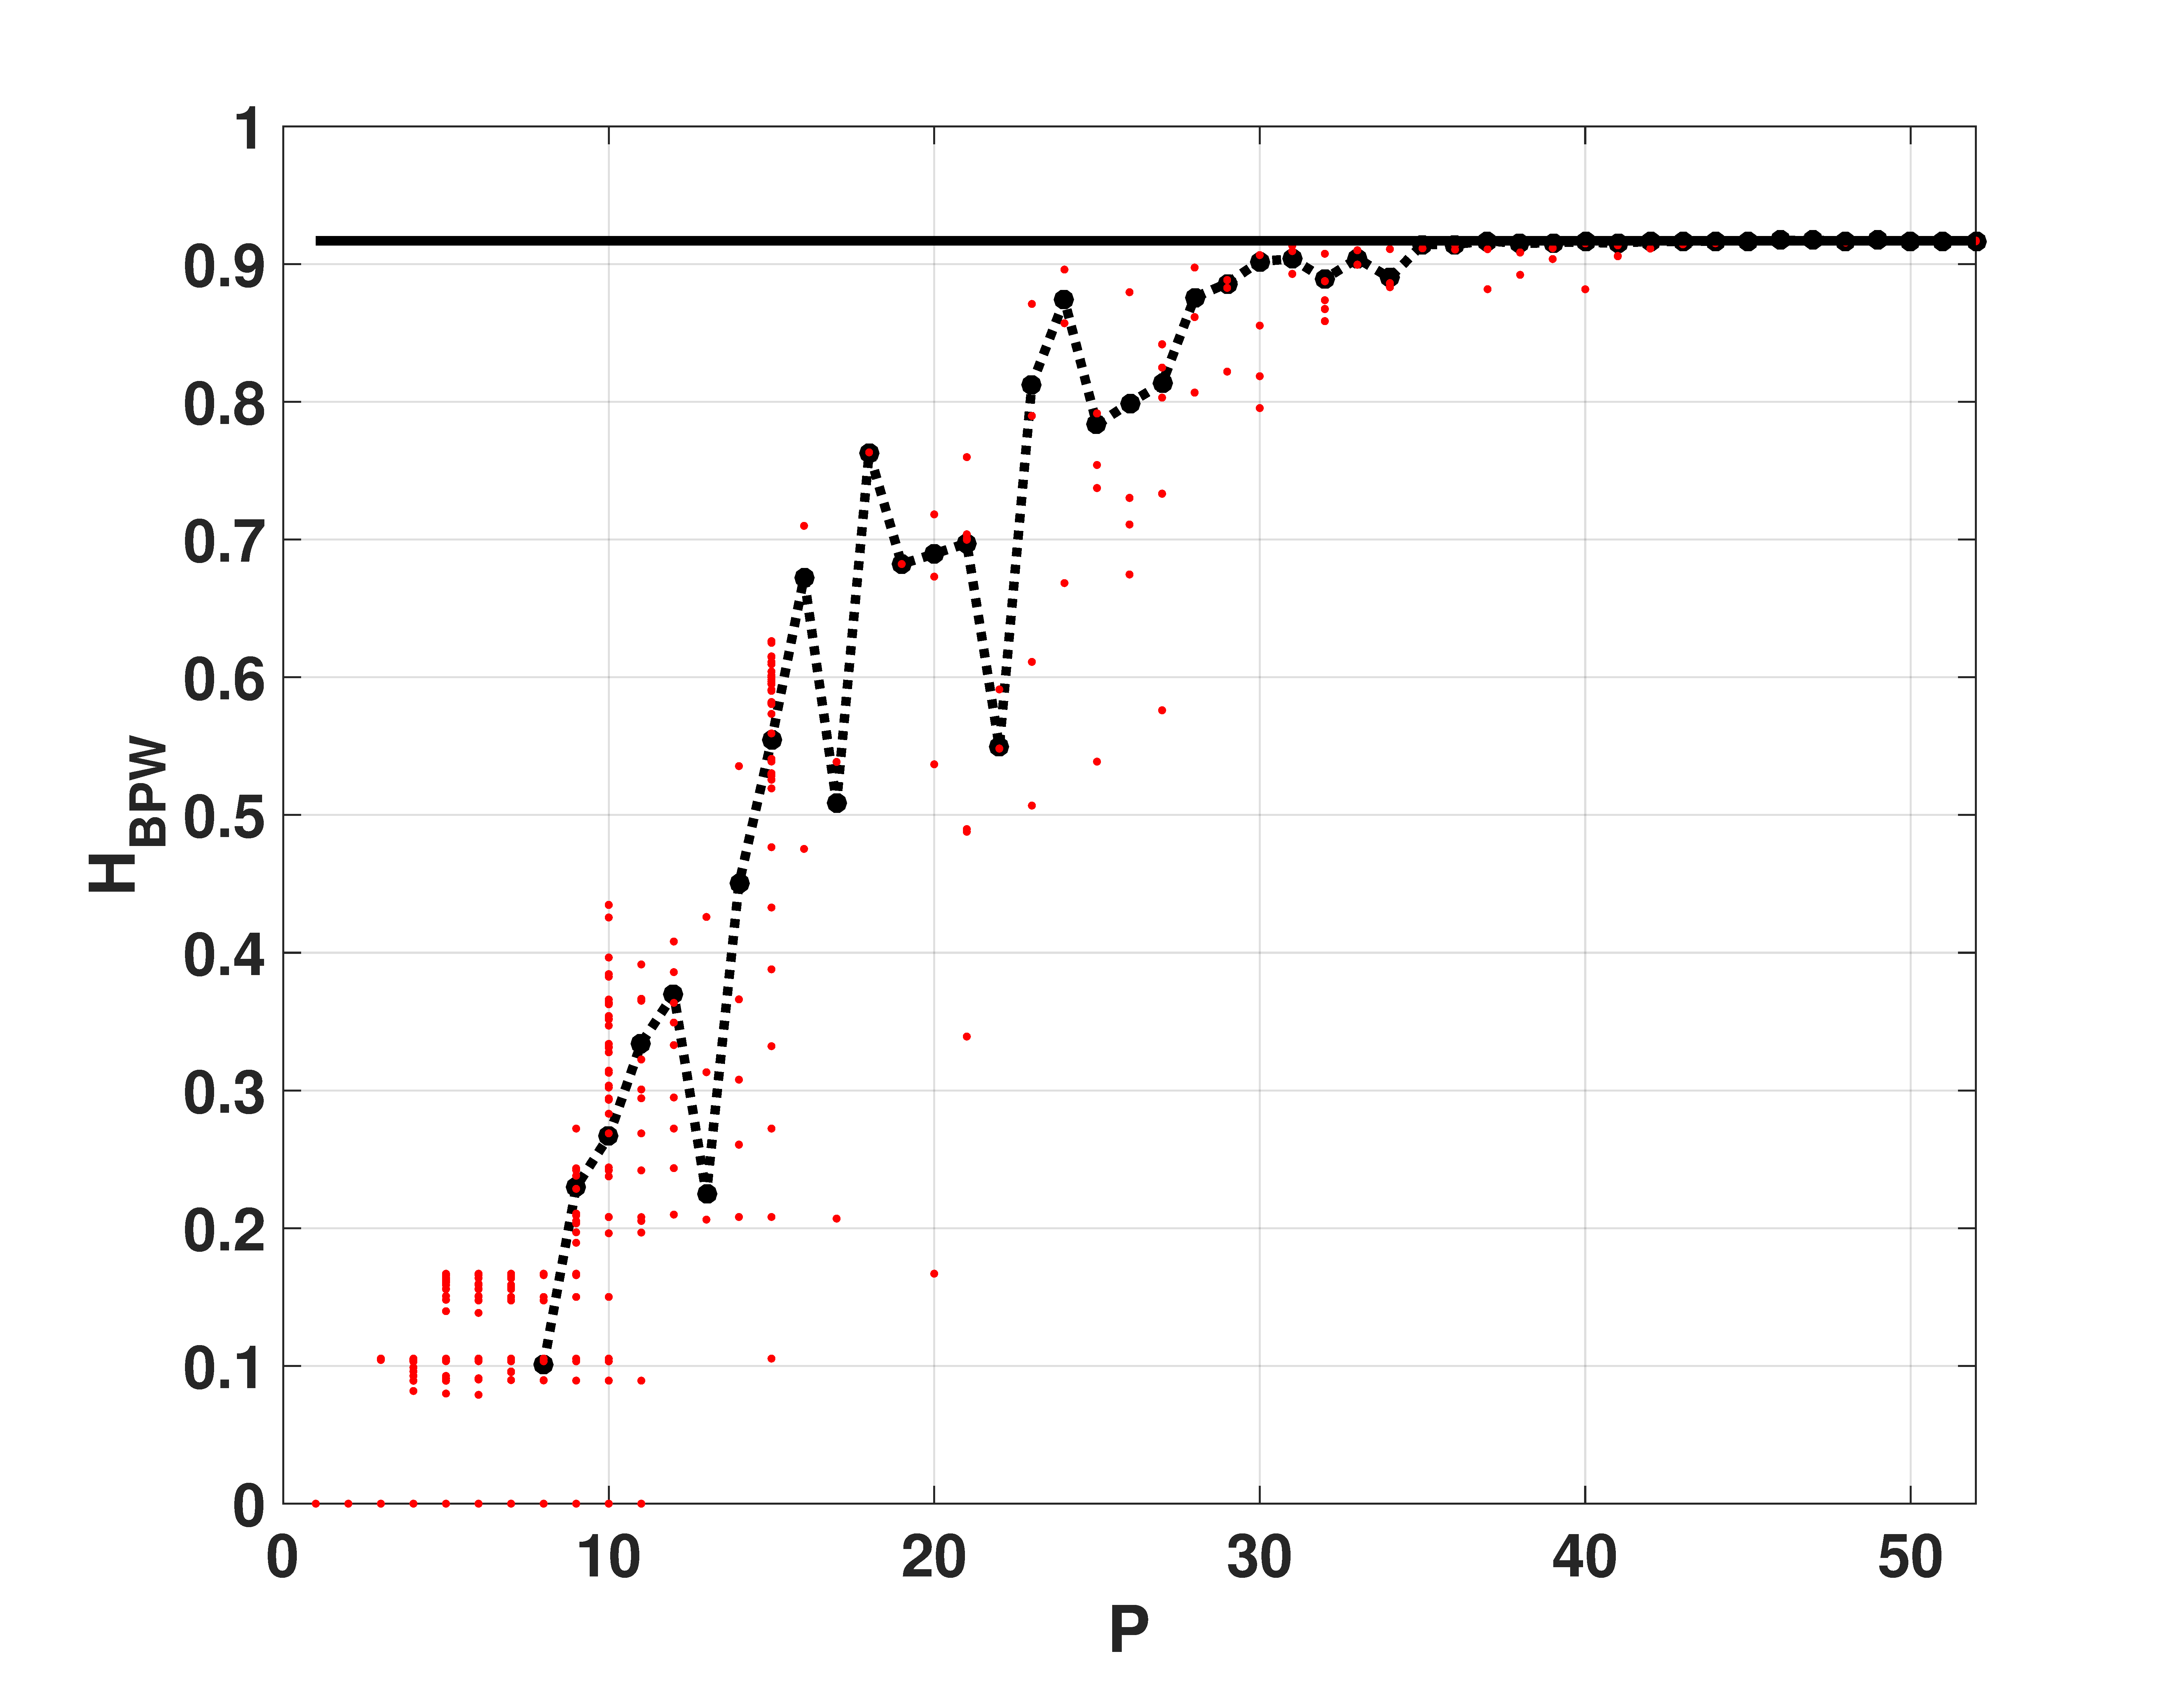
\includegraphics[width=\textwidth]{Hbpw_Odd}
		\caption{$H_{BPW}$ vs. $B$}
		\label{fig:Hbpw_Odd}
	\end{subfigure}
	\begin{subfigure}[b]{0.49\textwidth}
		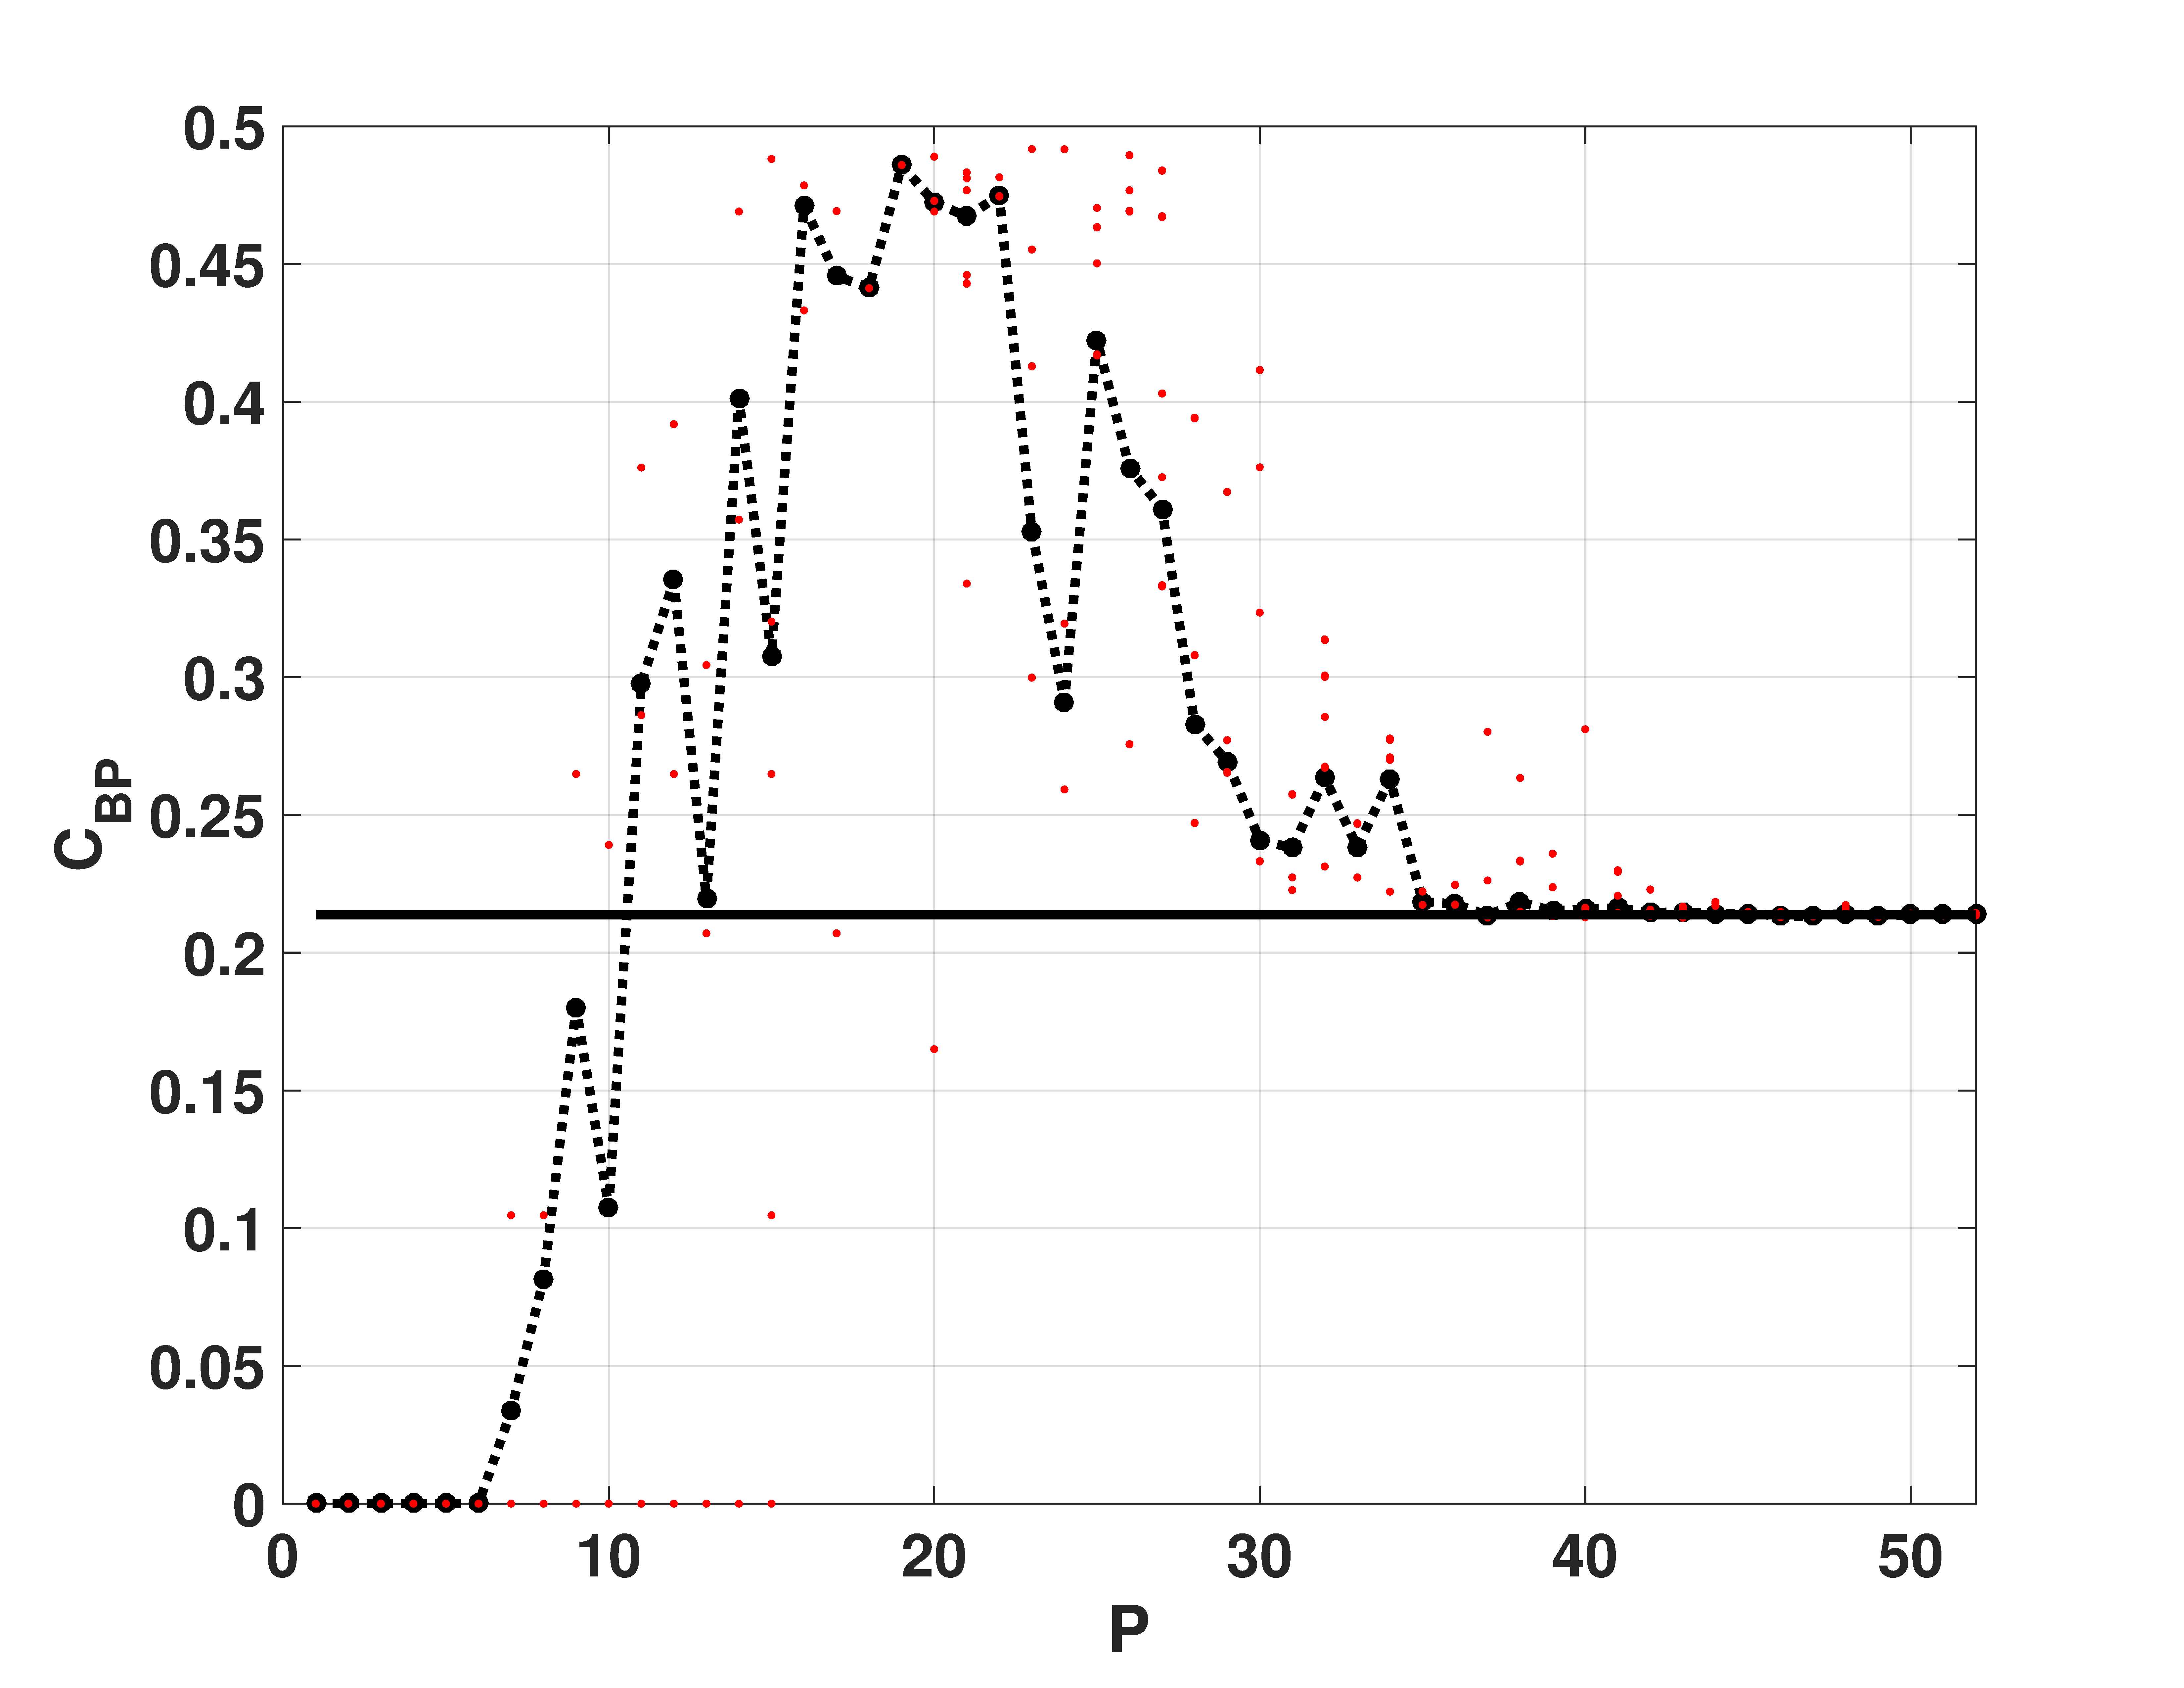
\includegraphics[width=\textwidth]{Cbp_Odd}
		\caption{$C_{BP}$ vs. $B$}
		\label{fig:Cbp_Odd}
	\end{subfigure}
	\begin{subfigure}[b]{0.49\textwidth}
		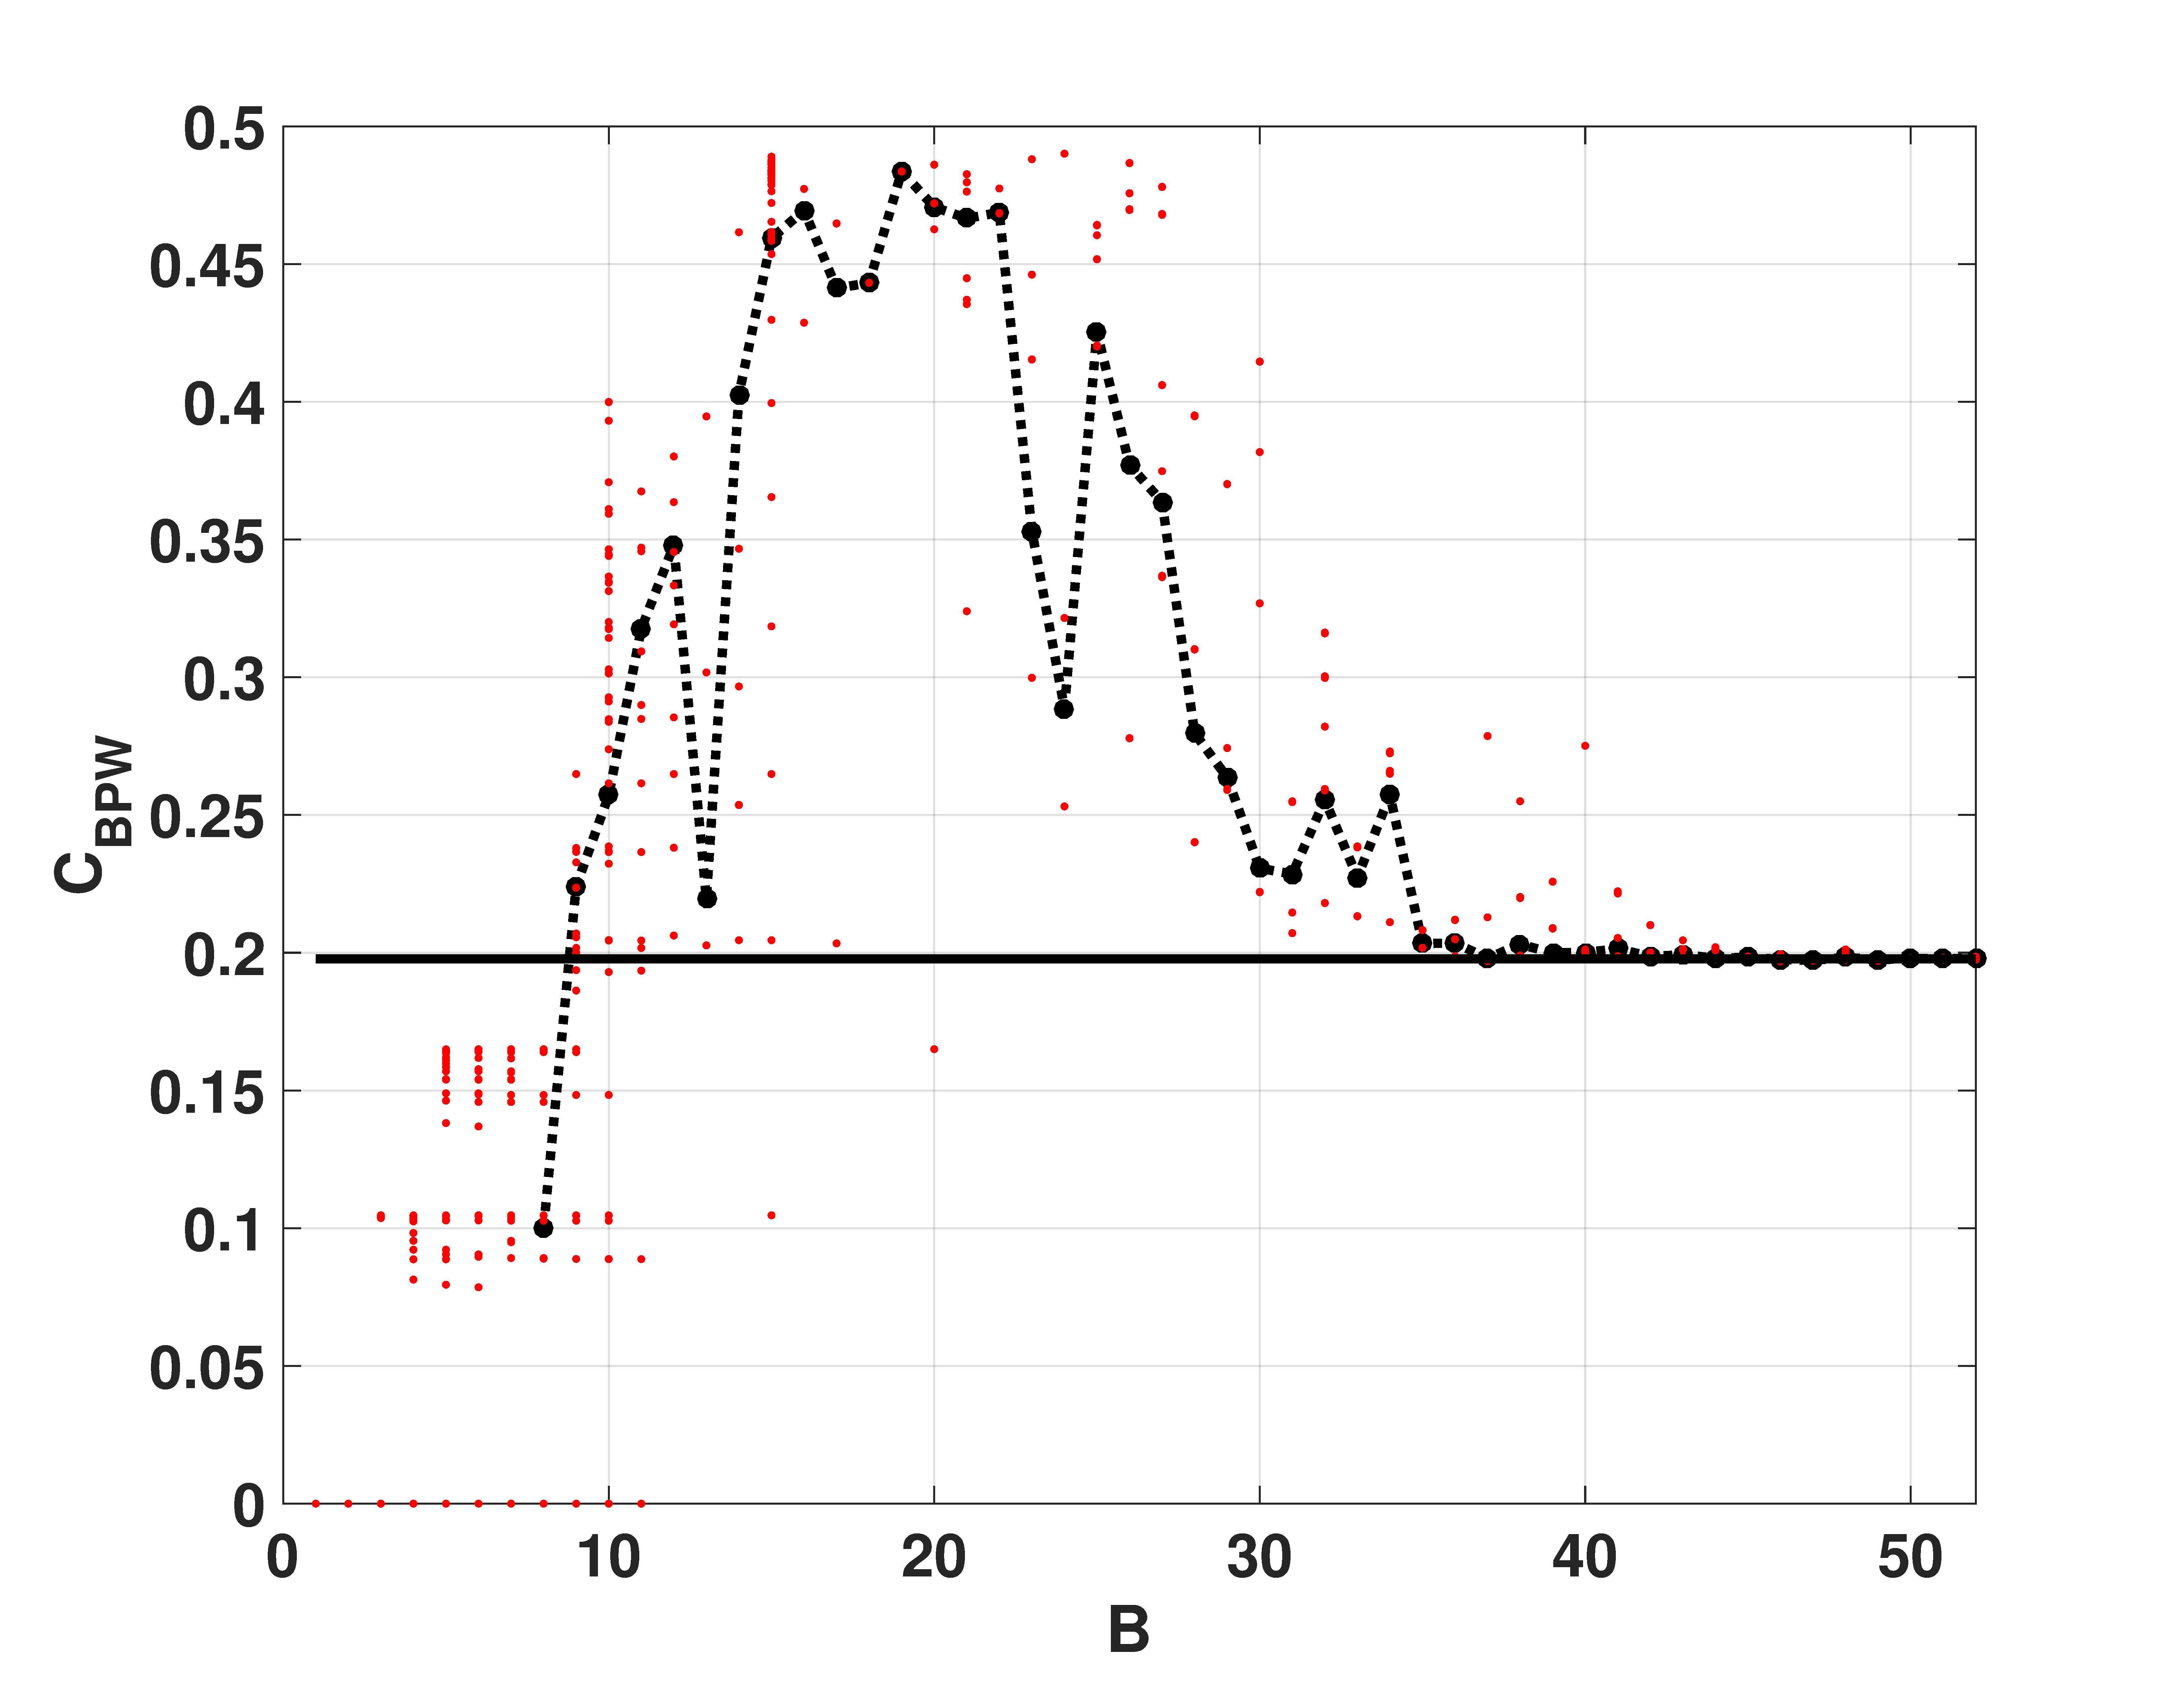
\includegraphics[width=\textwidth]{Cbpw_Odd}
		\caption{$C_{BPW}$ vs. $B$}
		\label{fig:Cbpw_Odd}
	\end{subfigure}
	\begin{subfigure}[b]{0.49\textwidth}
		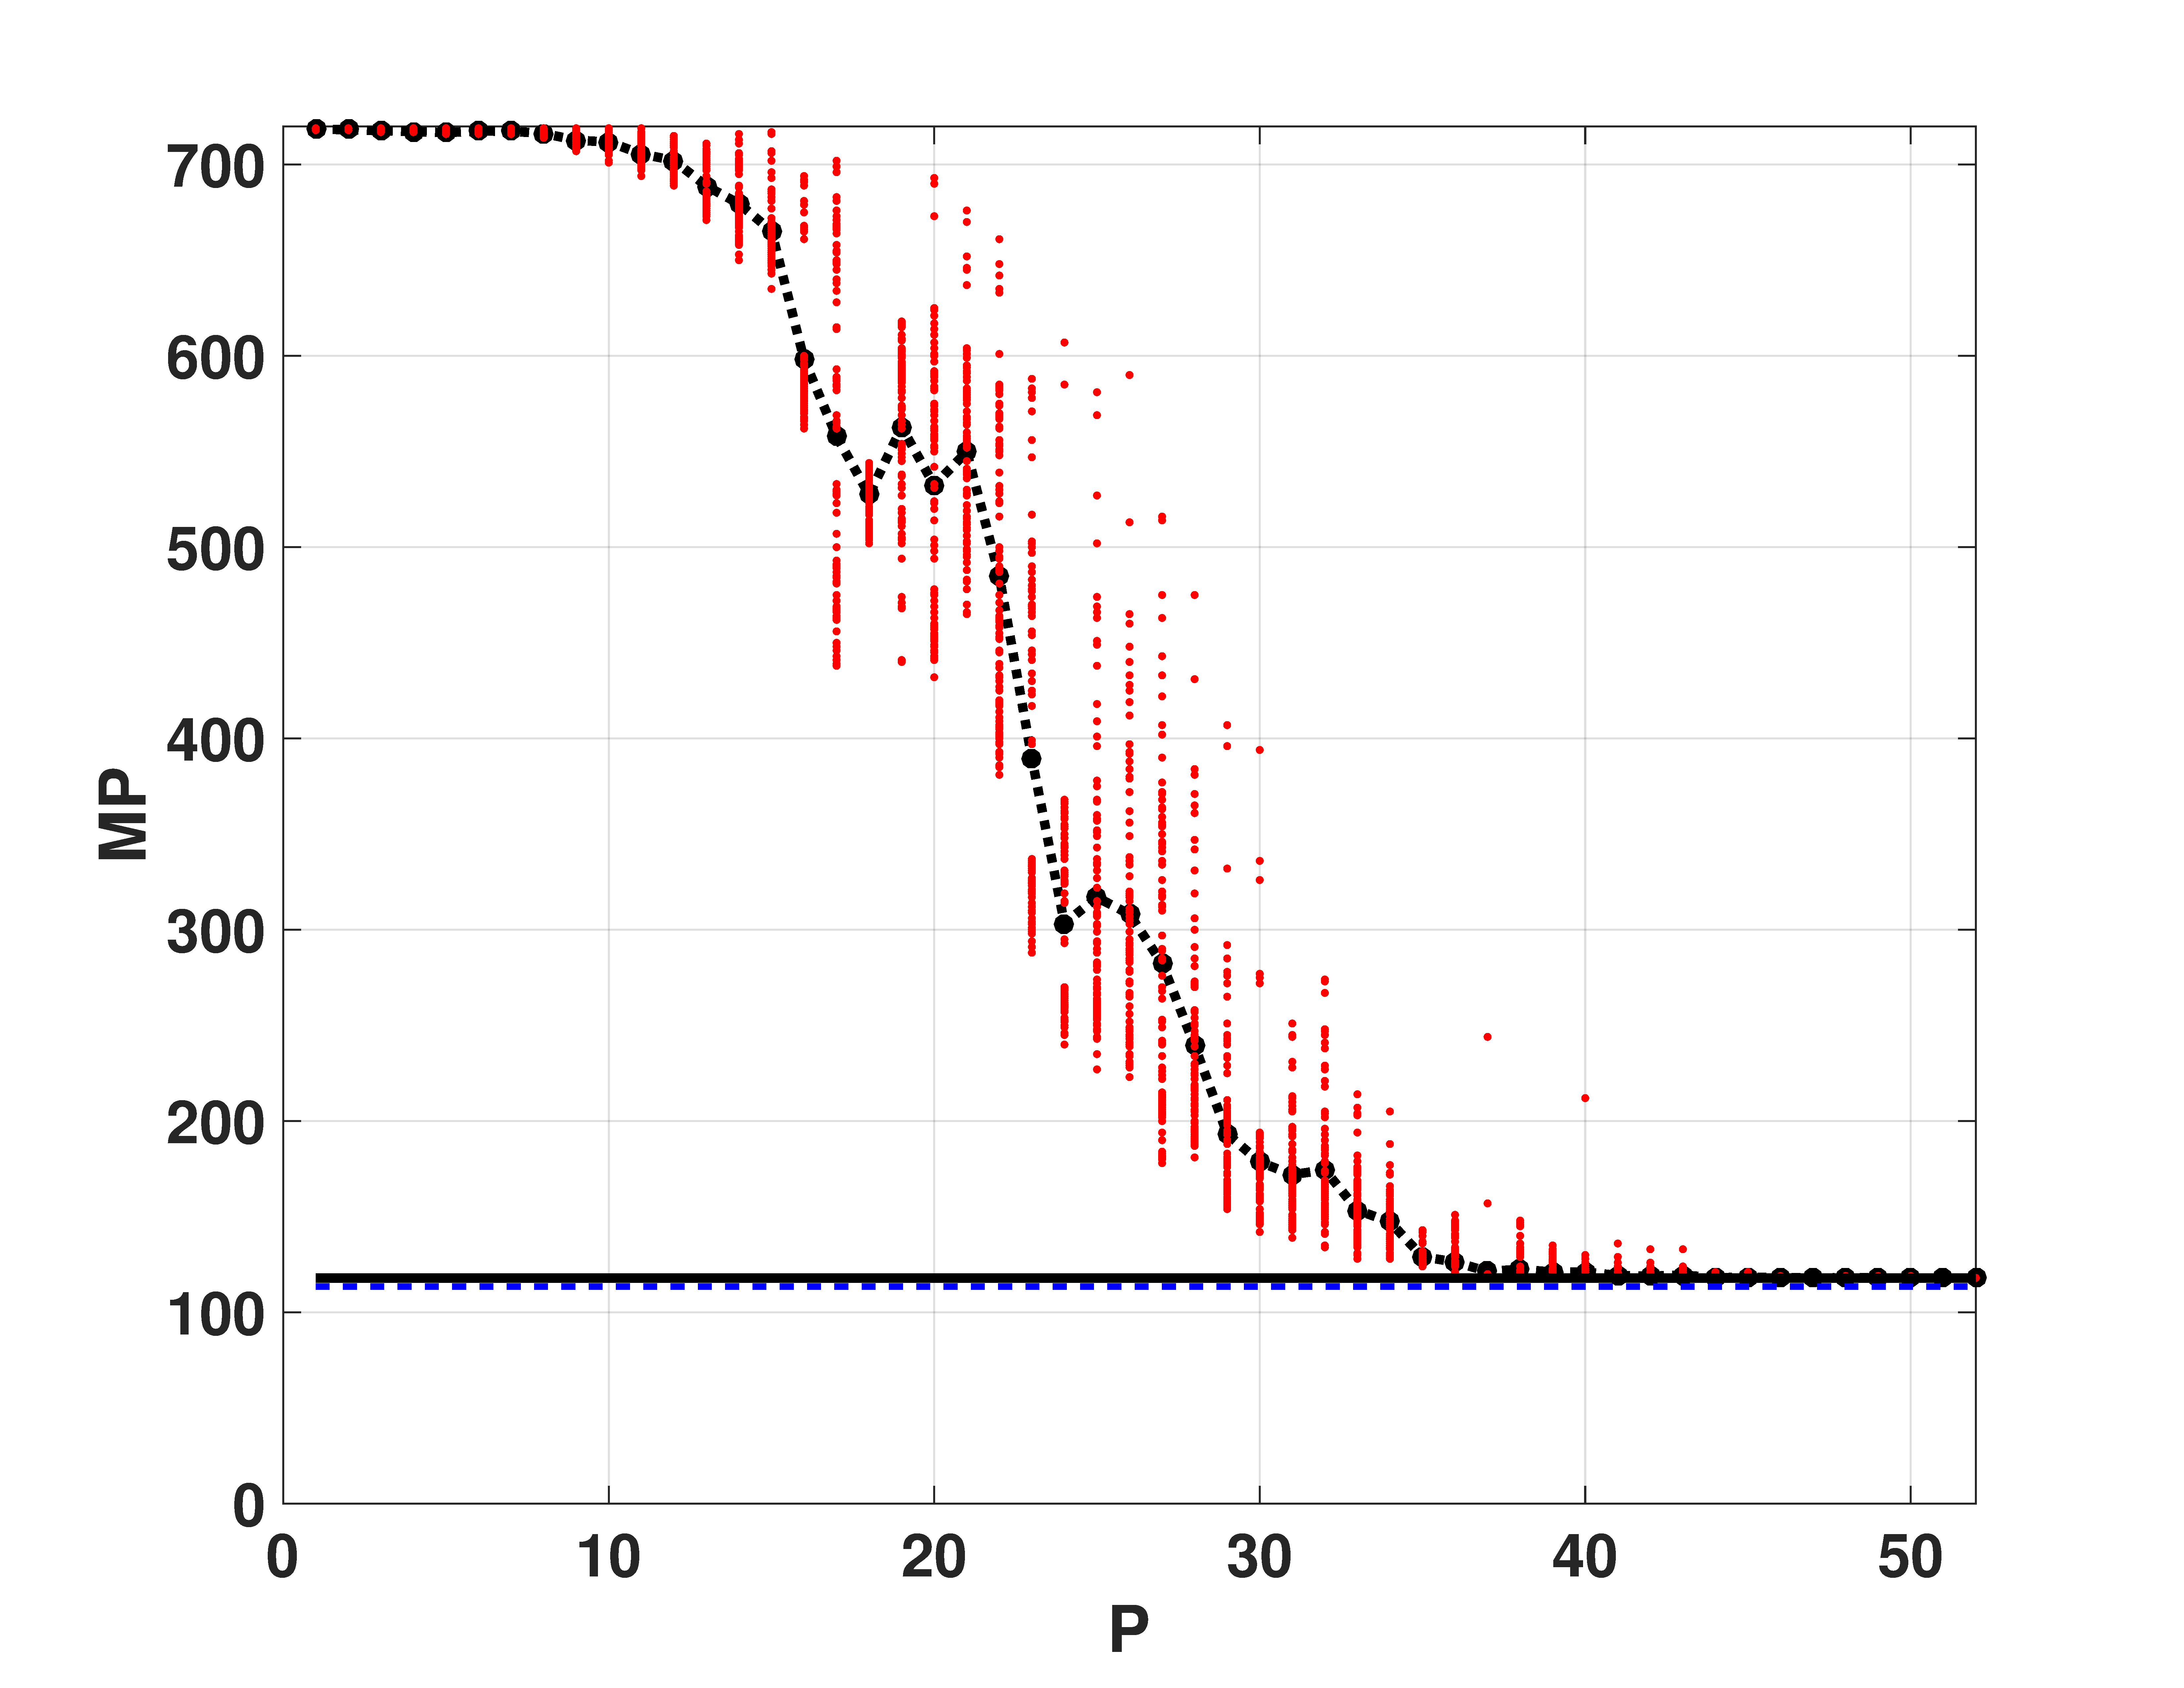
\includegraphics[width=\textwidth]{MP_Odd}
		\caption{MP vs. $B$}
		\label{fig:MP_Odd}
	\end{subfigure}
	\caption{Statistical properties of ODD map.}
	\label{fig:ODD_QuantiB}
\end{figure}

The enhancement showed in Figures \ref{fig:EVEN_QuantiB} and \ref{fig:ODD_QuantiB} is reflected in the position of asymptotic point in the planes \ref{fig:EVEN_HH}, and \ref{fig:ODD_HH}.
In both cases this position is closest to the ideal point $(H_{hist}, H_{BP})=(1, 1)$, because the resulting vectors present better mixing.
%
\begin{figure}[H]
	\centering
	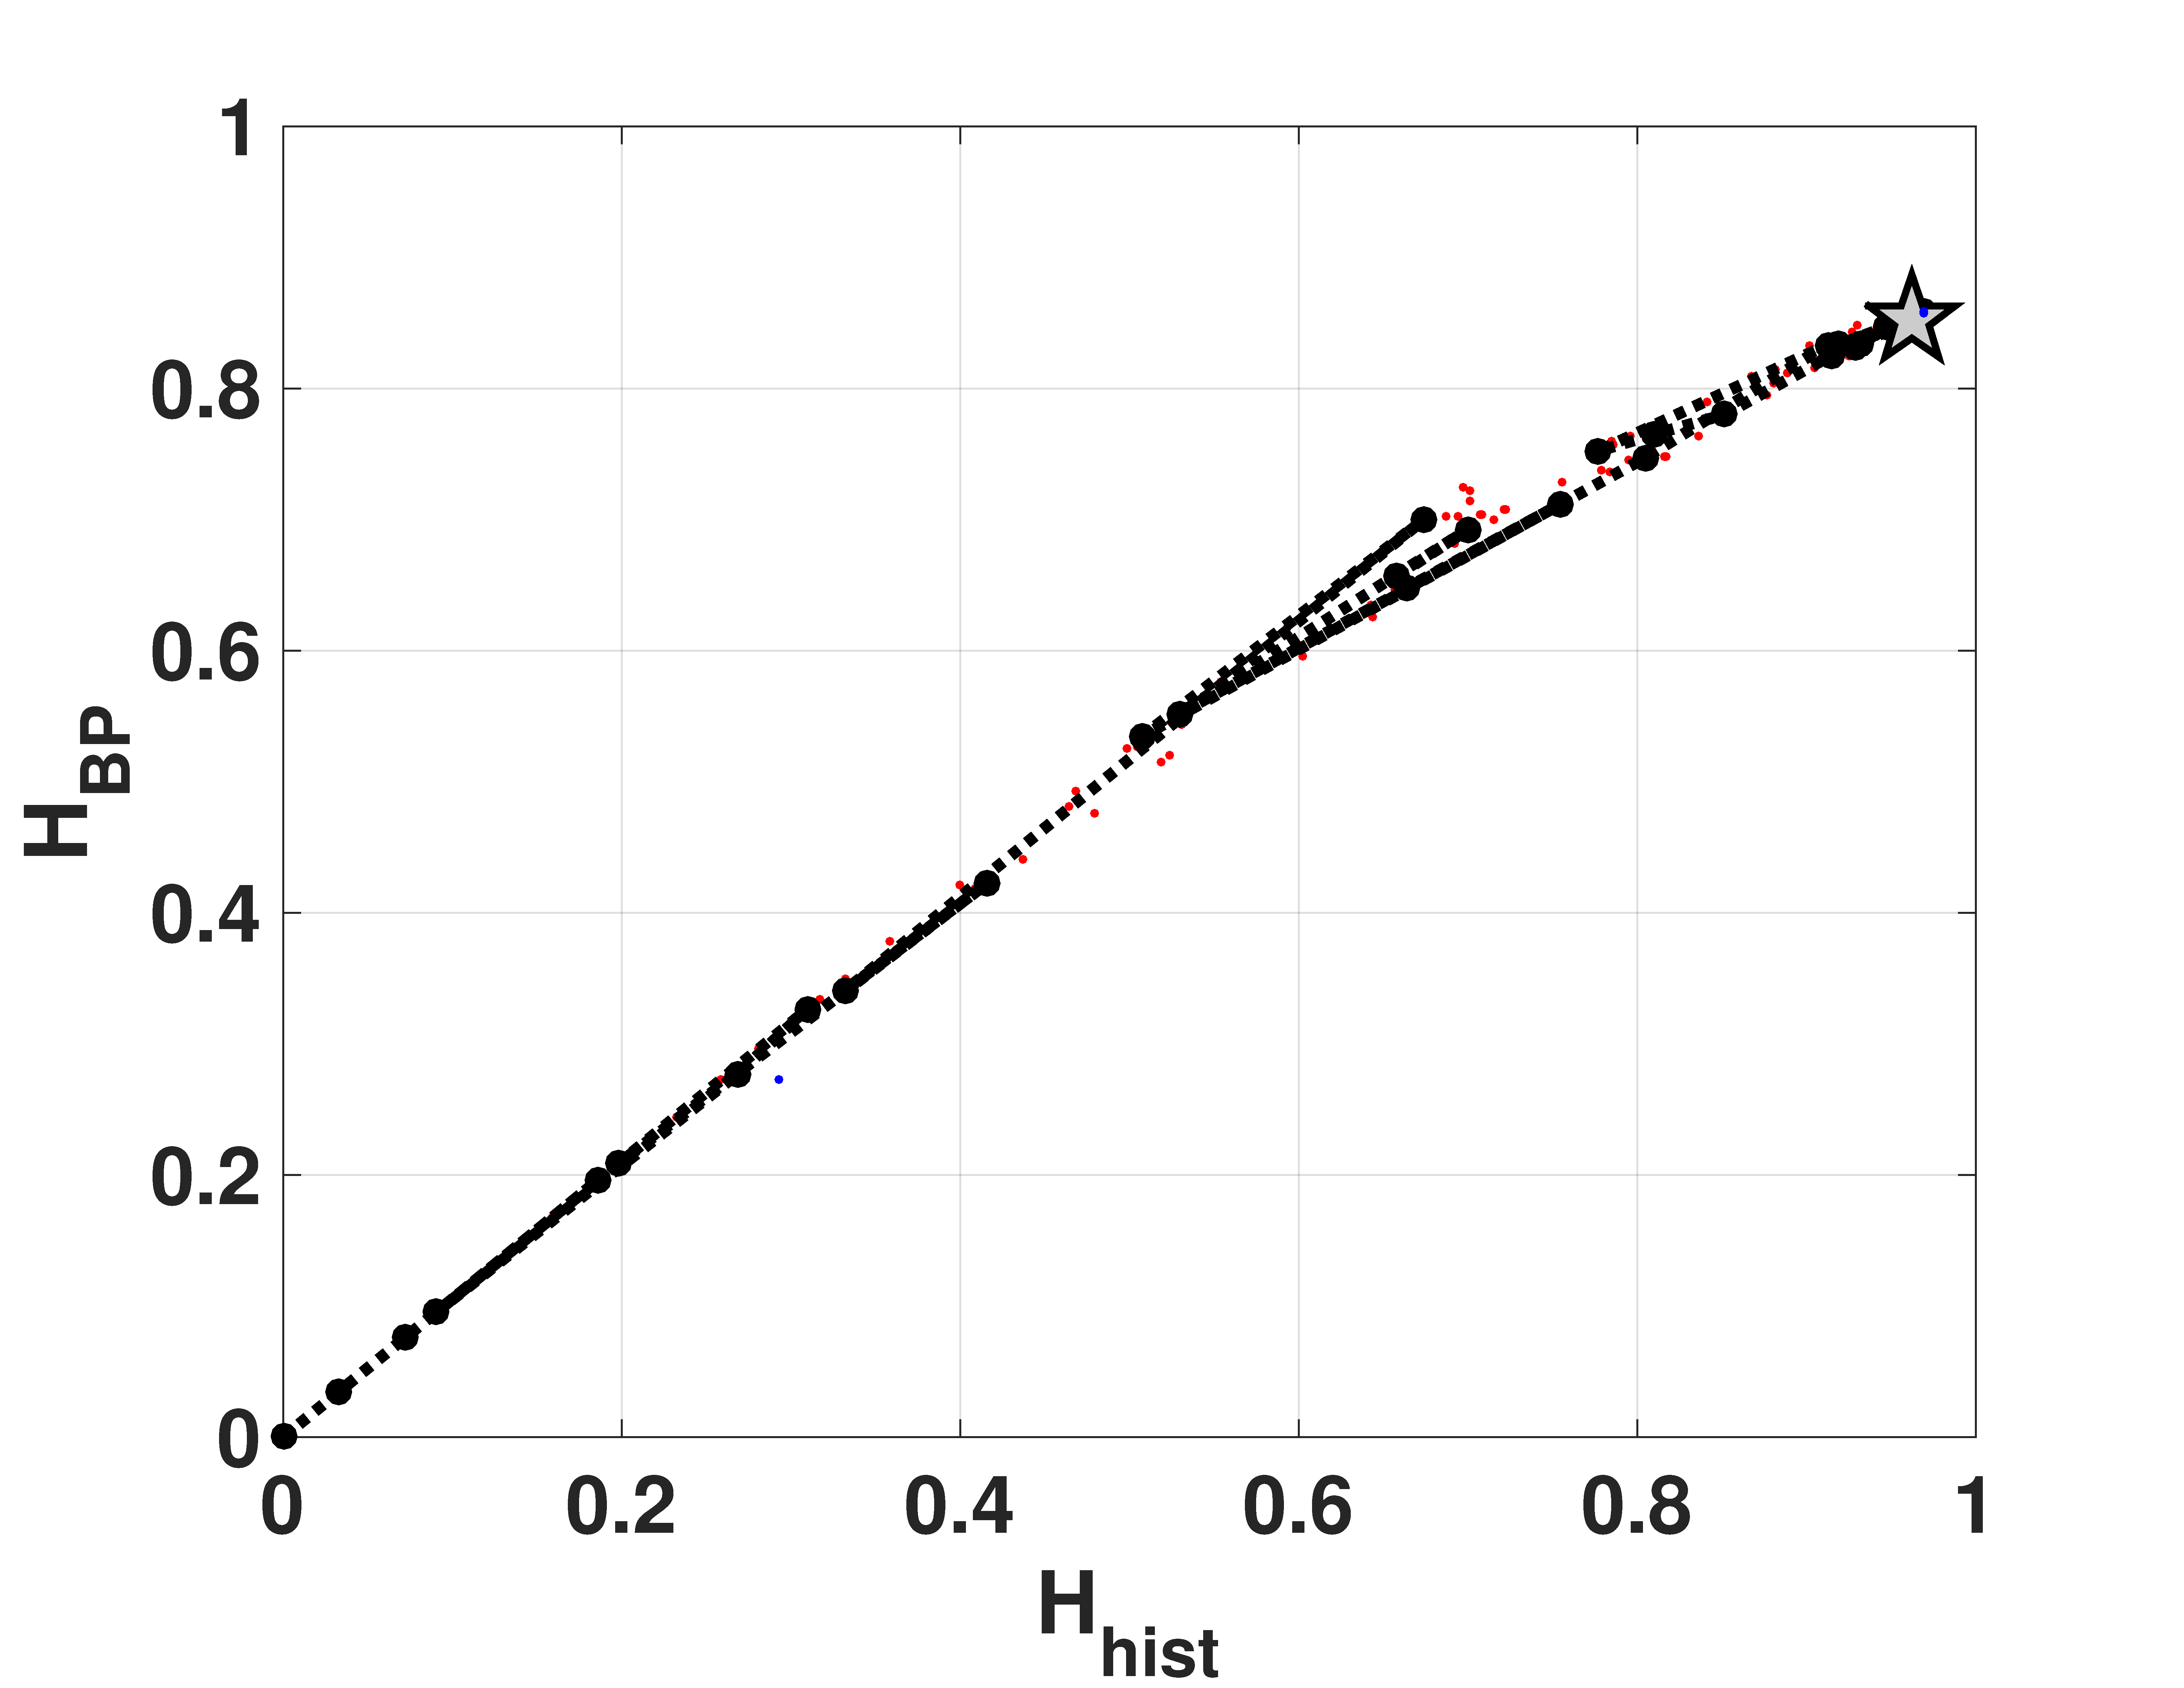
\includegraphics[width=.49\textwidth]{HbpHval_Even}
	\caption{Evolution of statistical properties in double entropy plane for EVEN map $H_{hist} \times H_{BP}$.}
	\label{fig:EVEN_HH}
\end{figure}
%
\begin{figure}[H]
	\centering
	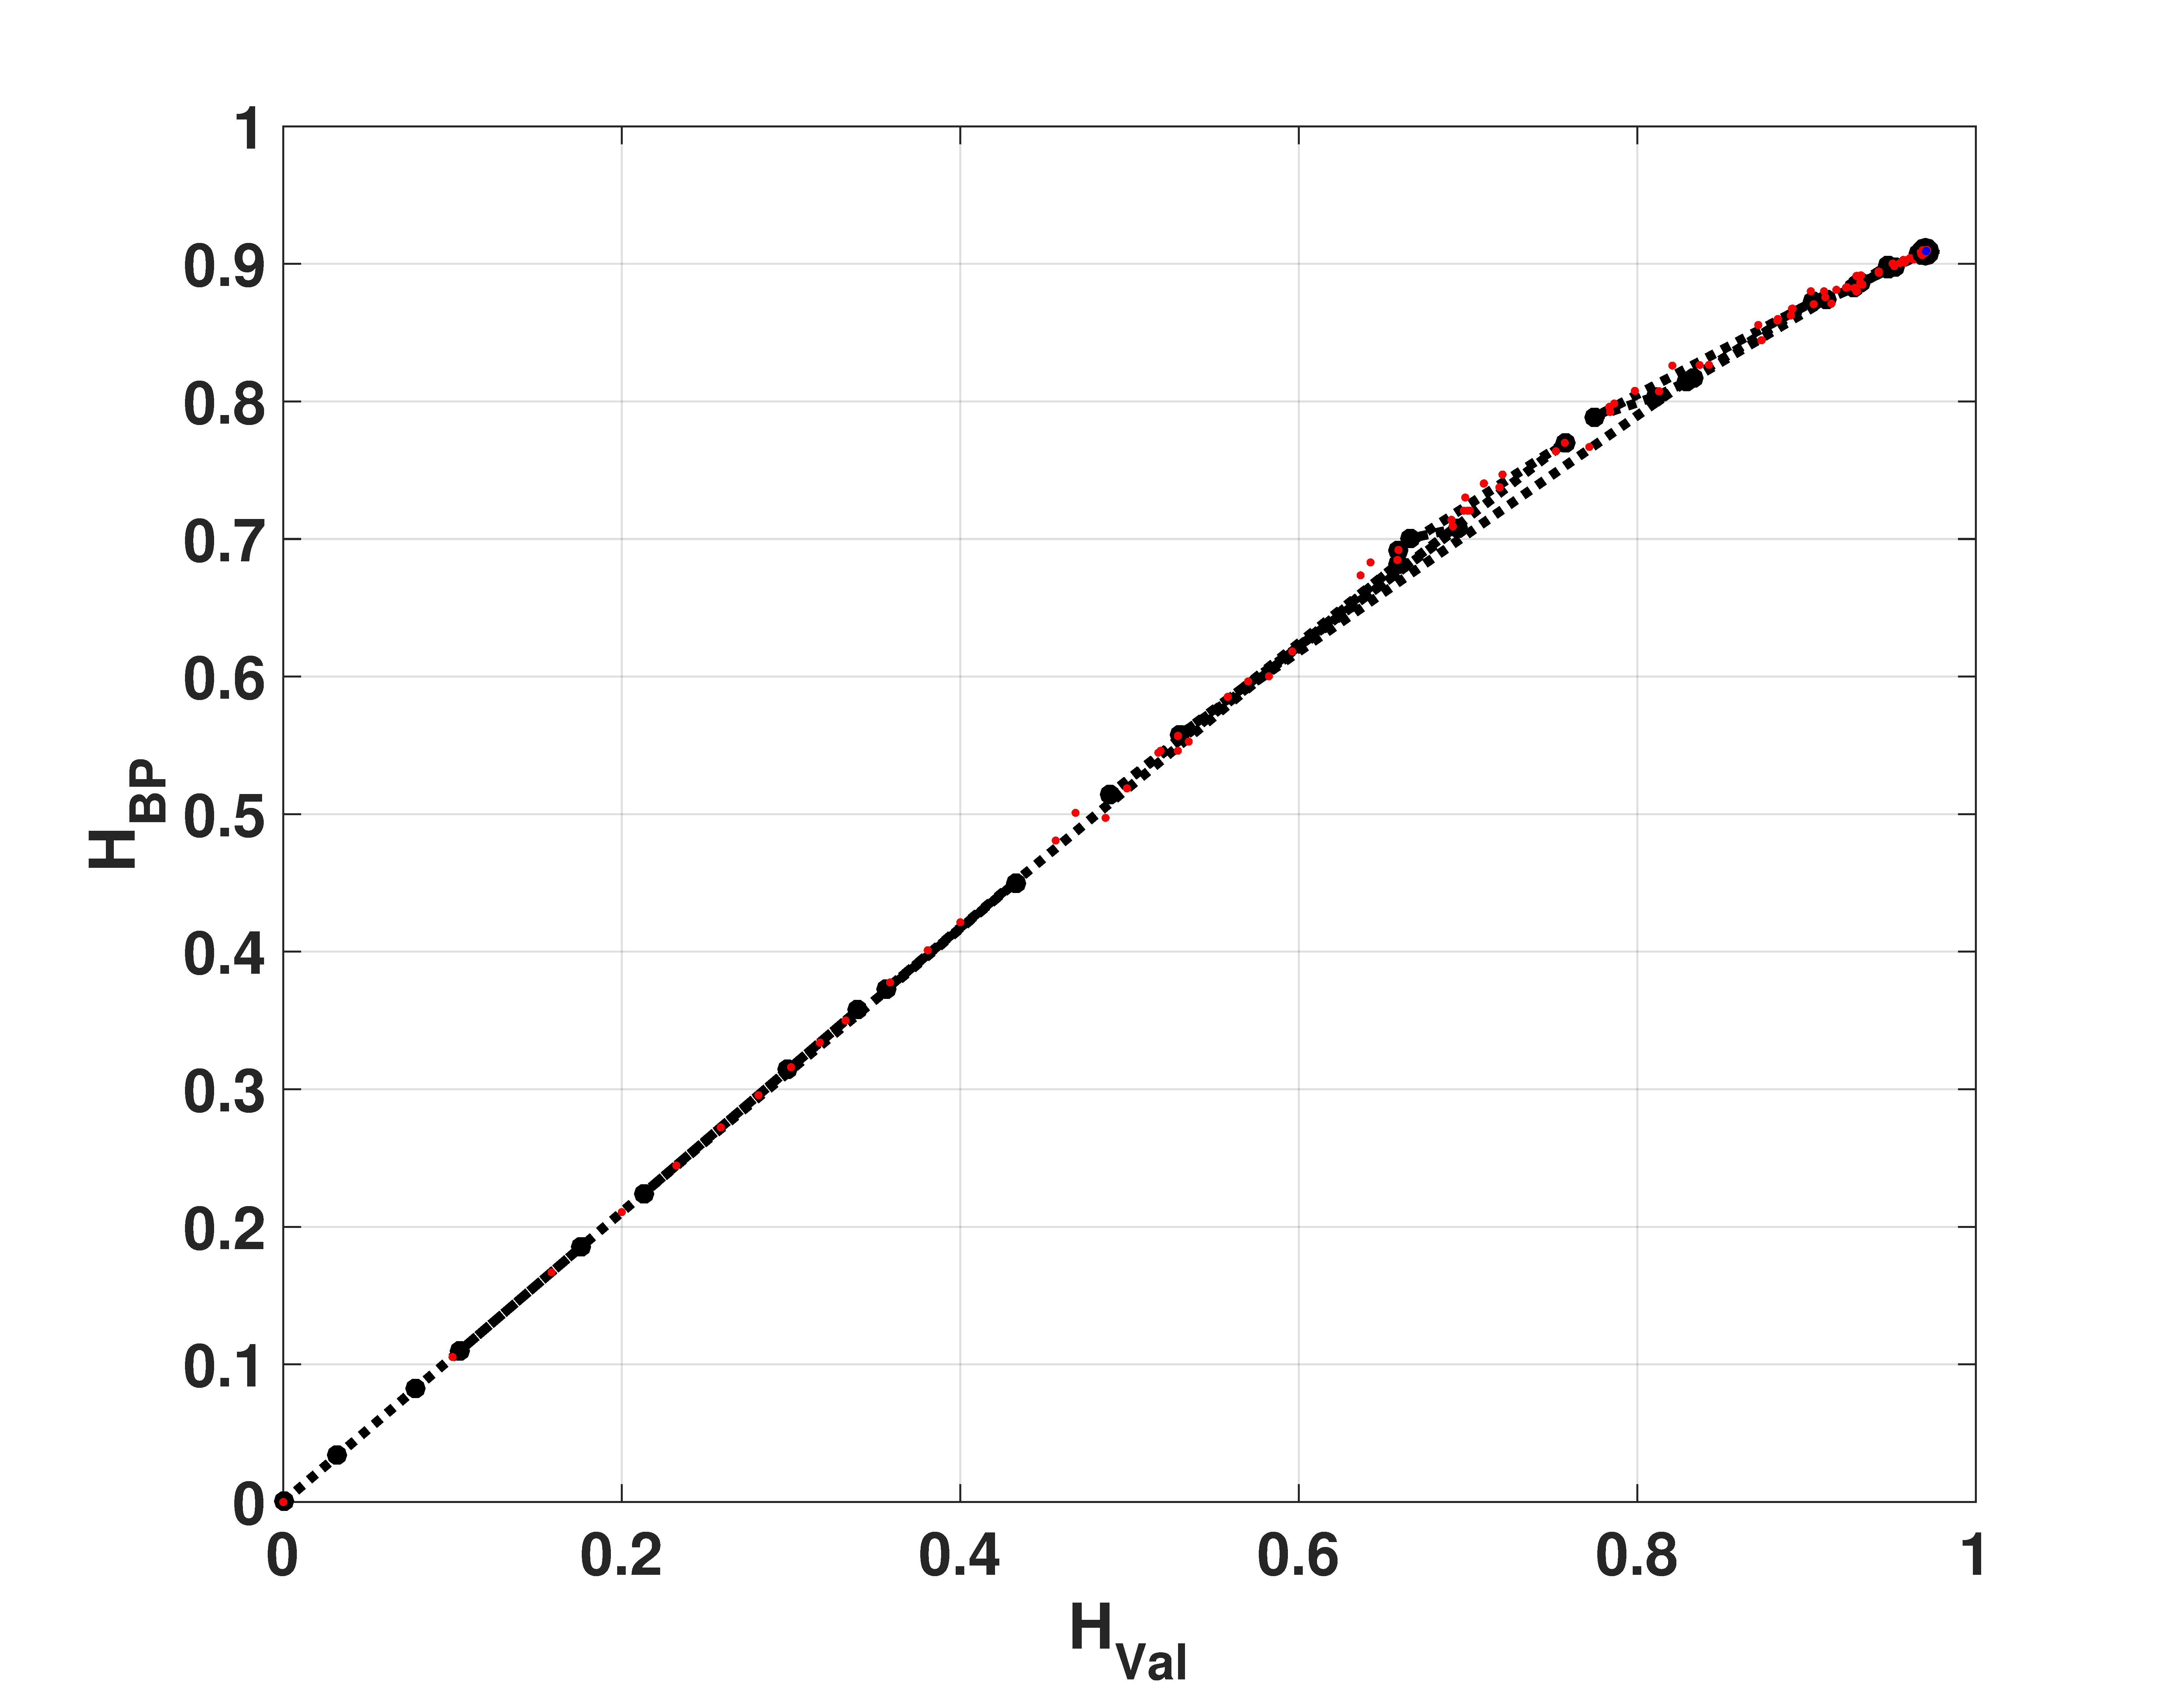
\includegraphics[width=.49\textwidth]{HbpHval_Odd}
	\caption{Evolution of statistical properties in double entropy plane for ODD map $H_{hist} \times H_{BP}$.}
	\label{fig:ODD_HH}
\end{figure}

Compatible results are shown in Figures \ref{fig:EVEN_HC} and \ref{fig:ODD_HC}, the position of asymptotic point is closest to the ideal point $(H_{hist}, H_{BP})=(1, 0)$.
This result reflects that mixing is better because the complexity of resulting system is lower.
This plane detects that the vector generated by ODD skipping is more mixed than EVEN.
%
\begin{figure}[H]
	\centering
	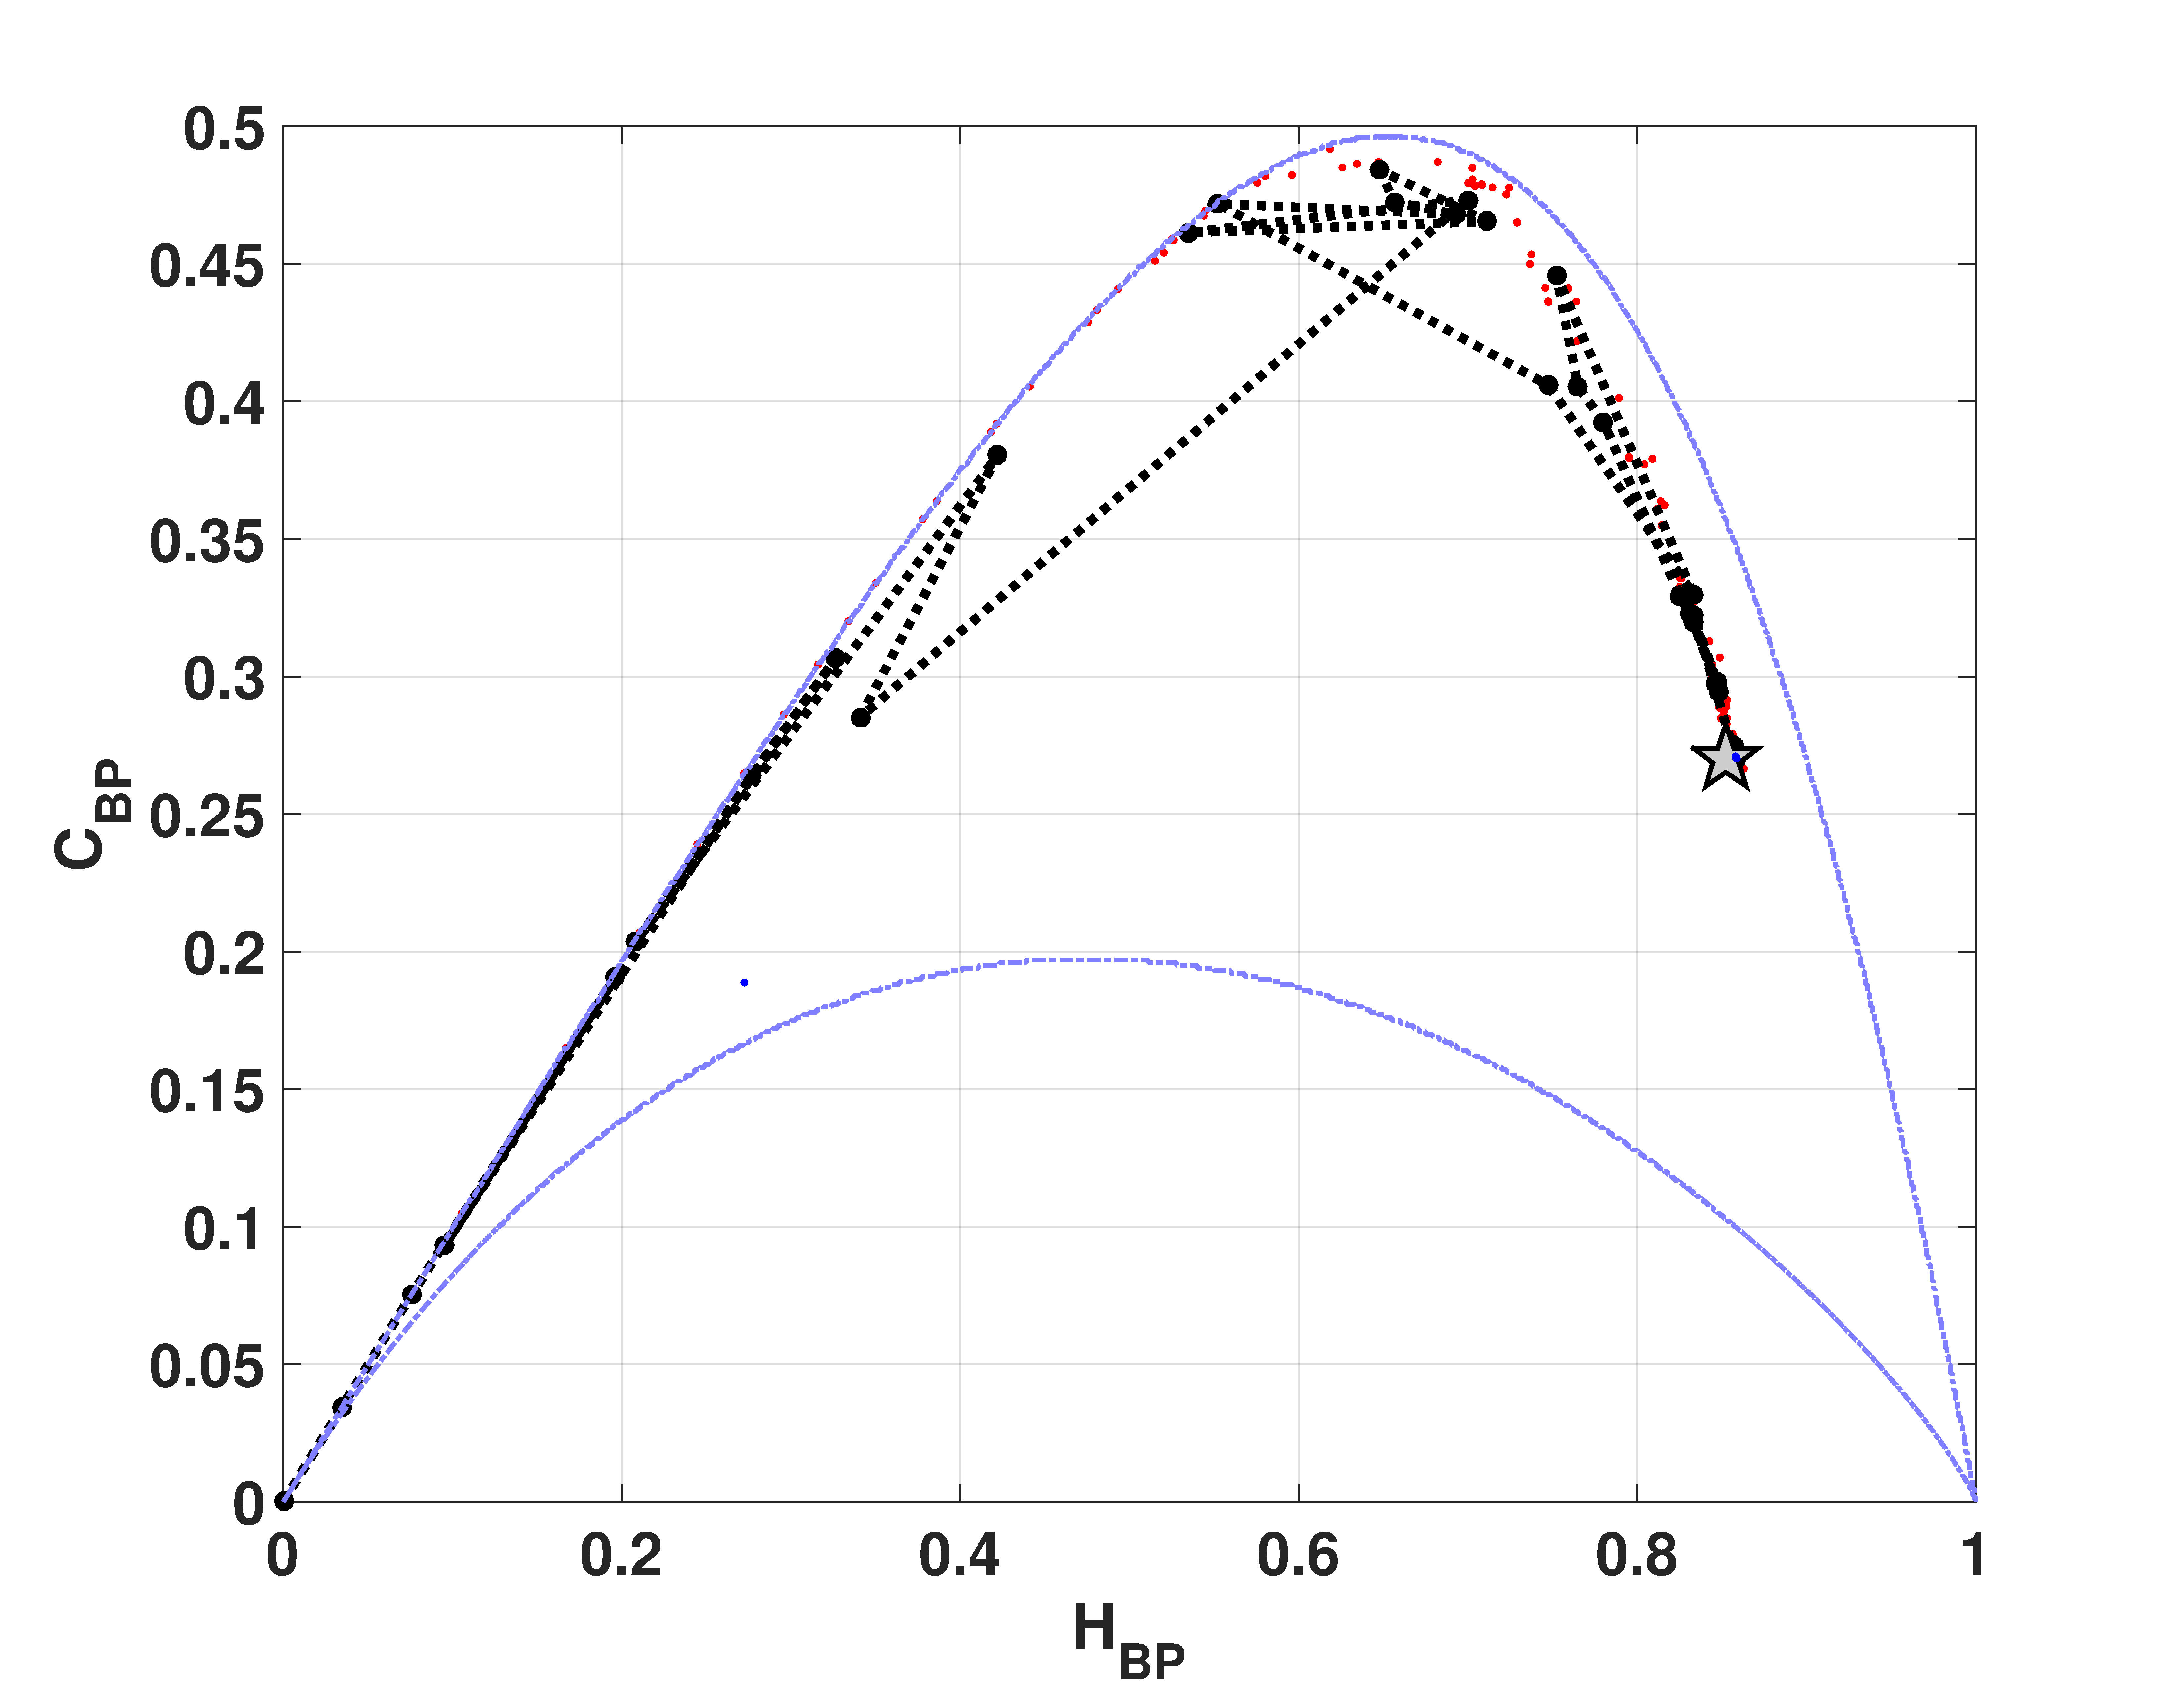
\includegraphics[width=.49\textwidth]{CbpHbp_Even}
	\caption{Evolution of statistical properties in entropy-complexity plane for EVEN map $H_{BP} \times C_{BP}$.}
	\label{fig:EVEN_HC}
\end{figure}
%
\begin{figure}[H]
	\centering
	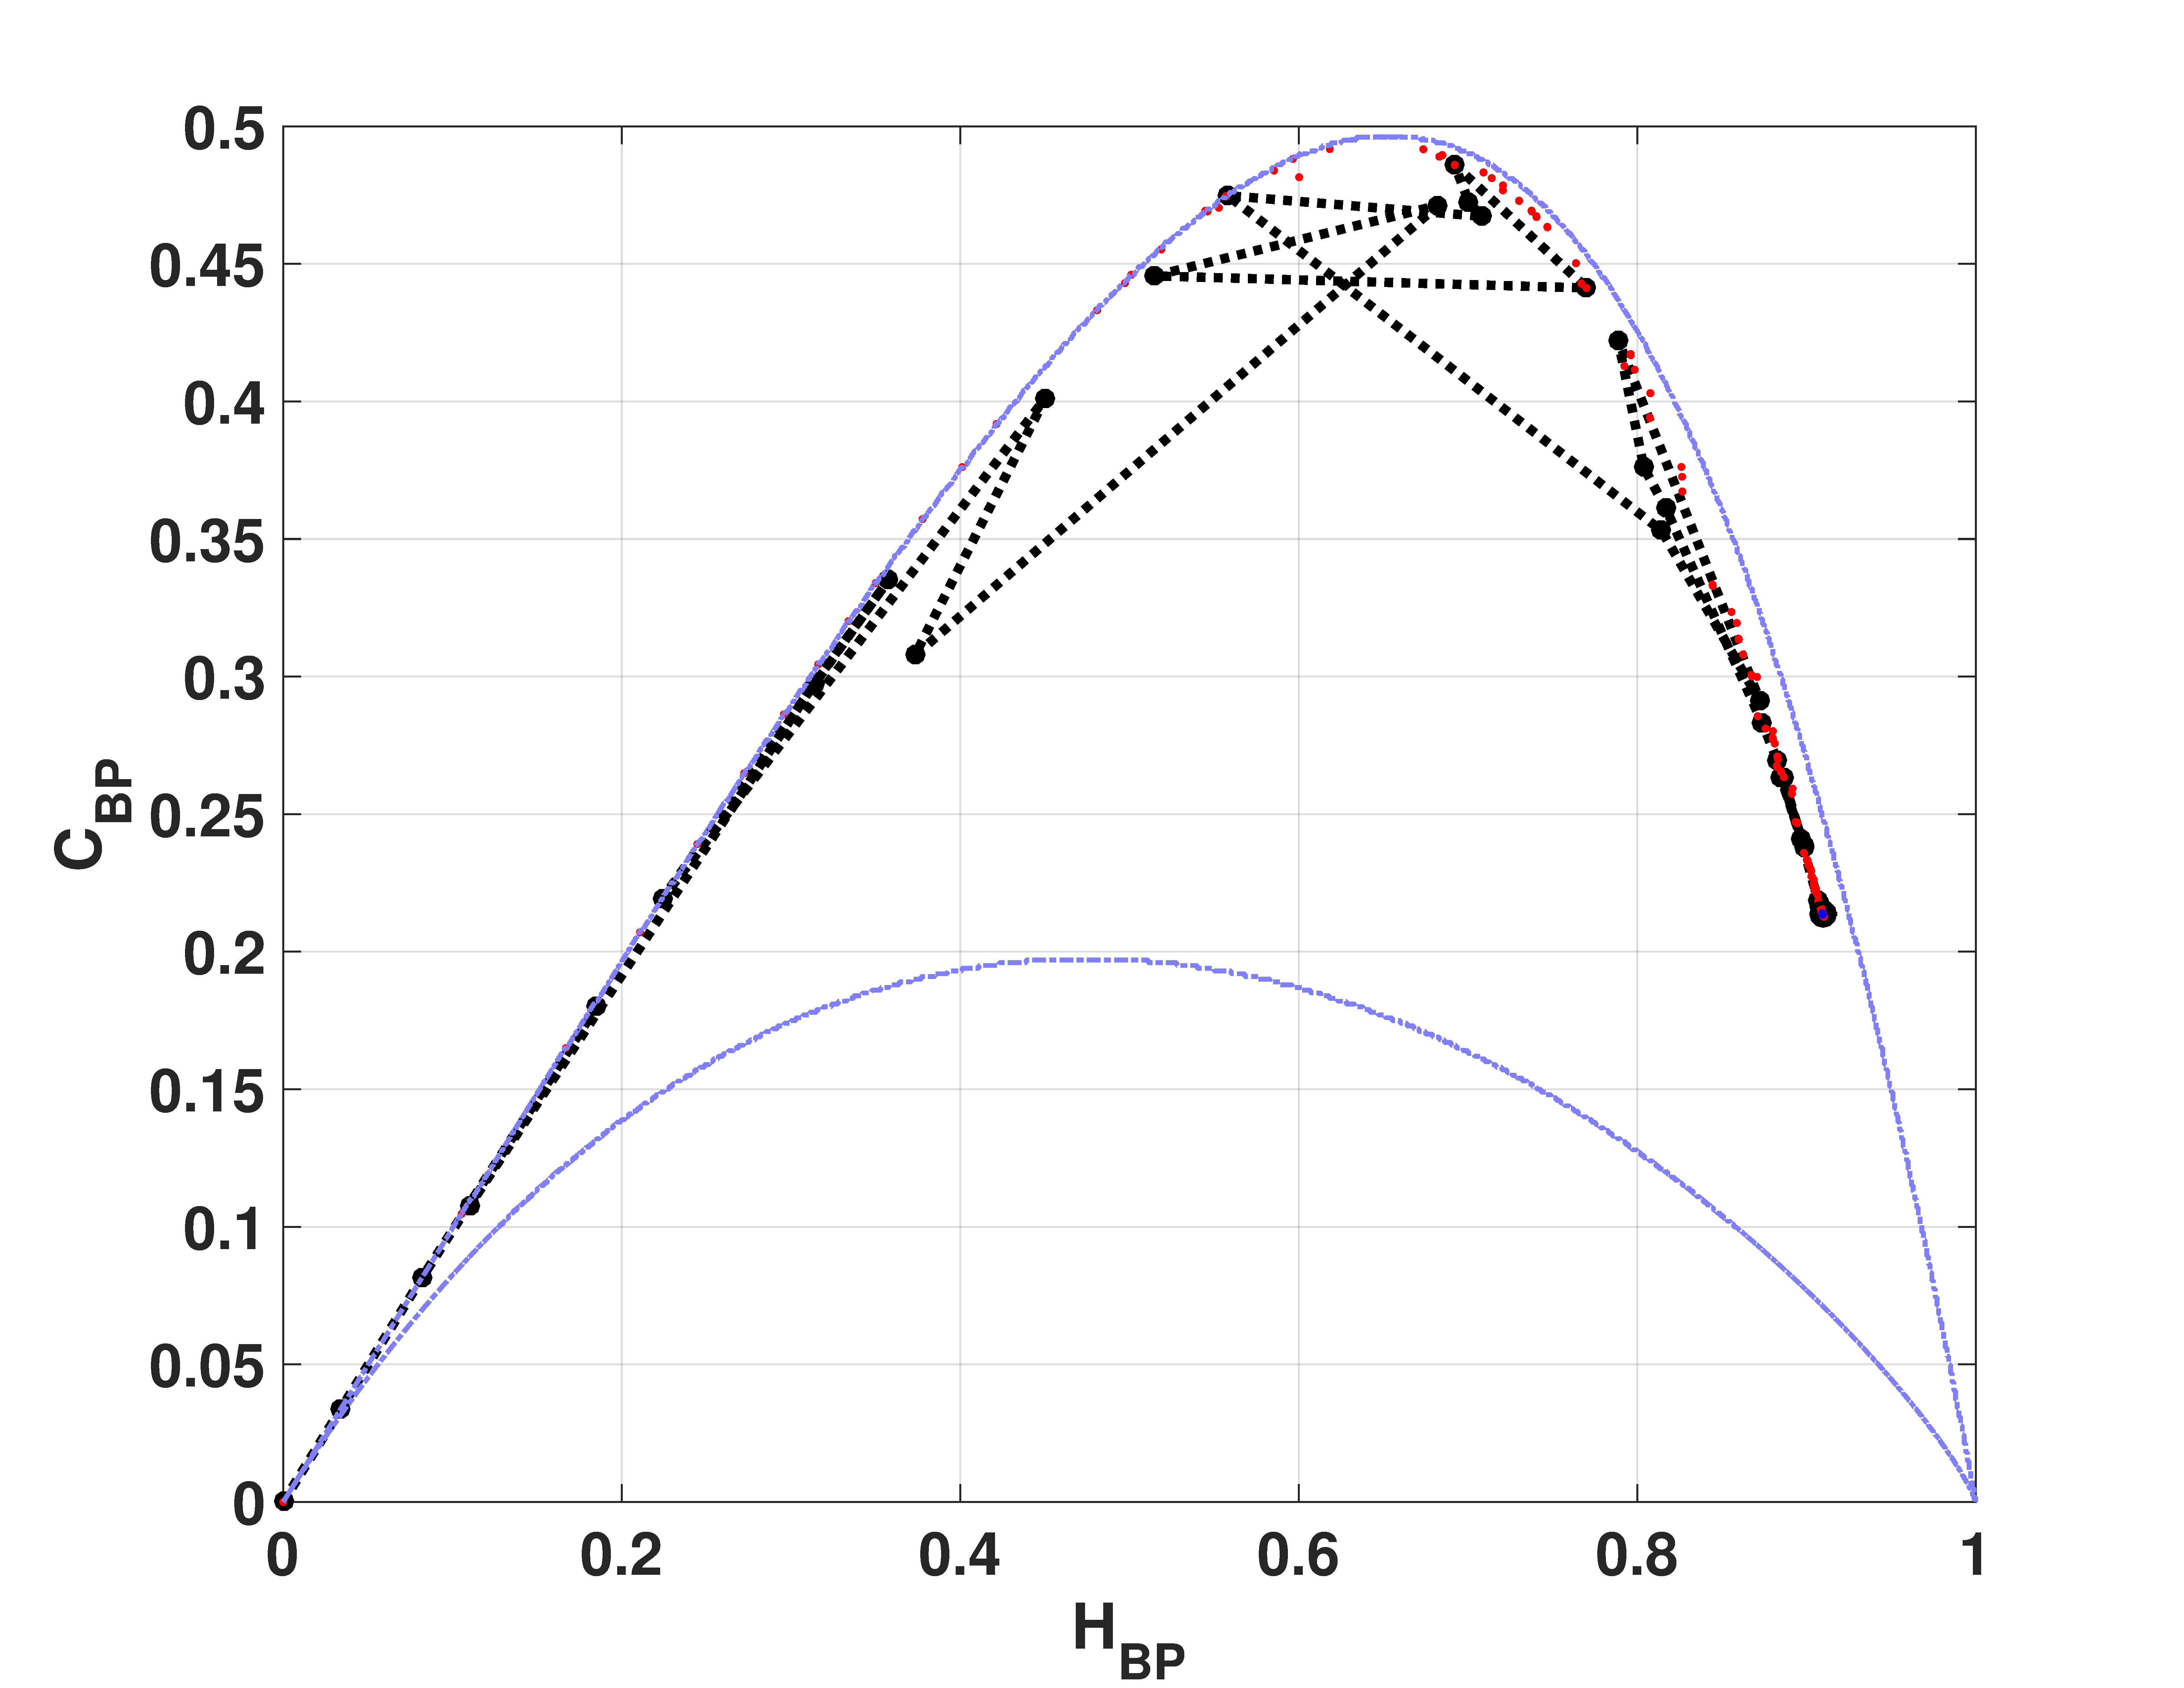
\includegraphics[width=.49\textwidth]{CbpHbp_Odd}
	\caption{Evolution of statistical properties in entropy-complexity plane for ODD map $H_{BP} \times C_{BP}$.}
	\label{fig:ODD_HC}
\end{figure}

\section{Conclusions}\label{sec:conclusions}
In summary:
\begin{itemize}
  \item Not every number base can be represented by a device with a certain base. For example, a base ten number can not be exactly represented in a conventional computer, it will always have an error inherent of the system..No todas las bases numéricas son representables con una máquina de base distinta. Por ejemplo, no se puede representar la base 10 con base 2.
  \item En una máquina de cálculo "a medida", como la que puede implementarse en ASICs o FPGAs existen limitaciones en el bus de datos y en la electrónica de cálculo. Si la electrónica de cálculo debe ser reducida se recomienda usar mapas que puedan ser calculados sólo con sumas y restas de la variable pseudoaleatoria.
  \item Los mapas que sólo tienen operaciones de shifteo en la base de la máquina de cálculo inevitablemente caerán a cero en tantas iteraciones como el largo de la mantisa de representación. Por ejemplo el tent en base 2.
  \item La comparación entre BP y BPW permite detectar el comportamiento del sistema. Puede detectarse si el atractor cae a un punto fijo y diferenciar si el transitorio es corto o largo, respecto de la cantidad de itaraciones del mapa.
  \item Como se menciona en el paper de referencia, el período del mapa iterado aumenta respecto del simple. También se nota una mejora marginal en la mezcla de la secuencia. La distribución de valores es buena en todos los casos.
  \item el skipping empeora el período pero mejora sustancialmente la mezcla de los valores. Esto puede verse en BP, BPW y MP.
\end{itemize}

produces a non-monotonous evolution toward the floating point result. This result is relevant because it shows that increasing the precision is not
always recommended.

ESTA FRASE ESTABA ARRIBA, VER DONDE LA PONEMOS: It is specially interesting to note that some systems (TENT) with very nice statistical properties in the world of the real numbers, become ``pathological" when binary numerical representations are used.


\bibliographystyle{elsarticle-num}
\bibliography{xbibwebdiciembre2013_ingles}

\end{document}
